% ============================================================================
% The Genesis Trilogy
% Complete Collected Volume
% ============================================================================

\documentclass[12pt,a4paper,openany]{book}

\usepackage[utf8]{inputenc}
\usepackage[T1]{fontenc}
\usepackage{amsmath,amssymb,amsfonts,amsthm}
\usepackage{mathtools}
\usepackage{mathrsfs}
\usepackage{physics}
\usepackage{graphicx}
\usepackage[hidelinks]{hyperref}
\usepackage{tikz}
\usetikzlibrary{shapes,arrows,positioning,calc,decorations.pathmorphing}
\usepackage{geometry}
\usepackage{fancyhdr}
\usepackage{titlesec}
\usepackage{array}
\newcolumntype{P}[1]{>{\raggedright\arraybackslash}p{#1}}
\usepackage{booktabs}
\usepackage{tcolorbox}
\usepackage{xcolor}
\usepackage{caption}
\usepackage{float}
\usepackage{enumitem}
\usepackage{newunicodechar}
\newunicodechar{आ}{\textit{aa}}
\newunicodechar{ल}{\textit{la}}
\newunicodechar{य}{\textit{ya}}
\newunicodechar{व}{\textit{va}}
\newunicodechar{ि}{\textit{i}}
\newunicodechar{ज}{\textit{ja}}
\newunicodechar{ञ}{\textit{~na}}
\newunicodechar{न}{\textit{na}}
\newunicodechar{श}{\textit{sha}}
\newunicodechar{ू}{\textit{uu}}
\newunicodechar{ण}{\textit{.na}}
\newunicodechar{त}{\textit{ta}}
\newunicodechar{ा}{\textit{aa}}
\newunicodechar{स}{\textit{sa}}
\newunicodechar{भ}{\textit{bha}}
\newunicodechar{ृ}{\textit{.r}}
\newunicodechar{ह}{\textit{ha}}
\newunicodechar{्}{}
\newunicodechar{§}{\S{}}
\newunicodechar{É}{\'{E}}
\newunicodechar{ñ}{\~{n}}
\newunicodechar{Ā}{\={A}}
\newunicodechar{ā}{\={a}}
\newunicodechar{ś}{\'{s}}
\newunicodechar{ū}{\={u}}
\newunicodechar{ṃ}{\d{m}}
\newunicodechar{ṅ}{\.{n}}
\newunicodechar{ṇ}{\d{n}}
\newunicodechar{—}{---}

\graphicspath{{Genesis_Trilogy_supplement/}{TDOME_I_supplement/}{TDOME_II_supplement/}{TDOME_III_supplement/}{TDOME_Complete_supplement/}}
\geometry{a4paper, margin=1in, headheight=28pt}

\newtheorem{theorem}{Theorem}[chapter]
\newtheorem{proposition}[theorem]{Proposition}
\newtheorem{lemma}[theorem]{Lemma}
\newtheorem{definition}[theorem]{Definition}
\newtheorem{remark}[theorem]{Remark}
\newtheorem{corollary}[theorem]{Corollary}
\newtheorem{conjecture}[theorem]{Conjecture}
\newtheorem{constraint}[theorem]{Constraint}
\newtheorem{example}[theorem]{Example}
\newtheorem{assumption}[theorem]{Assumption}
\newtheorem{criterion}[theorem]{Criterion}


\pagestyle{fancy}
\fancyhf{}
\fancyhead[LE,RO]{\thepage}
\fancyhead[RE]{\textit{The Genesis Trilogy}}
\fancyhead[LO]{\textit{\leftmark}}
\renewcommand{\headrulewidth}{0.4pt}

\title{
  \vspace{-2cm}
  {\Huge\textbf{The Genesis Trilogy}}\\[1cm]
  {\Large\textit{Emergent Geometry, Algebraic Persistence,\\ and the Architecture of the Observer}}\\[2cm]
  {\large Complete Collected Volume}\\[0.5cm]
  {\normalsize HAFF \textperiodcentered{} Q-RAIF \textperiodcentered{} T-DOME}
}

\author{
  \textbf{Sidong Liu, PhD}\\[0.5em]
  iBioStratix Ltd\\[0.3em]
  \texttt{sidongliu@hotmail.com}
}

\date{July 2026}

\begin{document}
\emergencystretch=2em
\raggedbottom
\hbadness=10000
\vbadness=10000

\frontmatter
\maketitle

\newpage
\thispagestyle{empty}
\vspace*{\fill}
\begin{center}
\textbf{Publication Record}\\[2em]
\begin{tabular}{ll}
Paper A & DOI: 10.5281/zenodo.18361706 \\
Paper B & DOI: 10.5281/zenodo.18367060 \\
Essay C & DOI: 10.5281/zenodo.18374805 \\
Paper D & DOI: 10.5281/zenodo.18388881 \\
Paper E & DOI: 10.5281/zenodo.18400065 \\
Paper F & DOI: 10.5281/zenodo.18400425 \\
Paper G & DOI: 10.5281/zenodo.18402907 \\
Postscript & DOI: 10.5281/zenodo.18407367 \\
Q-RAIF A & DOI: 10.5281/zenodo.18525876 \\
Q-RAIF B & DOI: 10.5281/zenodo.18525890 \\
Q-RAIF C & DOI: 10.5281/zenodo.18528934 \\
T-DOME I & DOI: 10.5281/zenodo.18574342 \\
T-DOME II & DOI: 10.5281/zenodo.18579703 \\
T-DOME III & DOI: 10.5281/zenodo.18591771 \\
\end{tabular}
\\[3em]
\textit{This collected volume compiles previously published works\\
for archival and reference purposes.}
\\[2em]
\copyright{} 2026 Sidong Liu. All rights reserved.
\end{center}
\vspace*{\fill}

\chapter*{Abstract}
\addcontentsline{toc}{chapter}{Abstract}

This volume collects the HAFF, Q-RAIF, and T-DOME papers comprising the Genesis Trilogy, a programme for studying how physical descriptions, persistent agents, and self-referential observers may be modelled within quantum theory.

The programme is organised in three parts.  HAFF studies observable-algebra accessibility and the conditional emergence of effective geometry, measurement, temporal records, and programme boundaries.  Q-RAIF studies Clifford-compatible algebraic encodings and image-level interfaces as modelling choices, not as a completed proof of uniqueness or algebraic necessity.  T-DOME studies memory, reference-frame selection, and self-referential calibration as a conditional architecture for specified persistent-agent models, not as a necessary, sufficient, minimal, or complete architecture for all agents.

Together, the three parts provide a calibrated structural research programme.  They supply conditional constructions, compatibility tests, and explicit open interfaces rather than a closed derivation of geometry, persistence, or consciousness from one theorem chain.

\bigskip
\noindent\textbf{Keywords}: emergent geometry, accessible algebras, coarse-graining, Clifford algebra, non-Markovian dynamics, reference-frame selection, Fisher information, self-referential calibration, Lyapunov stability, implementation cost

\tableofcontents

\mainmatter

% ============================================================================
% PART I: HAFF
% ============================================================================
\part{HAFF: The Holographic Alaya-Field Framework}
\label{part:HAFF}

% ============================================================================
% Paper A
% ============================================================================
\chapter{Emergent Geometry from Coarse-Grained Observable Algebras: The Holographic Alaya--Field Framework}
\label{H-chap:paperA}

\begin{center}
\textit{Paper A}\\[0.5em]
Originally published: Zenodo, DOI: 10.5281/zenodo.18361706
\end{center}

\bigskip

\section*{Abstract}
We construct a theoretical framework where the tensor factorization of a Hilbert space is treated as a structural variable rather than a kinematic background. 
By lifting the ``Alaya'' concept to a globally entangled vacuum state $|\Psi_{\text{vac}}\rangle$, we analyze how local geometric data may depend on specific observable subalgebras $\mathcal{A}_i \subset \mathcal{B}(\mathcal{H})$ when an explicit reconstruction dictionary is supplied. 
We show that, under a separating reconstruction dictionary, inequivalent entropy profiles induced by coarse-graining maps yield reconstructed geometric data not related by diffeomorphism.
The analysis is structural in nature: we do not propose new dynamics, but examine consistency and consequences of removing subsystem factorization from fundamental assumptions. 
This approach is complementary to existing interpretational frameworks and suggests natural connections to algebraic quantum field theory, entanglement-based approaches to spacetime, and quantum information theory.


\section{Introduction}

\subsection{Motivation}

Two central problems in contemporary theoretical physics concern the emergence of classicality and the emergence of geometry. 
In quantum foundations, the measurement problem asks how effectively classical behavior arises from an underlying quantum description. 
Decoherence theory has provided a powerful account of this process by explaining the suppression of interference between certain degrees of freedom through environmental entanglement \cite{Zurek2003}. 
However, this explanation typically presupposes a fixed decomposition of the total system into subsystems, distinguishing ``system,'' ``apparatus,'' and ``environment'' from the outset.

A closely related emergence problem appears in quantum gravity. 
A growing body of work suggests that spacetime geometry is not fundamental, but arises from patterns of quantum entanglement \cite{Maldacena1999,VanRaamsdonk2010}. 
In holographic settings, geometric quantities are related to entanglement measures via precise correspondences, most notably the Ryu--Takayanagi formula \cite{RyuTakayanagi2006}. 
Yet these constructions likewise assume a prior specification of spatial regions or tensor factors, with geometry inferred only after such a subdivision has been fixed.

In both contexts, the emergence problem is addressed only after a subsystem decomposition has been assumed.
The structure responsible for classicality or geometry is therefore explained relative to a partition whose origin remains largely unexamined.

\subsection{The Structural Gap}

The assumption of a given subsystem structure is often treated as innocuous, or as a matter of convenient description. 
However, from a fundamental perspective, there is no canonical tensor factorization of a generic Hilbert space, nor a unique way to decompose a global quantum state into subsystems.
While this issue is occasionally acknowledged in passing \cite{Zanardi2004,Viola2004}, its consequences for emergence are rarely explored systematically.

The present work does not challenge the empirical success of decoherence theory, entanglement-based approaches to geometry, or the algebraic formulation of quantum theory.
Rather, we make explicit a structural assumption common to these frameworks and investigate the consequences of relaxing it.
Our focus is on what follows if subsystem structure itself is treated as emergent, rather than fundamental.

\subsection{Our Contribution}

We formulate a framework in which subsystem structure is not assumed \emph{a priori}, but arises from a choice of coarse-graining over observable algebras.
Within this framework, we show that different coarse-graining channels can induce inequivalent effective states and connectivity data.  In a holographic or other reconstruction model that separates the resulting entropy profiles modulo diffeomorphisms, this difference can induce inequivalent effective geometries.  Outside such a dictionary, the output is a weighted connectivity structure, not a spacetime metric.

The analysis is structural in nature.
Our aim is not to propose a new dynamical mechanism, but to examine the consistency and consequences of removing subsystem factorization from the set of fundamental assumptions.

\subsection{Terminology: The Alaya-Field}

Throughout this work, we adopt the term \emph{Alaya-Field} to denote the fundamental, non-factorized structure prior to any subsystem decomposition.
This terminology, borrowed from Yogācāra philosophy (referring to the ``storehouse consciousness''), is used here strictly in a technical sense.

In what follows, the Alaya-Field does not refer merely to a vector in Hilbert space, but to the triple
\[
(\mathcal{H}_U, \mathcal{A}_U, |\Omega\rangle),
\]
where $\mathcal{A}_U$ is a von Neumann algebra acting on $\mathcal{H}_U$ and $|\Omega\rangle$ is a cyclic and separating vector.
The emphasis is on the absence of a canonical factorization, not on the particular choice of state.

In an AQFT realization, $\mathcal A_U$ may be a Type~III$_1$ factor and $|\Omega\rangle$ a cyclic and separating vector \cite{Haag1996}.  This is a possible source-side regime, not a consequence of the finite-dimensional calculations below, and we do not infer localized eigenmodes or a metric from the Type~III label alone.
This usage is intended to evoke the non-factorized, pre-geometric nature of the fundamental quantum structure, without importing any metaphysical commitments.

\subsection{Regime of Each Result}

The paper uses a mixed regime.  The source triple $(\mathcal H_U,\mathcal A_U,|\Omega\rangle)$ may be discussed for a general von Neumann algebra, including Type~III under the stated cyclic-and-separating hypothesis.  The factorization, Haar measure, density-matrix, partial-trace, and von Neumann-entropy results in Sections~\ref{H-A-sec:nopref}--\ref{H-A-sec:geometry} are finite-dimensional/Type~I results.  Type~III factors have no density matrices or trace entropy, so those results are not asserted there.  The conversion from entropy/connectivity data to a spacetime metric is a separate model-dependent holographic input.

\subsection{Structure of the Paper}

The paper is organized as follows.
In Section~\ref{H-A-sec:nopref}, we review the absence of a canonical subsystem decomposition in quantum theory and formalize this observation.
Section~\ref{H-A-sec:coarse} introduces coarse-graining in terms of observable algebras and analyzes how effective subsystem descriptions arise from this procedure.
In Section~\ref{H-A-sec:geometry}, we construct coarse-graining-dependent connectivity data, give a state-space QFIM construction, and state the additional reconstruction hypothesis required before metric inequivalence can be claimed.
Section~\ref{H-A-sec:discussion} discusses the scope and conceptual implications of the framework, its relation to existing approaches, and possible directions for future work.
We conclude in Section~\ref{H-A-sec:conclusion} with a summary of results and open questions.

\section{Absence of Canonical Tensor Factorization}
\label{H-A-sec:nopref}

\subsection{The Factorization Problem}

In standard quantum mechanics, the state space of a composite system is constructed as a tensor product of subsystem Hilbert spaces. 
This construction presupposes that a natural decomposition into subsystems has already been identified. 
However, for a given Hilbert space $\mathcal{H}_{\text{total}}$, there is no unique or canonical way to express it as a tensor product $\mathcal{H}_A \otimes \mathcal{H}_B$ without additional physical input.

The universal entanglement statement used in an earlier version is withdrawn.  Indeed, fix dimensions $d_A,d_B>1$ with $d_Ad_B=\dim\mathcal H_{\mathrm{total}}$.  For any pure state $|\Psi_U\rangle$, choose a unitary $U$ sending a reference product vector $|0\rangle_A\otimes|0\rangle_B$ to $|\Psi_U\rangle$.  Pulling the reference tensor factors through $U$ gives a nontrivial factorization in which $|\Psi_U\rangle$ is a product.  Thus no finite-dimensional pure state is entangled across \emph{every} nontrivial factorization.

What does survive is a fixed-family typicality result.

\begin{theorem}[Entanglement typicality for a specified family]
\label{H-A-thm:nofact}
Let $\mathcal H_{\mathrm{total}}$ be finite dimensional and let
$\mathfrak F=\{\mathbf f_1,\ldots,\mathbf f_m\}$ be a finite family of
nontrivial tensor factorizations selected by a physical rule independent
of the sampled state.  Write
$\mathcal H_{\mathrm{total}}=\mathcal H_{A_j}\otimes\mathcal H_{B_j}$
with $d_{A_j}\le d_{B_j}$.  For $\delta>0$, let
\[
p_j(\delta):=
\Pr_{\Psi\sim\mathrm{Haar}}
\left[S(\rho_{A_j})<\log d_{A_j}-\delta\right].
\]
Then
\[
\Pr\left[
S(\rho_{A_j})\ge\log d_{A_j}-\delta
\text{ for every }j
\right]
\ge 1-\sum_{j=1}^m p_j(\delta),
\]
and the standard concentration estimates make each $p_j(\delta)$ small
at large dimension under the usual dimension-ratio hypotheses.
\end{theorem}

\begin{proof}
For each fixed $\mathbf f_j$, Page's theorem gives~\cite{Page1993}
\begin{equation}
\label{H-A-eq:page}
\mathbb{E}[S(\rho_{A_j})]
=\sum_{k=d_{B_j}+1}^{d_{A_j}d_{B_j}}\frac1k
-\frac{d_{A_j}-1}{2d_{B_j}},
\end{equation}
while concentration of measure bounds the lower tail~\cite{HaydenLeungWinter2006}; this is precisely $p_j(\delta)$.  Applying the union bound to the finite, preselected family proves the displayed inequality.
\end{proof}

\begin{remark}[What the theorem does not select]
Theorem~\ref{H-A-thm:nofact} says nothing about all possible factorizations and supplies no preferred member of $\mathfrak F$.  Specifying the admissible family and its selection rule is a quantum-mereology input, not a consequence of Haar typicality.  Developing that input is an open problem; see \cite{Cotler2019,CarrollSingh2021}.
\end{remark}

\begin{remark}[Relation to prior work]
The observation that tensor product structures are not canonical was recognized early in the foundations of quantum theory, and has been systematically analyzed in work on virtual subsystems and quantum mereology \cite{Zanardi2001,Zanardi2004,Cotler2019,CarrollSingh2021}.
Their work demonstrated that subsystem decompositions are effectively determined by sets of accessible observables rather than being intrinsic to the Hilbert space.
The present framework extends this perspective to the context of holographic geometry and entanglement-based spacetime emergence, where the choice of observable algebra determines not only subsystem structure but also the emergent geometric description.
\end{remark}

\begin{remark}
We do not claim that subsystem decompositions are impossible or unphysical, but that they are not uniquely determined by the universal quantum state alone. 
This observation motivates the search for additional structure that specifies how a subsystem decomposition arises in concrete physical contexts.
\end{remark}

\subsection{Relation to Algebraic Approaches}

The absence of a canonical factorization has been recognized in various contexts, including algebraic quantum field theory where observable algebras take precedence over tensor product structures \cite{Haag1996}.
Our framework builds on these insights by treating coarse-graining structure as the fundamental input from which subsystem decompositions emerge.

\section{Observer-Dependent Coarse-Graining and Effective States}
\label{H-A-sec:coarse}

\subsection{Coarse-Graining Structure}

Before introducing the formal definition, we emphasize that the introduction of an observable algebra does not reinstate a tensor factorization. 
Operators may act irreducibly on $\mathcal{H}_{\text{total}}$ without inducing any subsystem decomposition. 
In algebraic quantum field theory, observable algebras are defined independently of any global tensor product structure \cite{Haag1996}.
Furthermore, a coarse-graining is not selected by an agent, but instantiated by a concrete physical interaction structure.

\begin{definition}[Operational Coarse-Graining Structure]
\label{H-A-def:coarse}
Let $\mathcal{H}_U$ be the universal Hilbert space. 
A \textbf{coarse-graining structure} $\mathbf{c}$ is defined as a pair
\[
\boxed{\mathbf{c} \equiv (\mathcal{A}_{\mathrm{sel},\mathbf{c}}, \Phi_{\mathbf{c}})}
\]
where:
\begin{enumerate}
\item $\mathcal{A}_{\mathrm{sel},\mathbf{c}} \subset \mathcal{B}(\mathcal{H}_U)$ is a selected unital $*$-subalgebra used to define the effective representation.  It is not identified with Paper~E's probe-reachable effect system, pointer/record algebra, or environmental fixed set; a physical model must state any map between them.
\item In the finite-dimensional results below, $\Phi_{\mathbf{c}}$ is a CPTP map on states implementing an operational reduction, and its Heisenberg dual $\Phi_{\mathbf c}^*$ is unital and completely positive.  Examples include partial trace over a specified factor and channels induced by a conditional expectation.  In a general von Neumann setting the corresponding object would be a normal channel on states with a normal UCP dual, but no entropy theorem below is asserted merely from that extension.
\end{enumerate}
\end{definition}

\begin{remark}[Non-uniqueness of observable algebras]
It is important to note that the specification of a selected algebra $\mathcal{A}_{\mathrm{sel},\mathbf{c}}$ is not assumed to be unique.
In algebraic quantum field theory and quantum information theory, there exists no theorem guaranteeing a unique maximal observable algebra associated with a given physical system without additional structure. 
The coexistence of multiple admissible algebras reflects physical underdetermination rather than subjectivity or observer dependence.
\end{remark}

\subsection{Refinement Structure of Coarse-Grainings}

\begin{definition}[Refinement Relation]
\label{H-A-def:refine}
Given two coarse-graining structures $\mathbf{c}_1, \mathbf{c}_2$, we say $\mathbf{c}_1 \succeq \mathbf{c}_2$ if there exists a CPTP map
\[
\Lambda: \mathcal{B}(\mathcal{H}_{\text{eff}}(\mathbf{c}_1)) \to \mathcal{B}(\mathcal{H}_{\text{eff}}(\mathbf{c}_2))
\]
such that
\[
\Phi_{\mathbf{c}_2} = \Lambda \circ \Phi_{\mathbf{c}_1}
\]
In this case, $\mathbf{c}_2$ is a \textbf{further coarse-graining} of $\mathbf{c}_1$.
\end{definition}

\begin{remark}[Multiplicity of coarse-graining maps]
For a fixed selected algebra $\mathcal{A}_{\mathrm{sel},\mathbf{c}}$, there generally exist multiple completely positive trace-preserving maps implementing distinct coarse-graining procedures.
The present framework does not require the selection of a preferred CPTP map. 
Rather, different maps correspond to physically realizable information-loss mechanisms, such as tracing over inaccessible degrees of freedom or effective decoherence channels.
\end{remark}

Different coarse-graining choices are related not by unitary symmetry, but by information-theoretic refinement maps, forming a partially ordered structure rather than a group.

\subsection{Core Theorem}

The absence of a unitary intertwiner and the distinction of observable images were previously presented as conclusions, although they merely unpacked (and in the case of the images did not follow from) the chosen inequivalence relation.  They are not retained as theorem claims.  The nontrivial finite-dimensional statement is the following generic separation result.

\begin{theorem}[Generic separation for a fixed pair of channels]
\label{H-A-thm:inequiv}
Let $\mathcal H$ and $\mathcal K=\mathcal K_A\otimes\mathcal K_{A^c}$ be finite dimensional, and let $\Phi_1\ne\Phi_2$ be two CPTP maps from states on $\mathcal H$ to states on the common output space $\mathcal K$.  Then the pure inputs on which $\Phi_1$ and $\Phi_2$ agree form a Haar-null proper real-algebraic subset.  If, in addition, the real-analytic function
\[
f_A(\Psi):=
S\!\left(\operatorname{Tr}_{A^c}\Phi_1(|\Psi\rangle\!\langle\Psi|)\right)
-S\!\left(\operatorname{Tr}_{A^c}\Phi_2(|\Psi\rangle\!\langle\Psi|)\right)
\]
is not identically zero on each connected component under consideration of the open set where both reduced outputs are full rank, then $f_A(\Psi)\ne0$ for generic inputs in those components.
\end{theorem}

\begin{proof}
Because pure-state projectors span the Hermitian operators, $\Phi_1-\Phi_2$ cannot vanish on every pure projector.  The equality condition is polynomial in the real and imaginary components of $|\Psi\rangle$, so its solution set is a proper real-algebraic subset and has Haar measure zero.  On the full-rank domain, von Neumann entropy and hence $f_A$ are real analytic.  A nonzero real-analytic function has a measure-zero zero set, proving the conditional entropy statement.
\end{proof}

\begin{remark}
The nondegeneracy hypothesis on $f_A$ is essential: distinct channels related by a unitary acting only on $A$ can produce different states with identical subsystem entropy for every input.  The theorem therefore does not turn channel inequivalence alone into entanglement or geometric inequivalence.
\end{remark}

\begin{remark}[Relation to decoherence theory]
We emphasize that the present framework is fully compatible with standard decoherence theory and does not modify its dynamical content. 
Decoherence successfully explains the emergence of classical behavior given a fixed system--environment decomposition. 
The novelty of the present approach lies instead in treating such subsystem decompositions as coarse-graining--dependent and not fundamental.
\end{remark}

\subsection{Clarification on Subsystem Structure}

Subsystems are not fundamental inputs to the framework, but derived representations induced by a chosen observable algebra. 
The connectivity measure defined in Section~\ref{H-A-sec:geometry} acts on these representations, and is not used to define the algebra itself. 
The causal order is:
\[
\text{Observable Algebra} \to \text{Representation} \to \text{Entanglement} \to \text{Connectivity} \to \text{Geometry}
\]
No geometric structure is presupposed in the definition of coarse-graining.

\subsection{Algebraic Perspective on Subsystems}

A potential concern is whether the use of observable algebras implicitly presupposes a subsystem decomposition. 
We stress that this is not the case. 
Observable algebras need not be defined via a tensor factorization of the total Hilbert space.

In algebraic quantum field theory, local algebras are assigned to spacetime regions without invoking a global tensor product structure \cite{Haag1996}. 
Subsystems arise only at the level of representations induced by a chosen algebra, rather than serving as its foundational input. 
In this sense, subsystem structure is emergent rather than fundamental.

\begin{remark}[Subsystems as induced representations]
Within the present framework, subsystems are not primitive entities. 
They emerge as representations associated with a given observable algebra and coarse-graining structure. 
This avoids circularity by reversing the usual explanatory order: observable structure precedes subsystem identification.
\end{remark}

\section{Entanglement Structure and Emergent Geometry}
\label{H-A-sec:geometry}

\subsection{Mutual Information as Connectivity Measure}

We stress that no geometric structure is assumed in the definition of the coarse-graining introduced in Section~\ref{H-A-sec:coarse}. 
Geometry only appears at the level of entanglement relations between the induced subsystems.

Given a coarse-graining structure $\mathbf{c} = (\mathcal{A}_{\mathrm{sel},\mathbf c},\Phi_{\mathbf c})$ as defined in Section~\ref{H-A-sec:coarse}, the universal quantum state $|\Psi_U\rangle$ induces a family of effective subsystems $\{A,B,\dots\}$ associated with subalgebras of $\mathcal{A}_{\mathrm{sel},\mathbf c}$.
For any such pair of subsystems $A$ and $B$, we consider the quantum mutual information
\begin{equation}
I_{\mathbf{c}}(A:B) = S_{\mathbf{c}}(A) + S_{\mathbf{c}}(B) - S_{\mathbf{c}}(AB),
\end{equation}
where $S_{\mathbf{c}}(\cdot)$ denotes the von Neumann entropy computed after coarse-graining.

\begin{definition}[Entanglement-Induced Connectivity]
\label{H-A-def:connectivity}
Let $A$ and $B$ be two disjoint subsystems induced by $\mathbf{c}$.
We define an effective \textbf{proximity measure} $\mu_{\mathbf{c}}(A,B)$ based on the quantum mutual information:
\begin{equation}
\mu_{\mathbf{c}}(A,B) := I_{\mathbf{c}}(A:B) = S(\rho_A) + S(\rho_B) - S(\rho_{AB}).
\end{equation}
While $\mu_{\mathbf{c}}$ does not itself constitute a metric (as it violates the triangle inequality), it defines a weighted connectivity graph in a declared subsystem representation.
\end{definition}

Here is the precise finite-dimensional information-geometric construction used when a metric on a \emph{parameter space of coarse-grained states} is needed.  Let $\lambda\mapsto\rho_{\mathbf c}(\lambda)$ be a smooth faithful family and define the symmetric logarithmic derivatives $L_a$ by
\[
\partial_a\rho_{\mathbf c}
=\frac12\bigl(L_a\rho_{\mathbf c}+\rho_{\mathbf c}L_a\bigr).
\]
The SLD quantum Fisher metric is
\begin{equation}
g^{\mathrm{QF}}_{ab}(\lambda)
:=\frac12\operatorname{Tr}\!\left[
\rho_{\mathbf c}(\lambda)\{L_a,L_b\}\right].
\label{H-A-eq:qfim}
\end{equation}
This is a positive-semidefinite Riemannian metric on identifiable parameter directions.  It is not a Lorentzian spacetime metric, and it is not determined by the pairwise numbers $\mu_{\mathbf c}(A,B)$ without an additional map from graph/state parameters to geometry.  In the holographic discussion below that additional map is a reconstruction dictionary, not a general consequence of QFIM \cite{Petz1996}.

This quantity should be understood as a \emph{connectivity measure} rather than a fundamental spacetime distance.
In general, mutual information does not define a metric on arbitrary quantum subsystems.
However, it acquires a natural geometric interpretation under physically motivated assumptions, which we make explicit below.

\paragraph{Assumptions.}
Throughout this section, we restrict attention to coarse-grainings that satisfy a geometric admissibility condition:

\begin{definition}[Geometric Admissibility]
\label{H-A-def:geoadmit}
A coarse-graining structure $\mathbf{c}$ is said to be \textbf{geometrically admissible} if the induced mutual information satisfies:
\begin{enumerate}
\item \emph{Finite correlation length:} The state $|\Psi_U\rangle$ exhibits exponentially decaying correlations with respect to the induced subsystems, as is typical for gapped systems, ground states of local Hamiltonians, and holographic large-$N$ states.
\item \emph{Monotonic decay under refinement:} Mutual information decreases monotonically as subsystems become more refined.
\item \emph{Stability under perturbations:} The entanglement structure is robust under small perturbations of $\Phi_{\mathbf{c}}$.
\end{enumerate}
\end{definition}

Not all coarse-grainings admit a geometric interpretation. 
Geometry is not generic; it is a \emph{special phase} of information organization.
We further assume coarse-graining consistency: all entropic quantities are computed using a single coarse-graining structure $\mathbf{c}$, avoiding any mixing of inequivalent observable algebras.

Under these assumptions, the entanglement-induced connectivity $\mu_{\mathbf{c}}(A,B)$ is non-negative, symmetric, and vanishes if and only if the subsystems are uncorrelated at the level resolved by $\mathbf{c}$.
Moreover, in regimes where mutual information decays monotonically with separation, $\mu_{\mathbf{c}}$ induces an effective notion of spatial proximity.

\begin{remark}
The connectivity $\mu_{\mathbf{c}}(A,B)$ should be understood as an \emph{effective, coarse-graining--dependent measure of correlation}, rather than a fundamental spacetime metric.
A metric on a state-family parameter space may be supplied by Eq.~\eqref{H-A-eq:qfim}.  A spacetime metric requires the additional reconstruction input stated below.
\end{remark}

In a continuum limit of densely overlapping subsystems, the collection $\{\mu_{\mathbf{c}}(A,B)\}$ may approximate a weighted graph with a geometric interpretation.  This is a model-building step: neither graph convergence nor a map from the QFIM parameter metric to spacetime is established in general.

\subsection{From Entanglement to Geometry}

The idea that spacetime geometry is encoded in quantum entanglement has been explored extensively in the context of holography.
In particular, the Ryu--Takayanagi formula relates the entanglement entropy of a boundary region $A$ to the area of an extremal surface $\gamma_A$ in the bulk \cite{RyuTakayanagi2006},
\begin{equation}
S(A) = \frac{\mathrm{Area}(\gamma_A)}{4G_N},
\end{equation}
suggesting a direct correspondence between entanglement structure and geometric data.

More generally, Van Raamsdonk has argued that the connectivity of spacetime is controlled by the pattern of entanglement between subsystems \cite{VanRaamsdonk2010}.
In this perspective, highly entangled degrees of freedom correspond to nearby regions in the emergent geometry, while weakly entangled subsystems are geometrically distant.

The entanglement-induced connectivity $\mu_{\mathbf{c}}(A,B)$ provides a concrete realization of this idea.
Given a collection of subsystems induced by $\mathbf{c}$, the mutual information defines a weighted graph whose vertices correspond to subsystems and whose edge weights encode entanglement strength.

In tensor network constructions such as MERA, similar entanglement graphs admit a natural geometric interpretation, with graph distance approximating continuum spatial distance \cite{Swingle2012}.
In particular tensor-network or holographic models, an appropriate continuum limit can be equipped with an effective Riemannian spatial geometry whose metric reflects the underlying entanglement structure.

In this sense, geometry emerges not as an additional postulate, but as an effective description of how information is distributed and shared among coarse-grained degrees of freedom.

\subsection{Coarse-Graining Dependence of Geometry}

We now turn to the central observation of this section: the emergent geometry depends essentially on the choice of coarse-graining structure.

\begin{theorem}[Coarse-graining dependent geometry, conditional reconstruction]
\label{H-A-thm:geom}
Let $\mathbf{c}_1$ and $\mathbf{c}_2$ act on the same finite-dimensional global state and induce entropy profiles $S_1,S_2$.  Assume a specified reconstruction dictionary $\mathfrak G$ is defined on both profiles and is separating modulo diffeomorphisms on the compared class:
\[
\mathfrak G[S_1]\simeq_{\mathrm{diff}}\mathfrak G[S_2]
\quad\Longrightarrow\quad
S_1\simeq_{\mathfrak G}S_2.
\]
If $S_1\not\simeq_{\mathfrak G}S_2$, then the reconstructed metrics $\mathfrak G[S_1]$ and $\mathfrak G[S_2]$ are not related by a diffeomorphism.  The theorem makes no metric claim when no such dictionary is supplied.
\end{theorem}

\begin{proof}
This is the contrapositive of the separating property of $\mathfrak G$.  Holographic entropy/area reconstruction is one setting in which such a property may be established on a restricted state class \cite{RyuTakayanagi2006}.  Channel inequivalence by itself does not provide either the hypothesis $S_1\not\simeq_{\mathfrak G}S_2$ or the dictionary.
\end{proof}

\begin{example}[Free Fermion Chain: Spatial vs.\ Momentum Coarse-Graining]
\label{H-A-ex:fermion}
Consider $N$ free fermions on a one-dimensional lattice with ground state $|\Psi_0\rangle$.

\textbf{Spatial coarse-graining} $\mathbf{c}_x$: group sites into blocks of $k$ consecutive sites.
By the area law for gapped free-fermion chains~\cite{Eisert2010}, the entanglement entropy of a block of $L$ sites satisfies $S(L) \sim \mathrm{const}$, independent of $L$.
The mutual information between blocks $A$ and $B$ separated by distance $r$ decays exponentially as $I(A:B) \sim e^{-r/\xi}$, where $\xi$ is the correlation length set by the spectral gap~\cite{Hastings2007}.
The resulting connectivity graph has short-range edges: its graph distance approximates a one-dimensional lattice, yielding a line-like emergent geometry.

\textbf{Momentum-mode coarse-graining} $\mathbf{c}_p$: use the occupation-number tensor factors of the diagonal momentum modes.  A free-fermion ground state is a Slater determinant
\[
|\Psi_0\rangle=\prod_{k\in F}c_k^\dagger|0\rangle,
\]
which is a product of filled or empty occupation states in this factorization.  Every subset of momentum modes therefore has a pure reduced state and disjoint momentum subsets have zero mutual information.  The momentum connectivity graph is empty, not a volume-law, long-range graph.  Wolf's result \cite{Wolf2006} concerns \emph{spatial} entanglement scaling in fermionic systems and does not support momentum-mode entanglement.

Thus the example demonstrates dependence of connectivity on a specified factorization: the spatial representation can carry short-range edges, while the free momentum-occupation representation carries none.  It does not exhibit two reconstructed geometries; indeed $\mathbf c_p$ fails the geometric-admissibility goal unless further, interacting correlations or a separate reconstruction prescription are supplied.
\end{example}

A simple conceptual illustration is provided by contrasting spatial coarse-graining with momentum-space coarse-graining.
In the former case, entanglement typically obeys an area law and supports a local, connected geometry.
For the free Slater determinant, the latter has no momentum-mode entanglement at all; interacting models would be required to obtain a nontrivial momentum graph.
Importantly, both descriptions arise from the same underlying state $|\Psi_U\rangle$.

Thus, the geometry inferred from entanglement is not an intrinsic property of the quantum state alone, but depends on how information is rendered accessible through coarse-graining.

\subsection{Beyond Coordinate Choice}

It is important to distinguish the dependence described above from an ordinary change of coordinates.
A diffeomorphism acts within a fixed algebra of observables, preserving the underlying notion of what is measurable.
By contrast, a change of coarse-graining alters the observable algebra itself, modifying which correlations are accessible and how subsystems are defined.

These are categorically distinct operations.  Nevertheless, algebraic inequivalence alone does not prove that two reconstructed metrics fail to be diffeomorphic: a reconstruction dictionary may discard the algebraic differences.  Non-diffeomorphism follows only under the separating hypothesis of Theorem~\ref{H-A-thm:geom}.  Without it, the justified conclusion is that the effective operator or connectivity descriptions differ.

We return to the conceptual implications of this distinction in the Discussion.

\begin{figure}[ht]
\centering
\begin{tikzpicture}[>=stealth, auto, node distance=3cm]
    % Styles
    \tikzstyle{state} = [circle, draw, thick, fill=gray!10, minimum size=2.5cm, align=center]
    \tikzstyle{filter} = [rectangle, draw, thick, fill=white, minimum width=2.5cm, minimum height=1cm]
    \tikzstyle{geo} = [ellipse, draw, thick, dashed, minimum width=2.5cm, minimum height=1.5cm, align=center]
    
    % Nodes
    \node[state] (Alaya) {Global State\\$|\Psi_{\text{vac}}\rangle$\\(Alaya-Field)};
    
    \node[filter] (Filter1) [below left of=Alaya, xshift=-1cm, yshift=-1cm] {Algebra $\mathcal{A}_1$};
    \node[filter] (Filter2) [below right of=Alaya, xshift=1cm, yshift=-1cm] {Algebra $\mathcal{A}_2$};
    
    \node[geo] (Geo1) [below of=Filter1, yshift=-1cm] {Geometry $M_1$\\($g_{\mu\nu}^{(1)}$)};
    \node[geo] (Geo2) [below of=Filter2, yshift=-1cm] {Geometry $M_2$\\($g_{\mu\nu}^{(2)}$)};
    
    % Arrows
    \draw[->, thick] (Alaya) -- node[left, font=\footnotesize] {Coarse Grain $\Phi_1$} (Filter1);
    \draw[->, thick] (Alaya) -- node[right, font=\footnotesize] {Coarse Grain $\Phi_2$} (Filter2);
    
    \draw[->, double, thick] (Filter1) -- node[left, font=\footnotesize] {Induces} (Geo1);
    \draw[->, double, thick] (Filter2) -- node[right, font=\footnotesize] {Induces} (Geo2);
    
    % Interaction
    \draw[<->, dotted, very thick] (Geo1) -- node[below, font=\footnotesize] {Inequivalent ($M_1 \not\cong M_2$)} (Geo2);

\end{tikzpicture}
\caption{Schematic of the conditional HAFF construction. A single global state is reduced by two coarse-graining channels. The outputs define different effective connectivity data; only a stated reconstruction dictionary promotes them to metrics $g_{\mu\nu}^{(1,2)}$. The dependence is on coarse-graining at the level of effective description, not on an observer in a fundamental sense.}
\label{H-A-fig:haff_scheme}
\end{figure}

\section{Discussion}
\label{H-A-sec:discussion}

\subsection{Relation to Existing Frameworks}

The framework developed in this work is not intended as a replacement for existing interpretational or algebraic approaches to quantum theory.
Rather, it is best understood as orthogonal to several well-established lines of thought, addressing a distinct structural question.
In this section, we briefly clarify its relation to three representative frameworks:

\subsubsection{Relation to QBism}

QBism emphasizes the role of agents and their personal probability assignments in quantum theory, interpreting the quantum state as an expression of subjective belief rather than an objective property of a system.
In contrast, the present framework assumes a single, objective global quantum state throughout.
No agent-dependent elements enter the formalism, and no interpretational commitments regarding belief, experience, or decision theory are required.

The point of contact lies solely in the rejection of a privileged subsystem decomposition.
While QBism attributes this absence to the primacy of the agent, our framework treats it as a structural feature of quantum theory itself.
Coarse-grainings are not chosen by agents, but instantiated by concrete physical interaction structures.
The resulting multiplicity of effective descriptions reflects physical underdetermination rather than subjectivity.

\subsubsection{Relation to Many-Worlds and Decoherence-Based Approaches}

Many-Worlds--type interpretations and decoherence-based accounts provide a compelling explanation of classical behavior within quantum mechanics by analyzing branching structures relative to a fixed subsystem decomposition.
Our framework does not modify this analysis, nor does it introduce an alternative account of branching or classicality.

The difference lies at a prior level.
Decoherence theory presupposes a tensor factorization into system, apparatus, and environment.
Here, we instead ask how such subsystem structures arise in the first place.
In this sense, the framework is complementary to decoherence-based approaches: it leaves their dynamical conclusions intact while removing subsystem factorization from the list of fundamental assumptions.

\subsubsection{Relation to Algebraic Quantum Field Theory}

The closest structural affinity of the present work is with algebraic quantum field theory (AQFT).
In AQFT, observable algebras are taken as primary, and states are defined as positive linear functionals over these algebras, without reliance on a global tensor product structure.
Our use of observable algebras and their representations is directly inspired by this tradition.

The present framework may be viewed as extending this algebraic perspective by emphasizing the role of coarse-graining relations between algebras.
Different choices of coarse-graining induce different effective representations and, consequently, different entanglement structures.
The novelty lies not in the algebraic formalism itself, but in using it to analyze the emergence and non-uniqueness of geometric descriptions.

Taken together, these comparisons situate the present work as a structural investigation into the conditions under which subsystem structure and geometry emerge.
It neither commits to a particular interpretation of quantum mechanics nor proposes a new dynamical law, but instead clarifies how several existing frameworks implicitly rely on assumptions that can be made explicit and, in some cases, relaxed.

\subsection{Scope and Limitations}

The present work is concerned with structural consistency rather than phenomenological prediction. 
Observable consequences depend on the physical mechanisms implementing a given coarse-graining, which lie beyond the scope of this paper. 
This is analogous to effective field theory, where multiple UV completions may share the same low-energy structure. 
Future work will explore concrete physical realizations and their empirical signatures.

\subsection{Philosophical Implications}

We emphasize that the framework assumes a single, objective global quantum state $|\Psi_U\rangle$. 
What is coarse-graining--dependent is not reality itself, but the effective structures used to describe it. 
This position is compatible with scientific realism while acknowledging the role of operational context in physical description.

\subsection{Future Directions}

While the present work is deliberately limited to a structural analysis of subsystem emergence and geometry within a fixed global quantum state, it naturally opens several directions for further investigation. 
We emphasize that the following points are not results established here, but rather indicate possible extensions where the current framework may provide useful conceptual or technical guidance.

\subsubsection{Dynamical Models of Coarse-Graining Selection}

In this work, coarse-graining structures are treated as fixed relational inputs, instantiated by concrete physical interaction patterns. 
A natural next step is to investigate whether such coarse-grainings can themselves be characterized dynamically.

One possible direction is to study how interaction Hamiltonians, coupling strengths, or network topologies bias the emergence of particular subalgebra structures over others, in contact with explicit quantum-mereology and locality-selection programmes \cite{Cotler2019,CarrollSingh2021}.
This could clarify under what physical conditions certain factorizations become robust or persistent, and whether transitions between inequivalent coarse-grainings admit an effective dynamical description.

Importantly, such an analysis would remain compatible with globally unitary evolution, treating coarse-graining selection as an emergent, effective phenomenon rather than a modification of fundamental dynamics.

\subsubsection{Connections to Quantum Information and Complexity}

The non-uniqueness of emergent geometry highlighted here suggests a close connection to quantum information--theoretic notions such as entanglement structure, operator complexity, and resource constraints.

Future work could explore whether preferred geometric descriptions correlate with informational criteria---for example, minimal description length, stability under noise, or computational accessibility of observables. 
Such considerations may help explain why certain coarse-grainings are physically salient, even when many are formally admissible.

This perspective may also provide a bridge to recent work on complexity-based approaches to spacetime emergence, without committing to any particular complexity measure at the present stage.

\subsubsection{Extensions to Quantum Field Theory and Continuum Limits}

While the framework has been formulated in abstract Hilbert space terms, an important open question concerns its implementation in quantum field--theoretic settings, where issues of locality, algebraic nets, and continuum limits arise.

In particular, it would be valuable to examine how coarse-graining relations between observable algebras interact with the locality structures emphasized in algebraic quantum field theory, and whether familiar spacetime geometries can be recovered as stable fixed points of such relations.

We stress that the present work does not resolve these questions, but provides a structural language in which they can be posed more precisely.

\subsubsection{Empirical and Phenomenological Implications}

At the level developed here, the framework is primarily structural and conceptual. 
Nevertheless, future investigations may ask whether different coarse-graining choices lead to distinguishable effective descriptions, for example in semiclassical regimes, quantum gravity--motivated models, or analogue systems.

Such studies could clarify whether the non-uniqueness of emergent geometry has observable consequences, or whether physical constraints effectively suppress this freedom in realistic settings.

Any empirical analysis would necessarily require additional assumptions beyond those adopted in this work, and thus lies outside its present scope.

\subsubsection{Conceptual Clarifications and Interpretational Interfaces}

Finally, although the framework is intentionally neutral with respect to interpretations of quantum mechanics, it may serve as a useful interface for comparative studies. 
By making explicit the structural assumptions underlying subsystem decomposition and geometry, it could help clarify which features are interpretation-dependent and which arise more generally from the formalism itself.

We view this not as an attempt to adjudicate between interpretations, but as an opportunity to sharpen the questions they address.

\medskip

Taken together, these directions suggest that the framework developed here is best viewed as a scaffold: it does not dictate specific physical models, but provides a structured setting in which questions about subsystems, geometry, and emergence can be formulated with greater precision.

\section{Conclusion}
\label{H-A-sec:conclusion}

We have presented a framework in which subsystem structure is not presupposed, but is modelled through coarse-graining over selected observable algebras. 
The central results are:

\begin{enumerate}
\item For a finite, physically preselected family of factorizations, Haar-typical states are highly entangled across every member under the stated dimension hypotheses (Theorem~\ref{H-A-thm:nofact}); no claim is made over all possible factorizations or about a preferred factorization.
\item For a fixed pair of distinct finite-dimensional channels, their outputs are generically separated; a generic entropy difference requires the explicit non-degeneracy hypothesis in Theorem~\ref{H-A-thm:inequiv}.
\item When a separating reconstruction dictionary is supplied and the compared entropy profiles are inequivalent in its declared sense, the reconstructed geometric data are not related by a diffeomorphism (Theorem~\ref{H-A-thm:geom}).
\end{enumerate}

The framework is deliberately limited in scope. 
We have not proposed new dynamics, derived empirical predictions, or resolved interpretational debates. 
Instead, we have examined the structural consequences of removing subsystem factorization from the list of fundamental assumptions.

Within the stated channel and reconstruction hypotheses, this investigation shows how geometric data can depend on the chosen coarse-graining context. 
It does not establish a geometry for an arbitrary quantum state or coarse-graining without an additional reconstruction dictionary. 
This perspective is compatible with, and complementary to, existing approaches including decoherence theory, holographic duality, and algebraic quantum field theory.

Several open questions remain. 
Can coarse-graining structures themselves be characterized dynamically? 
Do informational or complexity-based criteria select physically preferred coarse-grainings? 
Can the framework be extended to quantum field theory and reconciled with standard locality structures? 
These questions lie beyond the present scope, but the structural setting developed here provides a language in which they can be formulated with greater precision.

Ultimately, this work suggests that the relationship between quantum states, subsystems, and geometry is more subtle than the standard picture implies. 
By making explicit an assumption that is often left implicit, we hope to have clarified the conditions under which emergence occurs and opened new avenues for investigating the foundations of quantum theory and spacetime.

\section*{Acknowledgments}

The author thanks the anonymous reviewers for their insightful comments and suggestions, which greatly improved the clarity and rigor of this work.

% ============================================================================
% Paper B
% ============================================================================
\chapter{Accessibility, Stability, and Emergent Geometry: Conceptual Clarifications on the Holographic Alaya--Field Framework}
\label{H-chap:paperB}

\begin{center}
\textit{Paper B}\\[0.5em]
Originally published: Zenodo, DOI: 10.5281/zenodo.18367060
\end{center}

\bigskip

\section*{Abstract}
This paper provides conceptual clarification of the Holographic Alaya-Field Framework (HAFF) introduced in our previous work. 
We address three potential misreadings: subjectivism (that observers create spacetime), anti-realism (that geometry is illusory), and trivialism (that the framework reduces to coordinate choice). 
By analyzing the structural notion of accessibility via stability conditions, delineating boundaries with existing interpretations (AQFT, RQM, QBism, MWI), and characterizing emergent geometry as a stable organizational phase, we clarify what the framework commits to and what it does not. 
This analysis is purely interpretational; no new formal results are introduced.


\section{Introduction}
\label{H-B-sec:intro}

Our previous work proposed a framework in which effective operator and connectivity descriptions depend on a selected algebra acting on a global quantum state \cite{Liu2026}.  Metric inequivalence is conditional on a reconstruction dictionary; it is not a general consequence of channel or algebra inequivalence.
However, structural novelty of this kind is particularly vulnerable to interpretational confusion. 
The present paper addresses these interpretational implications and clarifies the conceptual commitments of the framework.

\subsection{The Risk of Misreading}

The claim that geometry is coarse-graining-dependent naturally invites several misreadings, each of which conflates distinct notions of dependence. 
Three such misreadings are especially common:

\begin{enumerate}
\item \emph{Subjectivism}: The view that observers or agents create spacetime through their choices or beliefs, collapsing the framework into an epistemic or observer-relative interpretation.
\item \emph{Anti-realism}: The view that spacetime has no objective existence, and that emergent geometry is therefore illusory or merely pragmatic.
\item \emph{Trivialism}: The view that coarse-graining-dependent geometry reduces to a choice of coordinates or descriptive convention, with no substantive physical consequences.
\end{enumerate}

Each of these readings is incorrect, but each arises naturally from surface-level features of the formalism. 
The purpose of this paper is to block such misreadings by clarifying the nature of accessibility, the structural role of observable algebras, and the ontological status of emergent geometry within the framework.

\subsection{Scope and Objectives}

This paper introduces no theorems.  The stability criteria and phase quantities below are explicitly heuristic diagnostics and model inputs, not proved selection principles.  The paper provides a systematic interpretational analysis aimed at three specific objectives:

\begin{enumerate}
\item \emph{Clarify the notion of accessibility}: We formulate accessibility as a structural and operational modelling proposal relative to declared dynamics, probes, and mereology, rather than as an epistemic or observer-dependent notion.
\item \emph{Delineate boundaries with existing interpretations}: We situate the framework in relation to algebraic quantum field theory, relational quantum mechanics, QBism, and the Many-Worlds interpretation, clarifying points of agreement, divergence, and complementarity.
\item \emph{Characterize the ontological status of emergent geometry}: We argue that geometry functions as a stable organizational phase of quantum information, analogous to phases in condensed matter systems, avoiding both naive realism and anti-realist eliminativism.
\end{enumerate}

Importantly, this analysis does not constitute a defense of the framework, nor does it aim to persuade readers of its correctness. 
The goal is clarity: to ensure that the structural commitments of the framework are understood on their own terms, and that criticisms, if any, are directed at what the framework actually claims rather than at interpretational projections.

\subsection{What This Paper Does Not Do}

To further delimit scope, we note explicitly what this paper does \emph{not} attempt:

\begin{itemize}
\item It does not propose new dynamics, empirical predictions, or modifications to quantum mechanics.
\item It does not claim that the framework resolves outstanding problems in quantum gravity, quantum foundations, or the measurement problem.
\item It does not advocate for any particular metaphysical or philosophical position beyond the minimal structural commitments required by the formalism itself.
\item It does not interpret the framework as implying idealism, observer-created reality, or any form of mind-dependence.
\end{itemize}

The analysis remains strictly within the domain of structural interpretation: identifying what the mathematical formalism commits to, what it leaves open, and how it relates to existing approaches.

\subsection{Organization}

The paper proceeds as follows. Section~\ref{H-B-sec:stance} briefly recapitulates the structural stance adopted in our previous work, emphasizing the priority of observable algebras over tensor factorizations and the role of coarse-graining in defining effective subsystems. 

Section~\ref{H-B-sec:accessibility} provides a detailed analysis of candidate accessibility diagnostics and their physical inputs. A taxonomy distinguishes subjective, relational, and structural notions of dependence; HAFF adopts the third as a model-relative proposal without claiming a unique input-free selector.

Section~\ref{H-B-sec:relations} examines the relationship between the framework and four representative approaches: algebraic quantum field theory, relational quantum mechanics, QBism, and the Many-Worlds interpretation. Each subsection clarifies points of conceptual overlap and structural divergence, preventing conflation while identifying opportunities for complementarity.

Section~\ref{H-B-sec:geometry_phase} argues that emergent geometry should be understood as a stable organizational phase of entanglement structure, drawing on analogies with condensed matter physics. This perspective avoids treating geometry as either fundamental or illusory, instead characterizing it as contingent but objective—dependent on physical conditions rather than epistemic contexts.

Section~\ref{H-B-sec:scope} delimits the structural assumptions of the framework, enumerates what it does not commit to, and outlines open questions for future investigation. Particular attention is given to the distinction between structural analysis and metaphysical advocacy.

\subsection{Methodological Note}

Throughout this paper, we adopt a deliberately conservative rhetorical stance. Claims are hedged with modal qualifiers ("may suggest," "is consistent with," "can be understood as") because the selection criteria and phase analogy are heuristic and because interpretational conclusions should not outrun their model inputs. The goal is to present the framework as one coherent way of organizing the conceptual landscape, not as the uniquely correct interpretation.

This methodological caution reflects a broader commitment: interpretational clarity is best served by precision and restraint, not by advocacy or polemics. We aim to make the framework legible to researchers across different interpretational traditions, facilitating comparison and critique rather than preempting it.

\section{Structural Stance Recap}
\label{H-B-sec:stance}

We briefly recapitulate the structural stance of our previous work without repeating full mathematical derivations.

The framework uses three claims with different epistemic status:
\begin{enumerate}
\item \textbf{Factorization input}: Hilbert-space structure alone supplies no preferred tensor factorization.  Paper~A proves entanglement typicality only for a finite, physically preselected family; choosing that family remains a quantum-mereology input.

\item \textbf{Conditional channel separation}: Distinct finite-dimensional coarse-graining channels generically produce different outputs.  Entropy separation requires an explicit nondegeneracy condition.

\item \textbf{Conditional geometry}: Entropy/connectivity data become spacetime geometry only under a supplied reconstruction dictionary.  Non-diffeomorphism follows only when that dictionary separates the compared profiles modulo diffeomorphisms.
\end{enumerate}

The conceptual core can be summarized by reversing the standard explanatory arrow:

\begin{center}
\textbf{Standard:} State + Tensor factorization $\to$ Subsystems $\to$ Entanglement $\to$ Geometry
\end{center}

\begin{center}
\textbf{HAFF:} State + selected algebra/channel $\to$ Effective subsystems $\to$ Entanglement/connectivity $\xrightarrow{\text{dictionary}}$ Geometry
\end{center}

Write $\mathcal A_{\mathrm{sel},\mathbf c}$ for the selected algebra used in Paper~A.  It is not Paper~E's probe-reachable effect system, pointer/record algebra, or environmental fixed set.  The present paper investigates physical diagnostics that may constrain $\mathcal A_{\mathrm{sel},\mathbf c}$; it does not prove that the Hamiltonian uniquely determines it.

This reversal has a modest but consequential implication: subsystem structure, and consequently geometry, is not intrinsic to the quantum state alone but depends on which observables are accessible—where accessibility is understood in a precise, structural sense developed in the next section.

\section{Accessibility vs Observer-Dependence}
\label{H-B-sec:accessibility}

The notion of accessibility is central to the framework, and it is here that the risk of misreading is greatest.  HAFF intends accessibility diagnostics to concern physical stability and records rather than beliefs, but their outputs remain conditional on dynamics, probes, fragmentation, and candidate-algebra data.

\subsection{Three Notions of Dependence}

To prevent conflation, we distinguish three distinct senses in which a physical quantity might be said to "depend on" something:

\begin{table}[h]
\centering
\begin{tabular}{|l|l|l|l|}
\hline
\textbf{Type} & \textbf{Depends On} & \textbf{Example} & \textbf{Framework} \\
\hline
Subjective & Agent's beliefs/knowledge & Bayesian probability & QBism \\
Relational & Reference system & Velocity in SR & RQM \\
Structural & Physical interaction pattern & Decoherence basis & HAFF \\
\hline
\end{tabular}
\caption{Taxonomy of dependence notions}
\label{H-B-tab:dependence}
\end{table}

HAFF's notion of accessibility falls squarely in the third category.

\subsection{Heuristic Stability Diagnostics}

The following diagnostics constrain a supplied candidate algebra; they neither define measurement accessibility nor constitute sufficient conditions for $\operatorname{Fix}(\mathcal E)$.  Each diagnostic requires its own domain data.  In particular, the quantum-Darwinism diagnostic requires a system/environment fragmentation and the OTOC diagnostic requires declared probe operators.

Consider a unital candidate $\mathcal A\subset\mathcal B(\mathcal H)$ and a normal UCP Heisenberg dynamics $\mathcal E_t$.

\paragraph{Criterion 1: Dynamical Invariance.}
On a declared window $0\le t\le T$, require a scale-controlled bound
\begin{equation}
\sup_{0\le t\le T}
\sup_{O\in\operatorname{Ball}(\mathcal A)}
\|\mathcal E_t(O)-O\|\le\epsilon,
\end{equation}
or, where complete-bounded control is required, the corresponding CB-norm bound on $\mathcal E_t|_{\mathcal A}-\mathrm{id}_{\mathcal A}$.  Restriction to the norm unit ball is essential: an absolute bound over an unbounded algebra is defeated by scalar rescaling.  Decoherence, RG flow, and measurement back-action are different maps and must not be merged under one symbol without a model.

\paragraph{Criterion 2: Environmental Redundancy (Quantum Darwinism).}
Following quantum Darwinism \cite{Zurek2009}, let a model first supply a system/environment split, disjoint fragments $E_k$, and a classical pointer label $X$.  Redundancy can then be tested by
\begin{equation}
\chi(X:E_k)\ge(1-\delta)H(X)
\qquad\text{for many disjoint }E_k,
\end{equation}
with a finite-resolution label in continuous-spectrum cases.  Approximate commutation with an environmental algebra is not equivalent to Darwinist redundancy.  More importantly, the fragmentation that defines $E_k$ is precisely a mereological input that HAFF ultimately seeks to explain.  No factorization-free construction of $\mathcal A_E$ is given here; this is an unresolved interface tension, not a solved circularity.

\paragraph{Criterion 3: Non-scrambling Subspace.}
For normalized $O\in\operatorname{Ball}(\mathcal A)$ and a declared normalized probe class $V\in\mathfrak V$, define
\begin{equation}
C_{O,V}(t):=-\omega\!\left([O(t),V]^2\right).
\end{equation}
An informative slow-scrambling diagnostic constrains a growth rate or a post-transient window, for example
\begin{equation}
\sup_{O,V} C_{O,V}(t)\le\delta
\quad\text{for }t_0\le t\le T,
\end{equation}
where $t_0>0$ lies beyond the universal short-time regime.  Equivalently, a model may bound a fitted Lyapunov growth rate.  The former condition at merely $t\ll\tau_{\mathrm{scrambling}}$ selected almost every bounded operator at sufficiently early time and is withdrawn.

These diagnostics are observer-independent once their input data are fixed, but they are not input-free.  They may select different or even disjoint operator sectors.  In particular, Darwinist pointer records favour approximately classical commuting observables, whereas holographic geometry uses nonclassical entanglement across region algebras.  No theorem shows that one algebra satisfies both roles, and the framework must allow their intersection to be trivial.

\begin{tcolorbox}[colback=gray!5!white,colframe=black!75!black,title=\textbf{Remark: The Hamiltonian as Physical Input}]
A potential objection to the structural account of accessibility is that the interaction Hamiltonian $\hat{H}_{\text{int}}$ appears to be an arbitrary input, merely displacing observer-dependence from the algebra to the choice of Hamiltonian. We clarify that this is a misunderstanding of the framework's commitments.

The Hamiltonian is not a free parameter chosen by an observer, but a \emph{physical specification of which degrees of freedom interact and how}. In this respect, it plays a role analogous to the stress-energy tensor $T_{\mu\nu}$ in general relativity: it is input data describing the causal structure of the system, not a coordinate choice or descriptive convention.

Concretely:
\begin{itemize}
\item In quantum optics, $\hat{H}_{\text{int}}$ describes atom-photon coupling strengths and selection rules, determined by atomic energy levels and field modes.
\item In condensed matter systems, it encodes lattice structure, tunneling amplitudes, and interaction potentials, all fixed by material properties.
\item In holographic models (AdS/CFT), the boundary Hamiltonian is determined by the conformal field theory's operator content and coupling constants.
\end{itemize}

The claim is not that observers are irrelevant, but that they do not \emph{create} the supplied interaction structure.  Given a specified dynamics, norm, time window, and candidate family, whether a candidate passes a diagnostic is an objective fact.  The choice of that input family remains a separate problem.

This is not an ordinary coordinate transformation.  Different selected algebras can yield different effective operator descriptions, while the pass/fail result for a declared stability test is interaction-dependent rather than belief-dependent.

We emphasize: the framework does not solve why a particular Hamiltonian or mereology describes our universe.  It analyzes diagnostics relative to those inputs; a geometric conclusion additionally requires a reconstruction model.
\end{tcolorbox}

\paragraph{Pre-geometric Interaction Structure.}
A potential concern is that the Hamiltonian $\hat{H}_{\text{int}}$ itself presupposes spacetime structure (e.g., via spatial locality in $\hat{H} = \sum_{i,j} J_{ij} \hat{\sigma}_i \cdot \hat{\sigma}_j$), creating a circular dependence: geometry emerges from algebras determined by a Hamiltonian that already assumes geometry.

The Hamiltonian input may be \emph{metric-free} in the limited sense that it is specified as an abstract interaction graph or tensor network.  However, the nodes, tensor factors/degrees of freedom, and edge incidence are already mereological structure.  The graph avoids assuming a background metric but does not derive its own relata.  This residual input must be supplied independently and is a central quantum-mereology problem \cite{Zanardi2004,Cotler2019,CarrollSingh2021}.

Crucially, the \emph{effective spacetime geometry} that emerges from stable algebras may differ from the graph structure of the input Hamiltonian. For instance:
\begin{itemize}
\item In tensor network models (MERA), the input is a discrete causal network, but the emergent geometry can be continuous AdS space \cite{Swingle2012}.
\item In spin chain models, the Hamiltonian is defined on a 1D lattice, but entanglement structure can induce higher-dimensional effective geometry.
\item In holographic duality (AdS/CFT), the boundary Hamiltonian is defined on a fixed $(d-1)$-dimensional manifold, but the bulk geometry (including its dimensionality) emerges dynamically.
\end{itemize}

Thus, the input interaction structure can constrain candidate algebras but does not uniquely determine one.  The framework asks which candidates pass declared tests and, when a reconstruction dictionary is available, what geometric data follow.

This perspective aligns with recent work on "locality from entanglement" \cite{VanRaamsdonk2010}, where spatial locality is itself understood as arising from entanglement patterns rather than being presupposed.

\section{Relations to Existing Interpretations}
\label{H-B-sec:relations}

We now situate HAFF relative to four representative frameworks, clarifying conceptual boundaries and identifying points of potential complementarity.

\subsection{Algebraic Quantum Field Theory (AQFT)}

The closest structural affinity of HAFF is with algebraic quantum field theory \cite{Haag1996,Araki1999}. In AQFT, observable algebras are treated as primary, with states defined as positive linear functionals over these algebras. Crucially, local algebras are assigned to spacetime regions without relying on a global tensor product structure.

HAFF extends this algebraic perspective by emphasizing \emph{coarse-graining relations} between algebras. In standard AQFT, locality is typically presupposed: algebras are indexed by spacetime regions, and the split property ensures independence of spacelike-separated algebras. In HAFF, we relax this assumption and instead treat \emph{stability under physical interactions} as the criterion for algebra selection.

The transformation can be summarized as:
\begin{center}
\textbf{AQFT}: Spacetime regions $\to$ Local algebras $\to$ States \\
\textbf{HAFF}: Interaction structure $\to$ Stable algebras $\to$ Effective geometry
\end{center}

This is not a replacement of AQFT but an exploration of its structure in contexts where spacetime locality is not presupposed. The framework may be understood as asking: what happens to the algebraic approach when we do not assume a background spacetime to index our algebras?

\subsection{Relational Quantum Mechanics (RQM)}

Relational quantum mechanics \cite{Rovelli1996,LaudisaRovelli2021} emphasizes that the values of physical quantities are defined only relative to observer systems, rejecting the notion of absolute, observer-independent observables. In Rovelli's formulation, quantum mechanics is fundamentally a theory of \emph{interactions} rather than systems: what exists are relational facts, not intrinsic properties.

There is significant conceptual overlap with HAFF: both frameworks reject privileged subsystem decompositions and treat quantum descriptions as contextual. However, a key difference concerns the \emph{stabilization of relata}.

RQM analyzes relations between systems whose existence is typically taken as given (or at least presupposed operationally through interaction records). HAFF provides a mechanism for the \emph{stabilization of distinct relata} from the underlying quantum field, identifying which subsystem partitions are robustly maintained under decoherence and measurement-induced dynamics.

In this sense, HAFF may provide the stable nodes required for RQM's relational network: before relations can exist, there must be relata stable enough to participate in interactions. HAFF addresses how such stable relata emerge from the pre-factorized quantum substrate.

These are complementary rather than competing perspectives: RQM asks what observables mean relative to a system, HAFF asks which systems stabilize as distinct relata in the first place. The two frameworks operate at different levels of analysis and could in principle be combined, with HAFF providing the stability conditions under which RQM's relational structure becomes well-defined.

\subsection{QBism}

QBism \cite{Fuchs2014,FuchsMerminSchack2014} interprets quantum states as expressions of an agent's personal beliefs about measurement outcomes, emphasizing the subjective, agent-centric nature of quantum probability assignments.

Here, the distinction from HAFF is sharpest. While both frameworks reject naive realism about the quantum state, they differ fundamentally in their treatment of dependence:

\begin{itemize}
\item \textbf{QBism}: Quantum states represent personal beliefs. Dependence is epistemic and agent-centric.
\item \textbf{HAFF}: Observable algebras are selected by physical interaction structure. Dependence is structural and interaction-centric.
\end{itemize}

The key point is that interactions are not agents: they have no beliefs, make no decisions, and exist independently of any epistemic perspective.  Relative to supplied subsystem and probe data, the Hamiltonian can constrain candidate algebras; no theorem here says that it determines a unique one.

We emphasize that this is a categorical difference, not a matter of one framework being "more correct" than the other. QBism and HAFF address different questions and operate within different conceptual frameworks. The point of comparison is simply to clarify that HAFF's notion of accessibility does not reduce to QBist agent-dependence.

\subsection{Many-Worlds Interpretation (MWI)}

The Many-Worlds interpretation \cite{Wallace2012} explains the emergence of classical behavior through decoherence-induced branching, all occurring within globally unitary quantum evolution.

HAFF shares with MWI a commitment to:
\begin{itemize}
\item A single, objective global quantum state
\item Unitary evolution without collapse
\item Effective classicality emerging from entanglement structure
\end{itemize}

However, MWI typically presupposes a tensor factorization into system and environment as input, analyzing how this decomposition gives rise to branch structure. Recent work in the MWI tradition (e.g., Wallace, Saunders) addresses emergent decoherence structure, but typically within a framework where tensor factorization is assumed at the fundamental level.

HAFF complements MWI by examining the preconditions for any branching structure: before branches can emerge, there must be a notion of subsystems relative to which branching occurs. In this sense, HAFF may provide a structural framework relevant to understanding how the effective subsystem decompositions presupposed by branching emerge in the first place.

This is a point of potential contact rather than a hierarchical claim: we do not argue that MWI requires HAFF, but that the two frameworks address distinct but related aspects of quantum structure.

\section{Geometry as a Stable Organizational Phase}
\label{H-B-sec:geometry_phase}

\paragraph{Conceptual Disclaimer.}
Before discussing the analogy with condensed matter phases, we stress that it is conceptual rather than rigorous.  In condensed matter, a Hamiltonian together with thermodynamic limit, control parameters, and boundary conditions can support distinct phases and order parameters.  HAFF currently lacks an analogous proved selection model.  The comparison is therefore a heuristic for stability and contingent objectivity, not an independent result.

\paragraph{Contingent Objectivity.}
A better analogy is spontaneous symmetry breaking.  Below the Curie temperature, one ferromagnetic Hamiltonian admits macroscopically distinct phases with magnetization $+M$ or $-M$.  Boundary conditions or a small external field select a phase; once selected, its magnetization is objective and reproducible, although the microscopic laws do not choose a unique sign in isolation.

Likewise, a supplied interaction/mereology datum may admit several stable candidate algebras.  A physical selection condition can make one candidate salient without making it observer-created.  If a separate reconstruction dictionary maps that candidate's entanglement data to a metric, observers using the same inputs obtain the same reconstructed result.  The analogy supports contingent objectivity only; it neither proves algebra selection nor supplies the reconstruction dictionary.

This makes the intended interpretation coherent without proving it: reconstructed geometry may be contingent yet objective within a model, much as an order parameter is objective in a selected phase.

\subsection{The Phase Analogy}

With these caveats in place, we develop the analogy with condensed matter phases.

In statistical mechanics, different thermodynamic phases (solid, liquid, gas, magnetic, superconducting) represent distinct organizational patterns of microscopic degrees of freedom. These phases are:
\begin{itemize}
\item \textbf{Emergent}: They arise from collective behavior, not from individual constituents.
\item \textbf{Stable}: They persist under perturbations below characteristic energy scales.
\item \textbf{Observable}: They manifest in measurable order parameters.
\item \textbf{Contingent}: They depend on external conditions (temperature, pressure, fields).
\end{itemize}

We propose that emergent geometry in HAFF exhibits analogous features:

\begin{table}[h]
\centering
\begin{tabular}{|l|l|}
\hline
\textbf{Condensed Matter} & \textbf{HAFF} \\
\hline
    Hamiltonian $\hat{H}$ & Metric-free but mereologically supplied interaction graph \\
    Control parameter (Temperature $T$) & Model-specific coupling/noise parameter \\
Symmetry breaking & Algebra selection \\
Order parameter $\langle M \rangle$ & Entanglement pattern $I(A:B)$ \\
Phase transition & Geometry emergence \\
    Critical temperature $T_c$ & Model-specific stability threshold \\
\hline
\end{tabular}
\caption{Heuristic analogy between condensed matter phases and candidate algebra selection. No universal HAFF control parameter or critical threshold is derived.}
\label{H-B-tab:phase}
\end{table}

In holographic models (AdS/CFT), a model-specific analogue is the ratio $\ell_{\text{AdS}}/\ell_{\text{Planck}}$, which controls the validity of a classical bulk description \cite{Maldacena1999}; this does not supply a universal HAFF control parameter.

Just as ferromagnetism is a stable organizational pattern of spin alignment below the Curie temperature, geometry may be modelled as a stable organizational pattern only when explicit algebra-selection and reconstruction conditions are supplied.

\paragraph{Post-selection entanglement diagnostic.}
After a model has supplied subsystems and an interaction graph $G=(V,E)$, one may define the average pair mutual information
\begin{equation}
\rho_{\mathrm{ent}}^{(G)}
:=\frac{1}{|E|}\sum_{(i,j)\in E} I(i:j),
\end{equation}
for $|E|>0$.  If all unordered pairs are used, the denominator is $\binom{|V|}{2}$ instead.  The earlier normalization by $N$ was undefined without a graph-scaling convention.

This quantity depends on the very subsystem graph whose origin is at issue, so it cannot select the pre-geometric mereology without circularity.  It is only a diagnostic after that input is fixed.  Low average pair mutual information does not by itself imply an area law or smooth geometry, and high values are not equivalent to a scrambling rate.

In a particular holographic model, quantities such as $\ell_{\mathrm{AdS}}/\ell_P$ control a semiclassical expansion \cite{Maldacena1999}; they are not identified here with $\rho_{\mathrm{ent}}^{(G)}$.

Whether any model exhibits a genuine transition in geometric reconstructibility is an open, model-specific question.

\subsection{Geometric Admissibility}

Not all coarse-graining structures admit geometric interpretation. As discussed in our previous work (Definition 4.2), we require geometric admissibility conditions:
\begin{enumerate}
\item Finite correlation length (exponentially decaying correlations)
\item Monotonic decay of mutual information under refinement
\item Stability under perturbations
\end{enumerate}

These conditions are not arbitrary but reflect empirical observations from known emergent geometries:
\begin{itemize}
\item \textbf{AdS/CFT}: Boundary states with area-law entanglement give rise to smooth bulk geometries \cite{RyuTakayanagi2006}.
\item \textbf{Tensor networks}: MERA and similar structures with finite bond dimension naturally induce geometric connectivity \cite{Swingle2012}.
\item \textbf{Condensed matter}: Ground states of local Hamiltonians typically satisfy area laws and admit geometric descriptions.
\end{itemize}

Geometry, in this view, is conjectured to represent a special organizational phase characterized by specific entanglement structure.  Demonstrating an attractor requires a concrete coarse-graining dynamics and reconstruction dictionary and remains open.

\section{Scope and Future Directions}
\label{H-B-sec:scope}

\subsection{Structural Assumptions}

The framework rests on three core assumptions:
\begin{enumerate}
\item \textbf{Global state objectivity}: There exists a universal quantum state $|\Psi_U\rangle$, independent of observers.
\item \textbf{Algebraic priority}: Observable-algebra data are treated as prior to the effective tensor factorizations reconstructed from them; their own physical selection remains open.
\item \textbf{Stability-based emergence}: Stable candidate algebras are proposed as inputs to effective subsystem and geometric reconstruction, conditional on the missing selection and dictionary results.
\end{enumerate}

\subsection{What the Framework Does NOT Commit To}

To prevent interpretational overreach, we explicitly enumerate what the framework does \emph{not} claim:

\begin{itemize}
\item That observers create reality or that consciousness plays a fundamental role
\item That spacetime is illusory or that geometry has no objective existence
\item That quantum mechanics is incomplete or requires modification
\item That the framework solves the measurement problem
\item That Buddhist metaphysics or any other philosophical tradition is presupposed
\end{itemize}

The framework is structurally neutral regarding these questions. It analyzes consequences of relaxing the assumption of canonical tensor factorization, but does not commit to any particular metaphysical position beyond what the formalism requires.

\subsection{Open Questions}

The following questions include load-bearing open gaps as well as later empirical directions.  The mereology, algebra-selection, and reconstruction problems must be solved in concrete models before the heuristic diagnostics become a derivation.

\begin{enumerate}
\item \textbf{Quantum mereology}: What physical datum selects the nodes/factors or candidate algebra family without presupposing the subsystem structure to be explained \cite{Zanardi2004,Cotler2019,CarrollSingh2021}?

\item \textbf{Dynamical algebra selection}: Can interaction Hamiltonians, coupling strengths, or network topologies be shown to select particular stable algebras over others?

\item \textbf{Information-theoretic criteria}: Do preferred geometric descriptions correlate with minimal description length, robustness under noise, or computational accessibility?

\item \textbf{Quantum field theory extensions}: How does the framework interact with locality structures in algebraic QFT? Can continuum limits be rigorously constructed?

\item \textbf{Empirical signatures}: Do different coarse-graining choices lead to distinguishable effective descriptions in semiclassical regimes or quantum gravity-motivated models?

\item \textbf{Connections to quantum complexity}: How does the framework relate to recent work on complexity-based approaches to spacetime emergence?
\end{enumerate}

These questions are intentionally left open. The present work provides a structural scaffold within which they can be formulated precisely, but does not claim to resolve them.

\subsection{Beyond Structural Analysis}

The framework developed here is deliberately limited to structural and interpretational analysis. Broader philosophical implications—concerning causation, free will, ontology, and connections to contemplative traditions—lie beyond the scope of this technical paper. Such questions are addressed in a companion philosophical essay currently in preparation.

\section{Conclusion}

We have clarified the conceptual commitments of the Holographic Alaya-Field Framework, addressing three potential misreadings:

\begin{enumerate}
\item \textbf{Against subjectivism}: Accessibility is defined structurally via stability conditions determined by physical interaction structure, not by observer beliefs or epistemic states.

\item \textbf{Against anti-realism}: Emergent geometry is a stable, measurable feature of entanglement structure—contingent on physical conditions but objective within those conditions, analogous to thermodynamic phases.

\item \textbf{Against trivialism}: Coarse-graining dependence reflects genuine physical structure (accessible algebras), not mere coordinate choice. Different algebras can induce inequivalent geometries when a supplied reconstruction dictionary separates the compared profiles modulo diffeomorphisms.
\end{enumerate}

The framework has been situated relative to AQFT (closest affinity), RQM (complementary), QBism (categorically distinct), and MWI (potentially complementary). Throughout, we have emphasized what the framework commits to structurally and what it leaves open interpretionally.

The central insight is modest but consequential: by removing tensor factorization from fundamental assumptions and treating it as emergent from coarse-graining structure, we reveal that geometry is more context-dependent than typically acknowledged—not in an epistemic or observer-relative sense, but in a structural, interaction-dependent sense.

This perspective does not resolve deep problems in quantum foundations or quantum gravity, but it clarifies the conditions under which subsystem structure and geometry emerge. By making explicit an assumption that is often left implicit, we hope to have opened new avenues for investigating the relationship between quantum states, observable structure, and spacetime.

\section*{Acknowledgments}

The author thanks the anonymous reviewers for their insightful comments and suggestions, which greatly improved the clarity and rigor of this work.

% ============================================================================
% Essay C
% ============================================================================
\chapter{Causation, Agency, and Existence: Structural Constraints and Interpretive Bridges}
\label{H-chap:paperC}

\begin{center}
\textit{Essay C}\\[0.5em]
Originally published: Zenodo, DOI: 10.5281/zenodo.18374805
\end{center}

\bigskip

\section*{Abstract}
This essay examines the structural conditions under which agency, causation, and existence can be coherently discussed in the absence of foundational subsystem decompositions. Building on recent work in quantum information theory and algebraic approaches to quantum mechanics, Parts I--III develop a framework in which causal relations, agent boundaries, and existential claims emerge from stability properties of accessible observable algebras rather than from intrinsic substance or preferred factorizations.

Part I treats directional information asymmetry as an operational diagnostic that can support causal analysis when paired with explicit process, instrument, and intervention models, without requiring fundamental temporal ordering. Part II analyzes agency as boundary-stabilization—a non-scrambling subspace that propagates constraints without presupposing a metaphysically autonomous agent. Part III recasts existence in terms of relational form rather than intrinsic being, developing a notion of ``emptiness'' as absence of substance compatible with objectivity.

Part IV explores whether these structural features find formal parallels in Buddhist philosophical frameworks, particularly Yog\=ac\=ara and M\=adhyamaka traditions. The analysis emphasizes interpretive humility: parallels are offered as invitations to dialogue, not demonstrations of equivalence. The essay's contribution is methodological—clarifying structural constraints on emergence—rather than doctrinal.

\medskip

\noindent\textbf{Keywords}: agency, emergence, structural realism, coarse-graining, accessible algebras, Buddhist philosophy, emptiness, comparative philosophy


\tableofcontents

\section{Introduction}
\label{H-C-sec:intro}

Contemporary philosophy of physics faces a structural puzzle. When quantum systems lack canonical subsystem decompositions, how should we understand causation, agency, and existence? If there is no preferred way to carve reality into parts, what becomes of the conceptual apparatus built on the assumption of well-defined relata?

This essay develops a framework in which these notions emerge from \emph{stability properties of accessible algebras} rather than from intrinsic substance or preferred factorizations. The analysis proceeds in four parts.

\paragraph{Roadmap.}
Part I examines causation without temporal foundations, treating stable asymmetries in coarse-grained structure as operational diagnostics that can support causal analysis when paired with an intervention model. Part II analyzes agency as boundary-stabilization—the capacity of certain subsystems to maintain non-scrambling coherence while propagating constraints. Part III recasts existence in terms of relational patterns rather than intrinsic being, developing a technical sense of ``emptiness'' compatible with structural realism.

Part IV explores whether these structural features find formal parallels in Buddhist philosophical traditions, particularly Yog\=ac\=ara and M\=adhyamaka. The analysis emphasizes interpretive humility: we identify structural similarities without claiming ontological identity, historical influence, or doctrinal convergence.

\paragraph{Methodological stance.}
This is a structural investigation, not a metaphysical proposal. We do not claim that consciousness creates reality, that Buddhist texts anticipated quantum mechanics, or that comparative philosophy resolves foundational problems. Rather, we clarify how certain structural constraints—particularly the absence of canonical factorization—reshape discussions of emergence, agency, and existence across different conceptual traditions.

The essay's contribution is methodological: it demonstrates how attention to algebraic structure can discipline interpretive claims and reveal unexpected points of contact between seemingly disparate frameworks.

\paragraph{Relation to prior work.}
This essay builds on the companion programme \cite{Liu2026PaperA,Liu2026PaperB}.  Paper~A establishes finite-dimensional channel separation under stated hypotheses and obtains metric inequivalence only conditionally on a reconstruction dictionary; Paper~B treats stability criteria as heuristic diagnostics.  The present essay explores possible philosophical consequences without upgrading those conditional inputs.

\section{Part I: Causation Without Foundations}
\label{H-C-sec:causation}

\subsection{The Standard Picture and Its Assumptions}
\label{H-C-sec:I.1}

Causal relations are typically understood as relations between events ordered by time. Event $A$ causes event $B$ if: (i) $A$ temporally precedes $B$, (ii) $A$ and $B$ are spatially connectible, and (iii) interventions on $A$ counterfactually affect $B$ \cite{Pearl2009}.

This picture presupposes several structural features:
\begin{itemize}
\item A well-defined notion of temporal ordering
\item Spatially localized events with clear boundaries
\item Stable subsystem decompositions supporting counterfactual reasoning
\end{itemize}

In quantum contexts without canonical factorization, none of these features is guaranteed. Time may be emergent rather than fundamental \cite{PageWootters1983}. Spatial locality depends on choice of coarse-graining \cite{Liu2026PaperA}. Subsystem boundaries are algebra-dependent rather than intrinsic.

\subsection{Directional Information Asymmetry}
\label{H-C-sec:I.2}

The former definition of causation by a bare cross-time quantum mutual information is withdrawn: standard quantum mechanics assigns no joint density operator to noncommuting events at two times without a process/instrument formalism.  We retain a weaker, operational diagnostic.

\begin{definition}[Instrument-relative directional information asymmetry]
\label{H-C-def:causal-asymmetry}
Fix a two-time process $\mathcal N_{t_1\to t_2}$, an initial preparation, and specified instruments $\mathcal I_A,\mathcal I_B$ whose classical outcomes are $X_A^{t_i},X_B^{t_i}$.  The instruments and process define ordinary joint outcome distributions in separate forward and reverse experimental arrangements.  Define
\begin{equation}
\Delta_{A\to B}^{\mathcal I}
:=I\!\left(X_A^{t_1}:X_B^{t_2}\right)
-I\!\left(X_B^{t_1}:X_A^{t_2}\right),
\end{equation}
where both mutual informations are Shannon mutual informations of the declared classical outcome distributions.  A positive value is a \textbf{directional informational asymmetry} relative to $(\mathcal N,\mathcal I)$.
\end{definition}

Definition~\ref{H-C-def:causal-asymmetry} does not define causation.  It is instrument-, preparation-, and clock-order dependent and can arise from common causes or asymmetric noise.  Quantum two-time objects such as pseudo-density matrices or conditional-state/process formalisms offer other explicit conventions \cite{Fitzsimons2015,LeiferSpekkens2013}, but no convention-free expression $I(A_{\mathrm{past}}:B_{\mathrm{future}})$ is used here.  A causal claim additionally requires an intervention comparison of the kind discussed in Section~\ref{H-C-sec:I.4}.

\paragraph{Protocol dependence and thermodynamic ordering.}
Different instruments, preparations, and coarse-grainings may produce distinct signs of $\Delta_{A\to B}^{\mathcal I}$.  This is expected for an observational diagnostic and must not be reported as multiple fundamental causal orders.

Thermodynamic gradients may motivate which time ordering and instruments are physically salient \cite{Wallace2012Time}, but entropy increase alone neither proves an intervention relation nor selects a unique coarse-graining.

\subsection{Thermodynamic Grounding}
\label{H-C-sec:I.3}

The time labels used in Definition~\ref{H-C-def:causal-asymmetry} may be aligned with a thermodynamic arrow in systems approaching equilibrium \cite{Wallace2012Time}.  This supplies an ordering convention, not a derivation of causation from mutual information.

The thermodynamic arrow is coarse-graining dependent because macrostates are.  Any causal conclusion must therefore state both the coarse-graining and the intervention model.

\subsection{Counterfactuals Without Intrinsic Relata}
\label{H-C-sec:I.4}

Interventionist accounts of causation rely on counterfactual reasoning: $A$ causes $B$ if intervening on $A$ would change $B$ \cite{Woodward2003}. This appears to require well-defined intervention targets—subsystems $A$ and $B$ with stable identities.

Counterfactuals can be formulated relative to supplied subsystem algebras.  An intervention on $A$ is a declared quantum instrument/CPTP map that replaces the ordinary mechanism for $A$ while holding the comparison protocol fixed.  The causal quantity is then a difference between output statistics with and without that intervention, not the observational $\Delta_{A\to B}^{\mathcal I}$ alone.

This reformulation makes no reference to intrinsic subsystem boundaries. Intervention targets are defined by accessible algebras, which are themselves context-dependent.

\subsection{Memory as Informational Constraint}
\label{H-C-sec:I.5}

Causal relations leave traces—memory records that constrain future accessible states. In quantum systems, memory can be understood as constraint propagation through entanglement structure \cite{Hayden2007}.

A subsystem $M$ acts as a memory of an instrument outcome $X_A^{t_1}$ if a later declared readout $X_M^{t_2}$ remains correlated with it despite environmental decoherence:
\begin{equation}
I(X_A^{t_1}:X_M^{t_2})
\gg I(X_A^{t_1}:X_E^{t_2}),
\end{equation}
where all variables arise from the specified process and instruments.

Memory, on this account, is not storage of intrinsic properties but maintenance of relational structure across time—a pattern of correlations that persists under dynamical evolution.

\subsection{Worked Example: Two-Qubit Directional Information}
\label{H-C-sec:I.5example}

We compute Definition~\ref{H-C-def:causal-asymmetry} in a valid two-qubit process.  The example illustrates the diagnostic, not a discovery of causal direction from correlations.

\paragraph{Setup.}
At $t_1$, prepare a uniform classical bit in $A$ and a fixed zero in $B$:
\begin{equation}
\rho_{AB}(t_1)
=\frac12|00\rangle\langle00|
+\frac12|10\rangle\langle10|.
\end{equation}
This matrix is positive and normalized, with spectrum $(1/2,1/2,0,0)$.  Use computational-basis instruments at both times.

\paragraph{Process.}
Let $\mathcal N_{t_1\to t_2}$ be the unitary CNOT channel with $A$ as control and $B$ as target.  It maps $|x,0\rangle$ to $|x,x\rangle$, so
\begin{equation}
\rho_{AB}(t_2)
=\frac12|00\rangle\langle00|
+\frac12|11\rangle\langle11|,
\end{equation}
again with spectrum $(1/2,1/2,0,0)$.  The relevant observable span
\[
\operatorname{span}\{\mathbf1,\sigma_A^x,\sigma_A^z,
\sigma_B^x,\sigma_B^z\}
\]
is an operator subspace, not an algebra.  If an algebra is required, one takes the unital $*$-algebra generated by these operators (here the full two-qubit matrix algebra).

\paragraph{Directional asymmetry.}
Writing the outcomes as bits, $X_A^{t_1}$ is uniform and $X_B^{t_2}=X_A^{t_1}$.  Hence
\begin{equation}
I(X_A^{t_1}:X_B^{t_2})=\log2.
\end{equation}
In the reverse arrangement, $X_B^{t_1}=0$ is constant, so
\begin{equation}
I(X_B^{t_1}:X_A^{t_2})=0,
\qquad
\Delta_{A\to B}^{\mathcal I}=\log2.
\end{equation}

\paragraph{Interpretation.}
The sign is produced by the asymmetric preparation and the known controlled channel.  It correctly detects directional information transmission in this protocol, but does not prove causation independently of the intervention/process specification.

\paragraph{Context-dependence.}
Changing the instruments, preparation, or channel can change or erase $\Delta_{A\to B}^{\mathcal I}$.  The computed number is operationally real but protocol-relative.

\subsection{From Causation to Agency}
\label{H-C-sec:I.6}

The transition from causation to agency requires an additional structural feature: \emph{stable subsystem boundaries that support constraint propagation}.

An agent is not merely a locus of causal influence, but a subsystem capable of maintaining coherent constraint propagation despite environmental coupling. This suggests analyzing agency in terms of \emph{non-scrambling subspaces}—degrees of freedom that resist rapid information delocalization \cite{Hayden2007}.

Part II develops this connection, arguing that agency emerges from boundary-stabilization rather than metaphysical autonomy.

\paragraph{Summary.} Directional information asymmetry is well defined only relative to a process and instruments.  It may support a causal analysis when paired with interventions, but is not itself a definition of causation.

\section{Part II: Agency as Emergent Constraint Structure}
\label{H-C-sec:agency}

\subsection{The Problem of Autonomous Agents}
\label{H-C-sec:II.1}

Traditional accounts treat agents as metaphysically autonomous entities—unified subjects possessing intrinsic intentionality and causal efficacy. This picture faces two challenges in quantum contexts without canonical factorization.

First, if subsystem boundaries are algebra-dependent, what distinguishes an ``agent'' from an arbitrary collection of degrees of freedom? Second, if quantum dynamics are unitary and deterministic at the global level, how can agents possess genuine causal autonomy?

We argue that both challenges dissolve once agency is recast as a structural feature---boundary-stabilization under constraint propagation---rather than a metaphysical primitive.

\paragraph{Physical grounding of algebra selection.}
Companion Paper~B \cite{Liu2026PaperB} supplies heuristic stability diagnostics relative to a candidate family, dynamics, fragmentation, and probe class.  It does not derive a unique algebra from the Hamiltonian.  We therefore take an agent candidate and its mereological boundary as model inputs below; their dynamical selection remains open.

\subsection{Agency as Boundary-Stabilization}
\label{H-C-sec:II.2}

An \emph{agent}, in the structural sense, is a subsystem whose boundaries remain stable under dynamical evolution and whose internal degrees of freedom exhibit coordinated constraint propagation.

\begin{definition}[Agent-Like Subsystem]
\label{H-C-def:agent-subsystem}
A subsystem $\mathcal{A}_{\text{agent}}$ exhibits \textbf{agent-like behavior} if:
\begin{enumerate}
\item \textbf{Boundary stability}: The subalgebra $\mathcal{A}_{\text{agent}}$ is approximately preserved under physically relevant dynamical maps:
\begin{equation}
\sup_{0\le t\le T}
\sup_{O\in\operatorname{Ball}(\mathcal A_{\text{agent}})}
\|\mathcal E_t(O)-O\|\le\epsilon
\end{equation}
for timescales relevant to constraint propagation.

\item \textbf{Post-transient scrambling control}: For a declared normalized probe class $V\in\mathfrak V$, observables in $\mathcal{A}_{\text{agent}}$ obey a rate or finite-window bound beyond the universal early-time regime, for example
\begin{equation}
\sup_{O\in\operatorname{Ball}(\mathcal A_{\text{agent}}),\,V\in\mathfrak V}
-\omega([O(t),V]^2)\le\delta
\quad(t_0\le t\le T),
\end{equation}
with $t_0>0$ specified by the model.

\item \textbf{Constraint propagation}: Internal correlations support directed information flow toward system boundaries, enabling intervention on environmental degrees of freedom.
\end{enumerate}
\end{definition}

\begin{remark}[Operational Threshold for Meaningful Agency]
\label{H-C-rem:agency-threshold}
Definition~\ref{H-C-def:agent-subsystem} is a structural modelling convention, not a derived biological threshold.  Transient early-time commutator suppression does not establish sustained control.

One may introduce a model-specific persistence ratio
\begin{equation}
R_{\mathrm{stab}}:=\frac{\tau_{\mathrm{boundary}}}{\tau_{\mathrm{update}}},
\end{equation}
where $\tau_{\mathrm{boundary}}$ is persistence of the effective control boundary and $\tau_{\mathrm{update}}$ is its operational update time.  No universal numerical cutoff for $R_{\mathrm{stab}}$ is known or claimed.

For biological systems these times are classical, coarse-grained control times, not quantum coherence times.  Warm neural degrees of freedom decohere rapidly, and the present operator language supplies no quantum-brain prediction \cite{Tegmark2000}.  Applying the structural analogy to organisms therefore requires an independently justified classical/open-system model.

This threshold distinguishes:
\begin{itemize}
\item \textbf{Transient diagnostic satisfaction}: insufficient for operational agency
\item \textbf{Sustained boundary stabilization}: a possible model input for persistent control
\end{itemize}

Any empirical threshold is domain specific and must be calibrated rather than asserted from the formalism.
\end{remark}

This definition makes no reference to consciousness, phenomenology, or intrinsic intentionality. Agency is characterized purely in terms of stability properties and information-theoretic structure.

\subsection{Will as Constraint Propagation}
\label{H-C-sec:II.3}

What, then, becomes of ``will'' or ``intention'' in this framework?

We suggest that will can be understood as \emph{constraint propagation structure}—patterns of internal correlation that bias future accessible states toward specific outcomes. An agent ``wills'' action $A$ if its internal state $\rho_{\text{agent}}$ is such that future measurements will register correlation with $A$ with high probability.

\paragraph{Analogy: Thermostat control.}
Consider a thermostat coupled to a heating system. The thermostat's internal state (temperature reading) constrains future system behavior (heater activation), despite having no phenomenological experience. This is constraint propagation without metaphysical agency.

The analogy is limited: biological agents exhibit far richer constraint structure. But it clarifies the conceptual move—replacing metaphysical autonomy with structural analysis of how internal states bias future trajectories.

\subsection{The Phenomenology-Structure Gap}
\label{H-C-sec:II.4}

An immediate objection: this account leaves no room for phenomenology—the felt quality of agency, the subjective sense of ``I am acting.''

We acknowledge this gap. The framework developed here is \emph{structural}, concerned with information-theoretic organization. It does not address the \emph{explanatory gap} between structure and experience \cite{Levine1983,Chalmers1996}.

\begin{tcolorbox}[colback=gray!5!white,colframe=black!75!black,title=\textbf{Speculative Connection: Neural Constraint Propagation}]
\textbf{Caveat}: The following connects structural features to neuroscience, but remains speculative. We note these as suggestive parallels, not established mechanisms.

Recent work in computational neuroscience suggests that neural ``will'' may correspond to hierarchical constraint propagation through cortical-basal ganglia loops \cite{Graybiel2008}. Habitual behavior emerges when constraint patterns stabilize, while ``voluntary'' action involves flexible reconfiguration of these patterns \cite{Yin2006}.

If agency is boundary-stabilization, then the phenomenology of ``willing'' may correspond to proprioceptive monitoring of constraint reconfiguration—the felt sense of internal degrees of freedom reorganizing in preparation for action \cite{Haggard2005}.

This remains highly speculative and does not bridge the explanatory gap. We raise it only to illustrate how structural analysis might interface with empirical research programs.
\end{tcolorbox}

\subsection{Degrees of Agency}
\label{H-C-sec:II.5}

The framework suggests that agency is not all-or-nothing, but admits degrees. Systems exhibit more or less agent-like behavior depending on:
\begin{itemize}
\item \textbf{Boundary stability duration}: How long does $\mathcal{A}_{\text{agent}}$ remain well-defined?
\item \textbf{Scrambling timescale}: How quickly do internal correlations delocalize?
\item \textbf{Constraint propagation fidelity}: How reliably do internal states bias future trajectories?
\end{itemize}

Simple thermostats exhibit minimal agency (short timescales, limited constraint structure). Biological organisms exhibit far richer agency (extended coherence, complex constraint networks). But both are comprehensible within the same structural framework.

\subsection{Relation to Free Will Debates}
\label{H-C-sec:II.6}

Traditional free will debates ask: are agents causally autonomous, or are their actions determined by prior states and laws? This presupposes well-defined agent boundaries and unambiguous causal histories—precisely what the framework questions.

On the structural account, the relevant question is not ``Are agents free?'' but ``Under what conditions do subsystems exhibit stable constraint-propagation structure?'' This reformulation may dissolve certain traditional impasses while opening new empirical questions about stability conditions and scrambling timescales.

We do not claim to resolve free will debates—only to clarify how they depend on assumptions about subsystem structure that are themselves context-dependent.

\paragraph{Summary.} Agency can be understood as boundary-stabilization supporting constraint propagation, rather than metaphysical autonomy. This account is eliminativist about intrinsic intentionality but realist about structural patterns of constraint. It leaves the phenomenology-structure gap unresolved but clarifies the information-theoretic conditions under which agent-like subsystems emerge.

\section{Part III: Existence Without Substance}
\label{H-C-sec:existence}

\subsection{The Realism Problem}
\label{H-C-sec:III.1}

Parts I--II analyzed causation and agency as context-dependent but objective—dependent on coarse-graining structure but not on observer beliefs. This raises an existential question: if fundamental structures (subsystems, geometries, agents) are context-dependent, what ontological status do they possess?

Two extremes must be avoided:
\begin{enumerate}
\item \textbf{Naive realism}: Treating emergent structures as metaphysically fundamental, ignoring their context-dependence.
\item \textbf{Anti-realism}: Denying objective reality to context-dependent structures, collapsing into subjectivism.
\end{enumerate}

We propose a middle path: \emph{structural realism about relational patterns}. Existence is understood not as possession of intrinsic properties, but as participation in stable relational structures.

\subsection{Form Without Substance}
\label{H-C-sec:III.2}

Consider the temperature of a gas. Temperature is \emph{context-dependent}: it depends on which degrees of freedom are macroscopically accessible. Different coarse-grainings may yield different effective temperatures for the same microstate.

Yet temperature is not merely subjective. Given a coarse-graining, temperature is an objective, measurable quantity with predictive power. It is \emph{relationally real}—real within a specified context, but lacking intrinsic existence independent of that context.

\begin{definition}[Relational Existence]
\label{H-C-def:relational-existence}
An entity $X$ possesses \textbf{relational existence} relative to structure $\mathcal{S}$ if:
\begin{enumerate}
\item $X$ is well-defined and stable within $\mathcal{S}$
\item $X$ participates in objective relational patterns (correlations, symmetries, invariants)
\item $X$ may be absent or differently constituted under alternative structures $\mathcal{S}'$
\end{enumerate}
\end{definition}

This notion captures \emph{form without substance}: patterns that are objectively real without possessing intrinsic being.

\subsection{Emptiness as Technical Concept}
\label{H-C-sec:III.3}

We introduce \emph{emptiness} as a technical term denoting absence of intrinsic existence compatible with relational reality.

\begin{definition}[Emptiness (Technical Sense)]
\label{H-C-def:emptiness-technical}
An entity $X$ is \textbf{empty} (in the technical sense) if:
\begin{enumerate}
\item $X$ lacks intrinsic being independent of relational context
\item $X$ exhibits stable patterns within specified contexts
\item The absence of intrinsic being does not entail non-existence or illusoriness
\end{enumerate}
\end{definition}

This usage is stipulative and should not be confused with colloquial meanings (``containing nothing'') or metaphysical nihilism (``nothing really exists''). Emptiness, in this technical sense, is compatible with robust realism about relational structures.

\subsection{Examples of Relational Existence}
\label{H-C-sec:III.4}

\paragraph{Temperature.}
As discussed in \S\ref{H-C-sec:III.2}, temperature is context-dependent but objective. Different coarse-grainings yield different effective temperatures, yet temperature remains a genuine physical quantity within each context.

\paragraph{Quasiparticles in condensed matter.}
Phonons, magnons, and other quasiparticles are collective excitations—emergent entities with no counterpart in the microscopic Hamiltonian. They are empty of intrinsic being (there are no ``phonon particles'' in fundamental theory) yet fully real within effective descriptions \cite{Ladyman2007}.

\emph{Operationally}, quasiparticles are defined by stable relational patterns in measurable observables:
\begin{itemize}
\item \textbf{Spectral weight}: Well-defined peaks in momentum-resolved spectroscopy ($A(\mathbf{k},\omega)$)
\item \textbf{Dispersion relations}: Stable functional dependence $\omega(\mathbf{k})$ across parameter ranges
\item \textbf{Finite lifetimes}: Decay rates $\Gamma(\mathbf{k})$ obeying systematic scaling laws
\item \textbf{Scattering cross-sections}: Reproducible interaction amplitudes in transport experiments
\end{itemize}

These observables are context-dependent—they depend on temperature, pressure, doping, and measurement resolution—yet objectively real within specified experimental contexts. This exemplifies relational existence: patterns that are measurable, predictive, and stable, despite lacking intrinsic being independent of effective theory.

\paragraph{Subsystems in quantum mechanics.}
As established in prior work \cite{Liu2026PaperA}, subsystem decompositions are coarse-graining-dependent. A quantum state may admit infinitely many inequivalent factorizations, none privileged. Yet within any given factorization, subsystems exhibit objective entanglement structure and support meaningful predictions.

These examples illustrate a common pattern: entities that are \emph{empty} (lacking intrinsic being) yet \emph{existent} (participating in stable relational structures).

\subsection{Structural Invariants and Objectivity}
\label{H-C-sec:III.5}

A potential objection: if everything is context-dependent, what grounds objectivity?

The answer lies in \emph{structural invariants}—features preserved across context transformations. While subsystem decompositions are coarse-graining-dependent, certain global properties (total entropy, symmetry groups, topological invariants) remain well-defined independently of factorization.

Objectivity does not require context-independence. It requires only that relational patterns exhibit stability and predictive power within specified contexts, and that transformations between contexts preserve identifiable structural features.

This perspective aligns with \emph{structural realism} in philosophy of science: what is objectively real is relational structure, not intrinsic substance \cite{Ladyman2007,French2014}.

\subsection{Existence and Non-Existence}
\label{H-C-sec:III.6}

The framework suggests a taxonomy of existential claims:

\begin{table}[h]
\centering
\small
\begin{tabular}{|P{3.5cm}|P{4.5cm}|P{5cm}|}
\hline
\textbf{Type} & \textbf{Characterization} & \textbf{Example} \\
\hline
Intrinsic existence & Context-independent being & Classical particles (if fundamental) \\
Relational existence & Context-dependent but objective & Temperature, subsystems \\
Conventional existence & Context-dependent and agent-relative & Money, legal rights \\
Non-existence & Absent from all relevant contexts & Phlogiston, luminiferous ether \\
\hline
\end{tabular}
\caption{Taxonomy of existential claims. The framework developed here concerns relational existence—entities that are context-dependent but objective. These correspondences are analytical distinctions, not ontological commitments.}
\label{H-C-tab:existence-taxonomy}
\end{table}

Emergent structures discussed in Parts I--II (causal relations, agent boundaries, geometric features) belong to the second category: relationally existent. They are empty of intrinsic being yet objectively real within specified coarse-graining contexts.

\paragraph{Summary.} Existence can be understood in terms of relational patterns rather than intrinsic substance. ``Emptiness,'' in the technical sense developed here, denotes absence of intrinsic being compatible with objectivity. This perspective avoids both naive realism and anti-realist eliminativism, offering a middle path grounded in structural invariance.

\section{Part IV: Interpretive Bridges to Buddhist Philosophy}
\label{H-C-sec:bridges}

\subsection{Methodological Preface}
\label{H-C-sec:IV.1}

The structural features developed in Parts I--III—directional asymmetry as a causal diagnostic, agency as boundary-stabilization, existence as relational form—were derived independently of any particular metaphysical tradition. We now explore whether these features find formal parallels in Buddhist philosophical frameworks.

Several caveats are essential:

\begin{tcolorbox}[colback=gray!5!white,colframe=black!75!black,title=\textbf{Methodological Caveats}]
\begin{enumerate}
\item \textbf{No historical causation}: We do not claim that Buddhist texts influenced quantum mechanics, or vice versa. Any parallels are structural convergences, not genealogical connections.

\item \textbf{No doctrinal advocacy}: Identifying formal similarities does not constitute endorsement of Buddhist metaphysics, soteriology, or religious practices.

\item \textbf{No cultural essentialism}: Buddhism comprises diverse traditions spanning two millennia. References here focus on specific textual traditions (primarily Yog\=ac\=ara and M\=adhyamaka), not ``Buddhism'' as a monolithic whole.

\item \textbf{No mystical reduction}: We reject interpretations conflating quantum mechanics with consciousness studies, New Age thought, or perennialist philosophy. Our analysis is structural and comparative, not mystical.

\item \textbf{Interpretive humility}: Parallels are offered as invitations to dialogue, not demonstrations of equivalence. The comparative exercise is exploratory, not conclusive.

\item \textbf{Naming is not corroboration}: The framework was deliberately named after \=alaya-vijñ\=ana.  The parallel discussed below was therefore partly installed by the naming convention and cannot count as independent evidence for HAFF or for Yog\=ac\=ara.
\end{enumerate}
\end{tcolorbox}

With these caveats in place, we proceed to examine possible structural correspondences.

\subsection{Yog\=ac\=ara and Accessible Algebras}
\label{H-C-sec:IV.2}

Yog\=ac\=ara (``Yoga practice'') is a Mah\=ay\=ana Buddhist philosophical school emphasizing the role of consciousness (\emph{vijñ\=ana}) in constituting experienced reality. Central to Yog\=ac\=ara is the concept of \textbf{\=alaya-vijñ\=ana} (Skt. आलयविज्ञान, ``storehouse consciousness''), a foundational stratum of mind that stores karmic seeds (\emph{b\={\i}ja}) conditioning future experience \cite{Asanga_Mahayana,Vasubandhu_Trimsika}.

A structural parallel may be noted: \=alaya-vijñ\=ana functions as a holistic substrate from which individuated mental states emerge, analogous to how subsystem structures emerge from coarse-graining a global quantum state \cite{Lusthaus2002,Waldron2003}.

\begin{table}[h]
\centering
\begin{tabular}{|l|l|}
\hline
\textbf{Yog\=ac\=ara Concept} & \textbf{HAFF Analog} \\
\hline
\=Alaya-vijñ\=ana (storehouse consciousness) & Global quantum state $|\Psi_U\rangle$ \\
B\={\i}ja (karmic seeds) & Eigenmodes of accessible algebras \\
Prav\d{r}tti-vijñ\=ana (active consciousness) & Effective subsystem $\rho_{\text{eff}}$ \\
\=Asraya-par\=av\d{r}tti (basis-transformation) & Coarse-graining map $\Phi_{\mathbf{c}}$ \\
\hline
\end{tabular}
\caption{Possible formal parallels between Yog\=ac\=ara concepts and HAFF structures. \textbf{Disclaimer}: These correspondences are formal analogies highlighting structural similarities, not claims of ontological identity or historical influence. Yog\=ac\=ara is a soteriological framework concerned with liberation from suffering; HAFF is a structural analysis of quantum emergence. The table illustrates conceptual resonances, not equivalences.}
\label{H-C-tab:yogacara-parallel}
\end{table}

\begin{tcolorbox}[colback=gray!5!white,colframe=black!75!black,title=\textbf{Critical Clarification: Against Panpsychism}]
The structural parallel between \=alaya-vijñ\=ana and the global quantum state $|\Psi_U\rangle$ does \textbf{not} imply:
\begin{itemize}
\item That quantum states possess consciousness or phenomenological properties
\item That the universe is fundamentally mental or experiential (idealism)
\item That matter is constituted by or reducible to mind (panpsychism)
\item That information or quantum information is intrinsically conscious
\end{itemize}

The analogy is \emph{purely structural}: both frameworks describe how individuated entities emerge from holistic substrates via coarse-graining or cognitive filtering. Yog\=ac\=ara's substrate is explicitly mental (\emph{vijñ\=ana}, consciousness); HAFF's substrate is explicitly physical (quantum state in Hilbert space).

Any appearance of convergence concerns \emph{formal pattern}—the structure of emergence—not ontological content. We emphatically reject interpretations that would construe this parallel as supporting quantum consciousness theories, New Age mysticism, or perennialist claims about universal mind.

The comparison is offered in the spirit of \emph{structural analogy}, not metaphysical synthesis.
\end{tcolorbox}

However, critical divergences must be noted:
\begin{itemize}
\item Yog\=ac\=ara is primarily concerned with \emph{mental} phenomena and the path to liberation, while HAFF analyzes \emph{physical} structure without soteriological commitments.
\item \=Alaya-vijñ\=ana is explicitly described as a form of consciousness, while $|\Psi_U\rangle$ is not imbued with phenomenological properties.
\item The Yog\=ac\=ara framework is embedded in Buddhist ethics and meditation practice, which have no counterpart in HAFF's purely structural analysis.
\end{itemize}

The parallel, if valid, concerns \emph{formal structure}—both frameworks describe how individuated entities emerge from holistic substrates—not phenomenological or ontological content.

\subsection{M\=adhyamaka and Emptiness}
\label{H-C-sec:IV.3}

The M\=adhyamaka (``Middle Way'') tradition, founded by N\=ag\=arjuna (c.\ 2nd century CE), articulates \textbf{śūnyat\=a} (Skt. शून्यता, ``emptiness'') as the absence of \textbf{svabh\=ava} (Skt. स्वभाव, ``intrinsic nature'' or ``own-being'') \cite{Nagarjuna_MMK_Garfield1995}. 

This concept bears structural resemblance to the notion of ``emptiness'' developed in Part III (§\ref{H-C-sec:III.3}), where it denoted absence of intrinsic being without entailing non-existence. We emphasize that this parallel concerns the \emph{structural form} of the claim—denial of substance while affirming functional reality—not historical influence or causal connection \cite{Garfield2002,Siderits2007}.

N\=ag\=arjuna's central argument proceeds via \emph{prasaṅga} (reductio) reasoning: all phenomena are empty because they arise dependently (\emph{prat\={\i}tyasamutp\=ada}), and what arises dependently cannot possess intrinsic nature. This is formalized in the famous verse:
\begin{quote}
\emph{``Whatever arises dependently is said to be empty. That, being a dependent designation, is itself the middle way.''} (MMK 24:18) \cite{Nagarjuna_MMK_Garfield1995}
\end{quote}

A structural reading: entities lacking intrinsic being (empty) can nonetheless participate in stable relational networks (dependent arising). This maps onto the framework developed in §\ref{H-C-sec:III.4}: subsystems are empty (coarse-graining-dependent, lacking intrinsic factorization) yet existent (exhibiting objective entanglement structure).

\paragraph{Recursive emptiness and second-order structure.}
A subtle question arises: in M\=adhyamaka, emptiness applies universally, including to emptiness itself—``emptiness is empty'' (\emph{śūnyat\=a-śūnyat\=a}). Does HAFF's relational existence admit similar recursive application?

The answer is affirmative in a formal sense. Selected algebras $\mathcal{A}_{\mathrm{sel},\mathbf c}$ are model data constrained by physical interaction structure, apparatus constraints, and resolution limitations.  They are distinct from probe-effect, record, and fixed-point objects, and no context-free selection theorem is assumed.

Moreover, the coarse-graining maps $\Phi_{\mathbf{c}}$ that select accessible algebras are context-dependent: different experimental setups, measurement resolutions, or dynamical timescales induce different $\Phi$ structures. Thus, \emph{the apparatus of emergence is itself emergent}—coarse-graining structure arises from prior coarse-graining choices in a potentially infinite regress.

This mirrors M\=adhyamaka's insight that even the \emph{tools of analysis} (concepts, language, logical operations) are empty—lacking intrinsic being while remaining functionally effective. In HAFF, even the ``machinery'' of accessible algebras is context-dependent, yet this does not undermine objectivity: structural invariants (entanglement entropy, symmetry groups) remain well-defined across contexts.

The parallel is formal: both frameworks acknowledge that \emph{relational structure goes ``all the way down,''} with no metaphysically foundational level immune to context-dependence. However, M\=adhyamaka deploys this insight soteriologically (to undermine attachment to fixed views), while HAFF employs it descriptively (to clarify structural constraints on emergence).

\paragraph{Key divergence.}
M\=adhyamaka śūnyat\=a is deployed soteriologically—to undermine attachment to fixed views and facilitate liberation. HAFF's ``emptiness'' is a technical descriptor of relational structure, with no soteriological function. The similarity is formal, not practical or existential.

\subsection{Karma and Constraint Propagation}
\label{H-C-sec:IV.4}

Buddhist karma doctrine holds that intentional actions leave traces (\emph{sa\.msk\=ara}, ``formations'') that condition future experience. In Yog\=ac\=ara, these traces are stored in \=alaya-vijñ\=ana as \emph{v\=asan\=a} (``karmic impressions'') \cite{Waldron2003}.

A structural analogy: karma may be understood as \emph{constraint propagation through entanglement structure}—past actions (interventions on accessible algebras) leave informational imprints that bias future trajectories \cite{Gombrich1996,Harvey2000}.

This is consonant with the account of memory developed in §\ref{H-C-sec:I.5}: causal traces are not storage of intrinsic properties but maintenance of relational structure across time.

\paragraph{Critical limitation.}
Buddhist karma is inherently normative: actions are classified as wholesome (\emph{kuśala}) or unwholesome (\emph{akuśala}) based on ethical criteria and soteriological consequences. HAFF's constraint propagation is descriptive, lacking normative content. The formal parallel does not extend to ethical or soteriological dimensions.

\subsection{Limits and Divergences}
\label{H-C-sec:IV.5}

Having noted possible parallels, we now emphasize substantive divergences—areas where Buddhist frameworks and HAFF diverge structurally, methodologically, or conceptually. This section is weighted equally to §\ref{H-C-sec:IV.2}--\ref{H-C-sec:IV.4} to prevent over-interpreting formal similarities.

\subsubsection{Phenomenological vs.\ Structural Orientation}

Buddhist philosophy is fundamentally concerned with first-person experience and liberation from suffering (\emph{du\d{h}kha}). Yog\=ac\=ara and M\=adhyamaka analyze consciousness, perception, and mental afflictions (\emph{kleśa}) as prerequisites for soteriological transformation.

HAFF, by contrast, is a third-person structural framework with no phenomenological commitments. It analyzes information-theoretic organization without addressing subjective experience, qualia, or the explanatory gap between structure and consciousness.

\textbf{Consequence}: Any parallel between \=alaya-vijñ\=ana and $|\Psi_U\rangle$ cannot extend to phenomenological dimensions. HAFF does not explain consciousness, nor does it claim that quantum states possess mental properties.

\subsubsection{Soteriological vs.\ Descriptive Goals}

Buddhist frameworks are \emph{pragmatic} in orientation: concepts are introduced to facilitate liberation, not to accurately describe metaphysical reality. As the Buddha reportedly stated, philosophical speculation is a ``thicket of views'' (\emph{di\d{t}\d{t}hi-gahaṇa}) distracting from the path \cite{SuttaNipata}.

HAFF is \emph{descriptive}: it aims to clarify structural constraints on emergence without prescribing practices or soteriological goals. There is no ``path'' in HAFF, no liberation to achieve, no suffering to overcome.

\textbf{Consequence}: Structural parallels do not imply that HAFF serves Buddhist soteriological purposes, nor that Buddhist practice requires acceptance of quantum mechanics.

\subsubsection{Rebirth, Cosmology, and Ethics}

Traditional Buddhist cosmology includes rebirth across multiple realms, karmic causation spanning lifetimes, and detailed ethical taxonomies. These elements are absent from—and irrelevant to—HAFF's structural analysis.

HAFF makes no claims about:
\begin{itemize}
\item Post-mortem continuity of consciousness
\item Karmic retribution across lifetimes
\item Ethical status of actions
\item Cosmological realms or deities
\item Meditation practices or contemplative attainments
\end{itemize}

\textbf{Consequence}: Identifying formal parallels does not validate Buddhist cosmology, rebirth doctrine, or ethical systems. The frameworks operate in disjoint conceptual spaces.

\subsubsection{Ontological Commitments}

While both frameworks reject intrinsic substance, they differ in ontological commitments:
\begin{itemize}
\item \textbf{Buddhist frameworks} (particularly Yog\=ac\=ara) often privilege mind or consciousness as fundamental, with matter derivative.
\item \textbf{HAFF} remains neutral on mind-matter relations, analyzing quantum structure without metaphysical commitments about consciousness.
\end{itemize}

Additionally, M\=adhyamaka's ``two truths'' doctrine—distinguishing conventional (\emph{sa\.mv\d{r}ti}) from ultimate (\emph{param\=artha}) reality—has no clear analog in HAFF. HAFF distinguishes context-dependent from invariant structures, but this is epistemological (about what can be known) rather than ontological (about levels of reality).

\subsubsection{Methodological Incommensurability}

Buddhist philosophy employs contemplative introspection, textual hermeneutics, and dialectical reasoning as primary methods. HAFF employs mathematical formalism, operator algebras, and information theory.

These methodologies are not mutually translatable. One cannot \emph{meditate} one's way to understanding quantum entanglement, nor \emph{calculate} one's way to soteriological insight. The parallels identified are \emph{structural}, not methodological.

\paragraph{Summary of divergences.}
The frameworks differ in:
\begin{enumerate}
\item Explanatory target (phenomenology vs.\ structure)
\item Pragmatic goal (liberation vs.\ description)
\item Scope (ethics/cosmology vs.\ physics)
\item Ontological commitments (consciousness-first vs.\ neutral)
\item Methodology (contemplative vs.\ mathematical)
\end{enumerate}

These divergences are not defects but reflect different intellectual projects. Recognizing formal parallels does not collapse these distinctions.

\subsection{Interpretive Humility}
\label{H-C-sec:IV.6}

We conclude Part IV by reaffirming interpretive humility. The parallels identified—between accessible algebras and \=alaya-vijñ\=ana, between emptiness and śūnyat\=a, between constraint propagation and karma—are \emph{suggestive but inconclusive}.

They suggest that:
\begin{enumerate}
\item Certain structural features (holistic substrates, relational existence, informational constraints) appear across traditions when thinkers grapple with similar conceptual problems.
\item Cross-cultural philosophical dialogue may benefit from precise structural comparison, avoiding both premature dismissal and uncritical conflation.
\item Formal parallels can motivate further investigation without requiring doctrinal convergence.
\end{enumerate}

They do \emph{not} suggest that:
\begin{enumerate}
\item Buddhist philosophy anticipated quantum mechanics or modern physics.
\item Quantum mechanics validates Buddhist metaphysics or soteriology.
\item Structural similarities entail ontological identity.
\item Comparative philosophy resolves foundational debates in either tradition.
\end{enumerate}

The exercise is exploratory: we map conceptual terrain, noting points of contact and divergence, without claiming to adjudicate between frameworks. Our contribution is methodological—demonstrating how attention to algebraic structure can discipline comparative claims and prevent both over-interpretation and premature dismissal.

\section{Conclusion: Structural Constraints and Interpretive Modesty}
\label{H-C-sec:conclusion}

This essay has developed a structural framework for understanding causation, agency, and existence in quantum contexts without canonical subsystem decompositions. The analysis proceeded in four parts.

\paragraph{Part I: Causation.}
Directional information asymmetries can be defined relative to specified processes and instruments, without requiring fundamental temporal ordering or intrinsic relata. They may support causal analysis when paired with an explicit intervention model; thermodynamic gradients supply an ordering convention rather than a derivation of causation.

\paragraph{Part II: Agency.}
Agent-like behavior emerges from boundary-stabilization—subsystems maintaining non-scrambling coherence while propagating constraints. This account is eliminativist about intrinsic intentionality but realist about structural patterns. The phenomenology-structure gap remains unresolved.

\paragraph{Part III: Existence.}
Existential claims can be reformulated in terms of relational patterns rather than intrinsic substance. ``Emptiness,'' in the technical sense developed here, denotes absence of intrinsic being compatible with objectivity. This perspective avoids both naive realism and anti-realist eliminativism.

\paragraph{Part IV: Interpretive Bridges.}
Formal parallels may exist between these structural features and concepts in Buddhist philosophy (particularly Yog\=ac\=ara and M\=adhyamaka traditions). However, substantive divergences in methodology, goals, and scope prevent conflation. Parallels are offered as invitations to dialogue, not demonstrations of equivalence.

\subsection{Methodological Contribution}

The essay's primary contribution is methodological: it demonstrates how structural analysis can discipline interpretive claims across multiple domains.

\begin{enumerate}
\item \textbf{In quantum foundations}: By clarifying how causation, agency, and existence depend on coarse-graining structure, the framework reveals which features are context-dependent and which admit invariant characterization.

\item \textbf{In philosophy of science}: By developing relational existence without metaphysical substance, the framework contributes to structural realist programs while avoiding reification of emergent entities.

\item \textbf{In comparative philosophy}: By identifying formal parallels while respecting substantive divergences, the framework models how cross-cultural comparison can proceed without cultural essentialism or premature synthesis.
\end{enumerate}

\subsection{What This Essay Does Not Claim}

To prevent misreading, we reiterate what the essay does \emph{not} claim:

\begin{itemize}
\item That consciousness creates reality or plays a fundamental physical role
\item That Buddhist texts anticipated quantum mechanics or modern physics
\item That quantum mechanics validates any particular metaphysical or religious tradition
\item That structural parallels resolve foundational problems in physics or philosophy
\item That comparative philosophy provides unique insights unavailable within traditions
\end{itemize}

The analysis is structural and comparative, not metaphysical or apologetic.

\subsection{Open Questions}

Several questions remain open:

\begin{enumerate}
\item \textbf{Phenomenology}: How, if at all, does structural organization relate to subjective experience? The framework developed here is silent on the explanatory gap.

\item \textbf{Normativity}: Can constraint propagation ground normative distinctions, or does ethics require additional conceptual resources beyond structural analysis?

\item \textbf{Comparative methodology}: What criteria should govern cross-cultural philosophical comparison? When do formal parallels indicate genuine convergence versus superficial similarity?

\item \textbf{Empirical implications}: Do different coarse-graining choices lead to observationally distinguishable predictions in realistic physical systems?

\item \textbf{Contemplative epistemology}: Can first-person contemplative methods contribute to structural understanding, or are mathematical and phenomenological investigations fundamentally disjoint?
\end{enumerate}

These questions are not deficiencies but opportunities for future investigation. The framework provides conceptual scaffolding for pursuing them with greater precision.

\subsection{Final Reflection}

The absence of canonical subsystem decompositions in quantum mechanics is not merely a technical curiosity. It reshapes how we think about emergence, identity, and existence across multiple domains—from quantum gravity to philosophy of mind to cross-cultural hermeneutics.

By attending to structural constraints—particularly the dependence of effective descriptions on accessible algebras—we can navigate between naive realism and anti-realist eliminativism, between cultural essentialism and dismissive parochialism, between metaphysical dogmatism and interpretive nihilism.

The resulting picture is one of \emph{structured pluralism}: multiple effective descriptions, none metaphysically privileged, yet constrained by objective relational patterns and transformation principles. Reality is not uniquely carved at the joints, but neither is it infinitely malleable. The joints themselves are context-dependent yet objective.

This perspective invites humility. We cannot claim unique access to fundamental structure, nor can we dismiss alternative frameworks as merely conventional. Instead, we map the space of possibilities, identify structural invariants, and acknowledge the limits of any single descriptive framework.

In this spirit, the essay concludes not with answers but with refined questions—questions shaped by attention to algebraic structure, informed by cross-cultural comparison, and disciplined by interpretive modesty.

\section*{Acknowledgments}

The author thanks the anonymous reviewers for their insightful comments and suggestions, which greatly improved the clarity and rigor of this work.

\bibliographystyle{unsrt}

% ============================================================================
% Paper D
% ============================================================================
\chapter{Observable-Algebra Selection and Emergent Gravitational Phenomena: A Conditional Structural Analysis}
\label{H-chap:paperD}

\begin{center}
\textit{Paper D}\\[0.5em]
Originally published: Zenodo, DOI: 10.5281/zenodo.18388881
\end{center}

\bigskip

\section*{Abstract}
We examine a programme-level conjecture that gravitational phenomena may be associated with adiabatic paths of selected observable algebras, while gauge interactions are modelled within a fixed selected algebra.  The paper does not derive the selection dynamics, the empirical equivalence principle, or a Lorentzian metric from the Quantum Fisher Information Metric; the latter is used only as a positive state-space metric and information-geometric analogy.
In the operator-algebraic sector we formulate conditional modular-stability criteria and explicitly withdraw the former uniqueness theorem.  In a separately supplied holographic CFT regime satisfying assumptions (H1)--(H5), an HSMI/ball modular variation can be related, through imported entanglement-first-law results, to linearized gravitational data.  This is a conditional correspondence rather than a derivation from generic accessible-algebra evolution.


\section{Introduction}
\label{H-D-sec:intro}

\subsection{The Quantization Problem}

Among the four fundamental interactions, gravity occupies a singular position. While the strong, weak, and electromagnetic forces have been successfully incorporated into the framework of quantum field theory, gravity has resisted analogous treatment for nearly a century. The difficulties are well known: naive quantization of general relativity yields a non-renormalizable theory, and more sophisticated approaches—string theory, loop quantum gravity, asymptotic safety—remain either incomplete or empirically unconfirmed \cite{Kiefer2012}.

A common diagnosis attributes this difficulty to the self-referential nature of gravity: the metric tensor both defines the arena in which physics takes place and participates as a dynamical variable within that arena. Quantizing gravity thus appears to require quantizing spacetime itself—a conceptually and technically formidable task.

\subsection{An Alternative Diagnosis}

In this paper, we explore an alternative structural diagnosis. We suggest that the difficulty may arise not because gravity is a particularly subtle force, but because gravity may not be a force at all—at least not in the same categorical sense as gauge interactions.

The proposal rests on a simple observation: all descriptions of physical systems presuppose some decomposition of the total system into subsystems. In quantum mechanics, this corresponds to a tensor factorization of the Hilbert space. However, as has been established in foundational work on quantum information theory \cite{Zanardi2001,Zanardi2004} and developed in our previous analysis \cite{Liu2026PaperA}, there is no canonical or physically privileged factorization for a generic quantum state. Different choices of factorization—or more generally, different choices of accessible observable algebra—yield inequivalent physical descriptions.

We propose that gauge forces and gravity may be distinguished at this structural level:

\begin{sloppypar}
\begin{itemize}
    \item \textbf{Gauge forces} describe interactions between degrees of freedom \emph{within} a given subsystem decomposition.
    \item \textbf{Gravitational phenomena} reflect properties of the decomposition \emph{itself}---specifically, how effective geometry emerges from the pattern of accessible observables.
\end{itemize}
\end{sloppypar}

If this reframing is correct, it may help clarify why gravity resists quantization: one cannot straightforwardly quantize the choice of how to divide a system into parts, because that choice is logically prior to the application of quantum dynamics to those parts.

\subsection{Scope and Limitations}

We emphasize at the outset what this paper does and does not attempt.

\textbf{This paper does:}
\begin{itemize}
    \item Offer a structural reframing of the distinction between gravity and gauge forces
    \item Draw on established results concerning coarse-graining and emergent geometry
    \item Identify this perspective as a possible diagnostic for the quantization problem
\end{itemize}

\textbf{This paper does not:}
\begin{itemize}
    \item Propose new dynamical equations
    \item Derive the Einstein field equations or their quantum corrections
    \item Claim to solve the problem of quantum gravity
    \item Introduce observer-dependent, consciousness-related, or interpretational elements
\end{itemize}

The analysis is structural in nature. We examine the conceptual architecture underlying descriptions of gravity and gauge forces, and suggest that a categorical distinction at the level of observable algebras may illuminate longstanding difficulties.

\subsection{Outline}

Section~\ref{H-D-sec:factorization} reviews the factorization problem and the conditional results inherited from Paper~A. Section~\ref{H-D-sec:distinction} develops a proposed distinction between gauge forces and gravity. Section~\ref{H-D-sec:technical} states the central conjecture and compares its state-space geometry with the QFIM, while recording the unresolved Lorentzian-signature problem. Section~\ref{H-D-sec:modular} defines a class of modular-stable geometric candidate algebras, withdraws the former uniqueness claim, checks parts of the construction in two models, and states a conditional holographic route to linearized gravity. Later sections discuss scope and open questions.

\section{The Factorization Problem}
\label{H-D-sec:factorization}

\subsection{No Canonical Tensor Factorization}

In standard quantum mechanics, composite systems are described by tensor products of subsystem Hilbert spaces: $\mathcal{H}_{\text{total}} = \mathcal{H}_A \otimes \mathcal{H}_B$. This structure is typically taken as given, with subsystems identified by physical intuition or experimental arrangement.

However, for a generic Hilbert space $\mathcal{H}$, there is no unique or canonical way to express it as a tensor product. Any finite-dimensional Hilbert space of dimension $d = d_1 \times d_2$ admits a factorization $\mathcal{H} \cong \mathcal{H}_{d_1} \otimes \mathcal{H}_{d_2}$, but the choice of such a factorization is not determined by the Hilbert space structure alone.

This observation was formalized by Zanardi and collaborators \cite{Zanardi2001,Zanardi2004}, who demonstrated that tensor product structures are determined by the algebra of accessible observables rather than by intrinsic properties of the state space. A change in which observables are accessible corresponds to a change in how the system is effectively decomposed into subsystems.

\subsection{Coarse-Graining and Effective Descriptions}

Building on this foundation, our previous work \cite{Liu2026PaperA} established that:

\begin{proposition}[Conditional coarse-graining separation]
\label{H-D-prop:inequiv}
Let $\Phi_1\ne\Phi_2$ be finite-dimensional coarse-graining channels with a common output space.  Their outputs differ for generic pure inputs.  Entropy profiles differ only under the additional nondegeneracy hypothesis stated in Paper~A, and metric inequivalence follows only when a supplied reconstruction dictionary separates those profiles modulo diffeomorphisms.
\end{proposition}

Thus channel inequivalence establishes a difference of effective descriptions, not by itself a difference of spacetime metrics.  The latter is a conditional model claim throughout this paper.

\subsection{Geometry from Entanglement}

The connection between entanglement and geometry has been extensively studied in the context of holographic duality. The Ryu-Takayanagi formula \cite{RyuTakayanagi2006} and its generalizations establish that, in certain settings, geometric quantities (areas of extremal surfaces) are directly related to entanglement entropies of boundary regions:
\begin{equation}
S_A = \frac{\text{Area}(\gamma_A)}{4 G_N \hbar}.
\end{equation}

More broadly, Van Raamsdonk \cite{VanRaamsdonk2010} and others have argued that spacetime connectivity itself may be understood as a manifestation of quantum entanglement: regions that are highly entangled are geometrically ``close,'' while weakly entangled regions are ``far apart'' or even disconnected.

Within the present framework, these results motivate a conditional interpretation: if a reconstruction dictionary maps the selected algebraic/entropic data to geometry, changing those inputs may change the reconstructed geometry.  No general reconstruction theorem is assumed silently.

\begin{remark}[Geometry as Coarse-Graining Dependent]
In models with a stated reconstruction dictionary, effective spacetime geometry is a derived, coarse-graining-dependent quantity.  Outside those models the construction supplies operator and connectivity data only; topology and metric are not inferred.
\end{remark}

\begin{remark}[Relation to Prior Work]
While the non-uniqueness of tensor factorization has been widely discussed in the quantum information literature \cite{Zanardi2001,Zanardi2004}, its implications for distinguishing gravitational phenomena from gauge interactions at a structural level have not, to our knowledge, been made explicit. The present work develops this connection.
\end{remark}

This observation sets the stage for the distinction we develop in the next section.

\section{A Structural Distinction: Gauge Forces vs.\ Gravity}
\label{H-D-sec:distinction}

\subsection{Forces Within a Factorization}

Consider the standard description of gauge interactions. In quantum electrodynamics, the electromagnetic force is mediated by photon exchange between charged particles. In quantum chromodynamics, gluons mediate the strong force between quarks. In each case, the interaction is described as a coupling between degrees of freedom that are already identified as distinct subsystems.

Formally, gauge theories are constructed on a fixed background: a spacetime manifold $M$ equipped with a principal bundle whose structure group is the gauge group ($U(1)$, $SU(2)$, $SU(3)$, etc.). Matter fields are sections of associated bundles, and gauge fields are connections on the principal bundle. The dynamics describes how these fields interact \emph{given} the background structure.

Crucially, the identification of ``electron here'' and ``photon there'' presupposes a decomposition of the total system into localized subsystems. The gauge interaction operates \emph{within} this decomposition, coupling degrees of freedom that have already been distinguished.

\subsection{Gravity: A Different Category?}

General relativity describes gravity not as a force between objects on a fixed background, but as the curvature of spacetime itself. The metric tensor $g_{\mu\nu}$ is both the arena in which physics unfolds and a dynamical variable subject to the Einstein equations.

This dual role has long been recognized as the source of conceptual and technical difficulties. But the present framework suggests a sharper formulation of the distinction.

If gauge forces operate within a given subsystem decomposition, we propose that gravitational phenomena may be understood as reflecting properties of the decomposition itself. Specifically:

\begin{itemize}
    \item The effective geometry—the metric, the notion of distance, the causal structure—emerges from the pattern of entanglement among accessible degrees of freedom.
    \item This pattern is determined by the choice of accessible observable algebra.
    \item Gravitational phenomena, in this view, are not interactions between pre-existing objects, but manifestations of how effective spacetime structure responds to changes in what is accessible.
\end{itemize}

We emphasize that this proposal does not deny that gravity is geometrical at the effective level. Rather, it suggests that the \emph{origin} of this geometry may lie in how accessible observables define effective subsystems. The geometry remains real and physically consequential; what changes is the account of where it comes from.

\subsection{An Intuitive Picture}

To fix intuitions, consider the following analogy.

Imagine a map of a territory. On the map, one can trace routes between cities—these routes depend on the geography depicted. Now consider the \emph{projection} used to create the map: Mercator, Robinson, or some other. Different projections yield different maps with different distance relationships and shape distortions.

In this analogy:
\begin{itemize}
    \item \textbf{Gauge forces} are like routes on the map—interactions that take place within a given representational structure.
    \item \textbf{Gravity} is like the projection itself—a property of how the representation is constructed, not a feature operating within it.
\end{itemize}

Changing the projection does not add new routes; it changes what ``distance'' and ``proximity'' mean. Similarly, changing the accessible observable algebra does not introduce new forces; it changes the effective geometry in which all forces are described.

\begin{remark}[Intuitive Picture]
This analogy is offered for conceptual orientation, not as a precise technical claim. The formal relationship between observable algebra selection and effective geometry requires the machinery developed in \cite{Liu2026PaperA} and subsequent sections of this paper.
\end{remark}

\subsection{Implications for Quantization}

If this structural distinction is correct, it may illuminate the difficulty of quantizing gravity.

Quantizing a gauge theory means promoting classical fields to operator-valued distributions on a fixed background, subject to appropriate commutation relations and dynamics. The background—including the decomposition into subsystems—is held fixed while the fields are quantized.

But if gravity reflects the choice of decomposition itself, then ``quantizing gravity'' would require quantizing the selection of how to divide the system into parts. This is a categorically different task. It is not a matter of promoting a classical field to a quantum operator; it is a matter of making the \emph{framework in which quantization is defined} itself subject to quantum uncertainty.

This may explain why straightforward approaches to quantum gravity encounter difficulties: they attempt to apply quantization procedures designed for systems \emph{within} a fixed decomposition to a structure that determines the decomposition itself.

This perspective does not introduce new dynamics or predictions, but may offer diagnostic value: it suggests a structural reason why gravity resists the quantization procedures that succeed for gauge interactions, and points toward the need for approaches that do not presuppose a fixed subsystem decomposition.

\begin{remark}[Diagnostic Value]
We do not claim that this perspective solves the problem of quantum gravity. Rather, we suggest that it offers diagnostic value: it identifies a structural reason why gravity may resist the techniques that succeed for gauge forces, and points toward the need for approaches that do not presuppose a fixed subsystem decomposition.
\end{remark}

\subsection{Relation to Background Independence}

The idea that gravity is connected to ``background independence'' is well established in the quantum gravity literature \cite{Rovelli2004,Smolin2006}. The present proposal may be viewed as a sharpening of this intuition in terms of observable algebras.

Background independence is often formulated as the requirement that physical laws not depend on a fixed spacetime metric. In the present framework, this requirement is subsumed under a more general principle: physical content should not depend on a particular choice of accessible observable algebra, or at least should transform covariantly under changes in that choice.

This suggests that a satisfactory theory of quantum gravity may need to be formulated not in terms of fields on a spacetime manifold, but in terms of structures that are prior to—or more fundamental than—the decomposition into spatially localized subsystems.

\begin{remark}[Context-Dependence vs.\ Observer-Dependence]
A potential misreading of this proposal is that it renders gravity ``observer-dependent'' or subjective. We stress that this is not the case. The selection of accessible observable algebras is constrained by physical interactions and stability criteria (such as decoherence structure and dynamical invariance), not by subjective choice or epistemic limitation. The resulting effective geometry is \emph{context-dependent}—it depends on which physical degrees of freedom are stably accessible—but not \emph{observer-relative} in any subjective sense. This distinction is developed in detail in \cite{Liu2026PaperB}.
\end{remark}

\subsection{Universality Within a Selected Geometric Sector}

A central puzzle in gravitational physics is the universality of free fall.  The algebraic proposal can encode a limited version of universality, but does not derive the empirical equivalence principle.

Assume a reconstruction dictionary assigns one effective metric to a selected geometric algebra $\mathcal{A}_{\mathrm{geo},\mathbf{c}}$.  All matter representations included in that sector then inhabit the same assigned metric.  This is universality by common representation, conditional on the choice of sector and dictionary; it is not a derivation of universal free fall or of equality between inertial and gravitational mass.

Operators outside $\mathcal{A}_{\mathrm{geo},\mathbf{c}}$ are simply outside the modelled geometric sector.  The present construction makes no claim about their gravitational influence.

\begin{remark}[No dark-sector conclusion]
It would be inconsistent here to declare a degree of freedom outside $\mathcal{A}_{\mathrm{geo},\mathbf{c}}$ irrelevant to the reconstructed metric and simultaneously let it alter that metric gravitationally.  A dark-sector application would require an enlarged source algebra and an explicit backreaction map.  Neither is supplied, so no dark-matter or dark-energy conclusion is drawn.
\end{remark}

\section{Technical Formulation}
\label{H-D-sec:technical}

\subsection{Setup and Notation}

We distinguish the operator-algebraic and finite-dimensional regimes result by result.  Modular statements use a Type~III$_1$ ambient factor with a faithful normal state and explicit cyclic/separating hypotheses.  Density matrices, traces, QFIM, and the qubit example are finite-dimensional/Type~I model statements.  The Rindler example is an AQFT model check.  The linearized Einstein equation is imported only in the holographic CFT regime under the assumptions listed in Theorem~\ref{H-D-thm:linearized}.

\begin{definition}[Selected geometric algebra]
\label{H-D-def:accessible}
A \textbf{selected geometric algebra} $\mathcal{A}_{\mathrm{geo},\mathbf{c}}$ is a von Neumann subalgebra chosen as input to a specified algebra-to-geometry reconstruction model.  It is not Paper~E's probe-reachable effect system, pointer/record algebra, or environmental fixed set.  A coarse-graining model must declare the channel or inclusion relating any of those objects to $\mathcal{A}_{\mathrm{geo},\mathbf{c}}$.
\end{definition}

No assumption is made that such a subalgebra admits a unique or canonical tensor factorization of $\mathcal{H}$.

\begin{remark}
The conditions introduced in Section~\ref{H-D-sec:modular} define a class of modular-stable candidates for $\mathcal{A}_{\mathrm{geo},\mathbf{c}}$; they do not derive a unique member.
\end{remark}

\subsection{Entanglement Structure and Induced Geometry}

Given a selected geometric algebra $\mathcal{A}_{\mathrm{geo},\mathbf{c}}$, one may consider state restrictions or relative-entropy data on that algebra, subject to the regime qualifications above.

Following insights from holography and tensor network constructions, patterns of entanglement within $\mathcal{A}_{\mathrm{geo},\mathbf{c}}$ may be associated with an effective distance structure on equivalence classes of observables.

Crucially, this effective geometry depends on:
\begin{itemize}
    \item the choice of $\mathcal{A}_{\mathrm{geo},\mathbf{c}}$,
    \item the stability of correlations under coarse-grained dynamics,
    \item and the redundancy of information encoding.
\end{itemize}

No claim is made that this geometry is fundamental. It is an effective description, valid within the context defined by $\mathcal{A}_{\mathrm{geo},\mathbf{c}}$.

\subsection{Central Conjecture}

We now state the central conjecture of this paper explicitly.

\begin{conjecture}[Gravity as Adiabatic Algebra Evolution]
\label{H-D-conj:main}
Gravitational dynamics is conjectured to correspond to an \textbf{adiabatic flow} of selected geometric algebras $\mathcal{A}_{\mathrm{geo},\mathbf{c}}(t)$.  This paper does not derive the selection rule that produces the path.

Specifically:
\begin{enumerate}
    \item The global state evolves unitarily: $|\Psi_U(t)\rangle = U(t)|\Psi_U(0)\rangle$.
    \item A model-dependent rule selects a geometric candidate $\mathcal{A}_{\mathrm{geo},\mathbf{c}}(t)\subset\mathcal M_U$ at each time.
    \item As the state evolves, the selected candidate may shift: $\mathcal{A}_{\mathrm{geo},\mathbf{c}}(t) \to \mathcal{A}_{\mathrm{geo},\mathbf{c}}(t + dt)$.
    \item This shift $\dot{\mathcal{A}}_{\mathbf{c}}(t)$ manifests phenomenologically as the dynamical curvature of spacetime—i.e., as gravity.
\end{enumerate}

In contrast, unitary evolution of observables \emph{within} a fixed algebra $\mathcal{A}_{\mathrm{geo},\mathbf{c}}$ manifests as gauge interactions. The categorical distinction is:
\begin{itemize}
    \item \textbf{Gauge dynamics:} Evolution within $\mathcal{A}_{\mathrm{geo},\mathbf{c}}$ (fixed stage, moving actors)
    \item \textbf{Gravitational dynamics:} Evolution of $\mathcal{A}_{\mathrm{geo},\mathbf{c}}$ itself (moving stage)
\end{itemize}
\end{conjecture}

This formulation addresses a key objection: if algebras are kinematical background, how can gravity be dynamical? The answer is that the \emph{selection} of which algebra is stable is itself state-dependent, and state evolution induces algebra flow.

\begin{remark}[Status of Algebraic Variations]
The adiabatic approximation assumes that algebra transitions occur slowly relative to internal dynamics within $\mathcal{A}_{\mathrm{geo},\mathbf{c}}$. Rapid transitions would correspond to strong gravitational effects or spacetime singularities—regimes where the effective geometric description breaks down. The question of what dynamics, if any, governs non-adiabatic transitions is left open (see Section~\ref{H-D-sec:open}).
\end{remark}

\subsection{Metric from Quantum Information Geometry}

For comparison with information geometry, consider the \textbf{Quantum Fisher Information Metric (QFIM)} on a finite-dimensional family of effective states \cite{Petz1996,Bengtsson2006}.  We do not identify it with the spacetime metric.

Let $\{\lambda^\mu\}$ parameterize a smooth finite-dimensional family of faithful effective states $\rho(\lambda)$. The induced metric $g_{\mu\nu}$ on this state family is given by:
\begin{equation}
g_{\mu\nu}(\lambda) = \frac{1}{2} \text{Tr}\left( \rho(\lambda) \{ L_\mu, L_\nu \} \right),
\label{H-D-eq:qfim-d}
\end{equation}
where $L_\mu$ is the symmetric logarithmic derivative satisfying
\begin{equation}
\partial_\mu \rho = \frac{1}{2}(\rho L_\mu + L_\mu \rho).
\end{equation}

This construction has several attractive features:
\begin{itemize}
    \item It is coordinate-independent and intrinsically quantum.
    \item It reduces to the classical Fisher metric in appropriate limits.
    \item It is directly related to distinguishability of quantum states—geometrically ``close'' states are hard to distinguish operationally.
\end{itemize}

The QFIM is positive semidefinite and Riemannian.  A Lorentzian spacetime metric has indefinite signature and causal structure.  No operation in Eq.~\eqref{H-D-eq:qfim-d} supplies the negative direction, so the QFIM currently provides an analogy or a metric on model space only.  Changes in the selected algebra,
\begin{equation}
\mathcal{A}_{\mathrm{geo},\mathbf{c}} \to \mathcal{A}_{\mathrm{geo},\mathbf{c}} + \delta\mathcal{A}_{\mathrm{geo},\mathbf{c}},
\end{equation}
may change this state-space metric.  Calling the change a spacetime perturbation or gravitational wave requires an additional Lorentzian reconstruction map.

\begin{remark}[Relation to Holographic Results]
In AdS/CFT, relative entropy and entanglement first-law arguments constrain bulk perturbations \cite{Lashkari2014,Faulkner2014}.  Those results use the holographic dictionary and do not show that an arbitrary boundary QFIM is itself the Lorentzian bulk metric.  Extending the relationship beyond holography is an open conjecture.
\end{remark}

\subsection{What This Section Does Not Claim}

To prevent misreading, we state explicitly what this technical formulation does \emph{not} attempt:

\begin{itemize}
    \item It does not derive gravitational field equations.
    \item It does not specify a dynamics for coarse-graining selection.
    \item It does not claim empirical adequacy or testable predictions.
    \item It does not introduce observer-dependent or consciousness-related elements.
\end{itemize}

The role of this section is to demonstrate internal coherence between the structural claims of Sections~1--3 and existing entanglement--geometry correspondences in the literature.


% ============================================================================
% Section: Algebraic Foundation (integrated from HAFF_Gravity_Phase1)
% ============================================================================
\section{Algebraic Foundation: Modular-Stable Candidates}
\label{H-D-sec:modular}

The preceding sections formulated the HAFF gravity conjecture in structural and information-geometric terms.  This section places one candidate class in Tomita--Takesaki modular theory.  It does not translate measurement accessibility or environmental redundancy into modular conditions, and it does not prove uniqueness.  The former uniqueness theorem is explicitly withdrawn below.


\subsection{Preliminaries}
\label{H-D-sec:modular-prelim}

We review the mathematical tools required for the main construction. Standard references include Takesaki \cite{Takesaki2003}, Bratteli--Robinson \cite{BratteliRobinson1997}, and Haag \cite{Haag1996}.

\subsubsection{Von Neumann Algebras}

\begin{definition}
A \textbf{von Neumann algebra} $\mathcal{M}$ acting on a Hilbert space $\mathcal{H}$ is a $*$-subalgebra of $\mathcal{B}(\mathcal{H})$ that contains the identity and is closed in the weak operator topology.
Equivalently, by von Neumann's bicommutant theorem, $\mathcal{M} = \mathcal{M}''$, where $\mathcal{M}' = \{T \in \mathcal{B}(\mathcal{H}) : [T, M] = 0 \;\forall\, M \in \mathcal{M}\}$ is the commutant.
\end{definition}

\begin{definition}
A von Neumann algebra $\mathcal{M}$ is a \textbf{Type~III$_1$ factor} if it has trivial center ($\mathcal{M} \cap \mathcal{M}' = \mathbb{C} \mathbf{1}$), admits no finite or semifinite normal trace, and the Connes spectrum $S(\mathcal{M}) = \mathbb{R}_{\geq 0}$.
\end{definition}

By a deep result of algebraic QFT, local algebras of observables in any reasonable quantum field theory are Type~III$_1$ factors \cite{Haag1996, Yngvason2005}.

\subsubsection{Tomita--Takesaki Modular Theory}
\label{H-D-sec:TT}

The Tomita--Takesaki theorem is the central structure theorem for von Neumann algebras with a cyclic and separating vector.

\begin{definition}
Let $\mathcal{M}$ be a von Neumann algebra on $\mathcal{H}$, and let $|\Omega\rangle \in \mathcal{H}$.
\begin{itemize}
\item $|\Omega\rangle$ is \textbf{cyclic} for $\mathcal{M}$ if $\mathcal{M}|\Omega\rangle$ is dense in $\mathcal{H}$.
\item $|\Omega\rangle$ is \textbf{separating} for $\mathcal{M}$ if $M|\Omega\rangle = 0$ implies $M = 0$ for all $M \in \mathcal{M}$.
\end{itemize}
\end{definition}

If $|\Omega\rangle$ is cyclic and separating, define the antilinear operator
\begin{equation}
S_\Omega : M|\Omega\rangle \mapsto M^*|\Omega\rangle, \qquad M \in \mathcal{M}.
\end{equation}
This operator is closable, and its closure admits a polar decomposition:
\begin{equation}
S_\Omega = J_\Omega \Delta_\Omega^{1/2},
\end{equation}
where $J_\Omega$ is an antiunitary involution (the \textbf{modular conjugation}) and $\Delta_\Omega$ is a positive self-adjoint operator (the \textbf{modular operator}).

\begin{theorem}[Tomita--Takesaki {\cite{Takesaki2003}}]
\label{H-D-thm:TT}
Let $\mathcal{M}$ be a von Neumann algebra with cyclic and separating vector $|\Omega\rangle$, and let $\Delta_\Omega$, $J_\Omega$ be as above. Then:
\begin{enumerate}
\item[(a)] $J_\Omega \mathcal{M} J_\Omega = \mathcal{M}'$ (modular conjugation exchanges the algebra and its commutant).
\item[(b)] The \textbf{modular automorphism group}
\begin{equation}
\sigma_t^\Omega(M) := \Delta_\Omega^{it} M \Delta_\Omega^{-it}, \qquad t \in \mathbb{R},
\end{equation}
satisfies $\sigma_t^\Omega(\mathcal{M}) = \mathcal{M}$ for all $t \in \mathbb{R}$.
\end{enumerate}
\end{theorem}

Thus, any von Neumann algebra with a faithful state possesses a canonical one-parameter automorphism group.

\subsubsection{The KMS Condition}

\begin{definition}
Let $\mathcal{M}$ be a von Neumann algebra, $\alpha_t$ a one-parameter automorphism group, and $\omega$ a normal state on $\mathcal{M}$.
The state $\omega$ satisfies the \textbf{KMS condition} at inverse temperature $\beta$ with respect to $\alpha_t$ if, for all $A, B \in \mathcal{M}$, there exists a function $F_{A,B}(z)$ analytic in the strip $0 < \operatorname{Im}(z) < \beta$ and continuous on its closure, such that
\begin{equation}
F_{A,B}(t) = \omega(A \,\alpha_t(B)), \qquad F_{A,B}(t + i\beta) = \omega(\alpha_t(B)\, A)
\end{equation}
for all $t \in \mathbb{R}$.
\end{definition}

\begin{theorem}[Takesaki {\cite{Takesaki2003}}]
\label{H-D-thm:KMS-unique}
Let $\omega$ be a faithful normal state on a von Neumann algebra $\mathcal{M}$.
Then $\omega$ is KMS at $\beta = 1$ with respect to $\sigma_t^\omega$, and $\sigma_t^\omega$ is the \emph{unique} one-parameter automorphism group with this property.
\end{theorem}

The physical content is striking: the modular flow is the unique time evolution for which the given state looks thermal.
In the Rindler wedge, this flow is the Lorentz boost, and the KMS condition at $\beta = 2\pi$ reproduces the Unruh temperature $T_U = (2\pi)^{-1}$ (in natural units where the acceleration $a = 1$).

\subsubsection{Half-Sided Modular Inclusions}

\begin{definition}[{\cite{Wiesbrock1993}}]
Let $\mathcal{N} \subset \mathcal{M}$ be an inclusion of von Neumann algebras on $\mathcal{H}$, with $|\Omega\rangle$ cyclic and separating for both.
The inclusion is a \textbf{half-sided modular inclusion} (HSMI) if
\begin{equation}
\sigma_t^{\mathcal{M}}(\mathcal{N}) \subset \mathcal{N} \qquad \text{for all } t \leq 0,
\end{equation}
where $\sigma_t^{\mathcal{M}}$ denotes the modular automorphism group of $(\mathcal{M}, |\Omega\rangle)$.
\end{definition}

\begin{theorem}[Wiesbrock {\cite{Wiesbrock1993}}]
\label{H-D-thm:Wiesbrock}
Let $\mathcal{N} \subset \mathcal{M}$ be a half-sided modular inclusion with common cyclic and separating vector $|\Omega\rangle$.
Then there exists a unique one-parameter unitary group $U(a) = e^{-iaP}$, $a \geq 0$, with positive generator $P \geq 0$, such that
\begin{equation}
\mathcal{N} = U(1)\mathcal{M} U(1)^*.
\end{equation}
Moreover, $U(a)|\Omega\rangle = |\Omega\rangle$ for all $a$.
\end{theorem}

The physical interpretation is that the translation from $\mathcal{M}$ to $\mathcal{N}$ is encoded algebraically: no background geometry is needed to define the notion of ``shifting a wedge.''
This is the key tool for extracting spacetime structure from purely algebraic data.


\subsection{Modular Definition of Accessible Algebras}
\label{H-D-sec:modular-def}

Let $\mathcal M_U$ be a Type~III$_1$ factor in standard form on $\mathcal H_U$, let $|\Psi_U\rangle$ be cyclic and separating for $\mathcal M_U$, and write $\omega(\cdot)=\langle\Psi_U|\cdot|\Psi_U\rangle$.  Then $\omega$ is faithful and normal on $\mathcal M_U$ and its ambient modular automorphism group $\sigma_t^{\omega,U}$ exists.  Let $\{\mathcal E_t\}_{t\ge0}$ be a normal UCP semigroup acting in the Heisenberg picture on $\mathcal M_U$.

\begin{definition}[Modular-stable geometric candidate]
\label{H-D-def:modular-accessible}
A von Neumann subalgebra $\mathcal{A}_{\mathrm{geo},\mathbf{c}}\subset\mathcal M_U$ is a \textbf{modular-stable geometric candidate} if it satisfies:

\begin{enumerate}
\item[\textup{(U1)}] \textbf{Faithful restriction.} The restriction $\omega|_{\mathcal{A}_{\mathrm{geo},\mathbf{c}}}$ is faithful and normal.  In the stated faithful ambient setting, faithfulness is inherited by every unital subalgebra and is therefore a regularity condition, not a selector.

\item[\textup{(U2)}] \textbf{Ambient modular stability.} The candidate is globally invariant under the ambient Type~III modular flow:
\begin{equation}
\sigma_t^{\omega,U}(\mathcal{A}_{\mathrm{geo},\mathbf{c}})
=\mathcal{A}_{\mathrm{geo},\mathbf{c}}
\qquad(t\in\mathbb R).
\end{equation}

\item[\textup{(U3)}] \textbf{Semigroup stability.} The candidate is setwise invariant under the named Heisenberg dynamics:
\begin{equation}
\mathcal E_t(\mathcal{A}_{\mathrm{geo},\mathbf{c}})
\subseteq\mathcal{A}_{\mathrm{geo},\mathbf{c}}
\qquad(t\ge0).
\end{equation}
\end{enumerate}
\end{definition}

\begin{remark}[Typed relation to the measurement objects]
\label{H-D-rem:translation}
Conditions (U1)--(U3) do not derive Paper~E's probe-reachable operator system $\mathrm{Eff}_{\mathrm{acc}}$ or pointer algebra $\mathcal P_{\mathrm{env}}$.  Nor is setwise semigroup stability the same as the exact fixed set $\operatorname{Fix}(\mathcal E)$.  A downstream model may specify a channel or inclusion from those objects into $\mathcal{A}_{\mathrm{geo},\mathbf{c}}$; absent that map, the relation is motivational only.  In particular, environmental redundancy does not imply faithfulness of a state restriction.
\end{remark}

\begin{remark}[The role of $\mathcal{E}_t$]
Condition (U3) names a normal UCP Heisenberg semigroup.  A causal restriction map and a Lindblad time evolution are different types and are not identified.  Each model must provide its own $\mathcal E_t$ and verify setwise invariance.
\end{remark}


\subsection{Withdrawal of the Uniqueness Claim}
\label{H-D-sec:modular-uniqueness}

\begin{remark}[Retracted uniqueness theorem]
\label{H-D-thm:uniqueness}
The previous theorem asserted uniqueness from (U1)--(U3) and the pointwise condition that only scalars are fixed by both dynamics.  That assertion is withdrawn for four independent reasons.
\begin{enumerate}
\item Uniqueness of the modular flow for a \emph{fixed pair} $(\mathcal A,\omega)$ does not select the algebra $\mathcal A$.
\item A normal CP map may preserve two subalgebras separately without preserving their join, because it is not multiplicative.  Join preservation is valid for the modular automorphisms, but not for a general $\mathcal E_t$.
\item Pointwise ergodicity constrains fixed elements, whereas (U2)--(U3) are setwise invariance conditions on subalgebras.  No implication from the former to a unique maximal element of the latter lattice was proved.
\item With a faithful ambient state, $\mathcal M_U$ itself satisfies (U1)--(U3).  A bare maximality rule therefore selects the ambient algebra trivially unless an independent seed, properness, readout, or minimal-hull condition is supplied.
\end{enumerate}
Replacing $\mathcal B(\mathcal H_U)$ by a faithful Type~III factor repairs the existence of the ambient modular flow, but does not repair any of these selection failures.  No uniqueness or uniqueness/multiplicity dichotomy is claimed in this version.
\end{remark}

\begin{remark}[Candidate multiplicity]
\label{H-D-rem:ergodicity}
The class of modular-stable candidates may contain multiple non-unitarily-equivalent members regardless of pointwise ergodicity.  Classifying that family requires additional structure and is an open problem.
\end{remark}

\begin{remark}[Selection remains an input]
A nontrivial selection principle could use a foreground seed and construct a minimal invariant hull, or impose an explicit readout/interface constraint.  Neither construction is proved here.  Candidate status must not be read as measurement accessibility or completeness.
\end{remark}


\subsection{Example 1: Rindler Wedge}
\label{H-D-sec:rindler}

Consider a free massless scalar field $\phi(x)$ in $(1+3)$-dimensional Minkowski spacetime $(\mathbb{R}^{1,3}, \eta_{\mu\nu})$.
The total Hilbert space is the Fock space $\mathcal{H}_U = \mathcal{F}(\mathcal{H}_1)$ over the one-particle space $\mathcal{H}_1 = L^2(\mathbb{R}^3)$.
The global state is the Minkowski vacuum $|\Omega\rangle$.

Define the right Rindler wedge:
\begin{equation}
\mathcal{W}_R = \{(t, x, y, z) \in \mathbb{R}^{1,3} : x > |t|\}.
\end{equation}
The local algebra $\mathcal{R}(\mathcal{W}_R) = \{e^{i\phi(f)} : \operatorname{supp} f \subset \mathcal{W}_R\}''$ is the von Neumann algebra generated by Weyl operators smeared with test functions supported in $\mathcal{W}_R$.
For this model check we take $\mathcal M_U=\mathcal R(\mathcal W_R)$.  This makes the ambient modular action well defined but does not perform a nontrivial subalgebra selection.

\subsubsection{Verification of (U1): Faithfulness}

The Reeh--Schlieder theorem \cite{Haag1996} guarantees that the Minkowski vacuum $|\Omega\rangle$ is cyclic and separating for $\mathcal{R}(\mathcal{W}_R)$.
Therefore, the state $\omega(\cdot) = \langle\Omega|\cdot|\Omega\rangle$ is faithful on $\mathcal{R}(\mathcal{W}_R)$.

\subsubsection{Verification of (U2): Modular stability}

By the Bisognano--Wichmann theorem \cite{BisognanoWichmann1975, BisognanoWichmann1976}, the modular operator of $(\mathcal{R}(\mathcal{W}_R), |\Omega\rangle)$ is
\begin{equation}
\Delta_\Omega = e^{-2\pi K},
\end{equation}
where $K$ is the boost generator in the $x$-direction.
The modular automorphism group acts as
\begin{equation}
\sigma_t^\Omega(\phi(t_0, \mathbf{x})) = \phi(\Lambda_{2\pi t}(t_0, \mathbf{x})),
\end{equation}
where $\Lambda_s$ is the Lorentz boost with rapidity $s$.
Since the Rindler wedge is invariant under Lorentz boosts---$\Lambda_s(\mathcal{W}_R) = \mathcal{W}_R$ for all $s$---the modular flow preserves the wedge algebra:
\begin{equation}
\sigma_t^\Omega(\mathcal{R}(\mathcal{W}_R)) = \mathcal{R}(\mathcal{W}_R) \qquad \forall\, t \in \mathbb{R}.
\end{equation}

\subsubsection{Status of (U3)}

No decoherence semigroup $\mathcal E_t$ has been specified in this AQFT example, so (U3) is not verified.  Haag duality, $\mathcal R(\mathcal W_R)'=\mathcal R(\mathcal W_L)$, does not imply that every proper extension of the wedge algebra contains the entire opposite-wedge algebra, nor does it prove a maximality statement.  The example checks standardness and the geometric modular action only.

\subsubsection{Physical content}

The modular flow $\sigma_t^\Omega$ coincides with the Lorentz boost, and the KMS condition at $\beta = 2\pi$ gives the Unruh temperature $T_U = a/(2\pi)$, where $a$ is the proper acceleration.
The modular Hamiltonian is
\begin{equation}
K_{\mathrm{mod}} = -\ln \Delta_\Omega = 2\pi K = 2\pi \int_{\mathcal{W}_R} d\Sigma^\mu\, x_\nu\, T^{\nu}{}_\mu,
\end{equation}
where $d\Sigma^\mu$ is the surface element on the $t = 0$ Cauchy surface.
This example reproduces the established Bisognano--Wichmann identification of wedge modular flow with boosts.  It does not show that the wedge algebra is uniquely selected by (U1)--(U3).


\subsection{Example 2: Qubit Chain with Decoherence}
\label{H-D-sec:qubit}

Consider $n$ qubits with total Hilbert space $\mathcal{H}_U = (\mathbb{C}^2)^{\otimes n}$.
The system Hamiltonian is the transverse-field Ising model:
\begin{equation}
\hat{H} = -J \sum_{i=1}^{n-1} \sigma_z^{(i)} \sigma_z^{(i+1)} - h \sum_{i=1}^{n} \sigma_x^{(i)},
\end{equation}
with $J > 0$ and transverse field strength $h$.
The system is coupled to a thermal environment at inverse temperature $\beta$ through a Schr\"odinger-picture dephasing Lindblad semigroup:
\begin{equation}
\label{H-D-eq:lindblad}
\mathcal{T}_t(\rho) = e^{t\mathcal{L}}(\rho), \qquad \mathcal{L}(\rho) = -i[\hat{H}, \rho] + \gamma \sum_i \left(\sigma_z^{(i)} \rho\, \sigma_z^{(i)} - \rho\right),
\end{equation}
where $\gamma > 0$ is the dephasing rate.  Its normal UCP Heisenberg dual is denoted $\mathcal E_t:=\mathcal T_t^*$.
The global state is the thermal state $\omega = Z^{-1} e^{-\beta \hat{H}}$.  For an exact check of (U2)--(U3) below we take the commuting specialization $h=0$.  When $h\ne0$, the diagonal algebra is only approximately stable in a strong-dephasing approximation and is not an exact model of the stated conditions.

\subsubsection{Identification of $\mathcal{A}_{\mathrm{geo},\mathbf{c}}$}

For $h=0$, off-diagonal coherences in the $\sigma_z$ basis are destroyed while the diagonal observables are exactly fixed by the Heisenberg semigroup.  The corresponding pointer/record algebra is
\begin{equation}
\mathcal{A}_{\mathrm{geo},\mathbf{c}} = \{f(\sigma_z^{(1)}, \ldots, \sigma_z^{(n)}) : f \text{ is a polynomial}\}'' = \mathcal{A}_{\mathrm{diag}},
\end{equation}
the maximal abelian subalgebra (MASA) of $\mathcal{B}(\mathcal{H}_U)$ associated with the computational basis.

\subsubsection{Verification of (U1): Faithfulness}

The thermal state $\omega = Z^{-1}e^{-\beta\hat{H}}$ is a full-rank density matrix for any finite $\beta$ (every eigenvalue of $e^{-\beta\hat{H}}$ is strictly positive).
Its restriction to $\mathcal{A}_{\mathrm{diag}}$ assigns non-zero probability to every computational-basis state:
\begin{equation}
\omega(|s\rangle\langle s|) = \langle s | \rho_{\mathrm{th}} | s \rangle > 0 \qquad \forall\; s,
\end{equation}
where the strict positivity follows from $\rho_{\mathrm{th}} = Z^{-1}e^{-\beta\hat{H}}$ being positive definite.
Note that $|s\rangle$ are computational-basis (not energy-eigen-) states; the diagonal matrix elements of a positive-definite operator are strictly positive regardless of the choice of basis.

\subsubsection{Verification of (U2): Modular stability}

For the finite-dimensional system with faithful thermal state $\rho_{\mathrm{th}}$, the ambient modular flow acts on $\mathcal{B}(\mathcal{H}_U)$ as
\begin{equation}
\sigma_t^{\omega,U}(X) = \rho_{\mathrm{th}}^{it}\, X\, \rho_{\mathrm{th}}^{-it} \qquad \forall\, X \in \mathcal{B}(\mathcal{H}_U).
\end{equation}
For diagonal operators $A = \sum_s a_s |s\rangle\langle s| \in \mathcal{A}_{\mathrm{diag}}$, we compute
\begin{equation}
\sigma_t^{\omega,U}(A) = \rho_{\mathrm{th}}^{it} \left(\sum_s a_s |s\rangle\langle s|\right) \rho_{\mathrm{th}}^{-it} = \sum_s a_s\, (\rho_{\mathrm{th}}^{it}|s\rangle)(\langle s|\rho_{\mathrm{th}}^{-it}).
\end{equation}
For $h=0$, $\rho_{\mathrm{th}}$ is diagonal in the computational basis, so $\rho_{\mathrm{th}}^{it}$ commutes with every $A\in\mathcal A_{\mathrm{diag}}$ and (U2) holds exactly.  For $h\ne0$, the displayed conjugation generally leaves $\mathcal A_{\mathrm{diag}}$, which is why that case is not advertised as an exact verification.

\subsubsection{Verification of (U3): Semigroup stability}

Under the Heisenberg dual of the dephasing dynamics, off-diagonal matrix units decay as
\begin{equation}
e^{t\mathcal{L}_{\mathrm{deph}}^*}(|s\rangle\langle s'|) = e^{-2\gamma\, d(s,s')\, t}\, |s\rangle\langle s'|,
\end{equation}
where $d(s, s')$ is the Hamming distance between strings $s$ and $s'$.
For $h=0$, the Hamiltonian is diagonal as well, so every diagonal observable is fixed and (U3) holds.  Thus $\mathcal A_{\mathrm{diag}}\subset\operatorname{Fix}(\mathcal E^*)$.  This does not prove maximal setwise invariance: the full ambient matrix algebra is always mapped into itself, and decaying off-diagonal operators can remain inside a setwise-invariant algebra.

\subsubsection{Physical content}

With the additional exact-fixed-point criterion, the pointer algebra is the set of observables that survive this commuting dephasing model.
The modular flow acts trivially on the pointer basis (since the algebra is abelian), consistent with the fact that classical variables do not undergo non-trivial modular evolution.
The entanglement entropy of a subsystem $A \subset \{1, \ldots, n\}$ within $\mathcal{A}_{\mathrm{diag}}$ reduces to the classical Shannon entropy:
\begin{equation}
S_A = -\sum_{s_A} p(s_A) \ln p(s_A), \qquad p(s_A) = \sum_{s_{\bar{A}}} p(s).
\end{equation}
This finite-dimensional example checks that $\mathcal A_{\mathrm{diag}}$ is one modular- and semigroup-stable candidate and, under exact fixation, the pointer algebra.  It neither verifies the Type~III regime nor selects the candidate uniquely.


\subsection{Connection to Linearized Gravity}
\label{H-D-sec:linearized}

Having defined a candidate class and checked only parts of it in concrete models, we now isolate the extra assumptions needed to import a known holographic linearized-gravity result.

\subsubsection{Entanglement first law}

\begin{theorem}[Entanglement first law in a density-matrix/regulator setting]
\label{H-D-thm:first-law}
Let $\rho_0$ be a faithful density matrix and $\rho_\varepsilon=\rho_0+\varepsilon\,\delta\rho+O(\varepsilon^2)$ a normalized perturbation.  Set $K_0=-\log\rho_0$.
Then, to first order in $\varepsilon$:
\begin{equation}
\delta S = \delta \langle K_0 \rangle.
\end{equation}
For a Type~III local algebra, neither a reduced density matrix nor its von Neumann entropy exists; the corresponding statement must be formulated through Araki relative entropy and a specified comparison of normal states.
\end{theorem}

\begin{proof}[Proof sketch]
The finite-dimensional relative entropy $S(\rho_\varepsilon\|\rho_0)=-S(\rho_\varepsilon)+\langle K_0\rangle_{\rho_\varepsilon}$ plus a constant is non-negative and stationary at $\varepsilon=0$.  Its first variation gives the result.
\end{proof}

\subsubsection{From algebra perturbation to modular Hamiltonian perturbation}

The conjecture posits a one-parameter family $\mathcal{A}_{\mathrm{geo},\mathbf{c}}(\lambda)$, with $\mathcal{A}_{\mathrm{geo},\mathbf{c}}(0)=\mathcal{A}_{\mathrm{geo},\mathbf{c}}$.  Modular theory treats state perturbations on a fixed algebra and certain specially generated inclusion families differently:

\begin{enumerate}
\item[(a)] \textbf{State perturbation (fixed algebra):} The global state changes, $|\Psi_U\rangle \to |\Psi_U'\rangle$, but the algebra remains fixed.
The modular Hamiltonian changes via the Connes cocycle Radon--Nikodym theorem \cite{Connes1994, Takesaki2003}:
\begin{equation}
\Delta_{\Psi'}^{it} = (D\omega' : D\omega)_t \; \Delta_\Psi^{it},
\end{equation}
where $(D\omega' : D\omega)_t$ is the Connes cocycle.

\item[(b)] \textbf{HSMI translation model (fixed state):} If, as an additional model input, the family is generated by the positive translation supplied by a half-sided modular inclusion, then
\begin{equation}
\mathcal{A}_{\mathrm{geo},\mathbf{c}}' = e^{-i\delta a\, P} \mathcal{A}_{\mathrm{geo},\mathbf{c}}\, e^{i\delta a\, P}, \qquad \delta a \ll 1,
\end{equation}
yielding
\begin{equation}
\label{H-D-eq:deltaK-translation}
\delta K_{\mathrm{mod}} = -i\delta a\, [P, K_{\mathrm{mod}}] + O(\delta a^2).
\end{equation}
\end{enumerate}

Equation~\eqref{H-D-eq:deltaK-translation} is not a formula for an arbitrary change of von Neumann subalgebra.  It already assumes an HSMI translation generator $P$ and therefore cannot be used to derive the existence of translation geometry without circularity.  Nor has an additive decomposition into state and algebra variations been proved in general.

\subsubsection{Linearized Einstein equations from the entanglement first law}

The key result connecting algebraic perturbation to gravitational dynamics is due to Faulkner et al.\ \cite{Faulkner2014}, with complementary arguments by Jacobson \cite{Jacobson2016}.

\begin{theorem}[Linearized gravity from entanglement, {\cite{Faulkner2014}}]
\label{H-D-thm:linearized-Faulkner}
In a holographic CFT dual to Einstein gravity in asymptotically AdS spacetime, the entanglement first law $\delta S = \delta\langle K_{\mathrm{mod}}\rangle$, applied to all ball-shaped regions on the boundary, is equivalent to the linearized Einstein equations in the bulk:
\begin{equation}
G_{\mu\nu}^{(1)} + \Lambda g_{\mu\nu}^{(1)} = 8\pi G_N\, T_{\mu\nu}^{(1)}.
\end{equation}
\end{theorem}

The derivation uses the explicit form of the modular Hamiltonian for a ball-shaped boundary region \cite{CasiniHuertaMyers2011}:
\begin{equation}
K_{\mathrm{mod}}^B = 2\pi \int_B d^{d-1}x\, \frac{R^2 - |\mathbf{x} - \mathbf{x}_0|^2}{2R}\, T_{00}(x),
\end{equation}
together with the Ryu--Takayanagi formula and the JLMS relation \cite{JLMS2016} between bulk and boundary modular Hamiltonians.

\subsubsection{Conditional theorem within the HAFF framework}

\begin{theorem}[Conditional holographic matching for an HSMI-generated family]
\label{H-D-thm:linearized}
Let $\mathcal{A}_{\mathrm{geo},\mathbf{c}}$ be a modular-stable candidate in a holographic CFT vacuum representation, and assume:
\begin{enumerate}
\item[(H1)] The holographic correspondence (AdS/CFT duality) holds.
\item[(H2)] The Ryu--Takayanagi formula and its quantum corrections hold.
\item[(H3)] The JLMS formula relating bulk and boundary modular Hamiltonians holds.
\item[(H4)] The compared algebra family is an explicitly supplied HSMI/ball-region family whose generator $P$ implements the same boundary-region variation used in the holographic first-law argument.
\item[(H5)] The regulated entropy variation, or its relative-entropy replacement, satisfies the hypotheses of the Faulkner et al. theorem for all required boundary balls.
\end{enumerate}
Then Eq.~\eqref{H-D-eq:deltaK-translation} describes the modular-generator variation within that supplied family, and the holographic entanglement first law
\begin{equation}
\delta S = \delta\langle K_{\mathrm{mod}}\rangle
\end{equation}
matches the linearized Einstein equations in the holographic bulk by the imported Faulkner et al. result.  The conditional chain is:
\begin{equation}
\text{HSMI/ball family (H4)}
\;\Longrightarrow\;\delta K_{\mathrm{mod}}
\;\xrightarrow{\text{(H5)}}\;
\delta S=\delta\langle K_{\mathrm{mod}}\rangle
\;\xrightarrow{\text{(H1)--(H3)}}\;
G_{\mu\nu}^{(1)}=8\pi G_NT_{\mu\nu}^{(1)}.
\end{equation}
This theorem does not show that a generic stability-selected algebra variation is an HSMI translation, nor that HAFF algebra flow is identical to gravitational dynamics.
\end{theorem}

\subsubsection{The circularity issue}

A fundamental objection to any ``gravity from entanglement'' program is circularity: Jacobson's derivation \cite{Jacobson1995} presupposes a background geometry, but HAFF claims geometry emerges from the algebra.
Three possible strategies are often discussed:

\begin{enumerate}
\item[(A)] \textbf{Algebraic programme (Wiesbrock).}
``Wedge regions'' are defined purely algebraically via modular inclusions, without reference to a background metric.
Wiesbrock's theorem (Theorem~\ref{H-D-thm:Wiesbrock}) recovers a positive translation from a half-sided modular inclusion.  Constructing a sufficient net and showing that the candidates in this paper form such inclusions remain additional tasks.

\item[(B)] \textbf{Bootstrap resolution.}
Start with a seed geometry, derive linearized Einstein equations via the entanglement first law, update the geometry, and iterate.

\item[(C)] \textbf{Holographic resolution (AdS/CFT).}
The boundary CFT provides the algebra without reference to bulk geometry; the bulk geometry is entirely derived from boundary data.
\end{enumerate}

Theorem~\ref{H-D-thm:linearized} uses the holographic strategy and assumes the HSMI/ball interface explicitly.  A geometry-free reconstruction from the present candidate class remains open.


\section{Relation to Existing Approaches}
\label{H-D-sec:relation}

The perspective developed in this paper does not compete with existing approaches to quantum gravity and emergent spacetime. Rather, it may be understood as offering a \emph{conceptual umbrella} under which several distinct research programs can be situated. We briefly discuss four such connections.

\subsection{AdS/CFT and Holographic Duality}

The AdS/CFT correspondence \cite{Maldacena1999} provides the most concrete realization of geometry emerging from quantum entanglement. In this framework, a $(d+1)$-dimensional gravitational theory in anti-de Sitter space is dual to a $d$-dimensional conformal field theory on its boundary.

The Ryu-Takayanagi formula \cite{RyuTakayanagi2006} and its generalizations establish that geometric quantities in the bulk (areas of extremal surfaces) correspond to entanglement entropies in the boundary theory:
\begin{equation}
S_A = \frac{\text{Area}(\gamma_A)}{4 G_N \hbar}.
\end{equation}

Within the present framework, AdS/CFT supplies a model in which a detailed holographic dictionary relates boundary entanglement data to bulk geometry.  It does not show that an arbitrary selected algebra carries such a dictionary.

\begin{remark}[Not a Replacement]
We do not claim that the present framework explains or derives AdS/CFT.  It is used here as a conditional input and model of an algebra/entropy-to-geometry interface.
\end{remark}

\subsection{Tensor Networks and MERA}

Tensor network constructions, particularly the Multi-scale Entanglement Renormalization Ansatz (MERA) \cite{Vidal2008,Swingle2012}, provide discrete models in which geometry emerges from entanglement structure.

In MERA, a quantum state is constructed by successive layers of disentanglers and isometries. The network structure itself defines an effective geometry: the ``depth'' direction in the network corresponds to a radial direction in an emergent spacetime, with properties reminiscent of AdS geometry.

This construction illustrates concretely how:
\begin{itemize}
    \item A choice of coarse-graining (the tensor network structure) determines entanglement patterns.
    \item Entanglement patterns induce effective geometric relationships.
    \item Different network structures yield different effective geometries from the same boundary data.
\end{itemize}

The present framework generalizes this observation: tensor networks are specific implementations of coarse-graining structures, and MERA-type emergence is a special case of the algebra-to-geometry correspondence we propose.

\subsection{Jacobson's Thermodynamic Derivation}

Jacobson's remarkable result \cite{Jacobson1995} showed that Einstein's field equations can be derived from thermodynamic considerations applied to local Rindler horizons, assuming the Bekenstein-Hawking entropy formula and the Clausius relation $\delta Q = T \, dS$.

This derivation suggests that gravity may be ``thermodynamic''—an effective description arising from coarse-graining over microscopic degrees of freedom, rather than a fundamental force.

The present perspective is consonant with Jacobson's approach:
\begin{itemize}
    \item Both treat gravitational dynamics as emergent rather than fundamental.
    \item Both connect gravity to entropy and information-theoretic quantities.
    \item Both suggest that the Einstein equations describe effective, coarse-grained physics.
\end{itemize}

The present work asks whether this intuition can be organized around selected geometric algebras; it does not establish that organization beyond the conditional models stated above.

\subsection{Background Independence in Loop Quantum Gravity}

Loop quantum gravity \cite{Rovelli2004,Thiemann2007} pursues quantization of gravity while maintaining background independence—the principle that physical laws should not depend on a fixed spacetime metric.

The present framework shares this commitment to background independence, but approaches it differently:
\begin{itemize}
    \item Loop quantum gravity seeks to quantize the metric directly, constructing spacetime from spin networks.
    \item The present approach conjectures a relation between spacetime and paths of selected geometric algebras.
\end{itemize}

These are not mutually exclusive.  A relation between spin-network states and selected geometric algebras would require an explicit representation/interface map; none is developed here.

\subsection{Summary: A Conceptual Umbrella}

\begin{table}[ht]
\centering
\small
\begin{tabular}{|P{2.8cm}|P{4.5cm}|P{5.5cm}|}
\hline
\textbf{Approach} & \textbf{Key Mechanism} & \textbf{Relation to Present Work} \\
\hline
AdS/CFT & Holographic duality & Specific instance of algebra $\to$ geometry \\
\hline
Tensor Networks & Discrete entanglement structure & Concrete implementation of coarse-graining \\
\hline
Jacobson & Thermodynamic derivation & Consonant emergent perspective \\
\hline
Loop QG & Background-independent quantization & Shared commitment, different strategy \\
\hline
\end{tabular}
\caption{Relation of the present framework to existing approaches. The present work does not replace any of these programs, but offers a unifying structural perspective.}
\label{H-D-tab:relation}
\end{table}

We emphasize that the present framework does not claim superiority over these approaches. Each addresses aspects of quantum gravity that the present structural analysis does not. Our contribution is to articulate a perspective in which these diverse programs may be seen as exploring different facets of a common structural insight: that gravity is connected to the selection of how quantum degrees of freedom are organized into effective subsystems.

\section{Explicit Scope Limitations}
\label{H-D-sec:limitations}

To ensure clarity regarding the claims of this paper, we state explicitly what it does and does not assert.

\subsection{What This Paper Claims}

\begin{enumerate}
    \item \textbf{Structural conjecture:} The paper proposes, rather than proves, that gauge dynamics can be modelled within a fixed selected algebra while gravitational behaviour may be associated with a path of selected geometric algebras.
    
    \item \textbf{Candidate mechanism:} Conjecture~\ref{H-D-conj:main} identifies a research target; no selection dynamics for the algebra path is derived.
    
    \item \textbf{Sector universality:} Given one reconstruction dictionary and one selected sector, all matter representations placed in that sector use the same assigned metric.  This is not a derivation of the equivalence principle.
    
    \item \textbf{Information-geometric analogy:} The QFIM supplies a positive state-space metric.  Its relation to a Lorentzian spacetime metric is open.
    
    \item \textbf{Conceptual umbrella:} Several existing research programs (holography, tensor networks, thermodynamic gravity) may be situated under this common structural framework.
\end{enumerate}

\subsection{What This Paper Does Not Claim}

\begin{enumerate}
    \item \textbf{No new dynamics:} We do not propose equations of motion, Lagrangians, or dynamical principles beyond those already established.
    
    \item \textbf{No unconditional derivation of Einstein equations:} The linearized matching (Section~\ref{H-D-sec:linearized}) is conditional on (H1)--(H5) and imports the Faulkner et al. holographic result; we do not derive general relativity from arbitrary algebra perturbations.
    
    \item \textbf{No empirical predictions:} We do not offer testable predictions that distinguish this perspective from standard approaches.
    
    \item \textbf{No resolution of quantum gravity:} We do not claim to solve the problem of quantum gravity; we offer a diagnostic perspective, not a solution.

    \item \textbf{No uniqueness theorem:} The former modular uniqueness theorem is withdrawn.  The candidate class may contain multiple members, and no maximality/ergodicity dichotomy has been established.
    
    \item \textbf{No observer-dependence:} The framework does not render gravity subjective or observer-relative. Accessible algebras are constrained by physical criteria, not by epistemic states of observers.
    
    \item \textbf{No interpretational commitments:} The analysis is compatible with various interpretations of quantum mechanics and does not require commitment to any particular one.
\end{enumerate}

\section{Open Questions}
\label{H-D-sec:open}

The candidate framework in Section~\ref{H-D-sec:modular} sharpens the open problems facing the HAFF gravity program. The following are the immediate targets for subsequent work.

\subsection{Linearized Einstein Equations without Holography}

Theorem~\ref{H-D-thm:linearized} records a conditional holographic matching under (H1)--(H5). A genuinely algebraic derivation would have to construct, rather than assume, a suitable net of half-sided modular inclusions from the candidate data and prove a bulk reconstruction theorem.  Neither step is present here.

\subsection{Classification and Selection of Candidates}

Remark~\ref{H-D-thm:uniqueness} withdraws the uniqueness argument independently of any ergodicity assumption.  The immediate problem is to supply a nontrivial seed/readout/properness condition, determine existence of candidates satisfying it, and classify possible multiplicity.  Only after that classification would a moduli-space metric be meaningful.

\subsection{Computing $\delta K_{\mathrm{mod}}$ beyond Linear Order}

The connection to linearized gravity uses an HSMI-generated family.  A first task is to define differentiable variations for more general subalgebra families and determine whether a modular-generator derivative exists.  Higher-order terms cannot be interpreted as nonlinear gravity until that interface and a reconstruction dictionary are established.

\subsection{The Backreaction Problem}

If a future reconstruction map assigns bulk geometry to $\mathcal{A}_{\mathrm{geo},\mathbf{c}}$, one may then ask how geometric data feed back into the selection rule.  At present neither map in this loop is constructed, so uniqueness of a trajectory is not asserted.

\section{Conclusion}
\label{H-D-sec:conclusion}

We have proposed a structural framework in which gravitational phenomena may be associated with adiabatic paths of selected observable algebras as the global quantum state evolves.

The core claims are:
\begin{enumerate}
    \item \textbf{Structural conjecture:} Gauge dynamics may be modelled \emph{within} a fixed selected algebra, while gravitational behaviour may be associated with a path of selected geometric algebras.
    
    \item \textbf{Candidate mechanism:} A state-dependent algebra path is a research target; this paper does not derive a unique selector or show that such a path manifests as spacetime curvature.
    
    \item \textbf{Sector universality:} Given a selected geometric sector and a reconstruction dictionary, matter representations placed in that sector use the same assigned metric. This is not a derivation of the empirical equivalence principle.
    
    \item \textbf{Information-geometric analogy:} The QFIM is a positive metric on a finite-dimensional state family; identifying it with a Lorentzian spacetime metric requires an additional reconstruction map.
\end{enumerate}

This framework does not derive the Einstein equations from first principles or resolve quantum gravity. It organizes a conditional research programme for comparing selected-algebra paths, modular data, and gravitational reconstruction.

The perspective is consistent with, and provides a conceptual umbrella for, existing research programs: holographic duality (where boundary entanglement encodes bulk geometry), tensor networks (where network structure induces effective geometry), and thermodynamic approaches (where Einstein equations emerge from entropy considerations).

Section~\ref{H-D-sec:modular} makes a class of modular-stable candidates precise, but it does not select a unique accessible algebra: the former uniqueness claim is withdrawn in Remark~\ref{H-D-thm:uniqueness}. The Rindler and qubit-chain examples check parts of the candidate framework in their stated regimes. Under the explicit holographic assumptions (H1)--(H5), the paper examines the conditional correspondence
\begin{equation}
\delta\mathcal{A}_{\mathrm{geo},\mathbf{c}} \;\longrightarrow\; \delta K_{\mathrm{mod}} \;\longrightarrow\; \delta S = \delta\langle K_{\mathrm{mod}}\rangle \;\longrightarrow\; G_{\mu\nu}^{(1)} = 8\pi G_N\, T_{\mu\nu}^{(1)},
\end{equation}
for the specifically supplied HSMI/ball family of Theorem~\ref{H-D-thm:linearized}. In that restricted setting, imported holographic results relate modular perturbations to linearized gravitational data. The adiabatic flow of a generic selected algebra may be read only as a candidate for gravitational dynamics; identifying the two remains open. Removing assumptions (H1)--(H5) is an open problem (Section~\ref{H-D-sec:open}).

We conclude with a reflection. The difficulty of quantizing gravity may not be purely technical. If gravity is the evolution of the stage on which quantum mechanics is performed, rather than an actor on that stage, then quantizing gravity requires quantizing the framework of quantization itself. This is not a problem to be solved by better regularization schemes, but a conceptual challenge requiring us to think beyond fixed subsystem decompositions.

The path forward may lie not in quantizing forces, but in understanding what determines the structure of accessibility—and how that structure flows.

\section*{Acknowledgments}

The author thanks the anonymous reviewers for their insightful comments and suggestions, which greatly improved the clarity and rigor of this work.

% ============================================================================
% Paper E
% ============================================================================
\chapter{Measurement as Accessibility: A Structural Analysis of Observable Algebra Selection}
\label{H-chap:paperE}

\begin{center}
\textit{Paper E}\\[0.5em]
Originally published: Zenodo, DOI: 10.5281/zenodo.18400065
\end{center}

\bigskip

\section*{Abstract}
We propose that quantum measurement is not a primitive process but can be analyzed through accessibility constraints on operator-algebraic structures. Building on the Holographic Alaya-Field Framework (HAFF), we distinguish three typed tests---probe reachability, dynamical stability, and environmental redundancy---rather than treating them as one intersection that determines a single accessible algebra. Measurement outcomes are reinterpreted through the eigenvalue and record structure of observables satisfying the relevant declared tests, and the definiteness of outcomes is traced to redundant environmental encoding rather than wave function collapse. This framework maintains compatibility with unitary quantum mechanics while providing a structural account of why certain observables acquire definite values. The analysis is structural in nature: we do not propose new dynamics or modifications to quantum mechanics, but clarify the conditions under which measurement-like phenomena emerge from algebraic constraints. Connections to decoherence theory, quantum Darwinism, and algebraic quantum field theory are discussed, along with explicit non-claims to prevent misinterpretation.


\section{Introduction}
\label{H-E-sec:intro}

\subsection{The Measurement Problem Reconsidered}

The quantum measurement problem has resisted resolution for nearly a century. In its sharpest form, the problem asks: how do definite measurement outcomes arise from quantum states that, prior to measurement, assign non-trivial amplitudes to multiple possibilities? Standard quantum mechanics provides rules for computing outcome probabilities but does not explain the transition from superposition to definiteness.

Various approaches have been proposed: collapse postulates that modify unitary evolution, many-worlds interpretations that deny the uniqueness of outcomes, and decoherence-based accounts that explain the suppression of interference without addressing the selection of particular results. Each approach has merits, but none has achieved consensus.

\subsection{A Structural Reframing}

This paper proposes a different perspective. Rather than asking how measurement \emph{causes} a unique outcome, we ask: under what structural conditions do effects become probe-reachable and records become objective in the first place?

The central claim is:

\begin{quote}
\textbf{Measurement is not a primitive process, but a manifestation of accessibility constraints on operator algebras.}
\end{quote}

Within the Holographic Alaya-Field Framework (HAFF) developed in previous papers \cite{Liu2026PaperA,Liu2026PaperB,Liu2026PaperC,Liu2026PaperD}, physical descriptions are formulated relative to selected operator families in an ambient von Neumann algebra $\mathcal M_U$. Not all mathematically definable operators correspond to physically realizable measurements. The present paper separates three tests that were previously conflated:

\begin{enumerate}
    \item \textbf{Probe reachability}: an allowed probe channel can distinguish the relevant effect.
    \item \textbf{Dynamical stability}: the effect is approximately stable, or exactly fixed, under a specified environmental dynamics.
    \item \textbf{Record redundancy}: a classical pointer label is recoverable from many disjoint environmental fragments.
\end{enumerate}

These tests apply to different mathematical objects and therefore must not be intersected and called an algebra. Probe-reachable effects form an operator system; exact fixed points form an operator system and, under additional hypotheses, a von Neumann algebra; pointer records form a designated commutative algebra. Redundancy supports robust, intersubjectively readable records, but does not select a unique outcome of the global state.

\subsection{Scope and Limitations}

We emphasize what this paper does and does not attempt.

\textbf{This paper does:}
\begin{itemize}
    \item Provide a structural characterization of measurement in terms of algebraic accessibility
    \item Identify three typed tests within a measurement-accessibility profile
    \item Connect measurement to established frameworks (decoherence, quantum Darwinism, AQFT)
    \item Maintain compatibility with unitary quantum mechanics
\end{itemize}

\textbf{This paper does not:}
\begin{itemize}
    \item Propose new dynamics or modifications to quantum mechanics
    \item Explain why specific measurement outcomes occur (the ``outcome problem'')
    \item Resolve interpretational debates about the ontology of quantum states
    \item Invoke consciousness, observers, or subjective elements
\end{itemize}

The analysis is structural: we clarify conditions under which measurement-like phenomena emerge, without claiming to have solved the measurement problem in its deepest form.

\subsection{Outline}

Section~\ref{H-E-sec:background} reviews relevant background on algebraic approaches to quantum mechanics and the HAFF framework. Section~\ref{H-E-sec:constraints} develops the three accessibility constraints in detail. Section~\ref{H-E-sec:measurement} reframes measurement in terms of these constraints. Section~\ref{H-E-sec:relations} discusses connections to existing approaches. Section~\ref{H-E-sec:nonclaims} states explicit non-claims. Section~\ref{H-E-sec:connection} situates the paper within the broader HAFF program. Section~\ref{H-E-sec:conclusion} concludes.

\section{Background}
\label{H-E-sec:background}

\subsection{Algebraic Approaches to Quantum Mechanics}

In the algebraic formulation of quantum mechanics, the fundamental objects are not wave functions or Hilbert spaces, but algebras of observables. A quantum system is characterized by a $*$-algebra $\mathcal{A}$ of bounded operators, and states are positive linear functionals on $\mathcal{A}$ \cite{Haag1996,Araki1999}.

This perspective has several advantages. It does not presuppose a specific Hilbert space representation, accommodates systems with infinitely many degrees of freedom, and naturally incorporates superselection rules. Most importantly for our purposes, it treats the specification of observables as logically prior to the specification of states.

\subsection{Observable Algebras in AQFT}

In algebraic quantum field theory (AQFT), local observable algebras $\mathcal{A}(\mathcal{O})$ are associated with spacetime regions $\mathcal{O}$, without invoking a global tensor product structure \cite{Haag1996}. The key insight is that subsystem structure emerges from the algebra of observables rather than being presupposed.

The HAFF framework extends this perspective by treating the selection of operator structures as physically constrained rather than given. Building on foundational work demonstrating that tensor product structures are observable-induced \cite{Zanardi2001,Zanardi2004}, different physical contexts---characterized by different interaction structures, stability conditions, and environmental couplings---can yield different effective operator descriptions.

\subsection{Typed Accessibility Data}

Let $\mathcal M_U$ be the ambient von Neumann algebra.  A context $\mathbf c$ specifies allowed probe channels, an environmental dynamics, a record algebra, timescales, and resolution thresholds.  The following objects are distinct.

\begin{definition}[Probe channel and reachable effects]
\label{H-E-def:probe-effects}
For each allowed probe $\alpha$, let
\[
\mathcal R_{\alpha,\mathbf c}^{*}:\mathcal B(\mathcal K_\alpha)\longrightarrow\mathcal M_U
\]
be its normal unital completely positive Heisenberg map.  The \textbf{probe-reachable operator system} is
\[
\mathrm{Eff}_{\mathrm{acc}}(\mathbf c)
:=\overline{\operatorname{span}}^{\,uw}
\{\mathcal R_{\alpha,\mathbf c}^{*}(F):0\le F\le\mathbf 1,
\ \alpha\text{ allowed}\}.
\]
Its positive contractions are the effects distinguishable by the allowed probes.  The family $\mathfrak R_{\mathrm{probe}}(\mathbf c):=\{\mathcal R_{\alpha,\mathbf c}\}_\alpha$ is part of the context, not an observable algebra.
\end{definition}

\begin{definition}[Environmental fixed set]
\label{H-E-def:fixed-set}
For a normal UCP semigroup $\{\mathcal E_t\}_{t\ge0}$ on $\mathcal M_U$, set
\[
\operatorname{Fix}(\mathcal E)
:=\{O\in\mathcal M_U:\mathcal E_t(O)=O\text{ for every }t\ge0\}.
\]
This is always an ultraweakly closed operator system.  It is an ordinary-product von Neumann subalgebra, for example, when the semigroup admits a faithful normal invariant state: equality in the Schwarz inequality then places every fixed element in the multiplicative domain.  We do not assume this closure without stating such a hypothesis.
\end{definition}

\begin{definition}[Pointer/record algebra]
\label{H-E-def:pointer-algebra}
A \textbf{pointer/record algebra} $\mathcal P_{\mathrm{env}}\subset\mathcal M_U$ is a designated commutative von Neumann algebra generated by a classical record PVM $Z(B)$, or by a finite-resolution coarse graining of such a PVM.  Record channels
\[
\Gamma_k:\mathcal P_{\mathrm{env}}\longrightarrow\mathcal B(\mathcal H_{E_k})
\]
describe what environmental fragment $E_k$ carries about the record.  Approximate pointer observables are treated by distance to $\mathcal P_{\mathrm{env}}$, rather than by calling an approximately closed set an algebra.
\end{definition}

There is no default equality among $\mathrm{Eff}_{\mathrm{acc}}$, $\operatorname{Fix}(\mathcal E)$, and $\mathcal P_{\mathrm{env}}$.  The declared maps are the probe maps $\mathcal R_{\alpha,\mathbf c}^{*}$, the dynamics $\mathcal E_t$, the inclusions of any chosen subalgebras into $\mathcal M_U$, and the record channels $\Gamma_k$.  A model may establish overlaps---for example, stable records in $\mathcal P_{\mathrm{env}}\cap\operatorname{Fix}(\mathcal E)$---but such overlaps are conclusions or assumptions of that model, not type identifications.

The operator-system and fixed-set statements above are made for general von Neumann algebras under the hypotheses shown.  Entropic redundancy formulas are finite-alphabet or finite-resolution statements about specified states.  This paper makes no blanket finite-dimensional or Type~III claim for all four objects.

\section{Accessibility as Physical Constraint}
\label{H-E-sec:constraints}

We now formulate the three tests in their appropriate types.  They provide a measurement workflow; they do not define one common algebra by intersection.

\subsection{Test 1: Probe Reachability}

\begin{constraint}[Probe reachability]
\label{H-E-const:interaction}
An effect $M(B)\in\mathcal M_U$ is probe-reachable in context $\mathbf c$ if it lies in the image of an allowed probe map: $M(B)=\mathcal R_{\alpha,\mathbf c}^{*}(F)$ for some probe effect $0\le F\le\mathbf1$.
\end{constraint}

\paragraph{Physical interpretation.}
Operational accessibility is a property of a channel and an effect, not of a bare commutator.  The allowed channel must map distinct system statistics to distinguishable probe statistics.  This formulation includes indirect measurements and general POVMs.

\paragraph{Relation to measurement.}
Measurement requires that system information become correlated with apparatus degrees of freedom.  A probe Hamiltonian may implement the channel, but $[O,H_{\mathrm{probe}}]\ne0$ is neither necessary nor closed under algebra operations; ideal nondemolition couplings commonly commute with the measured pointer observable.  The environmental interaction responsible for einselection is a separate part of the context.

\begin{remark}
Probe reachability does not imply stability or environmental redundancy.  Conversely, an exact environmental fixed point need not be readable by any probe in the allowed family.
\end{remark}

\subsection{Test 2: Dynamical Stability}

\begin{constraint}[Stability]
\label{H-E-const:stability}
An effect $O$ satisfies the \textbf{finite-window stability test} if it remains approximately invariant under the specified environmental maps $\mathcal{E}_t$:
\begin{equation}
\|\mathcal{E}_t(O) - O\| < \epsilon
\end{equation}
for $0\le t\le T_{\mathbf c}$.  Exact stability is the separate statement $O\in\operatorname{Fix}(\mathcal E)$.
\end{constraint}

\paragraph{Physical interpretation.}
Observables that scramble rapidly---spreading their information across many degrees of freedom faster than any recording process can track---cannot be reliably measured. Stability ensures that the observable persists long enough to be correlated with records.

\paragraph{Relation to scrambling.}
In the language of quantum chaos, stable observables are those with slow out-of-time-order correlator (OTOC) growth \cite{Hayden2007}:
\begin{equation}
\langle [\hat{O}(t), \hat{V}(0)]^2 \rangle \ll 1 \quad \text{for } t \ll \tau_{\text{scrambling}}.
\end{equation}
Observables satisfying this condition resist rapid delocalization and maintain their identity under dynamical evolution.

\paragraph{Relation to decoherence.}
The stability constraint is closely related to the selection of pointer observables in decoherence theory \cite{Zurek2003}. Pointer observables are those that remain stable under system-environment interaction, forming the preferred basis in which the density matrix becomes approximately diagonal.

\begin{remark}[Threshold $\epsilon$]
The threshold $\epsilon$ is not a fundamental constant but depends on the physical context: the precision of available recording mechanisms, the timescales of interest, and the noise level of the environment. This context-dependence is a feature, not a bug---it reflects the operational nature of accessibility.
\end{remark}

\subsection{Test 3: Environmental Redundancy}

\begin{constraint}[Redundancy]
\label{H-E-const:redundancy}
Let $X$ be the classical label of a pointer PVM, or of a finite measurable coarse graining of a POVM.  For each environmental fragment $E_k$, form the corresponding classical--quantum state $\rho_{XE_k}$.  The label is $\delta$-redundant if many disjoint fragments satisfy
\begin{equation}
\chi(X:E_k)_{\rho}\ge(1-\delta)H(X),
\end{equation}
where $\chi$ is the Holevo information.  Equivalently, one may require the accessible information of an explicitly specified fragment measurement to meet the same threshold.
\end{constraint}

For continuous spectra, $X$ denotes a declared finite-resolution measurable partition.  No von Neumann entropy is assigned to an operator, and no cross-type expression such as $I(\hat O:E_k)$ is used.

\paragraph{Physical interpretation.}
Redundancy ensures that information about the observable is not localized in a single environmental degree of freedom but is broadcast across many independent fragments. This makes the information robust and intersubjectively accessible: multiple independent observers can extract the same information without disturbing each other's records.

\paragraph{Relation to quantum Darwinism.}
The redundancy constraint formalizes the central insight of quantum Darwinism \cite{Zurek2009}: classical objectivity arises when information about a system is redundantly imprinted on the environment. Observables satisfying this constraint are precisely those for which multiple observers can agree on measurement outcomes.

\paragraph{Operational significance.}
Redundancy distinguishes \emph{objective} from \emph{subjective} information. An observable whose information is encoded in only a single environmental fragment is accessible to at most one observer; different observers would obtain different, incompatible records. Redundancy ensures that the observable's value is a matter of intersubjective fact.

\begin{remark}[Relation to classical objectivity]
The redundancy constraint provides a structural account of why certain observables behave ``classically'': their values are recorded multiply and independently, making them robust against local perturbations and accessible to multiple agents.
\end{remark}

\subsection{Typed Relations Rather Than One Accessible Algebra}

\begin{definition}[Measurement-accessibility profile]
\label{H-E-def:accessible-full}
The \textbf{measurement-accessibility profile} of a context is the typed datum
\begin{equation}
\mathbf{Acc}(\mathbf c)
:=\bigl(\mathrm{Eff}_{\mathrm{acc}}(\mathbf c),
\mathfrak R_{\mathrm{probe}}(\mathbf c),
\mathcal P_{\mathrm{env}}(\mathbf c),
\operatorname{Fix}(\mathcal E_{\mathbf c});
\Gamma_k,T_{\mathbf c},\epsilon,\delta\bigr).
\end{equation}
\end{definition}

The old definition that intersected the three tests is withdrawn.  In particular, $[O,H_{\mathrm{int}}]\ne0$ excludes the identity and is not stable under sums or products, while pointer stability typically selects observables commuting with the environmental interaction.  The profile above preserves those distinct roles and makes every cross-object map explicit.

\begin{table}[ht]
\centering
\small
\begin{tabular}{|P{2.5cm}|P{4.5cm}|P{5.5cm}|}
\hline
\textbf{Constraint} & \textbf{Condition} & \textbf{Physical Meaning} \\
\hline
Probe & $M(B)=\mathcal R_{\alpha,\mathbf c}^{*}(F)$ & Reachable effects; an operator system, not automatically an algebra \\
\hline
Stability & $\sup_{0\le t\le T_{\mathbf c}}\|\mathcal E_t(O)-O\|<\epsilon$ & Approximate sector; exact sector is $\operatorname{Fix}(\mathcal E)$ \\
\hline
Records & $\chi(X:E_k)\ge(1-\delta)H(X)$ & A classical pointer label is redundantly readable \\
\hline
\end{tabular}
\caption{The three typed tests in a measurement-accessibility profile.}
\label{H-E-tab:constraints}
\end{table}

\section{Measurement Reframed}
\label{H-E-sec:measurement}

We now apply the accessibility framework to reinterpret quantum measurement.

\subsection{What Can Be Measured}

Within the present framework, the question ``What can be measured?'' is relative to an allowed probe family.  A POVM $M:\Sigma\to\mathcal M_U$ is implementable in context $\mathbf c$ when there are an allowed probe channel $\mathcal R_{\alpha,\mathbf c}$ and a probe POVM $F$ such that
\[
M(B)=\mathcal R_{\alpha,\mathbf c}^{*}(F(B))
\qquad(B\in\Sigma).
\]

\begin{quote}
\textbf{Measurement accessibility is implementability of effects through a declared probe channel.}
\end{quote}

Effects outside $\mathrm{Eff}_{\mathrm{acc}}(\mathbf c)$ are not reachable by the allowed probes.  This does not mean they ``do not exist'' in any metaphysical sense.  It says only that the specified context supplies no operational implementation.  Stability and redundant recording are additional properties of an implementation, not hidden algebra-closure conditions on probe reachability.

\subsection{Measurement Outcomes}

The outcome space is part of the POVM datum $(X,\Sigma,M)$.  For a sharp discrete observable, $M$ is its spectral PVM and the possible outcomes may be identified with eigenvalues.  For continuous spectrum, outcomes are measurable sets or finite-resolution bins; for an unsharp measurement, they are POVM labels rather than eigenvalues of a single self-adjoint operator.

\begin{quote}
\textbf{Eigenvalues describe the sharp discrete-PVM special case, not measurement outcomes in general.}
\end{quote}

The structural question is therefore whether the POVM effects are reachable through $\mathfrak R_{\mathrm{probe}}(\mathbf c)$ and, separately, whether their labels acquire stable redundant records.

\subsection{Objectivity from Redundant Records}

Environmental redundancy explains why a record can be robust and independently readable by many observers.  It does not, by itself, explain why the global state contains one unique outcome rather than several decohered branches.

When a pointer label $X$ satisfies the redundancy test, multiple disjoint fragments carry nearly the same classical information about $X$.  Conditional on a branch/record value, fragment readers can agree without accessing the original system.  This is the operational content of quantum-Darwinist objectivity.

\begin{quote}
\textbf{Objectivity and robustness are constituted by redundant environmental encoding.}
\end{quote}

The global quantum state may remain in superposition.  The present analysis establishes no context-independent deterministic value assignment for a noncommutative effect system and no unique global outcome.

\subsection{The Outcome Problem}

The framework does not explain why a \emph{particular} outcome is realized rather than another. This ``outcome problem'' remains open:

\begin{quote}
\textbf{We explain how records become robust and intersubjectively readable, not why one global outcome is selected.}
\end{quote}

This limitation is shared with decoherence-based approaches. The present framework does not claim to resolve this aspect of the measurement problem, only to clarify the structural conditions under which objective records become possible.

\subsection{Measurement Without Observers}

A crucial feature of the framework is that measurement is characterized without reference to observers, agents, or consciousness:

\begin{quote}
\textbf{The ``observer'' is replaced by the ``interaction context.''}
\end{quote}

Any physical system implementing a probe channel and producing records---be it a photon counter, a mineral surface, or an interstellar dust grain---can constitute a measurement site for the relevant effects. Stability and redundancy determine the persistence and public readability of those records. Human observers are a special case, not a privileged category.

\section{Relation to Existing Approaches}
\label{H-E-sec:relations}

\subsection{Decoherence Theory}

Decoherence theory explains how interference between quantum states is suppressed through environmental entanglement \cite{Zurek2003}. The present framework is fully compatible with decoherence and may be viewed as extending it in two respects:

\begin{enumerate}
    \item We make explicit the \emph{conditions} under which decoherence selects a preferred basis (the stability and redundancy constraints).
    \item We embed decoherence within the broader HAFF framework, connecting it to emergent geometry and gravitational phenomena.
\end{enumerate}

\subsection{Quantum Darwinism}

Quantum Darwinism \cite{Zurek2009} emphasizes the role of environmental redundancy in establishing classical objectivity. The redundancy test (Constraint~\ref{H-E-const:redundancy}) formalizes this insight for a classical pointer label using Holevo or accessible information.

The present framework situates quantum Darwinism within an algebraic setting while keeping record objectivity distinct from probe implementability and exact dynamical fixation.

\subsection{QBism}

QBism \cite{Fuchs2014} interprets quantum states as expressions of an agent's beliefs. The present framework differs fundamentally: accessibility is determined by physical interaction structure, not by agent beliefs.

The key difference:
\begin{itemize}
    \item \textbf{QBism}: Dependence on agent's epistemic state (belief-determined)
    \item \textbf{HAFF}: Dependence on interaction structure (interaction-determined)
\end{itemize}

Both reject naive realism about quantum states, but the present framework maintains objectivity by grounding accessibility in physical constraints rather than subjective beliefs.

\subsection{Relational Quantum Mechanics}

Relational quantum mechanics (RQM) \cite{Rovelli1996} holds that quantum states are relational---defined only relative to a reference system. The present framework shares the emphasis on relationality but differs in its treatment of what grounds the relation:

\begin{itemize}
    \item \textbf{RQM}: Relations between systems (system-relative)
    \item \textbf{HAFF}: Stability conditions on algebras (interaction-determined)
\end{itemize}

HAFF may provide the stable ``nodes'' required for RQM's relational network: before relations can exist, there must be relata stable enough to participate in interactions.

\subsection{Algebraic Quantum Field Theory}

The closest structural affinity is with algebraic quantum field theory (AQFT) \cite{Haag1996}. Both frameworks treat observable algebras as primary and states as secondary. The present framework extends AQFT by:

\begin{enumerate}
    \item Providing typed criteria for probe reachability, stability, and record redundancy
    \item Connecting algebra selection to measurement and emergent geometry
    \item Situating AQFT insights within the broader HAFF program
\end{enumerate}

\begin{table}[ht]
\centering
\small
\begin{tabular}{|P{3cm}|P{4cm}|P{5.5cm}|}
\hline
\textbf{Approach} & \textbf{Key Mechanism} & \textbf{Relation to HAFF} \\
\hline
Decoherence & Environmental entanglement & Compatible; constraints specify conditions \\
\hline
Quantum Darwinism & Redundant encoding & Redundancy constraint formalizes this \\
\hline
QBism & Agent beliefs & Categorically distinct; HAFF is interaction-determined \\
\hline
RQM & System relations & Complementary; HAFF provides stable relata \\
\hline
AQFT & Observable algebras & Closest affinity; HAFF adds selection criteria \\
\hline
\end{tabular}
\caption{Relation of the present framework to existing approaches.}
\label{H-E-tab:relations}
\end{table}

\section{What This Paper Does NOT Claim}
\label{H-E-sec:nonclaims}

To prevent misinterpretation, we state explicitly what the paper does not claim.

\begin{enumerate}
    \item \textbf{No resolution of the outcome problem.} We do not explain why particular measurement outcomes occur; redundancy establishes robust, intersubjectively readable records, not unique global selection.
    
    \item \textbf{No collapse postulate.} The framework assumes standard quantum dynamics. Record objectivity arises from redundancy, not from non-unitary collapse.
    
    \item \textbf{No modification of quantum mechanics.} We do not propose new equations, new dynamics, or modifications to the standard formalism.
    
    \item \textbf{No consciousness or observer-dependence.} Accessibility is determined by physical constraints, not by conscious observers or epistemic states.
    
    \item \textbf{No claim that all measurement problems are solved.} The framework addresses probe accessibility and record objectivity but leaves unique outcomes, preferred-basis details, and tails to be addressed in conjunction with existing approaches.
    
    \item \textbf{No claim of novelty regarding decoherence.} The framework builds on and is compatible with decoherence theory; it does not replace it.
    
    \item \textbf{No claim of universal applicability.} The analysis is confined to the HAFF framework and does not assert that all approaches to measurement must adopt this structure.
    
    \item \textbf{No metaphysical conclusions.} We do not claim that the probe-reachable effect system exhausts reality, only that it records what the declared probe family can implement within a given context.
    
    \item \textbf{No derivation of Born rule.} The framework does not derive the Born rule for outcome probabilities; it assumes standard quantum probability.
    
    \item \textbf{No claim about quantum-classical divide.} We do not assert a sharp boundary between quantum and classical; accessibility is context-dependent and admits degrees.
    
    \item \textbf{No hidden variables.} The framework does not invoke hidden variables or additional ontology beyond standard quantum mechanics.
    
    \item \textbf{No many-worlds commitment.} The framework is compatible with, but does not require, many-worlds interpretations.
    
    \item \textbf{No claim of interpretational neutrality.} While the framework avoids some interpretational commitments, it does adopt the structural stance of HAFF, which may not be neutral with respect to all interpretations.
\end{enumerate}

\section{Connection to the HAFF Framework}
\label{H-E-sec:connection}

\subsection{Relation to Previous Papers}

The present paper (Paper E) is part of a series developing the Holographic Alaya-Field Framework:

\begin{itemize}
    \item \textbf{Paper A} \cite{Liu2026PaperA}: Establishes that inequivalent coarse-graining structures induce inequivalent effective geometries from the same global quantum state.
    
    \item \textbf{Paper B} \cite{Liu2026PaperB}: Clarifies the structural (vs.\ epistemic) nature of accessibility and situates HAFF relative to existing interpretations.
    
    \item \textbf{Paper C} \cite{Liu2026PaperC}: Explores philosophical implications for causation, agency, and existence.
    
    \item \textbf{Paper D} \cite{Liu2026PaperD}: Proposes that gravitational dynamics corresponds to the adiabatic evolution of accessible algebras.
    
    \item \textbf{Paper E} (this paper): Reframes measurement as a manifestation of accessibility constraints.
    
    \item \textbf{Paper F} (forthcoming): Addresses temporal asymmetry as accessibility propagation.
\end{itemize}

\subsection{The Diagnostic Triangle: D + E + F}

Papers D, E, and F form a ``diagnostic triangle'' within the HAFF framework:

\begin{table}[ht]
\centering
\small
\begin{tabular}{|P{1.5cm}|P{2.5cm}|P{3.5cm}|P{4.5cm}|}
\hline
\textbf{Paper} & \textbf{Phenomenon} & \textbf{Traditional View} & \textbf{HAFF Reframing} \\
\hline
D & Gravity & Fundamental force & Conditional flow of a geometric algebra \\
\hline
E & Measurement & Primitive process & Probe-reachable effects and objective records \\
\hline
F & Time & Fundamental parameter & Direction of record propagation \\
\hline
\end{tabular}
\caption{The diagnostic triangle: gravity, measurement, and time reframed as aspects of algebraic accessibility.}
\label{H-E-tab:triangle}
\end{table}

The proposed unifying insight is that force, measurement, and time may be described through related operator-algebraic structures.  This does not identify the structures: probe effects, record algebras, dynamical fixed sets, and geometric algebras retain their declared types.

\subsection{Structural Link to Gravity}

Paper D proposes that gravitational behaviour can be associated, under additional modular and holographic hypotheses, with the evolution of a selected geometric algebra.  The present paper does not identify that algebra with $\mathrm{Eff}_{\mathrm{acc}}$, $\mathcal P_{\mathrm{env}}$, or $\operatorname{Fix}(\mathcal E)$.  Any bridge must specify a representation, inclusion, or channel between the relevant objects.

The connection may be summarized as follows:

\begin{quote}
If Paper D's conditional holographic dictionary maps selected algebraic data to spatial curvature, Paper E supplies candidate operational inputs: probe-reachable effects and stable records.  Which of these data enter the geometric algebra is a separate interface problem.  No finiteness or gravitational conclusion follows merely from the measurement-accessibility profile.
\end{quote}

\section{Conclusion}
\label{H-E-sec:conclusion}

We have proposed that quantum measurement is not a primitive process but a manifestation of accessibility constraints on operator algebras.

The central results are:

\begin{enumerate}
    \item \textbf{Three accessibility tests}: Probe reachability, dynamical stability, and environmental redundancy form a typed measurement-accessibility profile within a given physical context; they do not define one common algebra by intersection.
    
    \item \textbf{Measurement reframed}: What can be measured is described by the relevant profile components; measurement outcomes are read from selected observables or pointer records; definiteness arises from redundant environmental encoding.
    
    \item \textbf{Observer-independence}: The framework characterizes measurement without reference to observers, consciousness, or subjective elements. The ``observer'' is replaced by the ``interaction context.''
    
    \item \textbf{Compatibility}: The framework is compatible with unitary quantum mechanics, decoherence theory, and quantum Darwinism, while providing a structural account that connects measurement to the broader HAFF program.
\end{enumerate}

The framework does not resolve all aspects of the measurement problem. It does not explain why particular outcomes occur, nor does it derive the Born rule. What it provides is a structural clarification: the conditions under which measurement-like phenomena emerge from physical constraints on operator algebras.

Within the HAFF program, measurement can be analyzed alongside gravity and time through related accessibility structures. This diagnostic unification does not constitute a Theory of Everything, but it suggests that seemingly disparate foundational puzzles may share a common structural origin.

\section*{Acknowledgments}

The author thanks the anonymous reviewers for their insightful comments and suggestions, which greatly improved the clarity and rigor of this work.

% ============================================================================
% Paper F
% ============================================================================
\chapter{Accessibility Propagation and Temporal Direction: A Conditional Structural Analysis}
\label{H-chap:paperF}

\begin{center}
\textit{Paper F}\\[0.5em]
Originally published: Zenodo, DOI: 10.5281/zenodo.18400425
\end{center}

\bigskip

\section*{Abstract}
We examine how a preferred temporal direction may be represented by accessibility propagation in specified record-forming protocols. Under a supplied dynamics, fragmentation, pointer label, and low-record boundary condition, algebra inclusion and redundancy growth define protocol-relative comparisons; they do not derive a fundamental time parameter or a universal causal partial order. Causal influence additionally requires an intervention model and is treated as a diagnostic rather than a consequence of redundancy alone. The former generic-expansion and measure-zero retrocausation claims are withdrawn: the appendix gives a conditional finite-dimensional record-growth witness together with its exact unitary reversal.


\section{Introduction}
\label{H-F-sec:intro}

\subsection{The Problem of Time's Arrow}

Among the deepest puzzles in physics is the origin of temporal asymmetry. The fundamental laws of physics---Newtonian mechanics, electromagnetism, quantum mechanics---are time-reversal invariant or nearly so. Yet our experience of the world is profoundly asymmetric: eggs break but do not unbreak; we remember the past but not the future; causes precede effects.

This tension between microscopic reversibility and macroscopic irreversibility has been recognized since Boltzmann's work on statistical mechanics \cite{Boltzmann1896}. The standard resolution appeals to special initial conditions: the universe began in a low-entropy state, and the second law of thermodynamics reflects the statistical tendency to evolve toward higher entropy \cite{Penrose1989,Carroll2010}.

While this explanation is widely accepted, it raises further questions:
\begin{itemize}
    \item Why should initial conditions be ``special''? What selects them?
    \item Is the thermodynamic arrow the only arrow, or are there independent sources of temporal asymmetry?
    \item In quantum gravity, where time itself may be emergent, how does any notion of ``before'' and ``after'' arise?
\end{itemize}

The present work does not claim to resolve these questions definitively. Instead, it offers a structural reframing: temporal asymmetry may be understood as a consequence of how accessible algebras propagate information.

\subsection{Central Thesis}

We propose that temporal asymmetry can be understood as follows:

\begin{quote}
\textbf{Revised thesis:} In a specified branching/record model with a low-redundancy boundary condition and an external dynamical parameter, record redundancy can grow along the thermodynamic arrow.  Algebraic inclusion and redundancy can summarize that ordered history, but do not derive time or its arrow without those inputs.
\end{quote}

This thesis uses Paper~E's pointer/record sector \cite{Liu2026PaperE}.  Paper~E distinguishes probe-reachable effects, pointer records, and dynamical fixed points; it does not define one accessible algebra by intersecting three constraints.  Here redundancy concerns a classical pointer label encoded in specified environmental fragments.

The key insight is that the redundancy constraint is inherently asymmetric:
\begin{itemize}
    \item \textbf{Record-producing protocol}: A measurement-like branching interaction can correlate one pointer label with many fragments.
    \item \textbf{Time-reversed protocol}: The inverse unitary removes those records when the precisely reversed state and control are supplied.
\end{itemize}

The observed asymmetry therefore comes from the low-record boundary, restricted controls, and statistical ensemble.  It is not a theorem about accessibility structure alone.

\subsection{Scope and Limitations}

We state explicitly what this paper does and does not attempt.

\textbf{This paper does:}
\begin{itemize}
    \item Give a conditional records-based description of temporal asymmetry
    \item Give an algebraic description of record ordering conditional on a dynamical model and low-redundancy boundary
    \item Connect this account to the thermodynamic and quantum arrows
    \item Define a protocol-relative causal-influence diagnostic combining records and interventions
    \item Provide a star-graph witness (Appendix A) of reversible record formation from a low-record boundary
    \item Situate the analysis within the broader HAFF framework
\end{itemize}

\textbf{This paper does not:}
\begin{itemize}
    \item Derive the second law of thermodynamics from first principles
    \item Explain why initial conditions are low-entropy
    \item Resolve metaphysical debates about the nature of time (A-theory vs.\ B-theory, presentism vs.\ eternalism)
    \item Address free will, agency, or the phenomenology of temporal experience
    \item Propose new dynamical equations or empirical predictions
\end{itemize}

The analysis is structural. We examine how temporal asymmetry relates to accessibility structure, without claiming that this analysis exhausts the content of the problem.

\begin{remark}[Relation to Papers D and E]
Paper~D \cite{Liu2026PaperD} conjectures a relation between geometry and paths of selected modular-stable algebras. Paper~E \cite{Liu2026PaperE} separates probe effects from pointer records and fixed points. The present paper studies record growth in a conditional model. These are related but differently typed programme components:
\begin{itemize}
    \item D: conditional geometric-algebra dynamics
    \item E: measurement effects and objective records
    \item F: record propagation under a supplied time evolution
\end{itemize}
\end{remark}

\subsection{Outline}

Section~\ref{H-F-sec:background} reviews the status of time in various physical theories. Section~\ref{H-F-sec:accessibility} identifies the dynamical, mereological, and boundary inputs needed for redundancy growth. Section~\ref{H-F-sec:causation} defines a protocol-relative influence diagnostic. Section~\ref{H-F-sec:relations} compares the present approach to existing accounts of temporal asymmetry. Section~\ref{H-F-sec:noncommitments} states explicit non-commitments. Section~\ref{H-F-sec:connection} discusses connections to the HAFF framework. Section~\ref{H-F-sec:conclusion} concludes. Appendix~\ref{H-F-app:model} gives a conditional model of reversible record formation.

\section{Background: Time in Physics}
\label{H-F-sec:background}

Before developing the accessibility-based account, we briefly review the status of time in major physical theories. The purpose is to identify a common structural assumption: that time is an external parameter, given rather than derived.

\subsection{Time in Classical and Quantum Mechanics}

In Newtonian mechanics, time is an absolute parameter. The equations of motion are time-reversal invariant: if $\mathbf{x}(t)$ is a solution, so is $\mathbf{x}(-t)$ (with velocities reversed). There is no intrinsic arrow.

In quantum mechanics, time evolution is governed by the Schr\"odinger equation:
\begin{equation}
i\hbar \frac{\partial}{\partial t} |\psi\rangle = \hat{H} |\psi\rangle.
\end{equation}
This equation is unitary and reversible. The apparent irreversibility of measurement is an interpretational issue, not a feature of the formalism itself.

\subsection{Time in Quantum Gravity}

In canonical approaches to quantum gravity, the Wheeler-DeWitt equation takes the form:
\begin{equation}
\hat{H} |\Psi\rangle = 0,
\end{equation}
where $|\Psi\rangle$ is the wave function of the universe. This equation contains no time parameter; the universe is described by a static state satisfying a constraint equation \cite{DeWitt1967}.

The Page-Wootters mechanism \cite{PageWootters1983} recovers effective time evolution from correlations between a ``clock'' subsystem and the rest of the universe within a timeless universal state. However, this mechanism explains how time \emph{ordering} emerges from correlations but does not explain why this ordering is \emph{asymmetric}.

\subsection{The Common Thread}

Across these theories, time appears either as an external parameter or as an emergent concept requiring additional input.  The model below uses an external parameter and asks how records become asymmetric relative to a low-redundancy boundary; it does not constitute a third, input-free derivation of time.

\section{Accessibility and Directionality}
\label{H-F-sec:accessibility}

We now develop the central technical content in its conditional form: a specified record-forming dynamics can generate an ordered history relative to a low-redundancy boundary condition.  The construction summarizes that history; it does not remove its dynamical or boundary-condition inputs.

\subsection{Recap: The Redundancy Constraint}

Paper~E \cite{Liu2026PaperE} treats redundancy as a property of a classical pointer label $X$ and a supplied fragment family $\{E_k\}$.  The relevant quantity is Holevo or explicitly accessible information $\chi(X:E_k)$, not an entropy assigned to an operator.

\subsection{The Redundancy Index}

We introduce a quantitative measure of redundancy:

\begin{definition}[Redundancy Index]
\label{H-F-def:redundancy}
For a classical pointer label $X$, a joint classical--quantum state $\rho_{XE}$, and a declared fragmentation $E=\bigotimes_kE_k$, define
\begin{equation}
\mathcal{R}_\delta(X;\rho,\{E_k\})
=\sum_{k=1}^{N}\Theta\!\left(
\chi(X:E_k)_\rho-(1-\delta)H(X)\right),
\end{equation}
with a finite-resolution label for continuous outcomes.
\end{definition}

High redundancy supports objective readability of the pointer label.  It does not imply a unique global outcome or characterize every noncommutative observable.

\subsection{Asymmetry of Redundancy Flow}

The earlier version of this paper stated a generic phase-volume proposition for redundancy growth.  That proposition is withdrawn.  Unitary spreading of correlations alone does not imply Darwinist redundancy: Haar-typical highly entangled states generally encode information nonlocally, so that small fragments reveal very little about a pointer label \cite{Page1993,HaydenPreskill2007}.  High redundancy is instead characteristic of branching or record states generated by a suitable interaction from a low-record boundary condition.  Appendix~\ref{H-F-app:model} gives such a conditional witness and also displays its exact unitary reversal; it does not derive a universal volume ratio.

\subsection{Temporal Direction from Redundancy Gradient}

Algebra inclusion and record redundancy supply two distinct comparisons.  They need not point in the same direction: decoherence may increase the number of records while contracting the surviving noncommutative algebra toward a pointer algebra.

\begin{definition}[Protocol-Relative Configuration Comparisons]
\label{H-F-def:ordering}
Fix a dynamics, a fragment family, a pointer label $X$, and two configurations $\alpha,\beta$ along the resulting history.  Define
\begin{equation}
\begin{aligned}
\mathcal{A}_\alpha \preceq_{\mathrm{inc}} \mathcal{A}_\beta
&\quad\Longleftrightarrow\quad
\mathcal{A}_\alpha\subseteq\mathcal{A}_\beta,\\
\alpha\preceq_{\mathcal R}\beta
&\quad\Longleftrightarrow\quad
\mathcal R_\delta(X;\rho_\alpha,\{E_k\})
\leq \mathcal R_\delta(X;\rho_\beta,\{E_k\}).
\end{aligned}
\end{equation}
Each relation is a preorder on its declared domain.  Their intersection may be used as a model-dependent comparison when both inequalities happen to be aligned, but no universal temporal partial order is asserted.
\end{definition}

\subsection{Audit of Temporal Inputs}

The construction uses temporal orientation at several points: the Schr\"odinger parameter $t$, the unitary $U(t)$ (or a chosen dynamical semigroup), the comparison of record redundancy at different parameter values, the words ``before'' and ``after,'' and a low-redundancy condition at one end of the history.  Consequently, the algebraic comparisons above compress an already timed record-forming process.  They do not derive a time parameter or its orientation from an unordered algebra alone.

\subsection{The Statistical Nature of the Arrow}

In the conditional record models considered here, the microscopic dynamics may remain time-reversal invariant while a low-record boundary condition selects an oriented history.  Redundancy can then grow along the same orientation as the thermodynamic arrow.  No generic measure on interactions or states is supplied from which an overwhelming phase-volume statement would follow.

\begin{quote}
\textbf{A redundancy gradient is a record of an oriented dynamics, not an input-free definition of time.}
\end{quote}

\subsection{Relation to Thermodynamic Arrow}

The accessibility arrow and the thermodynamic arrow are closely related but not identical:

\begin{table}[ht]
\centering
\small
\begin{tabular}{|P{3.5cm}|P{4.5cm}|P{4.5cm}|}
\hline
\textbf{Feature} & \textbf{Thermodynamic Arrow} & \textbf{Accessibility Arrow} \\
\hline
Defined by & Entropy increase relative to a macrostate choice & Growth of records for a declared pointer label and fragmentation \\
\hline
Requires & Coarse-graining and a low-entropy boundary & Dynamics, fragmentation, and a low-redundancy boundary \\
\hline
Fundamental quantity & $S = -k_B \text{Tr}(\rho \ln \rho)$ & $\mathcal{R}_\delta(X;\rho,\{E_k\})$ \\
\hline
Applies to & Specified thermodynamic descriptions & Specified branching/record models \\
\hline
\end{tabular}
\caption{Comparison of thermodynamic and accessibility arrows.}
\label{H-F-tab:arrows}
\end{table}

The redundancy arrow is therefore an algebraic restatement of part of the records-based thermodynamic arrow, not a more fundamental replacement for it.  Extending it to quantum-gravitational settings would require a concrete fragment structure and record dynamics there.

\section{Causation as Constraint Propagation}
\label{H-F-sec:causation}

Having specified a protocol-relative record direction, we ask what causal information can be summarized by it.  The result is a diagnostic layered on an intervention model, not a derivation of causation from redundancy alone.

\subsection{Causation Without Fundamental Time}

Traditional accounts of causation distinguish temporal order from intervention or counterfactual dependence.  Redundancy records can witness the former, but cannot by themselves supply the latter.

\begin{definition}[Protocol-Relative Causal-Influence Diagnostic]
\label{H-F-def:causal}
Fix a record-forming protocol with external parameter $t$, pointer labels $X_A,X_B$, and an intervention family on $X_A$.  Write $X_A\rightsquigarrow_{\mathsf P}X_B$ when:
\begin{enumerate}
    \item both labels have operational records in the declared fragments;
    \item the $X_A$ records form no later than the $X_B$ records according to $t$; and
    \item interventions on $X_A$, with the rest of the protocol held fixed, change the distribution of $X_B$.
\end{enumerate}
This is a protocol-relative influence test.  It is not asserted to be transitive, antisymmetric, or independent of the supplied intervention family.
\end{definition}

Redundancy thus makes an influence readable across fragments; the intervention structure, not redundancy alone, carries the causal content.

\subsection{Retrocausation Remains Open}

A persistent question in philosophy of physics is whether retrocausation---effects preceding causes---is possible.  The redundancy construction does not settle it.  In the star model of Appendix~\ref{H-F-app:model}, exact evolution by $U(-t)$ erases the records created by $U(t)$.  A statistical suppression estimate would require a specified ensemble, macroregion, and measure; even an estimate proportional to $e^{-\alpha N}$ would be positive and would not establish physical uninstantiability.  The earlier ``Suppression of Retrocausation'' proposition and its universal phase-volume claim are therefore withdrawn.

\subsection{Causal Structure Without Spacetime}

The diagnostic $\rightsquigarrow_{\mathsf P}$ is not a causal partial order.  In particular, pairwise counterfactual dependence need not be transitive: an intervention on $X_A$ can affect $X_B$, and one on $X_B$ can affect $X_C$, without the stipulated intervention on $X_A$ changing $X_C$ after conditioning or cancellation.  Any partial-order result would require additional assumptions such as an acyclic structural causal model and a faithful intervention semantics.

\section{Relation to Existing Approaches}
\label{H-F-sec:relations}

We situate the accessibility-based account relative to existing approaches to temporal asymmetry.

\subsection{Comparison Table}

\begin{table}[ht]
\centering
\small
\begin{tabular}{|P{2.8cm}|P{3.5cm}|P{3.5cm}|P{3cm}|}
\hline
\textbf{Approach} & \textbf{Source of Arrow} & \textbf{What It Presupposes} & \textbf{Relation to HAFF} \\
\hline
Thermodynamic & Entropy increase & Coarse-graining and past hypothesis & Redundancy tracks records within this arrow \\
\hline
Cosmological & Low-entropy Big Bang & Boundary conditions & Supplies rather than follows from the needed boundary \\
\hline
Decoherence & Interference suppression & System-environment split & Supplies pointer/record dynamics \\
\hline
Causal set & Fundamental partial order & Causal order as primitive & No derivation claimed here \\
\hline
Page-Wootters & Correlations in static $|\Psi\rangle$ & Timeless formulation & Record direction still needs boundary data \\
\hline
\textbf{Accessibility} & \textbf{Redundancy expansion} & \textbf{Interaction structure} & \textbf{---} \\
\hline
\end{tabular}
\caption{Comparison of approaches to temporal asymmetry.}
\label{H-F-tab:comparison}
\end{table}

\subsection{Key Distinctions}

\textbf{Thermodynamic arrow}: Redundancy growth describes the proliferation of records along an already oriented, low-record history.  It is not more fundamental than the thermodynamic arrow and does not derive the relevant coarse-graining without mereological input.

\textbf{Page-Wootters}: Both approaches can organize correlations relationally.  The present construction does not derive direction without a low-redundancy boundary condition.

\textbf{Retrocausality programs}: Some approaches explore retrocausal models \cite{Price2012}.  The present record model neither excludes them nor derives their frequency; such a claim needs an ensemble and a measure beyond the model specified here.

\section{What This Paper Does NOT Claim}
\label{H-F-sec:noncommitments}

To prevent misreading, we state explicitly what this paper does \emph{not} claim.

\begin{enumerate}
    \item \textbf{No claim that time is unreal or illusory.} The framework reframes temporal asymmetry as emergent from accessibility structure, but this does not imply that time is ``merely subjective'' or non-existent.
    
    \item \textbf{No adjudication between A-theory and B-theory of time.} The framework is compatible with both presentism and eternalism.
    
    \item \textbf{No explanation of initial conditions.} We assume a low-redundancy boundary condition.  This is a records version of a past hypothesis, not a consequence of the algebraic ordering \cite{Albert2000,Wallace2010}.
    
    \item \textbf{No resolution of the problem of time in quantum gravity.} The framework clarifies what temporal asymmetry \emph{means} in accessibility terms but does not derive time from the Wheeler-DeWitt equation.
    
    \item \textbf{No claims about consciousness or subjective time.} The phenomenology of temporal experience is not addressed.
    
    \item \textbf{No novel empirical predictions.} The analysis is structural, not dynamical.
    
    \item \textbf{No probability claim about retrocausation.} No ensemble or measure has been supplied from which its frequency could be computed.
    
    \item \textbf{No modification of quantum mechanics.} The framework assumes standard unitary evolution throughout.
\end{enumerate}

\section{Connection to HAFF Framework}
\label{H-F-sec:connection}

This paper contributes a records-based diagnostic to the HAFF programme; it does not complete a closed derivation of geometry, measurement, and time.

\subsection{The D + E + F Diagnostic Triangle}

Papers D, E, and F address related but non-identical typed structures.  Paper D studies conditional algebraic and modular inputs to geometry, Paper E separates probe effects from pointer records and exact fixed points, and the present paper studies records in a supplied dynamics.  They should not be read as a closed derivation from one common algebra:

\begin{table}[ht]
\centering
\small
\begin{tabular}{|P{1.5cm}|P{2.5cm}|P{4cm}|P{4.5cm}|}
\hline
\textbf{Paper} & \textbf{Phenomenon} & \textbf{Traditional View} & \textbf{HAFF Reframing} \\
\hline
D & Gravity & Force between masses & Conditional geometry from selected algebraic data \\
\hline
E & Measurement & Primitive process & Probe effects and pointer/record sectors \\
\hline
F & Time & Fundamental parameter & Record ordering conditional on dynamics and boundary data \\
\hline
\end{tabular}
\caption{The D + E + F diagnostic triangle.}
\label{H-F-tab:triad}
\end{table}

The shared motivation is that effective geometry, measurement records, and temporal evidence depend on selection and stability structures.  The revised papers do not establish a symmetric theorem-level unification of the three phenomena.

\subsection{Structural Link: D + E + F}

The three papers form a programme-level comparison rather than a symmetric closed structure:
\begin{itemize}
    \item \textbf{D (Gravity)}: Geometry is conditional on specified modular and holographic reconstruction data.
    \item \textbf{E (Measurement)}: Probe reachability, pointer records, and dynamical fixed points are distinct typed objects; redundancy supports objective readability rather than a unique outcome.
    \item \textbf{F (Time)}: Redundancy growth can record an oriented history once dynamics, fragmentation, and a low-record boundary are supplied.
\end{itemize}

\subsection{Boundary Note: Toward Layer III}

The completion of Layer II (diagnostic unification) sets the stage for Layer III: the structural limits of the framework itself.

A question suggested by D + E + F is how their supplied selection data are themselves chosen and justified.  Because the three papers no longer use a single untyped ``accessible algebra,'' this is a family of interface questions rather than one closed fixed-point problem.

Layer III (Paper G) discusses this issue at the level of philosophy of science and metalanguage.  Its non-self-grounding proposal is motivation only, not a theorem that closes the physical programme.

A theory that claims to explain everything must know where it must stop.

\section{Conclusion}
\label{H-F-sec:conclusion}

\subsection{Summary of Results}

We have proposed a structural account of temporal asymmetry and causation based on accessibility propagation. The central results are:

\begin{enumerate}
    \item \textbf{Protocol-relative temporal direction}: Algebra inclusion and redundancy define preorders on a declared, already timed record-forming history. Their aligned intersection can supply a model-dependent direction, not a universal temporal partial order.
    
    \item \textbf{Conditional accessibility arrow}: In the supplied low-record star model, redundancy grows along the chosen orientation. Generic expansion and exponential suppression of contraction are not established, and exact unitary reversal remains possible.
    
    \item \textbf{Causal-influence diagnostic}: Redundant records can make an influence readable, while the causal content comes from the separately supplied intervention protocol.
    
    \item \textbf{Retrocausation remains open}: No ensemble or measure is supplied that would make reversed trajectories measure zero or physically uninstantiable.
    
    \item \textbf{Programme relation}: Papers D, E, and F offer related but differently typed structural diagnostics for gravity, measurement, and temporal records; they do not form one completed derivation.
\end{enumerate}

\subsection{Closing Remark}

The arrow of time has puzzled physicists and philosophers for over a century. We do not claim to have dissolved this puzzle. What we have done is reframe it:

\begin{quote}
The question is not only ``Why does entropy increase?'' but also ``Under which record-forming conditions does accessibility acquire a preferred direction?''
\end{quote}

The conditional star model shows one way in which such a direction can arise from an oriented boundary condition and specified interaction. It does not establish a generic Hilbert-space asymmetry. The remaining task is to characterize the ensembles, causal semantics, and boundary data under which the diagnostic extends beyond that witness.

\section*{Acknowledgments}

The author thanks the anonymous reviewers for their insightful comments and suggestions, which greatly improved the clarity and rigor of this work.



\section{A Conditional Star-Graph Record Model}
\label{H-F-app:model}

This appendix gives a finite-dimensional witness that a specified measurement interaction can create redundant records from a low-record product state.  The model is conditional: it neither makes record states Haar-generic nor derives an arrow without an external parameter and boundary condition.

\subsection{The Star-Graph Interaction Setup}

Consider a central system $S$ (the ``source'' of accessibility) and an environment $E$ consisting of $N$ independent subsystems (fragments) $E_1, E_2, \ldots, E_N$. The total Hilbert space is:
\begin{equation}
\mathcal{H}_{\text{tot}} = \mathcal{H}_S \otimes \mathcal{H}_{E_1} \otimes \mathcal{H}_{E_2} \otimes \cdots \otimes \mathcal{H}_{E_N}.
\end{equation}

The interaction Hamiltonian is chosen to be of the ``pre-measurement'' type:
\begin{equation}
\hat{H}_{\text{int}} = g \sum_{k=1}^{N} \hat{O}_S \otimes \hat{M}_k,
\end{equation}
where $\hat{O}_S$ carries the pointer label $X$, the $\hat{M}_k$ monitor that label, and $g$ is the coupling strength.  This star graph and the tensor factorization of the fragments are mereological inputs, not consequences of redundancy.

\subsection{Dynamics of Redundancy}

Assume the low-record product boundary condition
\begin{equation}
|\Psi(0)\rangle = \left(\sum_i c_i|o_i\rangle_S\right)
\otimes |e_0\rangle_{E_1}\otimes\cdots\otimes|e_0\rangle_{E_N}.
\end{equation}
This is a records version of a past hypothesis: it is assumed rather than derived \cite{Albert2000,Wallace2010}.

Under the unitary evolution $U(t) = e^{-i\hat{H}_{\text{int}}t/\hbar}$, the state evolves into an entangled superposition. For $\hat{O}_S$ with eigenstates $|o_i\rangle$:
\begin{equation}
|\Psi(t)\rangle = \sum_i c_i |o_i\rangle_S \otimes |E_i^{(1)}(t)\rangle \otimes |E_i^{(2)}(t)\rangle \otimes \cdots \otimes |E_i^{(N)}(t)\rangle,
\end{equation}
where $|E_i^{(k)}(t)\rangle$ are the conditional states of the fragments.

For a declared prior $p_i=|c_i|^2$, the operational quantity is the Holevo information $\chi(X:E_k)_{\rho(t)}$.  If the chosen interaction has a monitoring window in which the conditional states $|E_i^{(k)}(t)\rangle$ become sufficiently distinguishable, then fragments cross the threshold in Definition~\ref{H-F-def:redundancy} and $\mathcal R_\delta(t)$ increases.  An ideal controlled measurement can reach $\chi(X:E_k)=H(X)$ for every $k$, hence $\mathcal R_\delta=N$.  This conclusion is a property of that interaction and window, not of arbitrary Hamiltonians.

\subsection{Exact Reversal and the Absence of a Generic Volume Claim}

The same model also makes the boundary-condition dependence explicit.  Evolution by $U(-t)=U(t)^\dagger$ exactly reverses the record-forming unitary:
\begin{equation}
U(-t)|\Psi(t)\rangle=|\Psi(0)\rangle.
\end{equation}
Thus record contraction is dynamically allowed.  To assign it a probability or a phase-volume suppression one would have to declare a state ensemble, macroregions, and a measure.  Dimension counting alone does not establish the former formula
\begin{equation}
\frac{\operatorname{Vol}(\mathcal R\downarrow)}
{\operatorname{Vol}(\mathcal R\uparrow)}\sim e^{-\alpha N},
\end{equation}
which is withdrawn here.

Nor does generic high entanglement repair the argument.  For Haar-typical pure states, small subsystems are nearly maximally mixed and information about a reference or pointer label is predominantly stored in nonlocal correlations \cite{Page1993,HaydenPreskill2007}.  Small environmental fragments therefore carry little separately accessible information.  Quantum-Darwinist redundancy is a special branching/record structure, not the generic large-volume sector of Hilbert space.

\subsection{What the Witness Establishes}

The model establishes only the following compatibility statement:
\begin{itemize}
    \item a chosen branching interaction can convert a low-record product state into a state with many readable records;
    \item the same unitary has an exact record-erasing inverse; and
    \item interpreting the forward branch as an arrow requires the low-record boundary condition and the supplied orientation of $t$.
\end{itemize}
Accordingly, the accessibility comparison in the main text is an algebraic description of record formation within a timed model, not a proof of structural irreversibility.

% ============================================================================
% Paper G
% ============================================================================
\chapter{Structural Limits of Unification: Accessibility, Incompleteness, and a Programme-Level Final-Cut Diagnosis}
\label{H-chap:paperG}

\begin{center}
\textit{Paper G}\\[0.5em]
Originally published: Zenodo, DOI: 10.5281/zenodo.18402907
\end{center}

\bigskip

\section*{Abstract}
This paper offers a programme-level philosophy-of-science diagnosis of where an accessibility-based framework may encounter limits when asked to represent its own selection rules. The former structural non-self-grounding lemma is withdrawn: no typed fixed-point domain or map has been supplied, and partial internalization or nontrivial self-reference remains open. Regress and explanatory collapse are therefore illustrative scenarios under a particular explanatory demand, not an exhaustive theorem or a forced stopping point. The contribution is methodological: to identify the object/meta interface that a genuine self-grounding analysis would have to formalize and to motivate an architectural final cut without claiming its necessity.


\section{Introduction}
\label{H-G-sec:intro}

\subsection{The Expectation of Completeness}

The aspiration toward a unified physical description has historically been guided by the expectation that deeper unification corresponds to increased completeness. In this traditional view, apparent multiplicity---of forces, degrees of freedom, or explanatory principles---is taken to signal provisional fragmentation, to be resolved by a more fundamental theory. A Theory of Everything, in its strongest formulation, is therefore often assumed to be both unifying and self-grounding: it should not only subsume all known interactions under a single framework, but also account for the conditions under which its own descriptions are possible.

The present work examines a more restricted possibility: a given explanatory strategy may encounter a boundary when asked to represent its own selection rules.  The discussion is a philosophy-of-science analysis in the metalanguage of the HAFF programme, not a theorem about all formal systems or a new physical no-go result.  Its motivation comes from the preceding papers \cite{Liu2026PaperA,Liu2026PaperB,Liu2026PaperC,Liu2026PaperD,Liu2026PaperE,Liu2026PaperF}, which build on the non-uniqueness of tensor factorizations \cite{Zanardi2001,Zanardi2004}.

\subsection{Summary of the Preceding Framework}

Across Papers D--F, gravitational reconstruction, measurement records, and temporal evidence are discussed using related selection and stability structures.  The revised papers use differently typed objects and make differently graded claims; they do not jointly prove that the three phenomena emerge from one ``accessible algebra.''

\begin{itemize}
    \item \textbf{Paper D}: Geometric conclusions are conditional on modular and holographic reconstruction inputs.
    \item \textbf{Paper E}: Probe-reachable effects, pointer/record algebras, and exact dynamical fixed points are separated rather than intersected into one algebra.
    \item \textbf{Paper F}: Redundant records can grow in a supplied branching dynamics from a low-record boundary; the resulting order does not derive time from algebra alone.
\end{itemize}

These discussions share a programme-level question about how selection data enter physical description.  That common question is motivation, not a theorem-level unification.

\subsection{The Problem of Self-Grounding}

If the explanatory programme depends on restrictions---on probe reachability, record stability, modular invariance, or reconstruction dictionaries---then it is legitimate to ask whether those restrictions can themselves be represented inside the same formal object.  The answer depends on how object language, metalanguage, and encodings between them are specified; it is not fixed by the word ``accessibility.''

The aim of this final layer is therefore diagnostic: to articulate a possible regress when selection rules are repeatedly redescribed, to identify the extra formal data a genuine fixed-point theorem would require, and to explain why the present HAFF papers do not yet supply such a theorem.

\subsection{Scope and Limitations}

Several clarifications are necessary at the outset.

First, the incompleteness identified in this paper is not formal in the sense of G\"{o}del's incompleteness theorems. We do not claim that the framework contains undecidable propositions within a formal system, nor do we invoke metamathematical results. The incompleteness is \emph{architectural}: it concerns the explanatory roles within a physical framework, not provability within a formal calculus.

Second, we do not claim that the structural limits identified here apply universally to all conceivable approaches to unification. The present analysis is confined to the algebraic and coarse-graining-based framework developed in Papers A--F. Whether alternative formalisms---category-theoretic, non-algebraic, or radically background-free---would exhibit analogous limits is an open question that we do not address.

Third, the proposed stopping point is not temporal, existential, or normative.  It is a methodological option for the present programme.  A richer formalization could internalize some selection data without inconsistency, so necessity is not claimed.

\subsection{Structure of the Paper}

Section~\ref{H-G-sec:accessibility} distinguishes physical observables from syntax and meta-description. Section~\ref{H-G-sec:lemma} replaces the former no-go lemma with a heuristic non-self-grounding observation and states its missing hypotheses. Section~\ref{H-G-sec:collapse} gives an illustrative regress scenario rather than an exhaustive dichotomy. Section~\ref{H-G-sec:cut} presents the final cut as a methodological proposal. Section~\ref{H-G-sec:nonclaims} states explicit non-claims. Section~\ref{H-G-sec:conclusion} concludes with reflections on the proposal's significance.

\section{Accessibility as a Non-Global Constraint}
\label{H-G-sec:accessibility}

\subsection{The Role of Accessibility in HAFF}

The HAFF papers use several notions previously grouped under ``accessibility.''  Paper E now distinguishes probe-reachable effects, pointer/record sectors, and exact fixed points; Paper D uses selected modular-stable algebraic data; Paper F uses a declared fragmentation and record dynamics.  Treating all of these as one endofunction on a space of algebras would erase their types.

In Papers D--F, this point is developed across distinct domains:

\begin{itemize}
    \item Effective geometry is conditional on a reconstruction dictionary and modular hypotheses.
    \item Measurement objectivity concerns robust pointer records, not a proof of a unique outcome.
    \item Record directionality is conditional on dynamics, fragmentation, and a low-record boundary.
\end{itemize}

In each case, some selection data are supplied.  The types and epistemic status of those data must be tracked separately.

\subsection{Structural vs.\ Epistemic Constraints}

A crucial distinction must be drawn between epistemic and structural constraints. This distinction is contested in philosophy of physics, and we acknowledge that what follows adopts it as a working criterion rather than a demonstrated result.

\begin{definition}[Epistemic Constraint]
A constraint is \textbf{epistemic} if it concerns what can be known, inferred, or verified by agents, given their informational position.
\end{definition}

\begin{definition}[Structural Constraint]
A constraint is \textbf{structural} if it concerns what descriptions are well-defined, given a pattern of physical interactions, independent of any agent's knowledge or epistemic state.
\end{definition}

The HAFF programme intends these inputs to be structural when they are fixed by dynamics and states, but their independence from a chosen factorization, fragment family, probe class, or reconstruction dictionary remains a substantive mereological question.

Given all of those inputs, different agents can apply the same rule.  That conditional reproducibility does not by itself prove that the inputs are uniquely selected by the underlying physics.

\begin{remark}[Contested Distinction]
We acknowledge that this distinction between epistemic and structural constraints is philosophically contested. The framework does not claim to have resolved this broader debate.  The burden is constructive: a structural claim should exhibit the physical data and selection map that make the relevant output invariant under admissible redescriptions.
\end{remark}

\subsection{Non-Globality of Accessibility}

The present papers do not provide a privileged, all-encompassing selected algebra from which all effective descriptions are derived.  Each construction uses restrictions whose source is only partly analyzed.  This is an open interface problem, not yet a proof that internal specification is impossible.

Before discussing internalization, one type distinction is essential.  An element $O$ of an observable algebra represents a physical observable.  A formula, algorithm, or data structure specifying which algebra is selected belongs to a syntax or metalanguage until an explicit encoding maps it into physical degrees of freedom.  Algebra membership alone does not mean that an algebra ``contains its own description.''

\section{A Heuristic Observation on Self-Grounding}
\label{H-G-sec:lemma}

\subsection{Status of the Former Lemma}
\label{H-G-lem:nonsg}

The former ``Structural Non-Self-Grounding Lemma'' is withdrawn as a theorem.  No formal domain of descriptions, accessibility endomap, order structure, or continuity/monotonicity hypothesis was defined, so the claimed absence of nontrivial fixed points did not follow.

The surviving heuristic is narrower: if every explanation of a selection rule is required to be given by another rule of exactly the same, still-unformalized kind, a regress can be generated by repeatedly asking what selects the next rule.  This is a statement about a chosen explanatory demand.  It does not establish inconsistency, collapse, or the nonexistence of a self-representing model.

\subsection{Why the Fixed-Point Argument Does Not Prove a No-Go Result}

The earlier argument can be separated into the following typed questions.

\paragraph{Object level.}
An observable algebra contains operators and their limits.  It does not automatically contain formulas naming that algebra, proofs about its closure, or code implementing a selection rule.  Identifying an observable $\hat A$ with a syntactic description of ``accessibility'' is therefore a type error unless an encoding and decoding map are supplied.

\paragraph{Meta level.}
Selection criteria are presently written in the theorist's metalanguage.  One may ask whether a physical subsystem can encode them, but this requires a representation of syntax, an evaluation map, and a criterion for faithful self-application.  None is defined in HAFF Papers A--F.

\paragraph{Fixed points.}
Even after such a formalization, self-application does not imply nonexistence.  Fixed-point and diagonal results routinely produce nontrivial self-reference under suitable hypotheses: the Kleene recursion theorem, Lawvere's fixed-point formulation, Scott's domain-theoretic fixed points, and Tarski's lattice theorem are standard counterweights to a blanket exclusion \cite{Kleene1952,Lawvere1969,Scott1972,Tarski1955}.  They do not prove that HAFF has the desired fixed point; they show that its absence must be demonstrated from a specified map and domain rather than inferred from the word ``self-reference.''

\paragraph{What a genuine theorem would require.}
A mathematical non-self-grounding theorem would at least have to specify:
\begin{itemize}
    \item a space or category of descriptions and the type of each object;
    \item a selection or evaluation map with a well-defined codomain;
    \item the encoding that connects syntax or meta-data to physical observables;
    \item the admissible fixed points and why known fixed-point hypotheses fail; and
    \item a proved exhaustiveness statement if regress and totalization are claimed to be the only outcomes.
\end{itemize}

\begin{remark}[Heuristic Status]
Until those data are supplied, non-self-grounding is a plausible philosophy-of-science diagnosis of the programme's current explanatory architecture.  It is not a lemma, and alternatives such as partial internalization, stratified languages, reflective encodings, or nontrivial fixed points remain open.
\end{remark}

\section{An Illustrative Regress Scenario}
\label{H-G-sec:collapse}

To make the heuristic concrete, consider one particular extension that tries to internalize a selection rule without first formalizing the object/meta interface.  The example illustrates how a regress can arise; it does not prove that every internalization fails.

\subsection{Hypothetical Extension}

\paragraph{Step 1: Choose an encoding.}
Suppose a physical register $R$ is introduced to encode descriptions of candidate subalgebras and their selection scores.  The register observables are ordinary algebra elements; a separate map must say which register states encode which syntactic descriptions.

\paragraph{Step 2: Supply dynamics and evaluation.}
For the encoding to do explanatory work, one must specify:
\begin{itemize}
    \item dynamics for $R$ and its coupling to the system; and
    \item an evaluation procedure that maps an encoded rule and physical data to a selected output.
\end{itemize}

\paragraph{Step 3: Reapply the same explanatory demand.}
If the programme insists that the encoding, evaluation map, and register dynamics must themselves be selected by another rule of the same kind, then a new datum is introduced at each level.  Repeating that demand produces a regress by construction.

\subsection{Two Possible Outcomes, Not an Exhaustive Dichotomy}

\paragraph{Outcome (a): Regress under unrestricted reapplication.}
If no base rule, fixed point, equivalence class, or stopping convention is admitted, the explanatory request repeats indefinitely.  This is a consequence of the stipulated demand, not a contradiction in the observable algebra.

\paragraph{Outcome (b): Failure of a naive totalization.}
One attempted stopping convention is to declare every effect or observable equally selected.  In models where the physical content depends on a nontrivial probe class, pointer sector, or reconstruction subalgebra, that convention erases the contrast being modeled:
\begin{itemize}
    \item no nontrivial selection remains;
    \item pointer records are no longer distinguished from arbitrary observables; and
    \item any geometry or record order conditional on the selected structure loses that input.
\end{itemize}
This shows that one totalization proposal is unhelpful.  It does not exclude typed fixed points, reflective sublanguages, externally supplied base data, or other ways of terminating the regress.

\subsection{Conclusion of the Scenario}

The scenario supports a methodological warning: internalization must preserve the object/meta type distinction and specify its evaluation map.  Without those ingredients, claims of either self-grounding or necessary collapse are premature.

\section{A Proposed Final Cut}
\label{H-G-sec:cut}

\subsection{Stopping as a Methodological Choice}

The preceding analysis motivates a limited sense in which the current HAFF programme is incomplete: it has not formalized how all of its selection inputs are themselves chosen.  This is neither a formal incompleteness theorem nor a metaphysical limit, and it may be addressed by future interface constructions.

Within the programme, geometry, measurement records, and temporal records all use supplied selection or stability data, but of different types and at different evidential grades.  The present paper asks where to stop redescribing those inputs; it does not prove that no further physical account can be given.

\subsection{The Final Cut}

The notion of a ``final cut'' is introduced as a proposed bookkeeping boundary. It does not denote a temporal endpoint or the completion of physics.  It marks where the current papers stop and expose their selection data as inputs rather than presenting a further unproved closure claim.

This cut is revisable.  A future typed model of self-description, a nontrivial fixed point, or a physical derivation of the selection data could move it.

Beyond this point, a further extension must state how descriptions of selection rules are represented and evaluated.  The heuristic in Section~\ref{H-G-sec:lemma} identifies that obligation but does not show that it admits no nondegenerate solution.

The stopping point is therefore selected provisionally so that an open interface is not disguised as a theorem.

\subsection{Incompleteness as Internal Limit}

In this sense, the present incompleteness is programme-relative and provisional: the formalism has not supplied the typed self-description data listed above.

The phrase ``unselected structure'' is therefore interpretive shorthand, not a demonstrated domain that admits no geometry, temporal ordering, or observational standpoint.

A theory can be clearer by marking where its current derivations stop and its interface assumptions begin.

\begin{remark}[Open Alternatives]
Section~\ref{H-G-sec:collapse} gives two outcomes for one naive internalization strategy, not an exhaustive dichotomy.  A proposed extension should specify how it handles encoding, evaluation, and repeated selection; whether it does so by a base datum, stratification, or fixed point is left open.
\end{remark}

\section{Scope and Non-Claims}
\label{H-G-sec:nonclaims}

To prevent misinterpretation, several non-claims must be stated explicitly.

\begin{enumerate}
    \item \textbf{No invocation of G\"{o}del's theorems.} This work does not invoke G\"{o}del's incompleteness theorems, nor does it rely on any formal analogy to them. The incompleteness identified here is architectural, not metamathematical. It concerns explanatory roles within a physical framework, not provability within a formal system.
    
    \item \textbf{No claim of universal applicability.} No claim is made that accessibility constraints apply universally across all conceivable approaches to unification. The present analysis is confined to the algebraic and coarse-graining-based framework developed in Papers A--F.
    
    \item \textbf{Contested distinction acknowledged.} The distinction between structural and epistemic constraints is acknowledged to be contested in the philosophy of physics. The framework adopts this distinction as a working criterion, grounded in interaction-determined stability conditions. It does not claim to have resolved the broader philosophical debate.
    
    \item \textbf{No foreclosure of further formalization.} The proposed final cut does not preclude further physical progress or a typed self-description model within HAFF.  Further internal extension has not been shown incoherent.
    
    \item \textbf{No uniqueness or necessity claim.} Other frameworks may stop elsewhere, and future versions of this programme may move or remove the proposed cut.
    
    \item \textbf{No philosophical finality.} This is a structural observation within a specific formalism, not a philosophical conclusion about the ultimate nature of reality or the limits of knowledge as such. The stopping point identified is methodological and structural, not existential.
    
    \item \textbf{No consciousness or observer-creation claims.} The framework does not claim that consciousness plays a fundamental role, that observers create reality, or that accessibility is observer-relative in any subjective sense.
    
    \item \textbf{No claim of novelty regarding theoretical presupposition.} We acknowledge that explanatory frameworks can have presuppositions they do not presently explain.  The contribution here is to identify where this issue appears in HAFF and what a formal replacement for the withdrawn lemma would need.
\end{enumerate}

Any downstream ``No View from Nowhere'' closure principle that relied on the former lemma must therefore be conditionalized.  Likewise, any later Paper~III use of this discussion is motivation-only unless it supplies the missing typed fixed-point argument.  No downstream theorem is established here.

\section{Conclusion}
\label{H-G-sec:conclusion}

\subsection{Summary of Results}

This paper has examined conditions under which the HAFF framework may encounter a boundary in extending its own explanatory strategy.

The central results are:

\begin{enumerate}
    \item \textbf{Accessibility-specification asymmetry}: HAFF descriptions use selection and stability data that are presently stated in a theorist's metalanguage rather than derived from one common object-level formalism.
    
    \item \textbf{Structural non-self-grounding (programme-level diagnosis)}: The current framework exhibits an asymmetry between accessibility-specification and accessibility-governed descriptions; a formal fixed-point exclusion remains open (Section~\ref{H-G-sec:lemma}).
    
    \item \textbf{Illustrative regress scenario}: Repeatedly demanding a selector of the same unformalized kind can generate regress or totalization pressure. This does not show that every typed internalization fails.
    
    \item \textbf{Architectural hypothesis}: A final cut may serve as a programme-level stopping rule while the formal self-grounding problem remains unresolved; it is structural motivation, not a proved necessity.
\end{enumerate}

\subsection{Methodological Significance}

Unification is often equated with the elimination of boundaries. The analysis presented here suggests a different criterion: that a unifying framework should distinguish between boundaries that are provisional and those that are structural.

Papers D--F motivate related boundary questions in the treatment of gravity, measurement, and temporal records. This final layer proposes that making those open interfaces explicit can improve explanatory clarity without turning them into an impossibility theorem.

The value of the framework lies not in claiming to determine what cannot be said, but in identifying which selection and self-description interfaces remain unformalized. Treating a final cut as an architectural hypothesis keeps that limitation visible while leaving stronger fixed-point constructions open.

\subsection{Open Questions}

Several questions remain beyond the scope of this analysis:

\begin{itemize}
    \item Whether alternative frameworks (category-theoretic, non-algebraic, or background-free) would exhibit analogous structural limits.
    \item Whether the structural/epistemic distinction adopted here can be given a more robust philosophical foundation.
    \item Whether the collapse scenario admits any non-trivial avoidance strategies not considered here.
\end{itemize}

These questions are left for future investigation.

\section*{Acknowledgments}

The author thanks the anonymous reviewers for their insightful comments and suggestions, which greatly improved the clarity and rigor of this work.

% ============================================================================
% Postscript
% ============================================================================
\chapter{Postscript: On the Closure of Structure}
\label{H-chap:postscript}

\begin{center}
\textit{Postscript}\\[0.5em]
Originally published: Zenodo, DOI: 10.5281/zenodo.18407367
\end{center}

\bigskip

% ============================================================================
% POSTSCRIPT
% ============================================================================

In the Holographic Alaya--Field Framework, the universe has been treated not as a collection of fundamental objects, but as a bounded domain of accessibility within a single global operator structure \cite{Liu2026PaperA,Liu2026PaperB}. Throughout this work, gravity, time, and measurement have appeared only insofar as stable distinctions are sustained by a persistent separation---what we have called the Cut---between accessible subalgebras and the total algebra \cite{Liu2026PaperE,Liu2026PaperG}. The philosophical implications of this structural stance---for causation, agency, and existence---have been explored in the accompanying essay \cite{Liu2026PaperC}.

Pushing this framework to its logical limit raises a natural question: what becomes of the theory when such distinctions can no longer be maintained?

\section*{Heat Death as Accessibility Saturation}

From a structural perspective, the conventional notion of heat death admits a reinterpretation. Rather than signifying the disappearance of physical existence, it corresponds to the saturation of accessibility. On a heuristic redundancy picture, stably recordable differences between subsystems are progressively lost \cite{Zurek2009}. In that reading, the distinctions that the framework associates with locality, temporal direction, and effective classicality become unsustainable.

In this limit, the Cut loses operational meaning. No stable partition remains that could support observers, records, or localized descriptions. The system approaches the undifferentiated operator structure introduced at the beginning of this work---a state of maximal symmetry and minimal distinguishability.

\section*{Structural Equivalence of Origin and Terminus}

Crucially, this endpoint is not structurally distinct from the origin. The state of maximal entropy reached at late times is, in algebraic terms, indistinguishable from the maximally symmetric pre-differentiated configuration. The difference between ``beginning'' and ``end'' is therefore not ontological, but structural: it reflects whether accessibility constraints are present or dissolved.

Schematically, let $\mathcal{A}_{\text{total}}$ denote the full operator algebra and let $S[\rho]$ denote the von Neumann entropy of a state $\rho$. The proposed comparison of the two temporal extremes may be written as
\begin{equation}
\lim_{t \to 0^+} S[\rho(t)] \approx \lim_{t \to \infty} S[\rho(t)] \approx S_{\max},
\end{equation}
where the limits are understood in terms of accessible structure rather than absolute time. This is an interpretive schematic, not a result derived from specified cosmological dynamics. The initial state (pre-Cut) and the final state (post-dissolution) occupy the same region of algebraic configuration space---both correspond to conditions under which no stable coarse-graining can be sustained.

\section*{Bounded Evolution Without Cyclicity}

Seen this way, cosmic evolution traces neither a linear narrative nor a teleological arc. It is instead bounded by two structurally equivalent limits: one preceding the emergence of stable distinctions, and one following their dissolution. The domain in which physics, observation, and meaning are possible occupies only the intermediate regime, where the Cut is sustained.

This observation carries no additional dynamical claims, nor does it posit a cosmological cycle in the sense of a Big Bounce or oscillating universe model \cite{Penrose2010}. It marks the intended conceptual boundary of the framework developed here. The theory describes the conditions under which structure can appear, persist, and ultimately fail. Beyond those conditions, no further physical description is available---not because reality ends, but because the criteria for description are no longer satisfied.

\section*{The Contingency of Intelligibility}

If the work has a final implication, it is a modest one: intelligibility itself is contingent. The universe is describable only while distinctions endure. Understanding this boundary does not diminish the value of structure; it clarifies the narrow window in which structure---and thus physics---is possible.

The framework terminates not in absence, but at the level of unselected structure: a domain relative to which geometry, temporal direction, and observational standpoint are selectively realized.

\begin{remark}[On Structural Closure]
The identification of origin and terminus as algebraically equivalent does not constitute a prediction about cosmological dynamics. It is a statement about the explanatory boundaries of accessibility-based description. Within those boundaries, the framework offers related, differently typed structural diagnostics for gravity, measurement, and time \cite{Liu2026PaperD,Liu2026PaperE,Liu2026PaperF}. Beyond them, the framework offers no further description in terms of accessible algebras; this marks an interpretive boundary of the programme rather than a proven impossibility \cite{Liu2026PaperG}.
\end{remark}

\section*{Concluding Reflection}

The value of a theoretical framework lies not only in what it explains, but in what it determines cannot be explained without loss of coherence. The stopping point identified in this work is not a failure of explanation but its completion. A theory that claims to explain everything must know where it must stop.

\bigskip

\noindent\textit{Clarity does not require totality. And knowing where to stop is sometimes the most precise act of understanding.}

\newpage

% ============================================================================
% REFERENCES
% ============================================================================


% ============================================================================
% PART II: Q-RAIF
% ============================================================================
\part{Q-RAIF: Quantum Reference Algebra for Information Flow}
\label{part:QRAIF}

% ============================================================================
% Paper A --- ``The Water''
% ============================================================================
\chapter{A Clifford-Encoding Model for Lorentzian Metrics in Entropic Gravity Frameworks}
\label{Q-chap:paperA}

\begin{center}
\textit{Paper A --- ``The Water''}\\[0.5em]
Originally published: Zenodo, DOI: 10.5281/zenodo.18525876
\end{center}

\bigskip

\section*{Abstract}
We investigate a modelling route by which an emergent bulk description may be equipped with a Lorentzian signature within the framework of entropic gravity.
While thermodynamic approaches to gravity~\cite{Jacobson1995,Verlinde2011} and the Ryu--Takayanagi formula~\cite{RyuTakayanagi2006} relate entanglement entropy to geometric data, the specific algebraic mechanism constraining the spacetime signature remains an open question.

Given a supplied quadratic space $(V,q)$ and Clifford generator relations, we adopt the \textbf{Clifford algebra} $Cl(V,q)$ as the universal minimal algebra for that presentation.  Associativity, metric compatibility, and causal-channel encoding are used as compatibility criteria for this modelling choice; they do not independently derive the Clifford relations or select a unique boundary algebra.
We compare alternative algebraic frameworks (von Neumann factors, $C^*$-algebras, Jordan algebras, Lie algebras) by recording whether they encode the supplied form internally or require additional representation data.  The comparison is not a general exclusion theorem for those frameworks.
A worked example using a qubit tensor network illustrates how the three constraints operate in a concrete setting.

The analysis complements the conditional algebra-and-reconstruction setting of the Holographic Alaya-Field Framework (HAFF)~\cite{Liu2026PaperA,Liu2026PaperB}.  It studies one compatible Lorentzian encoding after the algebraic and reconstruction data are supplied; it does not characterize constraints that every emergent geometry must satisfy.

\medskip
\noindent\textbf{Keywords}: emergent geometry, Clifford algebra, entropic gravity, holographic principle, Lorentzian encoding, algebraic quantum gravity


% ============================================================
\section{Introduction}
\label{Q-A-sec:intro}

\subsection{Context and Motivation}

The AdS/CFT correspondence~\cite{Maldacena1999} and the Ryu--Takayanagi formula~\cite{RyuTakayanagi2006} have established that spacetime geometry can be viewed as an emergent property of quantum entanglement.
Thermodynamic approaches~\cite{Jacobson1995,Verlinde2011} further suggest that the Einstein equations arise as an equation of state.
Yet a critical question remains: \textit{What algebraic constraints ensure that the emergent geometry is Lorentzian?}

Most models assume the $(1,3)$ signature \textit{a priori}.
We argue that this assumption can be partially justified by examining the algebraic consistency conditions on the boundary degrees of freedom.

\subsection{Relation to HAFF}

The Holographic Alaya-Field Framework~\cite{Liu2026PaperA,Liu2026PaperB} studies how selected observable-algebra and reconstruction data can produce coarse-graining-dependent effective geometry.
The present work asks how a Lorentzian quadratic form could be encoded algebraically once such a read-out and its signature are supplied.

\begin{center}
\begin{tabular}{ll}
\textbf{HAFF} & Geometry is coarse-graining-dependent (the ``ocean'') \\
\textbf{This paper} & A Lorentzian Clifford encoding is modelled (the ``water'')
\end{tabular}
\end{center}

\subsection{Scope and Disclaimers}

This work does not propose a new fundamental theory of gravity and does not derive $Cl(1,3)$ from first principles.  It compares algebraic frameworks after a Lorentzian quadratic form is supplied and records why Clifford algebra is a compact universal encoding of the imposed generator relations.  It is a model-choice analysis, not a selection or uniqueness proof.

The specific value $(1,3)$ for the signature requires additional input beyond the algebraic constraints developed here (e.g., observational dimensionality or anomaly cancellation arguments).
We do not address why spacetime has $3+1$ dimensions.

\paragraph{Result-status ledger.}
Associativity of operator composition is a general operator-algebra observation.  The information-geometric discussion below is a heuristic bridge from a positive control metric to bulk reconstruction.  Lorentzian signature and Clifford encoding are separate interface/model inputs.  The former ``Clifford Compatibility Theorem'' is retracted as a selection theorem: once the Clifford relation is imposed, the universal-property conclusion is definitional.

% ============================================================
\section{Candidate Algebraic Structures}
\label{Q-A-sec:candidates}

Before deriving constraints, we survey the landscape of algebraic structures that could, in principle, describe boundary degrees of freedom in a holographic setting.
This survey serves as the basis for the exclusion argument in Section~\ref{Q-A-sec:exclusion}.

\begin{definition}[Boundary Algebra]
Let $\mathcal{A}_\partial$ be the algebra of observables on a holographic boundary.
We require: (a)~$\mathcal{A}_\partial$ acts faithfully on $\mathcal{H}_\partial$; and (b)~a declared coarse-graining/reconstruction map associates it with an effective bulk description.  Entropic data are regime-dependent.  Finite-dimensional or tracial models may use a normalized trace and density matrices.  A Type~III boundary factor has no faithful normal trace; there one must instead specify faithful normal states, relative entropy, and modular data.  No trace requirement is imposed across both regimes.
\end{definition}

The following algebraic families are candidates:

\begin{enumerate}
\item \textbf{von Neumann algebras} (Type I, II, III): Associative, closed under adjoint, weakly closed. Standard in algebraic QFT~\cite{Haag1996}. Type~III$_1$ factors are generic in relativistic QFT.
\item \textbf{$C^*$-algebras}: Associative Banach algebras with involution. More general than von Neumann algebras. Standard framework for quantum observables.
\item \textbf{Lie algebras}: Antisymmetric bracket $[A,B] = -[B,A]$, satisfying the Jacobi identity. Encode infinitesimal symmetries. The universal enveloping algebra is associative.
\item \textbf{Jordan algebras}: Commutative but generally non-associative: $A \circ B = B \circ A$, satisfying the Jordan identity. Proposed for quantum mechanics by Jordan, von Neumann, and Wigner (1934).
\item \textbf{Octonion algebras}: Non-associative division algebra. Explored in the context of exceptional structures in string theory~\cite{Gunaydin1973}.
\item \textbf{Clifford algebras} $Cl(V,q)$: Associative, generated by a vector space $V$ with quadratic form $q$, subject to $v^2 = q(v)\mathbf{1}$. Encode both metric and algebraic structure~\cite{Hestenes1966,Doran2003}.
\end{enumerate}

% ============================================================
\section{Three Algebraic Constraints}
\label{Q-A-sec:constraints}

We now organize three physically motivated requirements and compare how candidate algebras represent them.  Only the first is a declared operator-composition boundary; the second is a holographic interface heuristic, and the third is an explicit Lorentzian/Clifford model input.

\subsection{Constraint I: Associativity}

\begin{remark}[Associativity as a structural boundary]
\label{Q-A-rem:assoc-boundary}
This paper represents sequential operations by linear maps with ordinary composition, which is associative by definition.  A semigroup of evolution maps consequently obeys
$(U(t_1)U(t_2))U(t_3)=U(t_1)(U(t_2)U(t_3))$.
That identity constrains the chosen evolution representation; it does not prove that every possible ambient non-associative product is inconsistent.  Non-associative models require extra bracketing and composition data and lie outside the operator-algebra regime declared here~\cite{Schafer1966,Gunaydin1973}.
\end{remark}

\begin{remark}[Physical pathologies of non-associative dynamics]
\label{Q-A-rem:nonassoc}
Non-associative models do not inherit the ordinary bracketing-independent calculus of sequential linear maps.  Octonionic and Jordan formulations can be studied with additional axioms, but standard tensor products, subsystem composition, and quantum-error-correction constructions are then not automatic~\cite{Gunaydin1973,AlfsenShultz2003}.  This observation explains the present scope restriction; it is not a no-go theorem for every non-associative physical theory.
\end{remark}

\textbf{Scope consequence}: Jordan and octonion algebras are not candidates within the declared associative operator-composition class unless an associative representation and the required composition data are supplied separately.

\subsection{Constraint II: Metric Compatibility}
\label{Q-A-sec:constraint2}

\begin{remark}[Information-metric bridge (heuristic)]
\label{Q-A-rem:metric-bridge}
Some holographic reconstruction and error-correction models equip a state or code manifold with a positive distinguishability metric.  If one additionally chooses a gradient correction protocol, its local parameter dynamics may take the form
\begin{equation}
\dot{\lambda} = -\Gamma\, G^{-1} \nabla_\lambda V,
\end{equation}
where $G$ is a supplied positive, non-degenerate metric on the relevant parameter directions.  Neither quantum error correction in general nor the abstract boundary algebra forces this particular protocol.

The metric $G$ is information-geometric or control-theoretic, not the emergent spacetime metric $g_{\mu\nu}$.  In specified holographic dictionaries, relative entropy, modular Hamiltonians, and entanglement first laws constrain linearized bulk reconstruction~\cite{Petz1996,Faulkner2014,Lashkari2014}; those results do not turn a positive information metric into a Lorentzian form or supply a canonical bilinear form for every von Neumann algebra.  The present link is therefore an interface heuristic, not a theorem or an exclusion criterion.
\end{remark}

\textbf{Comparison}: Lie, $C^*$, and von Neumann algebras can all be paired with model-dependent positive forms or information metrics.  The absence of a unique form intrinsic to the bare algebra does not exclude them; it identifies additional representation data that the model must state.

\begin{remark}[Quantitative cost of external metrics]
\label{Q-A-rem:metric-cost}
For an algebra generated by $n$ directions, a generic symmetric bilinear form has $n(n+1)/2$ components in a supplied basis.  Writing the same form in Clifford relations does not erase that information: the anticommutators contain the same matrix $q_{ij}$, and diagonalization also requires the frame transformation.  A fixed canonical signature can reduce recurring description cost only after that frame and form have been selected.

Accordingly, no basis-independent $O(1)$ versus $O(n^2)$ advantage is proved here, and no thermodynamic necessity follows from T-DOME.  At most, a pre-agreed Clifford presentation can package a selected metric together with the multiplication rules used by a particular protocol.
\end{remark}

\subsection{Constraint III: Causal Channel Encoding}

\paragraph{Lorentzian read-out requirement (interface input).}
If a reconstruction is required to yield a Lorentzian causal cone, then its spacetime tangent data must carry an indefinite quadratic form of signature $(p,q)$ with $p,q\geq1$.  This statement is a requirement on the intended read-out, not a derivation from the positive information metric in Constraint~II.  Bures and Fisher--Rao metrics remain positive definite because they control distinguishability or descent on state space; they are not candidate spacetime metrics.

Encoding the supplied Lorentzian form by generators satisfying
\begin{equation}
\{e_\mu,e_\nu\}=2q_{\mu\nu}\mathbf 1
\end{equation}
is the Clifford model choice.  Once this relation is imposed, both the quadratic form and its signature are already present in the premise.  Microcausality of region algebras does not by itself derive these generator relations, and algebraic commutation should not be identified with the sign of a tangent vector.  The value $(1,3)$ additionally requires dimensional and signature input not supplied here.

% ============================================================
\subsection{Comparison of Alternative Algebraic Encodings}
\label{Q-A-sec:exclusion}

We now systematically evaluate each candidate from Section~\ref{Q-A-sec:candidates}:

\begin{table}[h]
\centering
\scriptsize
\begin{tabular}{@{}P{0.22\linewidth}P{0.12\linewidth}P{0.13\linewidth}P{0.13\linewidth}P{0.27\linewidth}@{}}
\toprule
\textbf{Algebra} & \textbf{I: Assoc.} & \textbf{II: Metric} & \textbf{III: Indef.} & \textbf{Status} \\
\midrule
von Neumann (Type III$_1$) & \checkmark & external & external & Compatible, not canonical \\
$C^*$-algebra (general) & \checkmark & external & external & Compatible, not canonical \\
Lie algebra & via $U(\mathfrak g)$ & optional & optional & Needs representation data \\
Jordan algebra & non-assoc. & optional & optional & Outside operator-composition setup \\
Octonion algebra & non-assoc. & built-in & optional & Outside operator-composition setup \\
\textbf{Clifford} $Cl(V,q)$ & \checkmark & built-in & chosen in $q$ & \textbf{Minimal encoding choice} \\
\bottomrule
\end{tabular}
\caption{Comparison of candidate encodings.  Type~III and general $C^*$ algebras are not inconsistent with Lorentzian read-out; they simply do not select a preferred quadratic form without additional representation data.}
\label{Q-A-tab:exclusion}
\end{table}

Clifford algebras are distinguished by having the chosen quadratic form $q$ built into the defining relation $v^2=q(v)\mathbf1$.  Other associative algebras can contain Clifford representations or be equipped with metric data, but do not select a canonical one in general.  The table therefore identifies a compact encoding choice, not an exclusion or necessity theorem.

% ============================================================
\subsection{Worked Example: Qubit Tensor Network}
\label{Q-A-sec:toymodel}

To illustrate how the three constraints operate concretely, consider a tensor network model of holographic bulk reconstruction.

\paragraph{Setup.}
Take $N$ qubits arranged on a MERA (multiscale entanglement renormalization ansatz) tensor network~\cite{Swingle2012,Vidal2008}.
The boundary algebra is generated by tensor products of Pauli operators $\{\sigma_x, \sigma_y, \sigma_z\}$ acting on individual qubits.

\paragraph{Constraint I.}
The Pauli algebra is associative (it consists of $2 \times 2$ matrices).
If we were to replace the Pauli operators with elements of an octonion algebra (which is non-associative), the isometry conditions defining the MERA network---specifically, $V^\dagger V = \mathbf{1}$, which requires associative composition---would fail.

\paragraph{Constraint II.}
The Pauli operators satisfy $\{\sigma_i, \sigma_j\} = 2\delta_{ij}\mathbf{1}$, which defines a \emph{positive-definite} quadratic form.
This is the Clifford algebra $Cl(3,0)$ (since $\sigma_i^2 = +\mathbf{1}$, the quadratic form is positive-definite).
Note that $Cl(3,0) \cong M_2(\mathbb{C})$ while $Cl(0,3) \cong \mathbb{H} \oplus \mathbb{H}$ as real algebras; these are \emph{not} isomorphic.
The quadratic form is built into the anticommutation relation.

\paragraph{Constraint III.}
The Pauli algebra alone encodes a Euclidean signature $(3,0)$.
There is no operator on $\mathbb C^2$ that anticommutes with all three Pauli matrices, and a generic modular Hamiltonian $K$ satisfies neither $K^2=\mathbf1$ nor $\{K,\sigma_i\}=0$.  The former two-dimensional construction with $iK$ is therefore withdrawn.

A genuine chosen complex representation acts on $\mathbb C^2\otimes\mathbb C^2$.  With
\begin{equation}
\gamma_0=\sigma_z\otimes\mathbf1,\qquad
\gamma_j=i\sigma_y\otimes\sigma_j\quad(j=1,2,3),
\end{equation}
one checks $\gamma_0^2=+\mathbf1$, $\gamma_j^2=-\mathbf1$, and $\{\gamma_\mu,\gamma_\nu\}=0$ for $\mu\ne\nu$.  With the convention that $Cl(p,q)$ has $p$ positive and $q$ negative generators, this realizes the imposed $Cl(1,3)$ relations.  It is a model check, not a derivation of the time-like generator from modular data.

\paragraph{Lesson.}
The example shows that a larger matrix representation can implement a chosen Lorentzian Clifford encoding.  It does not show that MERA dynamics or modular flow selects that encoding.

% ============================================================
\subsection{The Clifford Universal-Property Observation}

The former Clifford Compatibility Theorem is retracted as a selection theorem.  If a vector space $(V,q)$ and maps of generators satisfying $v^2=q(v)\mathbf1$ are already posited, then the universal property of $Cl(V,q)$ supplies the corresponding factorization through the Clifford algebra \cite{Hestenes1966,Doran2003}.  This is the defining universal property, not an independent physical derivation of the generator relations, the signature, or the preference for a minimal realization.

\begin{remark}[Scope of the model choice]
\label{Q-A-rem:scope}
Clifford algebra is a natural minimal framework once Clifford generator relations and a quadratic form are chosen.  Larger structures and Type~III representations remain compatible.  The physical problem is to derive or select the generator map upstream; this paper does not solve it.

The ingredients have distinct status:
Remark~\ref{Q-A-rem:assoc-boundary} (associativity as a declared operator-composition boundary),
Remark~\ref{Q-A-rem:metric-bridge} (a heuristic information-metric interface in specified holographic models),
and the independent Lorentzian/Clifford interface choice above.  The positive information metric in the second item does not produce the indefinite form in the third.
\end{remark}

% ============================================================
\section{Entropic Gravity from Algebraic Structure}
\label{Q-A-sec:entropic}

\subsection{Holographic Screen and Einstein Equations}

Following Jacobson~\cite{Jacobson1995}, a local horizon thermodynamic argument recovers the Einstein equation under specific equilibrium, entropy-area, and local Lorentz assumptions.  Choosing a $Cl(1,3)$ representation supplies an algebraic representation of $\mathrm{Spin}(1,3)$; it does not derive those thermodynamic or reconstruction assumptions.

\subsection{Relation to HAFF Emergence Chain}

Within HAFF, geometry emerges via:
\[
\text{Observable Algebra} \to \text{Representation} \to \text{Entanglement} \to \text{Connectivity} \to \text{Geometry}
\]
The present work describes one model for the final arrow: when a geometrically admissible coarse-graining~\cite{Liu2026PaperA} is separately required to produce a Lorentzian read-out, a Clifford representation can encode its tangent quadratic form.

\subsection{Relation to Algebraic QFT}
\label{Q-A-sec:aqft}

In algebraic quantum field theory (AQFT)~\cite{Haag1996}, local observable algebras associated with spacetime regions are generically Type~III$_1$ von Neumann factors.
These algebras are associative and support rich mathematical structure, but they do not carry a canonical metric of indefinite signature.

The connection to Lorentzian structure emerges through the Tomita--Takesaki theorem: for any cyclic and separating state, the modular operator $\Delta$ generates a one-parameter group (modular flow) that, in the Bisognano--Wichmann theorem, coincides with the boost generator in Rindler spacetime.
In special settings such as wedges, modular flow has a geometric boost interpretation.  Generic modular flow does not by itself supply a normalized Clifford generator or a complete Lorentzian tangent frame.

In the HAFF framework, the accessible algebra $\mathcal{A}_{\mathbf{c}}$ can be understood as a stable subalgebra of a Type~III$_1$ factor.
The present analysis uses a $Cl(1,3)$ representation as a possible encoding when a Lorentzian bulk description and a suitable generator map are independently available.  Deriving that map from modular flow and locality remains open.

This perspective connects the present work to Witten's observation~\cite{Witten2018} that Type~III$_1$ algebras are essential in gravitational settings, and to Connes' spectral-triple programme~\cite{Connes1994}, where Dirac/Clifford data encode Riemannian geometry.  Extending spectral triples to Lorentzian signature is itself a nontrivial open structural problem; representative approaches include Barrett and Lorentzian/Krein spectral triples \cite{Barrett2007,PaschkeSitarz2006,VandenDungen2016}.  The present model choice does not resolve those difficulties.

% ============================================================
\section{Discussion}
\label{Q-A-sec:discussion}

\subsection{What This Result Does and Does Not Show}

\textbf{Does show:}
Given a chosen quadratic space and Clifford generator relations, $Cl(V,q)$ is the universal minimal algebra for that presentation.
Table~\ref{Q-A-tab:exclusion} compares which candidate frameworks encode the chosen form internally and which require external representation data.
Section~\ref{Q-A-sec:toymodel} gives an explicit $4\times4$ Lorentzian Clifford representation.

\textbf{Does not show:}
That the Clifford relations or Lorentzian signature follow from the positive information metric.
Why $3+1$ dimensions rather than some other $(p,q)$---the argument constrains to $Cl(p,q)$ for any $p \geq 1$; the value $(1,3)$ requires additional input.
That gravity \emph{is} entropic---we derive consistency conditions within the entropic gravity framework.
That $Cl(1,3)$ is the \emph{unique} boundary algebra---larger algebras containing $Cl(1,3)$ as a subalgebra are also compatible.
A complete theory of quantum gravity.

\subsection{Convergence with Paper B}

The companion paper~\cite{Liu2026QRAIF_B} also uses $Cl(V,q)$, but its revised stability analysis does not derive an indefinite Clifford form.  Both papers now treat Clifford structure as a modelling input for different read-out roles.

\begin{center}
\begin{tabular}{@{}lll@{}}
\toprule
& \textbf{Paper A (this work)} & \textbf{Paper B} \\
\midrule
Question & What algebra does geometry need? & What algebra does persistence need? \\
Method & Lorentzian encoding choice & Positive-metric stability analysis \\
Perspective & The world (``ocean'') & The subsystem (``fish'') \\
Result & $Cl(1,3)$ model representation & $Cl(V,q)$ model parameterization \\
\bottomrule
\end{tabular}
\end{center}

Because both routes posit rather than independently derive Clifford relations, there is no independent convergence result.  The shared choice is a programme-level comparison whose physical selection remains an open problem.

\subsection{Open Problems}

\begin{enumerate}
\item \textbf{Dimensionality}: What additional constraints (anomaly cancellation, stability of persistent subsystems, observational input) fix $(p,q) = (1,3)$?
\item \textbf{Constructive derivation}: Can Clifford generators be explicitly constructed from modular Hamiltonians or Tomita--Takesaki data in holographic models?
\item \textbf{Relation to noncommutative geometry}: How does the present analysis connect to Connes' spectral triples, where Clifford algebras characterize the Dirac operator?
\item \textbf{Tensor network realization}: Can the qubit toy model of Section~\ref{Q-A-sec:toymodel} be made rigorous in the context of holographic error-correcting codes?
\end{enumerate}

% ============================================================
\section{Conclusion}

Within a supplied quadratic space and chosen Clifford generator relations, $Cl(V,q)$ is the universal minimal algebra for that presentation.
The comparison with von Neumann, $C^*$, Jordan, Lie, and octonionic frameworks identifies where the chosen form is internal and where extra representation data are required; it does not exclude those frameworks in general or derive the Clifford presentation from the compatibility criteria alone.

This model provides a possible Lorentzian encoding within HAFF's conditional selected-algebra and reconstruction setting.
It is neither a derivation of Lorentzian gravity from first principles nor a proof that every emergent causal geometry must be Clifford-compatible; physical selection of the quadratic data and generator map remains open.

% ============================================================

% ============================================================================
% Paper B --- ``The Fish''
% ============================================================================
\chapter{Thermodynamic Stability Constraints on the Operator Algebra of Persistent Open Quantum Subsystems}
\label{Q-chap:paperB}

\begin{center}
\textit{Paper B --- ``The Fish''}\\[0.5em]
Originally published: Zenodo, DOI: 10.5281/zenodo.18525890
\end{center}

\bigskip

\section*{Abstract}
We investigate algebraic modelling choices for open quantum subsystems
that maintain a non-equilibrium steady state (NESS) under continuous
environmental interaction.  We formulate persistence as a variational
and Lyapunov-stability problem, while keeping the scope of the algebraic
claim explicit.

The analysis isolates two structural desiderata for a control
parameterization: associativity of the operator product and a supplied
quadratic generator relation when channel directions and magnitudes are
to be encoded together.  Clifford algebra $Cl(V,q)$ is a compact way to
package such a selected quadratic form with control generators, but the
paper does not prove that Clifford structure is necessary, uniquely
selected, or forced by persistence.

A worked controlled-qubit example records what a full Lyapunov proof
would have to check.  The comparison with von Neumann, $C^*$, and Lie
algebraic frameworks is therefore a modelling audit, not an exclusion
theorem.
The analysis complements the Holographic Alaya-Field Framework (HAFF)~\cite{Liu2026PaperA,Liu2026PaperB} and the companion paper on algebraic constraints in entropic gravity~\cite{Liu2026QRAIF_A}.




% ============================================================
\section{Introduction}
\label{Q-B-sec:intro}

The interaction of a quantum system with a large environment typically leads to decoherence and thermalization~\cite{Breuer2002,Weiss2012}.
Maintaining a NESS requires continuous energetic cost~\cite{Seifert2012,Jarzynski2011}, which can be modeled as a feedback control process~\cite{Sagawa2012,Parrondo2015}.
We address: \textit{What algebraic structures allow the internal control dynamics to remain Lyapunov stable?}

\subsection{Three-Paper Structure}

\begin{center}
\begin{tabular}{@{}lll@{}}
\toprule
\textbf{Paper} & \textbf{Question} & \textbf{Analogy} \\
\midrule
HAFF~\cite{Liu2026PaperA} & How does geometry emerge? & Ocean \\
Q-RAIF A~\cite{Liu2026QRAIF_A} & What algebra does geometry need? & Water \\
This work & What algebra does survival need? & Fish \\
\bottomrule
\end{tabular}
\end{center}

\subsection{Anti-Solipsism Disclaimer}

A potential misreading is that the observer ``creates'' geometry through survival.
We explicitly reject this.
The revised claim is model-relative: Pauli/Clifford generators are one convenient parameterization of feedback channels, but persistence does not force an indefinite Clifford algebra.  Within HAFF, geometric reconstruction is itself conditional on selected algebraic and dictionary inputs~\cite{Liu2026PaperB}.

\subsection{Scope}

This work does not derive Clifford algebra from first principles.  The stability calculation requires a positive-definite control metric and a complete closed-loop model.  Clifford relations may be adopted as a modelling choice that packages a selected quadratic form with control generators; indefinite signature is a separate read-out choice, not a Lyapunov consequence.

\paragraph{Result-status ledger.}
Associativity of standard operator composition is a general observation.  The persistence action below is heuristic motivation.  The former indefinite Metric Constraint and Persistence Compatibility Theorem are retracted.  The qubit section is a model audit showing what a valid Lyapunov proof would have to control, not a proof of Clifford necessity.

% ============================================================
\section{Variational Bounds on Persistence}
\label{Q-B-sec:variational}

Consider $\mathcal{H}_{\mathrm{tot}} = \mathcal{H}_R \otimes \mathcal{H}_E$, with reduced dynamics:
\begin{equation}
\dot{\rho}_R = -i[H_{\mathrm{eff}}, \rho_R] + \mathcal{D}[\rho_R].
\end{equation}

\paragraph{Heuristic persistence cost.}
For a declared control protocol $Q=\{u_k(t)\}_{k=1}^m$, one may compare protocols using
\begin{equation}
\mathcal{A}[Q] = \int_0^\tau dt\, D_{KL}(\rho_Q(t) \| \rho_{\mathrm{NESS}}).
\end{equation}
No variational domain, endpoint conditions, or Euler--Lagrange calculation is supplied here.  Consequently $\delta\mathcal A=0$ does not derive a control Hamiltonian or an operator algebra.  The functional is motivation only; the actual feedback law must be specified and verified directly in the closed-loop master equation.

\subsection{What Lie Algebras Do Not Encode by Themselves}

Standard quantum control theory uses Lie algebra generators~\cite{WisemanMilburn2009}: the control Hamiltonian $H_{\mathrm{ctrl}} = \sum_k u_k(t) G_k$ where $\{G_k\}$ generate a Lie algebra $\mathfrak{g}$ via commutators $[G_i, G_j] = i f_{ijk} G_k$.

Lie algebras encode \emph{infinitesimal symmetries}---they specify which directions in state space are accessible via control.  A control model normally supplies a positive cost, norm, or information metric separately to quantify correction size.  That separation is standard and does not require the Lie algebra itself to carry a canonical metric.  A Clifford quadratic form can package additional representation data when chosen, but it is not forced by error correction or channel discrimination.

% ============================================================
\section{Algebraic Constraints on Control Stability}
\label{Q-B-sec:stability}

\subsection{Constraint I: Associativity as Structural Boundary}
\label{Q-B-sec:assoc}

\begin{remark}[Associativity as a control-model boundary]
\label{Q-B-rem:assoc-boundary}
The present master-equation model represents sequential controls by linear maps with ordinary composition, which is associative by definition~\cite{Breuer2002}.  This is a declared scope condition, not a theorem excluding every non-associative dynamics.  Jordan or octonionic models would need additional bracketing, subsystem, and composition rules before the control calculation could be transferred~\cite{Schafer1966,Gunaydin1973}.  Revised Paper~A~\cite{Liu2026QRAIF_A} makes the same type distinction in its remark ``Physical pathologies of non-associative dynamics.''
\end{remark}

The substantive constraint is Constraint~II, which discriminates among \emph{associative} algebras.

\subsection{Constraint II: Positive Control Metric for Lyapunov Descent}
\label{Q-B-sec:metric}

The former lemma asserting that Lyapunov stability requires an indefinite metric is withdrawn.  For an auxiliary gradient controller on parameters $\lambda$, the descent ansatz is
\begin{equation}
\dot{\lambda} = -\Gamma\, G^{-1} \nabla_\lambda V,
\label{Q-B-eq:gradient}
\end{equation}
with $G$ positive definite.  Then the controller contribution is
\begin{equation}
(\nabla_\lambda V)^T\dot\lambda
=-\Gamma(\nabla_\lambda V)^TG^{-1}(\nabla_\lambda V)\leq0.
\end{equation}
If $G$ is indefinite, a negative-norm gradient direction reverses this sign and is anti-stable under the same rule.  Thus the stated descent mechanism selects positive definiteness, not Lorentzian signature.

Channel labels such as unitary, dephasing, and dissipative may be represented by a discrete type label, a direct-sum decomposition, or externally supplied weights.  Their qualitative difference does not require negative norm.  Any indefinite quadratic form used later for spacetime or read-out representation is a separate modelling input and must not be identified with the control metric $G$.

More importantly, $\lambda$-descent alone is not the physical state equation.  With drift $H_0$, dissipator $\mathcal D$, and controls $H_{\mathrm{ctrl}}(\lambda)=\sum_i u_i(\lambda)G_i$, the closed loop is
\begin{equation}
\dot\rho= -i[H_0+H_{\mathrm{ctrl}}(\lambda),\rho]+\mathcal D[\rho],
\qquad
\dot\lambda=-\Gamma G^{-1}\nabla_\lambda V.
\end{equation}
For a differentiable $V(\rho,\lambda)$,
\begin{equation}
\dot V=D_\rho V\!\left[-i[H_0+H_{\mathrm{ctrl}},\rho]+\mathcal D[\rho]\right]
-\Gamma(\nabla_\lambda V)^TG^{-1}(\nabla_\lambda V).
\end{equation}
A stability proof must control the first term as well as the positive-metric controller term.  No general sign follows merely by setting a control amplitude equal to a gradient component.

\subsection{Comparison with Alternative Algebraic Frameworks}
\label{Q-B-sec:exclusion}

\begin{table}[h]
\centering
\resizebox{\linewidth}{!}{%
\begin{tabular}{@{}lccl@{}}
\toprule
\textbf{Algebra} & \textbf{I: Assoc.} & \textbf{Control metric} & \textbf{Status} \\
\midrule
von Neumann (III$_1$) & \checkmark & externally chosen positive $G$ & Compatible \\
$C^*$-algebra & \checkmark & externally chosen positive $G$ & Compatible \\
Lie/control algebra & via representation & positive cost metric & Standard control setting \\
Jordan algebra & non-assoc. & model-dependent & Outside operator-composition setup \\
\textbf{Clifford} $Cl(V,q)$ & \checkmark & $q$ need not equal $G$ & Optional parameterization \\
\bottomrule
\end{tabular}
}
\caption{Candidate control frameworks after separating the positive Lyapunov metric $G$ from any Clifford/read-out form $q$.}
\label{Q-B-tab:exclusion}
\end{table}

The table is no longer an exclusion argument.  Standard dissipative and coherent-control frameworks stabilize target states with positive cost functions and Lie/operator-algebraic controls \cite{Verstraete2009,Diehl2008,TicozziViola2008,Mirrahimi2005}.  They are counterexamples to the claim that indefinite Clifford structure is necessary for persistence.

\subsection{Worked Example: Controlled Qubit Under Lindblad Dynamics}
\label{Q-B-sec:toymodel}

\paragraph{Setup.}
Consider a single qubit coupled to a thermal bath at inverse temperature $\beta$, with Lindblad dissipator:
\begin{equation}
\mathcal{D}[\rho] = \gamma_\downarrow \mathcal{L}[\sigma_-]\rho + \gamma_\uparrow \mathcal{L}[\sigma_+]\rho + \gamma_\phi \mathcal{L}[\sigma_z]\rho,
\end{equation}
where $\mathcal{L}[L]\rho = L\rho L^\dagger - \frac{1}{2}\{L^\dagger L, \rho\}$, and $\gamma_\downarrow$, $\gamma_\uparrow$, $\gamma_\phi$ are decay, excitation, and dephasing rates.

\paragraph{Control algebra.}
The control Hamiltonian is $H_{\mathrm{ctrl}} = \sum_i u_i(t)\, \sigma_i$ where $\{\sigma_x, \sigma_y, \sigma_z\}$ are Pauli operators.
These satisfy $\{\sigma_i, \sigma_j\} = 2\delta_{ij}\mathbf{1}$---the defining relation of $Cl(3,0)$.

\paragraph{Lyapunov function.}
Take $V = D_{KL}(\rho \| \rho_{\mathrm{NESS}})$ where $\rho_{\mathrm{NESS}}$ is the thermal state.
For full-rank states its derivative along the actual master equation is
\begin{equation}
\dot V
=\operatorname{Tr}\!\left[\dot\rho
(\log\rho-\log\rho_{\mathrm{NESS}})\right],
\end{equation}
with $\dot\rho$ containing the drift, all Lindblad terms, and the controlled commutator.  The former equation $\dot V=-\alpha\sum_i(\partial V/\partial u_i)^2$ is withdrawn: the amplitudes $u_i$ are not state coordinates, and assigning their values does not eliminate the Lindblad/drift contribution.  A concrete feedback law must prove the full derivative nonpositive for its declared target and rates.

\paragraph{Failure mode without built-in metric.}
An abstract Lie algebra $\mathfrak{su}(2)$ specifies rotation directions; a control design also supplies amplitudes and a positive cost/control metric.  Importing that metric is normal control data, not a consistency failure.  In the Pauli representation the Hilbert--Schmidt form or another positive weight matrix can provide it.

The Pauli anticommutators can package a Euclidean quadratic form, so $Cl(3,0)$ is a convenient model representation.  This convenience neither proves stability nor makes Clifford algebras uniquely necessary for feedback.

\paragraph{No indefinite extension from this mechanism.}
Under the same gradient-descent law, replacing the positive control metric by an indefinite form creates anti-descent directions.  No stable indefinite example is supplied, so the former extension claim is deleted.  A Lorentzian form may still be used at a separate representation/read-out layer, but it is not the Lyapunov metric of this feedback calculation.

% ============================================================
\subsection{Clifford Parameterization as a Model Choice}

The former Persistence Compatibility Theorem and its NESS corollary are retracted.  If one separately chooses a quadratic space $(V,q)$ and requires generators to satisfy $v^2=q(v)\mathbf1$, then the universal property identifies $Cl(V,q)$ as the minimal algebra for that presentation \cite{Hestenes1966}.  This definitional observation does not show that persistence, channel discrimination, or Lyapunov descent imposes those relations.

\begin{remark}[Natural Selection, Not Design]
No algebraic natural-selection theorem is established.  A particular physical feedback model may favour a representation because of its controls and costs, but that preference must be demonstrated by its closed-loop dynamics.
\end{remark}

\begin{remark}[Content of the Argument]
\label{Q-B-rem:scope}
As with the withdrawn selection theorem in Paper~A~\cite{Liu2026QRAIF_A}, invoking the universal property of $Cl(V,q)$ after positing Clifford relations is a standard algebraic identity.
The surviving ingredients have different status:
Remark~\ref{Q-B-rem:assoc-boundary} (associativity as the declared operator-composition boundary; see the named non-associative-dynamics remark in Paper~A~\cite{Liu2026QRAIF_A}),
the positive control-metric calculation in Section~\ref{Q-B-sec:metric}, and the model audit in Section~\ref{Q-B-sec:toymodel}.  The latter does not prove stability until a feedback law controls the full Lindblad derivative.
\end{remark}

% ============================================================
\section{Contextual Relations}
\label{Q-B-sec:context}

\subsection{Convergence with Paper A}

The revised companion paper~\cite{Liu2026QRAIF_A} treats $Cl(1,3)$ as a model representation of a separately supplied Lorentzian form.

\begin{center}
\begin{tabular}{@{}lcc@{}}
\toprule
& \textbf{Paper A} & \textbf{This work} \\
\midrule
Starting point & Holographic boundary & Open subsystem \\
Method & Lorentzian encoding choice & Positive-metric stability audit \\
Key input & Clifford generator relations & Feedback model and cost metric \\
Result & $Cl(1,3)$ parameterization & $Cl(V,q)$ parameterization \\
\bottomrule
\end{tabular}
\end{center}

There is no independent convergence theorem: both papers posit Clifford relations for their respective representation tasks.  The shared choice motivates comparison, but neither route currently derives it from its upstream physical premises.

\subsection{Relation to Quantum Control Theory}

Standard quantum control operates within a Lie algebraic framework~\cite{WisemanMilburn2009}: controllability is characterized by the Lie algebra generated by the drift and control Hamiltonians.
This framework is complete for determining \emph{reachability} of target states.

However, Lie algebras encode symmetries (via commutators) without encoding distances (via quadratic forms).
When the control objective is not merely reachability but \emph{stabilization against stochastic perturbations}---as in NESS maintenance---both direction and magnitude of corrections must be specified.
Clifford algebras provide this additional structure through their built-in quadratic form, complementing rather than replacing the Lie algebraic framework.

\subsection{Relation to Decoherence-Free Subspaces}

Decoherence-free subspaces (DFS)~\cite{Zanardi2001,Lidar2003} represent subsystems that are passively protected from environmental noise by symmetry.
The present analysis addresses the \emph{active} counterpart: subsystems that maintain coherence through continuous feedback.
In both cases, the algebraic structure of the system-environment interaction determines which subsystems can persist.
The Clifford parameterization considered here applies to the active model; DFS theory applies to the passive case.
A unified treatment remains an open problem.

% ============================================================
\section{Discussion}

\textbf{What this result does show:}
A positive-definite parameter metric makes the auxiliary gradient contribution nonpositive.  Clifford algebra is a compact parameterization if a quadratic generator relation is separately selected.  Table~\ref{Q-B-tab:exclusion} and Section~\ref{Q-B-sec:toymodel} record modelling options and missing stability conditions, not an exclusion theorem.

\textbf{What this result does not show:}
That Clifford algebra is necessary or uniquely selected.
That the displayed qubit feedback stabilizes the target without an explicit full-derivative proof.
That an indefinite read-out form can serve as the Lyapunov control metric under the same descent rule.

\section{Conclusion}

We have argued for a narrower conclusion: Clifford algebra $Cl(V,q)$ is
a useful modelling choice when a control model separately supplies a
quadratic generator relation for channel discrimination and directed
correction.  Associativity remains a structural boundary condition, and
the quadratic form remains an additional read-out or modelling input.
The comparison with alternative algebras identifies missing ingredients
for this particular package; it does not exclude those frameworks or
prove Clifford necessity.

Combined with the companion paper's holographic constraints, this
supports a compatibility programme linking geometric consistency and
thermodynamic persistence.  It does not show that $Cl(V,q)$ is necessary
or uniquely selected, as stated in the Discussion above.

% ============================================================

% ============================================================================
% Paper C --- ``The Bridge''
% ============================================================================
\chapter{Conditional Image-Level Closure in the Q-RAIF Framework}
\label{Q-chap:paperC}

\begin{center}
\textit{Paper C --- ``The Bridge''}\\[0.5em]
Originally published: Zenodo, DOI: 10.5281/zenodo.18528934
\end{center}

\bigskip

\section*{Abstract}
This addendum isolates an algebraic interface between two modelling roles in the \textbf{Q-RAIF (Quantum Reference Algebra for Information Flow)} framework.
Paper A~\cite{Liu2026QRAIF_A} adopts a $Cl(1,3)$ representation as a Lorentzian-encoding choice under supplied quadratic and generator data.
Paper B~\cite{Liu2026QRAIF_B} motivates a Cliffordian parameterization $Cl(V,q)$ for a control algebra under its stated compatibility conditions; neither paper uniquely derives Clifford structure.

Given a supplied unital $*$-homomorphism from the control algebra to the environmental algebra, we establish an \textbf{image-level closure result}: its image is a subalgebra, and in the stated even-dimensional Clifford case a nonzero homomorphism is injective.
The \emph{Same-Clock} statement records an operational co-indexing condition; it is not an input to the image proof and does not by itself ensure thermodynamic potency.

This note does not derive the representation map, select a preferred $Cl(1,3)$ subalgebra, or prove signature preservation.  Physical realizability therefore remains an open interface rather than a completed bridge.

\medskip
\noindent\textbf{Keywords}: Q-RAIF, realizability, representation, operator algebra, Clifford algebra, open quantum systems, Lyapunov stability, algebraic closure


% ============================================================
\section{Introduction}
\label{Q-C-sec:intro}

\subsection{Context: The Q-RAIF Program}

The Quantum Reference Algebra for Information Flow (Q-RAIF) framework investigates algebraic representations for geometric read-out and subsystem control.  Revised Papers A and B treat Clifford structure as a modelling input rather than a necessary consequence.  The programme builds on the conditional algebra/reconstruction setting of HAFF~\cite{Liu2026PaperA,Liu2026PaperB}.

\begin{center}
\small
\begin{tabular}{@{}llll@{}}
\toprule
\textbf{Paper} & \textbf{Question} & \textbf{Analogy} & \textbf{Result} \\
\midrule
HAFF~\cite{Liu2026PaperA} & How does geometry emerge? & Ocean & Algebra $\to$ Geometry \\
Q-RAIF A~\cite{Liu2026QRAIF_A} & How encode Lorentzian read-out? & Water & $Cl(1,3)$ model \\
Q-RAIF B~\cite{Liu2026QRAIF_B} & How parameterize controls? & Fish & $Cl(V,q)$ model \\
This work & What follows from representation? & Bridge & $\operatorname{Im}\phi\subseteq\mathcal A_{\mathrm{ext}}$ \\
\bottomrule
\end{tabular}
\end{center}

\subsection{The Logical Gap}

Papers A and B both posit Clifford representations for different tasks; they do not independently derive them~\cite{Liu2026QRAIF_A,Liu2026QRAIF_B}.  There is therefore no convergence theorem to close.  This note isolates the tautological algebraic consequence of an explicit representation input and identifies the still-open physical question: what dynamics, if any, supplies that input?

\subsection{Scope}

This addendum explicitly assumes a representation map from an internal model algebra into an external observable algebra.  It does not derive that map from persistence or system--environment coupling.  Its image statement is algebraic; physical realizability remains an interface problem.

\paragraph{Result-status ledger.}
The representation map is an interface assumption.  Same-clock overlap is an operational remark and does not enter the image proof.  Semisimplicity/injectivity is a standard finite-dimensional Clifford-algebra fact.  The former closure theorem is downgraded to an image-level proposition; all signature compatibility claims require additional quadratic-form-preserving data.

% ============================================================
\section{Setup and Prerequisites}
\label{Q-C-sec:setup}

Let $\mathcal{U}$ be a universe described by the Q-RAIF framework.
\begin{itemize}
    \item \textbf{Environment (``water'').} Let $\mathcal{A}_{\mathrm{ext}}$ denote the algebra of observables accessible at the holographic boundary.
    Paper A~\cite{Liu2026QRAIF_A} uses a $Cl(1,3)$ representation as a model for a supplied Lorentzian read-out; it does not prove that every $\mathcal A_{\mathrm{ext}}$ must contain a preferred copy.
    \item \textbf{Subsystem (``fish'').} Let $\mathcal{O}_{\mathrm{int}}$ denote the internal control algebra of a persistent subsystem $R\subset\mathcal{U}$.
    Paper B~\cite{Liu2026QRAIF_B} may parameterize controls by $\mathcal{O}_{\mathrm{int}}\cong Cl(V,q)$, but persistence does not force that choice.
\end{itemize}

The remaining logical gap is the relationship between $\mathcal{O}_{\mathrm{int}}$ and $\mathcal{A}_{\mathrm{ext}}$: can a stable Clifford control algebra exist while being structurally disjoint from the available environmental observables?

% ============================================================
\section{Realizability and Same-Clock Co-Indexing}
\label{Q-C-sec:realizability}

\begin{definition}[Algebraic Representation Input]
\label{Q-C-def:realizability}
A control algebra $\mathcal{O}_{\mathrm{int}}$ is represented in an environment $\mathcal{A}_{\mathrm{ext}}$ when a unital algebra homomorphism is supplied,
\begin{equation}
    \phi: \mathcal{O}_{\mathrm{int}} \to \mathcal{A}_{\mathrm{ext}}
\end{equation}
such that $\mathrm{Im}(\phi)$ has non-zero action on the interaction Hamiltonian $H_{\mathrm{int}}$, i.e., $[\mathrm{Im}(\phi), H_{\mathrm{int}}] \neq 0$.
The commutator checks nontrivial coupling once $\phi$ is given.  The definition does not prove that persistence or coupling produces such a homomorphism; calling it physical realizability is therefore an interface assumption.
\end{definition}

\begin{remark}[Same-clock operational condition]
Let $I$ be an operational index set and suppose a model supplies a net $J\mapsto\mathcal A(J)$ for operational windows $J\subseteq I$.  A feedback protocol may require windows $J_{\mathrm{ctrl}},J_{\mathrm{env}}\subseteq I$ with
\begin{enumerate}
    \item \textbf{Non-null intersection:} $J_{\mathrm{ctrl}}\cap J_{\mathrm{env}}\neq\emptyset$.
    \item \textbf{Window integrity:} every critical lookback window $W\subseteq J_{\mathrm{ctrl}}\cap J_{\mathrm{env}}$ has a declared algebra $\mathcal A(W)$ and feedback channel.
\end{enumerate}
These are reasonable protocol requirements for discussing entropy export~\cite{Seifert2012}, but they neither imply the existence of $\phi$ nor enter the algebraic image proposition below.  The former Same-Clock lemma is therefore demoted to this operational remark.
\end{remark}

% ============================================================
\subsection{Semisimplicity of Clifford Algebras}

\begin{lemma}[Injectivity from Semisimplicity]
\label{Q-C-lem:semisimple}
Let $(V,q)$ be a finite-dimensional real vector space with
non-degenerate quadratic form.
Then $Cl(V,q)$ is semisimple.
If\/ $\dim V$ is even, $Cl(V,q)$ is simple, and every
non-zero algebra homomorphism
$\phi: Cl(V,q) \to \mathcal{A}$ is injective.
\end{lemma}

\begin{proof}
By the periodicity theorem for real Clifford
algebras~\cite{ABS1964,LawsonMichelsohn1989}, $Cl(V,q)$
with non-degenerate~$q$ is isomorphic to a matrix algebra
$M_n(K)$ or a direct sum $M_n(K) \oplus M_n(K)$,
where $K \in \{\mathbb{R}, \mathbb{C}, \mathbb{H}\}$
depends on the signature and dimension modulo~$8$.
In either case the algebra is semisimple.

When $\dim V$ is even, $Cl(V,q)$ is simple (a single matrix
block).
The kernel of any algebra homomorphism is a two-sided ideal;
a simple algebra admits no proper non-trivial ideals,
so $\ker\phi = \{0\}$ whenever $\phi \neq 0$.
\end{proof}

% ============================================================
\section{The Image Proposition}
\label{Q-C-sec:closure}

\begin{proposition}[Image of a represented Clifford algebra]
\label{Q-C-prop:image}
Let $\mathcal{O}_{\mathrm{int}}\cong Cl(V,q)$ be a chosen finite-dimensional Clifford model and let $\phi:\mathcal O_{\mathrm{int}}\to\mathcal A_{\mathrm{ext}}$ be the homomorphism supplied by Definition~\ref{Q-C-def:realizability}.  Then
\begin{equation}
    \mathcal{O}_{\mathrm{eff}} := \mathrm{Im}(\phi) \subseteq \mathcal{A}_{\mathrm{ext}}
\end{equation}
is a subalgebra satisfying the induced quotient relations.  If $\dim V$ is even and $\phi\ne0$, then $\phi$ is injective and $\mathcal O_{\mathrm{eff}}\cong Cl(V,q)$.
\end{proposition}

\begin{proof}
The image of an algebra homomorphism is a subalgebra, and relations in the source descend to its image.  Lemma~\ref{Q-C-lem:semisimple} gives injectivity for even $\dim V$ when the homomorphism is nonzero.  No Same-Clock hypothesis is used.
\end{proof}

\begin{remark}[Scope of the image proposition]
\label{Q-C-rem:scope}
The logical structure of Proposition~\ref{Q-C-prop:image} is simply: ``the image of a homomorphism is a subalgebra,'' plus the even-dimensional injectivity fact.  Papers A and B no longer supply independent selection theorems.  The physically nontrivial step---deriving a representation $\phi$ from system--environment dynamics---is assumed rather than proved.  Operator-algebra inclusion, virtual-subsystem, split-property, or modular-inclusion techniques may inform a future derivation \cite{Zanardi2001,DoplicherLongo1984,Wiesbrock1993}.
\end{remark}

\paragraph{Withdrawal of the ``No Ghost Algebra'' corollary.}
The statement that a non-represented algebra fails Definition~\ref{Q-C-def:realizability} merely repeats the definition.  Its former signature obstruction is false for ordinary algebra homomorphisms: matrix-algebra embeddings need not preserve a presentation's quadratic form or signature.

To compare signatures one must supply a quadratic-space morphism $j:(V,q)\to(W,Q)$ satisfying
\begin{equation}
Q(jv)=q(v)
\end{equation}
and, where relevant, require the induced Clifford map to preserve the unit, involution, and grading.  Proposition~\ref{Q-C-prop:image} assumes no ambient quadratic space $(W,Q)$ and proves no such isometry.  It therefore yields an image in $\mathcal A_{\mathrm{ext}}$, not an embedding into a distinguished $Cl(1,3)$ subalgebra and not a signature-compatibility theorem.

% ============================================================
\section{Discussion}
\label{Q-C-sec:discussion}

\subsection{What This Result Does and Does Not Show}

\textbf{Does show:}
Given a supplied homomorphism, its image is a subalgebra of $\mathcal A_{\mathrm{ext}}$; for even-dimensional $Cl(V,q)$, a nonzero homomorphism is injective.

\textbf{Does not show:}
That $\phi$ must be injective in general---however,
by Lemma~\ref{Q-C-lem:semisimple}, injectivity \emph{is}
guaranteed when $\dim V$ is even
(which includes the physically relevant case $\dim V = 4$).
For odd $\dim V$, the image $\mathrm{Im}(\phi)$ is
isomorphic only to the quotient $Cl(V,q)/\ker\phi$; depending on the
real signature and the representation, this quotient may be the full
simple algebra or one surviving simple block of a semisimple direct sum.
No general injectivity or preservation of the full Clifford presentation
follows in the odd-dimensional case.
That the image lies in a preferred $Cl(1,3)$ subalgebra or preserves signature.
That persistence produces $\phi$ or selects Clifford structure.

\subsection{The Bridge Statement}

\begin{remark}[Closing the Loop]
Papers A and B propose Clifford representations for separate modelling roles.  Proposition~\ref{Q-C-prop:image} does not lock them together independently; it records what follows after a representation map is supplied.  Deriving that map and any quadratic compatibility is the open bridge problem.
\end{remark}

\subsection{Connection to HAFF}

Within the HAFF programme~\cite{Liu2026PaperA,Liu2026PaperB}, geometric reconstruction is conditional on selected observable-algebra and dictionary data.  The image proposition adds no independent natural-selection result.  It isolates the representation/interface assumption that a future dynamical construction would have to justify.

% ============================================================


% ============================================================================
% PART III: T-DOME
% ============================================================================
\part{T-DOME: Thermodynamic Dynamics of Observer-Memory Entanglement}
\label{part:TDOME}

% ============================================================================
% Paper I --- ``The Seed''
% ============================================================================
\chapter{Non-Markovian Memory and Temporal Accumulation: A Conditional Thermodynamic Analysis}
\label{T-chap:paperI}

\begin{center}
\textit{Paper I --- ``The Seed''}\\[0.5em]
Originally published: Zenodo, DOI: 10.5281/zenodo.18574342
\end{center}

\bigskip

\section*{Abstract}
We investigate a conditional thermodynamic role for memory in open
quantum systems interacting with stochastic environments.  Working
within stochastic and information thermodynamics, we define a
\emph{survival functional} $\mathcal{S}:=\Delta F-W$ measuring the
difference between non-equilibrium free energy gained and work invested
by an agent.

For a fixed-Hamiltonian autonomous Davies/GKSL baseline with no
measurement or feedback, we prove a restricted Markovian ceiling:
$\mathcal{S}\leq0$.  This is not a universal ceiling for driven or
feedback-controlled Markovian agents.  We then derive an accounting
identity for finite-dimensional autonomous evolution, with the
interaction-energy term retained or a declared weak-coupling
approximation made, expressing the survival functional through changes
in system--environment mutual information and bath displacement.  In
models where prior interaction has supplied usable correlations, their
consumption during non-Markovian backflow intervals can yield
$\mathcal{S}>0$, bounded by the initial correlation budget.

The result is therefore a conditional memory advantage, not a proof that
memory or non-Markovianity is necessary or sufficient for all persistent
systems.  Fisher accretion and the comparison with the accessibility
ordering of the Holographic Alaya-Field Framework (HAFF) are presented
as heuristics.  A worked spin-boson example with Lorentz--Drude spectral
density illustrates how the accounting can operate in one supplied
model.

Finally, using entropy rate and predictive information from
computational mechanics, we study the implementation cost of a specified
irreversible archive-reset model.  Universal Landauer costs for merely
storing or maintaining memory, and the resulting universal ``Memory
Catastrophe,'' are withdrawn; only the declared archive implementation
is charged.

\medskip
\noindent\textbf{Keywords}: non-Markovian dynamics, open quantum systems,
Nakajima--Zwanzig equation, memory kernel, thermodynamic arrow of time,
information backflow, entropy production, stochastic thermodynamics


% ============================================================
\section{Introduction}
\label{T-I-sec:intro}

% ------------------------------------------------------------
\subsection{Context: The Problem of Persistence}

A quantum system coupled to a thermal environment generically
relaxes toward equilibrium. This is the content of the
\emph{zeroth crisis}: absent special structure, every open
subsystem is eventually erased by thermal noise~\cite{BreuerPetruccione2002}.

Yet the physical world contains persistent far-from-equilibrium
structures---from molecular machines to living organisms---that
maintain themselves against the entropic tide for timescales
vastly exceeding their intrinsic relaxation times. What
structural feature of their dynamics makes this possible?

The standard answer invokes free-energy input: a persistent system
continuously imports low-entropy energy and exports high-entropy
waste~\cite{Schrodinger1944}.  This paper asks the narrower accounting
question of when pre-existing system--environment correlations can fund
a later interval.  It does not claim that memory distinguishes every
persistent system from every non-persistent one.

% ------------------------------------------------------------
\subsection{Position within the Series}

This paper is the first of three constituting the
\textbf{T-DOME} (Thermodynamic Dynamics of Observer-Memory
Entanglement) framework, the third pillar of a three-paper
program.

\begin{center}
\small
\setlength{\tabcolsep}{4pt}%
\begin{tabular}{@{}lP{3.2cm}cP{3.4cm}c@{}}
\toprule
\textbf{Framework} & \textbf{Question} & & \textbf{Result} & \textbf{Status} \\
\midrule
HAFF~\cite{Liu2026HAFF_A,Liu2026HAFF_B}
  & How does geometry emerge?
  & Ocean
  & Conditional algebra/dictionary models
  & Revised \\[3pt]
Q-RAIF~\cite{Liu2026QRAIF_A,Liu2026QRAIF_B}
  & What algebra must an observer have?
  & Fish
  & Clifford representation as model input
  & Revised \\[3pt]
\textbf{T-DOME I} (this work)
  & What can inter-epoch correlations fund?
  & Seed
  & ELV-type accounting identity; restricted ceiling
  & \textbf{This paper} \\[3pt]
T-DOME II
  & How can a supplied archive be budgeted?
  & Ego
  & Conditional feature selection
  & Companion \\[3pt]
T-DOME III
  & When can residual statistics track drift?
  & Loop
  & Conditional Fisher calibration
  & Companion \\
\bottomrule
\end{tabular}
\end{center}

The three T-DOME papers form a conditional modelling sequence,
not an irreversible theorem chain:
\begin{enumerate}
\item \textbf{Paper I (The Seed):} The accounting identity asks when
  correlations built in earlier epochs can fund a later interval.
  A deliberately uncompressed archive is then introduced only as
  motivation for a finite-budget problem.
\item \textbf{Paper II (The Ego):} Given that archive model and a
  supplied component representation, Paper II studies conditional
  feature selection under a processing budget.
\item \textbf{Paper III (The Loop):} Given a selected frame and an
  explicit residual likelihood, Paper III studies conditions under
  which a calibration controller can track drift.
\end{enumerate}

\noindent
The present paper addresses only the first link in this chain.

% ------------------------------------------------------------
\subsection{Relation to HAFF Paper F}

Revised HAFF Paper F~\cite{Liu2026HAFF_F} treats record growth and
algebra inclusion as protocol-relative orderings and does not derive
a universal temporal partial order.  Section~\ref{T-I-sec:arrow} therefore
uses it only as motivation: a memory-influence relation and a
pointer-record ordering may be compared after both are supplied, but
neither is proved to embed in the other.

% ------------------------------------------------------------
\subsection{Scope and Disclaimers}

\begin{enumerate}
\item This work does \emph{not} claim that memory or
  non-Markovianity is necessary for persistence.  Continuously driven
  Markovian dissipative structures can persist.  The narrower claim is
  that pre-existing inter-epoch correlations can fund a positive
  interval of the survival accounting functional.
\item The sign of that functional is governed by changes in initial
  correlation and bath-displacement resources, not by Markovianity as
  such.  No strict comparison of Markovian and non-Markovian suprema is
  proved.
\item We do \emph{not} derive the specific form of the memory
  kernel from first principles. The kernel is treated as a
  structural feature of the system-environment coupling.
\item The term ``agent'' is used in the control-theoretic sense
  (a subsystem that acts on its environment to maintain a target
  state) and carries no implication of consciousness, intention,
  or subjective experience.
\item A broader structural analogy with classical philosophical
  concepts of temporal persistence exists but is outside the
  scope of this paper.
\end{enumerate}

\paragraph{Result-status ledger.}
The information--thermodynamic identity is a general finite-dimensional
unitary accounting identity (GvN/THM/OK-cond, with the interaction-energy
term retained or a declared weak-coupling approximation).  The original
time-dependent-control Markovian Ceiling is retracted; a narrower
autonomous Davies-semigroup theorem is proved below (FD/I/THM/OK-cond).
Fisher accretion and the HAFF bridge are heuristics.  Universal
Landauer costs for storing or maintaining memory and the resulting
``Memory Catastrophe'' are retracted; only a specified irreversible
archive-reset model remains.

% ============================================================
\section{Mathematical Preliminaries}
\label{T-I-sec:prelim}

% ------------------------------------------------------------
\subsection{Open Quantum Systems: The Markovian Baseline}

Consider a bipartite Hilbert space
$\mathcal{H} = \mathcal{H}_R \otimes \mathcal{H}_E$,
where $R$ denotes the ``agent'' (reduced system) and $E$ the
environment. The total Hamiltonian is
\begin{equation}
\label{T-I-eq:H_total}
H = H_R \otimes \mathbb{1}_E
  + \mathbb{1}_R \otimes H_E
  + \lambda\, H_{\mathrm{int}},
\end{equation}
where $\lambda$ parametrizes the coupling strength.

Under the Born--Markov and secular approximations, the reduced
dynamics of $\rho_R(t) = \mathrm{Tr}_E[\rho(t)]$ is governed by
the Gorini--Kossakowski--Sudarshan--Lindblad (GKSL) master
equation~\cite{Lindblad1976,GKS1976}:
\begin{equation}
\label{T-I-eq:GKSL}
\dot{\rho}_R(t)
= -i[H_{\mathrm{eff}},\, \rho_R(t)]
  + \sum_k \gamma_k \left(
    L_k \rho_R(t) L_k^\dagger
    - \tfrac{1}{2}\{L_k^\dagger L_k,\, \rho_R(t)\}
  \right),
\end{equation}
with $\gamma_k \geq 0$ and Lindblad operators $\{L_k\}$.

\begin{remark}[Markovian = Memoryless]
\label{T-I-rem:markov}
The GKSL equation is \emph{time-local}: $\dot{\rho}_R(t)$ depends
only on $\rho_R(t)$, never on $\rho_R(s)$ for $s < t$.
Physically, this corresponds to an environment with vanishing
correlation time ($\tau_E \to 0$): the bath ``forgets'' its
interaction with the system instantaneously.
The semigroup property $\Lambda(t+s) = \Lambda(t)\Lambda(s)$
ensures complete positivity at all times but precludes any
information backflow from environment to system~\cite{RivasHuelgaPlenio2014}.
\end{remark}

% ------------------------------------------------------------
\subsection{Beyond Markov: The Nakajima--Zwanzig Equation}

When the environmental correlation time $\tau_E$ is non-negligible,
the Born--Markov approximation fails. The exact reduced dynamics
is captured by the Nakajima--Zwanzig (NZ) integro-differential
equation~\cite{Nakajima1958,Zwanzig1960}:
\begin{equation}
\label{T-I-eq:NZ}
\dot{\rho}_R(t)
= -i[H_{\mathrm{eff}},\, \rho_R(t)]
  + \int_0^t ds\; \mathcal{K}(t,s)\, \rho_R(s),
\end{equation}
where $\mathcal{K}(t,s)$ is the \textbf{memory kernel}---a
superoperator encoding the influence of the system's entire
history on its present dynamics.

\begin{definition}[Memory Kernel]
\label{T-I-def:kernel}
The memory kernel $\mathcal{K}: [0,\infty)^2 \to
\mathcal{L}(\mathcal{B}(\mathcal{H}_R))$ is the superoperator
satisfying~\eqref{T-I-eq:NZ}. It encodes two types of information:
\begin{enumerate}
\item \textbf{Environmental structure:} the spectral density,
  correlation functions, and non-equilibrium features of the bath;
\item \textbf{Temporal reach:} the effective support
  $\tau_{\mathrm{mem}} := \inf\{\tau : \|\mathcal{K}(t,s)\| < \epsilon
  \;\forall\; t - s > \tau\}$, the ``memory depth.''
\end{enumerate}
The Markovian limit corresponds to
$\mathcal{K}(t,s) \to \mathcal{K}_0\, \delta(t-s)$,
recovering the GKSL generator.
\end{definition}

\begin{remark}[Information Backflow]
\label{T-I-rem:backflow}
Non-Markovian dynamics admits \emph{information backflow}:
the distinguishability of two initial states, as measured by
trace distance $D(\rho_1(t), \rho_2(t))$, can temporarily
increase~\cite{BreuerLainePiilo2009}. This is the operational
signature of memory---the environment returns previously
absorbed information to the system.
\end{remark}

% ------------------------------------------------------------
\subsection{Thermodynamic Framework}
\label{T-I-subsec:thermo}

We adopt the framework of stochastic thermodynamics for open
quantum systems~\cite{EspositoLindenbergVandenBroeck2010}.
The following conventions are fixed throughout.

\begin{definition}[Thermodynamic Setup]
\label{T-I-def:thermo_setup}
\leavevmode
\begin{enumerate}
\item \textbf{Hamiltonian decomposition.}
  The system Hamiltonian is
  $H_S(t) = H_R + H_{\mathrm{ctrl}}(t)$,
  where $H_R$ is the \emph{fixed} bare Hamiltonian and
  $H_{\mathrm{ctrl}}(t)$ is the agent's time-dependent
  control protocol.
  The bath Hamiltonian $H_E$ and coupling $H_{\mathrm{int}}$
  are as in~\eqref{T-I-eq:H_total}.

\item \textbf{Reference state.}
  The thermal equilibrium state of the bare Hamiltonian is
  \begin{equation}
  \label{T-I-eq:rho_eq}
  \rho_{\mathrm{eq}} := \frac{e^{-\beta H_R}}{Z_R},
  \qquad Z_R := \tr(e^{-\beta H_R}),
  \qquad \beta := (k_B T)^{-1}.
  \end{equation}
  Since $H_R$ is time-independent, $\rho_{\mathrm{eq}}$ is a
  well-defined, fixed reference throughout the protocol.

\item \textbf{Non-equilibrium free energy.}
  For any state $\rho$ of the reduced system,
  \begin{equation}
  \label{T-I-eq:F_neq}
  F(\rho) := \tr(\rho\, H_R) + \beta^{-1}\tr(\rho\ln\rho)
  = \langle H_R \rangle_\rho - \beta^{-1} S(\rho),
  \end{equation}
  where $S(\rho) = -\tr(\rho\ln\rho)$ is the von~Neumann entropy.
  The equilibrium value is $F_{\mathrm{eq}} = -\beta^{-1}\ln Z_R$.

\item \textbf{Free energy--relative entropy identity.}
  \begin{equation}
  \label{T-I-eq:DKL_F}
  D_{\mathrm{KL}}(\rho \| \rho_{\mathrm{eq}})
  = \beta\bigl(F(\rho) - F_{\mathrm{eq}}\bigr) \geq 0.
  \end{equation}
  Thus $D_{\mathrm{KL}}$ measures the free-energy surplus in
  units of $k_B T$.

\item \textbf{Work.}
  The inclusive work performed on the total system by the control protocol
  over $[0,\tau]$ is
  \begin{equation}
  \label{T-I-eq:work}
  W[0,\tau] := \int_0^\tau
  \tr\!\left(\rho(t)\,
  \frac{\partial H_{\mathrm{ctrl}}}{\partial t}\right) dt.
  \end{equation}

\item \textbf{Entropy-production functional.}
  The \emph{generalised entropy production} over $[0,\tau]$ is
  \begin{equation}
  \label{T-I-eq:Sigma}
  \Sigma[0,\tau] := \beta\bigl(W[0,\tau] - \Delta F\bigr),
  \end{equation}
  where $\Delta F = F(\rho(\tau)) - F(\rho(0))$.
  For uncorrelated (product) initial states,
  $\Sigma \geq 0$ recovers the standard second-law bound.
  For initially correlated states, $\Sigma$ can be
  \emph{negative}, reflecting the consumption of
  pre-existing correlations
  (see Remark~\ref{T-I-rem:battery}).
\end{enumerate}
\end{definition}

\begin{remark}[Why $H_R$ is fixed]
\label{T-I-rem:H_fixed}
The bare Hamiltonian $H_R$ defines the system's energy scale and
hence the reference state $\rho_{\mathrm{eq}}$.
The agent acts on the world through $H_{\mathrm{ctrl}}(t)$,
which may be time-dependent.
This separation ensures that $\rho_{\mathrm{eq}}$ is
well-defined and time-independent for the accounting identity.
It does \emph{not} make a driven generator satisfy detailed balance
with respect to that fixed state.  The ceiling result below therefore
uses autonomous $H_{\mathrm{ctrl}}=0$ dynamics.
\end{remark}

\begin{definition}[Standing Assumptions]
\label{T-I-def:assumptions}
The following minimal assumptions are in force throughout
Sections~\ref{T-I-sec:advantage}--\ref{T-I-sec:example} unless
stated otherwise.
Every main result
(Lemma~\ref{T-I-lem:info_thermo},
Theorem~\ref{T-I-thm:advantage},
Corollary~\ref{T-I-cor:three_regimes})
relies \emph{only} on items
\textup{(A1)--(A5)} below.
\begin{enumerate}
\item[\textup{(A1)}]
  \textbf{Finite-dimensional bipartite system.}
  $\mathcal{H} = \mathcal{H}_S \otimes \mathcal{H}_E$,
  with total Hamiltonian~\eqref{T-I-eq:H_total}
  and global unitary evolution
  $U(t) = \mathcal{T}\exp(-i\int_0^t H(s)\,ds)$.

\item[\textup{(A2)}]
  \textbf{Weak coupling.}
  The system--environment interaction satisfies
  $\lambda \ll 1$ in~\eqref{T-I-eq:H_total}, so that
  $\Delta\langle H_{\mathrm{int}} \rangle
  = O(\lambda)$~\cite{BreuerPetruccione2002}.
  The first-law bookkeeping is
  $W=\Delta\langle H_R\rangle
  + \Delta\langle H_{\mathrm{ctrl}}\rangle
  + \Delta\langle H_E\rangle
  + \Delta\langle H_{\mathrm{int}}\rangle$.
  Dropping the last term is the declared weak-coupling approximation
  $\Delta\langle H_{\mathrm{int}}\rangle=O(\lambda)$; it is not
  an energy-conservation equation with a zero right-hand side.

\item[\textup{(A3)}]
  \textbf{Fixed environmental reference.}
  $\rho_E^{\mathrm{th}} := e^{-\beta H_E}/Z_E$
  is a fixed \emph{bookkeeping} Gibbs state at inverse
  temperature $\beta$.
  The \emph{actual} initial bath state $\rho_E(0)$
  need not coincide with $\rho_E^{\mathrm{th}}$;
  when $\rho_E(0) \neq \rho_E^{\mathrm{th}}$, the quantity
  $D_{\mathrm{KL}}(\rho_E(t)\|\rho_E^{\mathrm{th}})$
  tracks the nonequilibrium free energy stored in the bath
  relative to this reference.
  The bath Hamiltonian $H_E$ is time-independent.

\item[\textup{(A4)}]
  \textbf{Arbitrary initial state.}
  The total initial state $\rho_{SE}(0)$ is \emph{not}
  required to be a product state.
  In particular, initial system--environment correlations
  $I(S{:}E;\,0) > 0$ and initial bath displacement
  $D_{\mathrm{KL}}(\rho_E(0)\|\rho_E^{\mathrm{th}}) > 0$
  are both permitted.
\item[\textup{(A5)}]
  \textbf{Regularity.}
  All quantum states appearing in the thermodynamic
  identities are assumed to have full rank (or are
  restricted to their support), so that all relative
  entropies $D_{\mathrm{KL}}(\rho\|\sigma)$ are finite.
\end{enumerate}
\end{definition}

\begin{remark}[Bookkeeping conventions]
\label{T-I-rem:bookkeeping}
The heat absorbed by the environment is
$Q := \Delta\langle H_E \rangle
= \mathrm{Tr}[\rho_E(\tau) H_E]
  - \mathrm{Tr}[\rho_E(0) H_E]$
(matching
Esposito \emph{et al.}~\cite{EspositoLindenbergVandenBroeck2010}).
We define $\Sigma := \beta(W - \Delta F)$ as a
\emph{generalised entropy-balance functional};
for correlated initial conditions $\Sigma$ need not be
nonnegative
(see Remark~\ref{T-I-rem:battery}).
\end{remark}

% ------------------------------------------------------------
\subsection{The Survival Functional}
\label{T-I-subsec:survival}

We now define the central quantity of this paper.

\begin{definition}[Survival Functional]
\label{T-I-def:survival}
For a reduced system $R$ evolving under dynamics $\Lambda$
over $[0,\tau]$, the \textbf{survival functional} is
\begin{equation}
\label{T-I-eq:survival}
\mathcal{S}[\Lambda, \tau]
:= \Delta F - W[0,\tau]
= \bigl[F(\rho(\tau)) - F(\rho(0))\bigr] - W[0,\tau].
\end{equation}
Equivalently, using~\eqref{T-I-eq:Sigma},
\begin{equation}
\label{T-I-eq:survival_Sigma}
\beta\,\mathcal{S}[\Lambda,\tau] = -\Sigma[0,\tau].
\end{equation}
\end{definition}

\noindent\textit{Note on nomenclature.}
We retain the term ``survival functional'' to emphasize
the biological interpretation of persistence far from
equilibrium; mathematically, $\mathcal{S}$ is strictly a
\emph{generalized entropy-balance functional} derived from
the first and second laws.

\begin{remark}[Interpretation]
\label{T-I-rem:survival_interp}
The survival functional has a transparent physical meaning:
\begin{itemize}
\item $\mathcal{S} > 0$: the system gained more free energy than
  was invested by the external protocol---a \emph{thermodynamic
  profit}. The agent has extracted usable work from environmental
  correlations.
\item $\mathcal{S} = 0$: the agent breaks even (reversible limit,
  $\Sigma = 0$).
\item $\mathcal{S} < 0$: the agent paid more than it gained
  (the generic irreversible case).
\end{itemize}
Under the standard second law ($\Sigma \geq 0$),
$\mathcal{S} \leq 0$ always.
As Section~\ref{T-I-sec:advantage} shows, a positive interval requires
consumption of a resource present at that interval's initial time,
such as system--environment correlation or bath displacement.
Whether a memory kernel preserves access to that resource is a
model-specific dynamical question.
\end{remark}

\begin{remark}[Connection to Information Thermodynamics]
\label{T-I-rem:connection_SU}
In the Sagawa--Ueda framework~\cite{SagawaUeda2010,SagawaUeda2012},
a system under feedback control satisfies the generalized second law
\begin{equation}
\label{T-I-eq:sagawa_ueda}
\Sigma \geq -I_{\mathrm{feedback}},
\end{equation}
where $I_{\mathrm{feedback}} \geq 0$ is the mutual information
gained through measurement of the system.
This permits $\Sigma < 0$ (and hence $\mathcal{S} > 0$) at
the expense of information.
Pre-existing correlations can enter the entropy balance in a role
analogous to measurement information.  A memory kernel is not
automatically a measurement or feedback controller; a concrete model
must show that it preserves and later exposes those correlations.
\end{remark}

% ============================================================
\section{A Restricted Markovian Baseline}
\label{T-I-sec:ceiling}

The former ``Markovian Ceiling'' allowed a time-dependent control
Hamiltonian while using a fixed bare Gibbs state as the
detailed-balance reference.  A driven generator need not preserve that
state, so the asserted balance law did not follow from Spohn's
inequality.  That theorem, its open-loop control class, and its
temporal-blindness corollary are retracted.  The autonomous result below
is the narrower statement that survives.

\subsection{Spohn's Inequality}

Throughout this section we assume that the GKSL generator
$\mathcal{L}$ is a \emph{thermal Lindbladian}: it is obtained
from the weak-coupling (Davies) limit of a system coupled to a
single thermal bath at inverse temperature $\beta$, and satisfies
\textbf{quantum detailed balance} (the KMS
condition)~\cite{Spohn1978,BreuerPetruccione2002}.
Under this assumption, the unique stationary state is the Gibbs
state $\rho_{\mathrm{ss}} = \rho_{\mathrm{eq}}$
of~\eqref{T-I-eq:rho_eq}, and the generator is self-adjoint with
respect to the KMS inner product.
This ensures that the entropy production rate below is
well-defined and non-negative.

\begin{definition}[Autonomous Davies baseline]
\label{T-I-def:autonomous_davies}
The autonomous baseline has $H_{\mathrm{ctrl}}=0$, fixed system
Hamiltonian $H_R$, and a time-independent Davies/GKSL generator
$\mathcal L$ satisfying quantum detailed balance with respect to the
faithful Gibbs state $\rho_{\mathrm{eq}}=e^{-\beta H_R}/Z_R$.
No measurement, feedback, or initial system--bath resource is included
in this reduced semigroup model.
\end{definition}

\begin{lemma}[Spohn~\cite{Spohn1978}]
\label{T-I-lem:spohn}
For any GKSL dynamical semigroup $\Lambda_t = e^{\mathcal{L}t}$
satisfying quantum detailed balance with unique invariant state
$\rho_{\mathrm{eq}}$, the entropy production
rate
\begin{equation}
\label{T-I-eq:spohn_sigma}
\sigma(t) := -\tr\!\bigl(\mathcal{L}[\rho(t)]\,
(\ln\rho(t) - \ln\rho_{\mathrm{eq}})\bigr)
\end{equation}
satisfies $\sigma(t) \geq 0$, equivalently
$dD_{\mathrm{KL}}(\rho(t)\|\rho_{\mathrm{eq}})/dt\leq0$.
\end{lemma}

\begin{proof}
This follows from the contractivity of CPTP maps under quantum
relative entropy~\cite{Spohn1978,BreuerPetruccione2002}:
$D_{\mathrm{KL}}(\Lambda_t\rho \| \Lambda_t\rho_{\mathrm{eq}})
\leq D_{\mathrm{KL}}(\rho \| \rho_{\mathrm{eq}})$
for all $t \geq 0$.
Differentiating at $t = 0$ yields $\sigma(t) \geq 0$.
\end{proof}

\subsection{The Restricted Autonomous Ceiling}

\begin{theorem}[Restricted Autonomous Ceiling]
\label{T-I-thm:autonomous_ceiling}
Under Definition~\ref{T-I-def:autonomous_davies}, the survival functional
obeys
\begin{equation}
\label{T-I-eq:ceiling}
\mathcal S[0,\tau]=F(\rho(\tau))-F(\rho(0))\leq0.
\end{equation}
Equality requires no decrease of relative entropy on the interval
(for a primitive semigroup, equilibrium is the stationary equality case).
\end{theorem}

\begin{proof}
Here $W=0$.  By~\eqref{T-I-eq:DKL_F} and Lemma~\ref{T-I-lem:spohn},
$\beta\Delta F=\Delta D_{\mathrm{KL}}\leq0$, hence
$\mathcal S=\Delta F\leq0$.
\end{proof}

\begin{remark}[Driven protocols require a different theorem]
\label{T-I-rem:driven_protocol}
For time-dependent $H_S(t)$ one may define the instantaneous Gibbs
state of the full driven Hamiltonian and assume a generator satisfying
instantaneous detailed balance, together with inclusive work
$\int\tr(\rho\,\dot H_S)dt$.  Those hypotheses describe a different
driven-thermodynamics result and are not proved here.  Open-loop alone
does not repair the missing relation between generator and reference
state; feedback protocols require their own information balance.
\end{remark}

\begin{remark}[Memorylessness and temporal correlations]
\label{T-I-rem:temporal_blindness}
Under the Born--Markov approximation, the bath correlation
function is replaced by its white-noise limit
$C(t,s) \to C_0\,\delta(t-s)$, and the GKSL dissipator depends
only on the spectral density $J(\omega)$ evaluated at the
system's Bohr frequencies.
The reduced semigroup therefore omits explicit inter-epoch bath
correlations.  This modelling loss does not imply a universal spectral
gap formula, a universal maintenance-work bound, or impossibility of
continuously driven Markovian persistence.
\end{remark}

\begin{remark}[Dissipative vs.\ Self-Nourishing Structures]
\label{T-I-rem:ceiling_physics}
The restricted theorem is a free-energy monotonicity statement for one
autonomous detailed-balance class.  It does not say that Markovian
systems cannot persist under continuous driving, that non-Markovianity
is necessary for persistence, or that a memory kernel alone supplies
usable feedback.  It is a controlled baseline for comparisons at fixed
initial resources.
\end{remark}

% ============================================================
\section{Initial-Correlation Accounting}
\label{T-I-sec:advantage}

We now separate a dynamics-agnostic accounting identity from the
model-dependent question of memory.  Quantum mutual information
$I(S{:}E)$ can be a consumable initial resource.  A non-Markovian model
may preserve such a resource across epochs, but non-Markovianity alone
does not fix the sign of $\mathcal S$ and is neither necessary nor
sufficient for a positive interval.

\subsection{System--Environment Mutual Information}

We work with the total system--environment state
$\rho_{SE}(t)$, evolving unitarily under the total
Hamiltonian~\eqref{T-I-eq:H_total}.
The quantum mutual information
\begin{equation}
\label{T-I-eq:mutual_info}
I(S{:}E;\, t) := S(\rho_S(t)) + S(\rho_E(t))
  - S(\rho_{SE}(t))
= D_{\mathrm{KL}}\!\bigl(\rho_{SE}(t) \,\big\|\,
  \rho_S(t) \otimes \rho_E(t)\bigr)
\geq 0
\end{equation}
quantifies the total correlations (classical and quantum)
between the system $S$ and the environment $E$ at time $t$.

\begin{remark}[Role of Initial Correlations]
\label{T-I-rem:initial_corr}
Under the Born approximation, the initial state is taken as a
product $\rho_{SE}(0) = \rho_S(0) \otimes \rho_E^{\mathrm{th}}$,
so $I(S{:}E;\, 0) = 0$.
For a system already interacting with its environment, a restart state
\emph{may} be correlated.  If a specified memory mechanism preserves
those correlations and a later interval consumes them, they contribute
to that interval's resource balance.  This is a conditional mechanism,
not a generic property of every persistent system or memory kernel.
\end{remark}

\subsection{The Information--Thermodynamic Identity}

The following identity is the central technical tool of this
section.
It holds for \textbf{any} initial state---product or
correlated---and relies only on unitarity and the definitions
of mutual information and relative entropy.
It is the Esposito--Lindenberg--Van den Broeck entropy-production
decomposition~\cite{EspositoLindenbergVandenBroeck2010}, written so
that arbitrary initial-correlation terms are retained explicitly.

\begin{remark}[Relative-entropy chain rule]
\label{T-I-rem:chain_rule}
We repeatedly use the identity
\begin{equation}
\label{T-I-eq:chain_general}
D_{\mathrm{KL}}\!\bigl(\rho_{SE}\,\big\|\,
  \rho_S\otimes\sigma_E\bigr)
= I(S{:}E)_{\rho_{SE}}
  + D_{\mathrm{KL}}(\rho_E\|\sigma_E),
\end{equation}
valid for \emph{arbitrary} (possibly correlated)
$\rho_{SE}$ and any full-rank reference state
$\sigma_E$.\footnote{This follows from the definition of
quantum relative entropy and
$\ln(\rho_S\otimes\sigma_E)
= \ln\rho_S\otimes\mathbb{1}_E
  +\mathbb{1}_S\otimes\ln\sigma_E$.
See, e.g., M.~M.~Wilde, \emph{Quantum Information
Theory}, 2nd ed., Cambridge University Press (2017),
Sec.~11; and M.~A.~Nielsen and I.~L.~Chuang,
\emph{Quantum Computation and Quantum Information},
Cambridge University Press (2000), Ch.~11.}
Importantly, this is a \emph{pure algebraic identity} and
does not assume product initial conditions.
\end{remark}

\begin{lemma}[Information--Thermodynamic Identity]
\label{T-I-lem:info_thermo}
Let $\rho_{SE}(t)$ evolve unitarily under the total
Hamiltonian.
Then, for \textbf{any} initial state $\rho_{SE}(0)$
(product or correlated):
\begin{equation}
\label{T-I-eq:info_thermo}
\Delta I(S{:}E)
+ \Delta D_{\mathrm{KL}}\!\bigl(\rho_E \,\big\|\,
  \rho_E^{\mathrm{th}}\bigr)
= \Delta S_S + \beta\,\Delta\langle H_E \rangle,
\end{equation}
where $\Delta S_S = S(\rho_S(\tau)) - S(\rho_S(0))$ is the
change in the system's von~Neumann entropy and
$\Delta\langle H_E \rangle
= \mathrm{Tr}[\rho_E(\tau)\, H_E]
  - \mathrm{Tr}[\rho_E(0)\, H_E]$
is the energy absorbed by the environment.
\end{lemma}

\begin{proof}
Applying the chain rule~\eqref{T-I-eq:chain_general}
(Remark~\ref{T-I-rem:chain_rule}) with
$\sigma_E = \rho_E^{\mathrm{th}}$:
\begin{equation}
\label{T-I-eq:chain_step}
D_{\mathrm{KL}}\!\bigl(\rho_{SE}(t) \,\big\|\,
  \rho_S(t) \otimes \rho_E^{\mathrm{th}}\bigr)
= I(S{:}E;\, t)
  + D_{\mathrm{KL}}\!\bigl(\rho_E(t) \,\big\|\,
    \rho_E^{\mathrm{th}}\bigr).
\end{equation}
Expanding the left side using
$\ln\rho_E^{\mathrm{th}} = -\beta H_E - \ln Z_E$:
\begin{equation}
\label{T-I-eq:phi_expand}
D_{\mathrm{KL}}\!\bigl(\rho_{SE}(t) \,\big\|\,
  \rho_S(t) \otimes \rho_E^{\mathrm{th}}\bigr)
= -S(\rho_{SE}(t)) + S(\rho_S(t))
  + \beta\langle H_E \rangle_t + \ln Z_E.
\end{equation}
Since the total evolution is unitary,
$S(\rho_{SE}(t)) = S(\rho_{SE}(0))$ for all $t$.
Taking the difference between times $\tau$ and $0$ cancels
both $S(\rho_{SE})$ and $\ln Z_E$, yielding
\begin{equation}
\Delta\!\left[I(S{:}E)
  + D_{\mathrm{KL}}(\rho_E \| \rho_E^{\mathrm{th}})\right]
= \Delta S_S + \beta\,\Delta\langle H_E \rangle.
\end{equation}
\end{proof}

\begin{remark}[No assumption on the initial state]
\label{T-I-rem:no_product_lemma}
The proof of Lemma~\ref{T-I-lem:info_thermo} uses \emph{only}
unitarity ($\Delta S(\rho_{SE}) = 0$) and the algebraic
structure of the KL divergence.
No assumption is made about the initial state $\rho_{SE}(0)$,
the coupling strength, or the character (Markovian or
non-Markovian) of the reduced dynamics.
For a product thermal initial state, autonomous driving, and negligible
endpoint interaction energy, the associated entropy balance reduces to
the Esposito decomposition~\cite{EspositoLindenbergVandenBroeck2010}:
$\Sigma = I(S{:}E;\,\tau)
+ D_{\mathrm{KL}}(\rho_E(\tau) \| \rho_E^{\mathrm{th}})
+O(\lambda)$.
\end{remark}

\subsection{The Survival Identity}

We now connect the information--thermodynamic
identity~\eqref{T-I-eq:info_thermo} to the survival
functional $\mathcal{S}$ defined in
Section~\ref{T-I-subsec:survival}.

\begin{theorem}[Survival Balance: General Form]
\label{T-I-thm:advantage}
Under Assumptions \textup{(A1)--(A5)} of
Definition~\ref{T-I-def:assumptions},
let $\rho_{SE}(t)$ evolve unitarily from an \emph{arbitrary}
(possibly correlated) initial state $\rho_{SE}(0)$.
The survival functional
satisfies
\begin{equation}
\label{T-I-eq:advantage}
\boxed{\;
\beta\,\mathcal{S}[\Lambda,\tau]
= -\Delta I(S{:}E)
  - \Delta D_{\mathrm{KL}}\!\bigl(\rho_E \,\big\|\,
    \rho_E^{\mathrm{th}}\bigr)
  - \beta\,\Delta\langle H_{\mathrm{ctrl}} \rangle
  - \beta\,\Delta\langle H_{\mathrm{int}} \rangle,
\;}
\end{equation}
where $\Delta\langle H_{\mathrm{ctrl}} \rangle
= \mathrm{Tr}[\rho_S(\tau)\, H_{\mathrm{ctrl}}(\tau)]
  - \mathrm{Tr}[\rho_S(0)\, H_{\mathrm{ctrl}}(0)]$
is the change in the control-field energy.

For \textbf{autonomous evolution} with negligible interaction-energy
change at the endpoints
($H_{\mathrm{ctrl}} = 0$ and
$\Delta\langle H_{\mathrm{int}}\rangle=O(\lambda)$),
the weak-coupling form is
\begin{equation}
\label{T-I-eq:advantage_auto}
\beta\,\mathcal{S}[\Lambda,\tau]
= -\Delta I(S{:}E)
  - \Delta D_{\mathrm{KL}}\!\bigl(\rho_E \,\big\|\,
    \rho_E^{\mathrm{th}}\bigr)+O(\lambda).
\end{equation}
\end{theorem}

\begin{proof}
The proof uses three ingredients: the definition of
$\mathcal{S}$, the first law, and
Lemma~\ref{T-I-lem:info_thermo}.

\noindent\textbf{Step 1 (First law in weak coupling).}
Since $H_{\mathrm{ctrl}}(t)$ is the only explicitly time-dependent
component of $H$, inclusive work satisfies the exact first law
$W = \Delta\langle H \rangle
= \Delta\langle H_R \rangle
  + \Delta\langle H_{\mathrm{ctrl}} \rangle
  + \Delta\langle H_E \rangle
  + \Delta\langle H_{\mathrm{int}} \rangle$.

\noindent\textbf{Step 2 (Connecting $\Sigma$ to the
identity).}
From Definition~\ref{T-I-def:survival} and~\eqref{T-I-eq:Sigma},
using $\Delta F = \Delta\langle H_R \rangle
- \beta^{-1}\Delta S_S$:
\begin{align}
\Sigma &= \beta(W - \Delta F)
= \beta\bigl(W - \Delta\langle H_R \rangle\bigr)
  + \Delta S_S \nonumber \\
&= \beta\bigl(\Delta\langle H_{\mathrm{ctrl}} \rangle
  + \Delta\langle H_E \rangle
  + \Delta\langle H_{\mathrm{int}} \rangle\bigr) + \Delta S_S
\nonumber \\
&= \bigl(\Delta S_S
  + \beta\,\Delta\langle H_E \rangle\bigr)
  + \beta\,\Delta\langle H_{\mathrm{ctrl}} \rangle
  + \beta\,\Delta\langle H_{\mathrm{int}} \rangle.
\label{T-I-eq:Sigma_decomp}
\end{align}
By Lemma~\ref{T-I-lem:info_thermo}, the parenthesized term
equals
$\Delta I(S{:}E)
+ \Delta D_{\mathrm{KL}}(\rho_E \| \rho_E^{\mathrm{th}})$.
Hence
\begin{equation}
\label{T-I-eq:Sigma_general}
\Sigma = \Delta I(S{:}E)
  + \Delta D_{\mathrm{KL}}\!\bigl(\rho_E \,\big\|\,
    \rho_E^{\mathrm{th}}\bigr)
  + \beta\,\Delta\langle H_{\mathrm{ctrl}} \rangle
  + \beta\,\Delta\langle H_{\mathrm{int}} \rangle.
\end{equation}

\noindent\textbf{Step 3 (Survival functional).}
$\beta\,\mathcal{S} = -\Sigma$ by~\eqref{T-I-eq:survival_Sigma},
yielding~\eqref{T-I-eq:advantage}.
For $H_{\mathrm{ctrl}} = 0$ and weak endpoint coupling, the last
term is $O(\lambda)$, yielding~\eqref{T-I-eq:advantage_auto}.
\end{proof}

\begin{remark}[Nature of the result]
\label{T-I-rem:identity_not_bound}
Equation~\eqref{T-I-eq:advantage} is an exact
\emph{accounting identity}, not an inequality or
optimality bound.
It establishes that the sign is governed by the declared initial
resources and endpoint bookkeeping: changes in correlation, bath
displacement, control energy, and interaction energy.  The identity
itself is dynamics-agnostic and does not make non-Markovianity a
resource.  A memory kernel matters only when a model shows that it
preserves correlations across epochs and later permits their
consumption.
\end{remark}

\begin{remark}[Scope of the theorem]
\label{T-I-rem:no_product}
Theorem~\ref{T-I-thm:advantage} holds for \emph{any} initial
state $\rho_{SE}(0)$---product or correlated.
The proof requires only
Assumptions~\textup{(A1)--(A5)} of
Definition~\ref{T-I-def:assumptions} and the definitions of
$\mathcal{S}$, $I(S{:}E)$, and $D_{\mathrm{KL}}$.
No assumption about the reduced dynamics (Markovian,
non-Markovian, or otherwise) is needed.
An interacting system may carry correlations at the chosen interval
boundary.  When present and subsequently consumed, those correlations
are one thermodynamic resource; persistence does not require that every
model use this resource.
\end{remark}

\subsection{Three Regimes of Survival}

We specialize to the autonomous, endpoint-decoupled weak-coupling
convention ($H_{\mathrm{ctrl}} = 0$ and the $O(\lambda)$ interaction
term suppressed).  This isolates the initial-resource accounting.

\begin{corollary}[Three Regimes]
\label{T-I-cor:three_regimes}
Under autonomous evolution, identity~\eqref{T-I-eq:advantage_auto}
identifies three regimes:
\begin{enumerate}
\item \textbf{Product initial state}
  ($I(S{:}E;\, 0) = 0$,
  $D_{\mathrm{KL}}(\rho_E(0) \| \rho_E^{\mathrm{th}}) = 0$):
  Both $\Delta I$ and $\Delta D_{\mathrm{KL}}$ are increases
  from zero to non-negative final values, so
  \[
  \beta\,\mathcal{S}
  = -\bigl(I(S{:}E;\,\tau)
  + D_{\mathrm{KL}}(\rho_E(\tau) \| \rho_E^{\mathrm{th}})\bigr)
  \leq 0.
  \]
  This product-state unitary balance is dynamics-agnostic and is
  compatible with, but logically distinct from, the restricted Davies
  result (Theorem~\ref{T-I-thm:autonomous_ceiling}).

\item \textbf{Correlated initial state}
  ($I(S{:}E;\, 0) > 0$):
  If the dynamics \emph{consumes} pre-existing correlations
  ($\Delta I < 0$, i.e., $I(S{:}E;\, \tau) < I(S{:}E;\, 0)$),
  the first term contributes \emph{positively} to
  $\mathcal{S}$.
  Provided
  \begin{equation}
  \label{T-I-eq:ceiling_breach}
  |\Delta I(S{:}E)| > \Delta D_{\mathrm{KL}}\!\bigl(\rho_E
  \,\big\|\, \rho_E^{\mathrm{th}}\bigr),
  \end{equation}
  the survival functional is strictly positive:
  $\mathcal{S} > 0$.
  The agent has converted pre-existing correlations into
  usable free energy.

\item \textbf{Upper bound:}
  Since $I(S{:}E;\, \tau) \geq 0$ and
  $D_{\mathrm{KL}}(\rho_E(\tau) \| \rho_E^{\mathrm{th}})
  \geq 0$, the maximum survival gain is bounded by
  \begin{equation}
  \label{T-I-eq:S_upper}
  \beta\,\mathcal{S}
  \leq I(S{:}E;\, 0)
    + D_{\mathrm{KL}}\!\bigl(\rho_E(0) \,\big\|\,
      \rho_E^{\mathrm{th}}\bigr).
  \end{equation}
  The thermodynamic profit cannot exceed the total initial
  ``resource budget''---the pre-existing correlations plus
  the initial displacement of the bath from equilibrium.
\end{enumerate}
\end{corollary}

\subsection{The Correlation Battery}

The three regimes of Corollary~\ref{T-I-cor:three_regimes} raise a
natural question: \emph{where do the initial correlations
$I(S{:}E;\, 0) > 0$ come from?}

\begin{remark}[The Correlation Battery]
\label{T-I-rem:battery}
The answer is: from \textbf{prior interaction epochs}.
A persistent agent does not begin its existence in a product
state.
Over any interaction interval, unitary evolution generically
builds system--environment correlations ($\Delta I > 0$),
at a thermodynamic cost ($\mathcal{S} < 0$ during this
phase by Corollary~\ref{T-I-cor:three_regimes}(i)).
A non-Markovian dilation can preserve correlations across the chosen
epoch boundary, but whether they are later consumed with
$\mathcal S>0$ must be checked from the full balance.

The process is analogous to a \textbf{battery}:
\begin{itemize}
\item \textbf{Charging phase}
  (correlation building, $\Delta I > 0$):
  the agent ``pays'' free energy to build
  system--environment correlations.
  $\mathcal{S} < 0$.
\item \textbf{Discharging phase}
  (correlation consumption, $\Delta I < 0$):
  the agent extracts free energy from the stored
  correlations.
  $\mathcal{S} > 0$.
\end{itemize}
The repeated-product Born approximation removes this resource by
construction at each reset.  A reduced semigroup law by itself does not
state that every microscopic dilation is uncorrelated.  Conversely, a
memory kernel only represents retained history; it does not guarantee
that the history is usable as thermodynamic work.

Crucially, global thermodynamics remains respected.
For any full cycle starting from an uncorrelated thermal
state ($I(S{:}E;\,0) = 0$,
$D_{\mathrm{KL}}(\rho_E(0)\|\rho_E^{\mathrm{th}}) = 0$),
the total survival functional satisfies
\begin{equation}
\label{T-I-eq:battery_closure}
\beta\,\mathcal{S}[0, t]
= -\Sigma[0, t] \;\leq\; 0
\qquad\text{(second law).}
\end{equation}
The local positivity $\mathcal{S}[t^*, t] > 0$ during the
discharging phase is strictly funded by the free energy
dissipated during the earlier charging phase
(see Proposition~\ref{T-I-prop:full_cycle} for the formal
decomposition).
\end{remark}

\begin{proposition}[Full-cycle closure]
\label{T-I-prop:full_cycle}
Under the conditions of
Theorem~\textup{\ref{T-I-thm:advantage}} with autonomous evolution
($H_{\mathrm{ctrl}} = 0$) and negligible interaction-energy changes
at the endpoints of each displayed balance, partition $[0,\tau]$ at any
intermediate time $t^*$ into a charging phase $[0,t^*]$ and
a discharging phase $[t^*,\tau]$.
\begin{enumerate}
\item[\textup{(i)}]
  \textbf{Charging} (product initial state, $I(S{:}E;\,0) = 0$).
  By Corollary~\textup{\ref{T-I-cor:three_regimes}(i)},
  \begin{equation}
  \label{T-I-eq:charge}
  \beta\,\mathcal{S}[0,t^*]
  = -I(S{:}E;\,t^*)
    - D_{\mathrm{KL}}\!\bigl(\rho_E(t^*) \,\big\|\,
      \rho_E^{\mathrm{th}}\bigr)
  \;\leq\; 0.
  \end{equation}
\item[\textup{(ii)}]
  \textbf{Discharging} (correlated initial state at $t^*$).
  Applying~\eqref{T-I-eq:advantage_auto} to $[t^*,\tau]$:
  \begin{equation}
  \label{T-I-eq:discharge}
  \beta\,\mathcal{S}[t^*,\tau]
  = -\bigl(I(S{:}E;\,\tau) - I(S{:}E;\,t^*)\bigr)
    - \bigl(D_{\mathrm{KL}}(\rho_E(\tau)\|\rho_E^{\mathrm{th}})
      - D_{\mathrm{KL}}(\rho_E(t^*)\|\rho_E^{\mathrm{th}})\bigr),
  \end{equation}
  which is positive whenever the decrease in correlations
  dominates the change in bath displacement
  (Corollary~\textup{\ref{T-I-cor:three_regimes}(ii)}).
\item[\textup{(iii)}]
  \textbf{Full cycle.}
  Since $\mathcal{S}$ is additive over concatenated intervals,
  $\beta\,\mathcal{S}[0,\tau]
  = \beta\,\mathcal{S}[0,t^*]
    + \beta\,\mathcal{S}[t^*,\tau]$.
  Equivalently, applying~\eqref{T-I-eq:advantage_auto} directly to
  $[0,\tau]$ with $I(S{:}E;\,0) = 0$:
  \begin{equation}
  \label{T-I-eq:full_cycle}
  \beta\,\mathcal{S}[0,\tau]
  = -I(S{:}E;\,\tau)
    - D_{\mathrm{KL}}\!\bigl(\rho_E(\tau) \,\big\|\,
      \rho_E^{\mathrm{th}}\bigr)
  \;\leq\; 0.
  \end{equation}
\end{enumerate}
The net thermodynamic profit over the full cycle is
non-positive---the ``interest'' paid during charging
meets or exceeds the ``dividend'' collected during
discharging.
But the \emph{local} positivity of $\mathcal{S}$ during
discharge~\eqref{T-I-eq:discharge} is what enables the agent
to survive through intervals that would kill a memoryless
system.
\end{proposition}

\begin{proof}
The survival functional is additive over concatenated
intervals:
\[
\mathcal{S}[0,\tau]
= \underbrace{(\Delta F[0,t^*] - W[0,t^*])}_{\mathcal{S}[0,t^*]}
  +\; \underbrace{(\Delta F[t^*,\tau] - W[t^*,\tau])}_{\mathcal{S}[t^*,\tau]},
\]
since both $\Delta F$ and $W$ decompose additively.
Items (i) and (iii) then follow from
Theorem~\ref{T-I-thm:advantage} (autonomous case) applied to
$[0,t^*]$ and $[0,\tau]$ respectively, each starting from
a product state.
Item (ii) follows from Theorem~\ref{T-I-thm:advantage} applied
to $[t^*,\tau]$ with correlated initial state
$\rho_{SE}(t^*)$.
Inequality~\eqref{T-I-eq:full_cycle} holds because
$I(S{:}E;\,\tau) \geq 0$ and
$D_{\mathrm{KL}}(\rho_E(\tau)\|\rho_E^{\mathrm{th}}) \geq 0$.
\end{proof}

\subsection{Connection to Non-Markovianity Measures}

\begin{remark}[The Born Approximation Destroys the Resource]
\label{T-I-rem:born_kills}
Under the Born (product-state) approximation, every
infinitesimal time step begins from
$\rho_{SE} \approx \rho_S \otimes \rho_E^{\mathrm{th}}$,
enforcing $I(S{:}E) = 0$ at all times.
Corollary~\ref{T-I-cor:three_regimes}(i) then guarantees
$\mathcal{S} \leq 0$ for \emph{every} finite interval.
The Born approximation does not merely simplify the
dynamics---it \emph{eliminates the thermodynamic resource}
(system--environment correlations) that would otherwise be
available.
\end{remark}

\begin{remark}[Connection to BLP Non-Markovianity]
\label{T-I-rem:BLP}
The Breuer--Laine--Piilo (BLP) measure of
non-Markovianity~\cite{BreuerLainePiilo2009} is defined via
the temporary increase of trace distance between pairs of
initial states:
$\mathcal{N}_{\mathrm{BLP}} := \max_{\rho_{1,2}}
\int_{\dot{D}>0} \frac{d}{dt}
D(\rho_1(t),\rho_2(t))\, dt$.
BLP backflow and correlation consumption can coincide in particular
models, but neither condition implies the other in general
\cite{RivasHuelgaPlenio2014}.  The BLP measure therefore diagnoses one
reduced-dynamics notion of non-Markovianity; it is not a witness for the
sign of $\mathcal S$ without the accompanying energy and correlation
balance.
\end{remark}

\begin{remark}[Consistency with the Sagawa--Ueda Framework]
\label{T-I-rem:SU_consistency}
In the Sagawa--Ueda framework~\cite{SagawaUeda2010,SagawaUeda2012},
measurement-based feedback permits
$\Sigma \geq -I_{\mathrm{feedback}}$, where
$I_{\mathrm{feedback}}$ is the mutual information gained
through measurement.
Pre-existing correlations are an analogous accounting resource, but a
memory kernel is not itself a measurement record and the two protocols
must not be identified.
The total system (agent + bath) still satisfies
$\Sigma_{\mathrm{total}} \geq 0$; the apparent ``profit'' for
the agent is paid for by the correlations consumed from the
system--environment entanglement.
The bound~\eqref{T-I-eq:S_upper} is the non-Markovian analogue of
the Sagawa--Ueda bound $\beta\,\mathcal{S} \leq
I_{\mathrm{feedback}}$.
\end{remark}

\subsection{Mechanism: The Surfer Analogy}

The physical mechanism admits an intuitive picture.

\begin{itemize}
\item \textbf{The Markovian Agent (The Stone):}
A stone thrown into the ocean sinks.
It interacts with the water only at the instant of contact,
dissipates its kinetic energy, and thermalizes
($\mathcal{S} \leq 0$).
Each collision builds system--environment correlations that are
immediately discarded (Born approximation), so
$I(S{:}E) = 0$ at all times.
The wave structure is invisible to it.

\item \textbf{The Non-Markovian Agent (The Surfer):}
A surfer carries \emph{memory} of past wave patterns---encoded
in the correlations $I(S{:}E;\, t_0) > 0$ built up over
previous interactions (the ``charging phase'' of
Remark~\ref{T-I-rem:battery}).
During backflow intervals ($\Delta I < 0$), the surfer
\emph{spends} these stored correlations to extract free energy
from the wave itself.
The surfer remains far from equilibrium not by fighting the
environment, but by converting temporal correlations into
thermodynamic profit.
\end{itemize}

\begin{remark}[Thermodynamic Rectification]
\label{T-I-rem:rectification}
The ``surfing'' mechanism is \textbf{thermodynamic
rectification}: the memory kernel $\mathcal{K}(t,s)$ functions
as a temporal filter that enables the system to accumulate
correlations during one phase and consume them during another.
Formally, the kernel enables access to the resource
$I(S{:}E;\, 0)$ accumulated during previous interaction
epochs---converting the environment's temporal correlations
into the system's structural persistence via the
$\Delta I$ term in Theorem~\ref{T-I-thm:advantage}.
\end{remark}

\begin{remark}[Memory as Implicit Maxwell's Demon]
\label{T-I-rem:demon}
The memory kernel functions as an \emph{implicit Maxwell's demon}.
A Markovian system interacts with each environmental fluctuation
exactly once, at the moment of contact; the Born approximation
resets $I(S{:}E) = 0$ after each step.
A non-Markovian system retains a trace of past fluctuations
(via $\mathcal{K}(t,s)$ with $s < t$) and can exploit
correlations between past and present environmental states.
This is not a violation of the second law but an instance of
the Sagawa--Ueda generalization: the demon's cost is paid in
the currency of memory maintenance (Landauer erasure), a point
we quantify in Section~\ref{T-I-sec:cost}.
The total budget for ``demonic profit'' is capped by the
bound~\eqref{T-I-eq:S_upper}.
\end{remark}

% ============================================================
\section{Operational Temporal Relations}
\label{T-I-sec:arrow}

The accounting identity does not derive a temporal order.  This section
records two heuristic structures that can be studied after a reduced
memory model is specified: an operational influence relation between
times and a comparison with pointer-record growth.  Neither is a
universal partial order, and no HAFF theorem is inherited.

\subsection{Thresholded Memory-Influence Relation}

A non-Markovian memory kernel $\mathcal{K}(t,s)$ defines a
causal link between a past state at $s$ and the present dynamics
at $t$.
We define a thresholded relation based on the effective response.

\begin{definition}[Operational memory-influence relation]
\label{T-I-def:memory_order}
For a declared reduced model, let $\mathcal R_{t\leftarrow s}$ denote
the linear response of the predicted state or read-out at time $t$ to
a perturbation applied at time $s<t$.  At tolerance $\epsilon>0$, define
\begin{equation}
\label{T-I-eq:memory_order}
s\rightsquigarrow_K t
\quad\Longleftrightarrow\quad
\|\mathcal R_{t\leftarrow s}\|>\epsilon .
\end{equation}
The response norm, perturbation class, and tolerance are part of the
protocol.  This relation need not be transitive or antisymmetric, so it
is not asserted to be a partial order.
\end{definition}

An ideal delta-memory reduced model has no off-diagonal response in this
description.  A finite-memory model can have
$s\rightsquigarrow_K t$ within its response window.  This statement is
about the chosen reduced model, not about the existence of time or a
universal thermodynamic arrow.

\subsection{A Fisher-Accretion Conjecture}

One may ask whether a specified survival optimizer tends to retain
parameter information in the forward protocol direction.  The following
statement is a conjecture; the survival identity alone does not create
statistical irreversibility.

\begin{conjecture}[Fisher Information Accretion]
\label{T-I-prop:fisher_accretion}
Let $\mathcal{I}_F(\theta;\, \rho(t))$ denote the Fisher
information contained in the system state $\rho(t)$ regarding
a parameter $\theta$ encoded in the environment at time $s < t$.
For an agent whose dynamics maximize the survival
functional~\eqref{T-I-eq:survival}, the time-averaged Fisher
information satisfies
\begin{equation}
\label{T-I-eq:fisher_accretion}
\overline{\frac{d}{dt}\,
\mathcal{I}_F(\theta;\, \rho(t))} \geq 0,
\end{equation}
where the overbar denotes a time average over scales larger
than the bath correlation time $\tau_B$.
\end{conjecture}

\begin{remark}[Status of the conjecture]
The survival balance supplies no optimization domain, controller class,
or monotonicity theorem for Fisher information.  Mutual information and
Fisher information are distinct functionals, and information backflow
can make either non-monotone.  Establishing the displayed inequality
requires a concrete controlled process and objective; it is not used as
an input to later theorems.
\end{remark}

\subsection{The Bridge to HAFF}

Revised HAFF Paper~F~\cite{Liu2026HAFF_F} distinguishes an
algebra-inclusion preorder from a protocol-relative redundancy
diagnostic and does not prove generic monotone record expansion.  The
following comparison is therefore a heuristic interface, not a theorem.

\begin{conjecture}[Conditional pointer-record comparison]
\label{T-I-prop:HAFF_bridge}
Suppose a concrete branching/record model supplies (i) a pointer
coarse-graining $\Phi$, (ii) a fixed fragmentation, and (iii) a
monotone record channel for a specified observation window.  One may
then test whether an influence $s\rightsquigarrow_K t$ is accompanied
by nested record algebras,
\begin{equation}
\label{T-I-eq:HAFF_bridge}
\mathcal R_s\subseteq\mathcal R_t.
\end{equation}
The memory-influence relation alone does not imply this inclusion;
backflow, record erasure, or a changed fragmentation can violate it.
\end{conjecture}

\begin{remark}[Scope of the Correspondence]
\label{T-I-rem:scope}
Conjecture~\ref{T-I-prop:HAFF_bridge} states a test that can succeed in a
branching record model.  No general monotonicity, embedding, or duality
between T-DOME and HAFF is established.
\end{remark}

\begin{remark}[Dynamical and Algebraic Time]
\label{T-I-rem:dual_time}
The two papers use distinct, protocol-dependent notions:
\begin{center}
\begin{tabular}{@{}lll@{}}
\toprule
& \textbf{Paper F (HAFF)} & \textbf{Paper I (T-DOME)} \\
\midrule
Nature & Algebraic & Dynamical \\
Mechanism & Record/algebra diagnostics
  & Reduced-model response \\
Formalism & Preorders/diagnostics
  & Relation $\rightsquigarrow_K$ on times \\
Asymmetry source & Declared record protocol
  & Declared kernel/response model \\
Domain & Classical (pointer) sector
  & Full quantum dynamics \\
\bottomrule
\end{tabular}
\end{center}
An explicit morphism between them remains open.
\end{remark}

\begin{remark}[The Seed and the Tree]
\label{T-I-rem:seed_tree}
The seed/tree language is a programme metaphor.  It supplies neither a
time variable nor a theorem connecting memory dynamics to geometry.
\end{remark}

% ============================================================
\section{Worked Example: The Quantum Predictive Agent}
\label{T-I-sec:example}

To illustrate free-energy monotonicity and a correlation-funded
backflow interval \emph{within one explicit model}, we employ an open quantum
system model: the spin-boson model with Lorentz--Drude spectral
density, which admits an exact analytic solution for the
decoherence dynamics~\cite{BreuerPetruccione2002}.

\subsection{Model Setup}

The total Hamiltonian is $H = H_S + H_B + H_I$.
The agent is a two-level system with energy gap $\omega_0$:
$H_S = \tfrac{\omega_0}{2}\sigma_z$.
The environment is a bosonic bath:
$H_B = \sum_k \omega_k b_k^\dagger b_k$.
The interaction is of the pure-dephasing form
$H_I = \sigma_z \otimes \sum_k (g_k\, b_k
+ g_k^*\, b_k^\dagger)$.

The spectral density
$J(\omega) = \sum_k |g_k|^2 \delta(\omega - \omega_k)$
characterizes the environment. We choose the Lorentz--Drude form:
\begin{equation}
\label{T-I-eq:lorentz_drude}
J(\omega) = \frac{2\lambda\, \gamma\, \omega}
  {\omega^2 + \gamma^2},
\end{equation}
where $\lambda$ is the reorganization energy and $\gamma$ is the
bath memory rate (inverse correlation time
$\tau_B = 1/\gamma$).
We place the system in the low-temperature regime
$\beta\omega_0 \gg 1$ (i.e., $k_BT \ll \omega_0$).
The bath correlation function in the $T \to 0$ limit is
$C(t) = \lambda\gamma\, e^{-\gamma|t|}$, so the parameter
$\gamma$ directly controls the bath memory depth.
For $\beta\omega_0 \geq 10$ the finite-temperature corrections
to all quantities below are of order
$O(e^{-\beta\omega_0}) \lesssim 5 \times 10^{-5}$ and
are neglected throughout.\footnote{All plots and numerical values
use the standard $T \to 0$ analytic expression for the
decoherence function~\eqref{T-I-eq:decoherence}
(see Breuer and Petruccione~\cite{BreuerPetruccione2002},
Sec.~12.3, for the Lorentz--Drude pure-dephasing solution),
which provides an accurate proxy in the low-temperature
regime;
$\beta$ is a well-defined bookkeeping parameter and
$\beta^{-1}$ a finite energy scale.}

\subsection{Exact Decoherence Function}

For the pure-dephasing spin-boson model in the
$T \to 0$ limit,
the off-diagonal element of the reduced density matrix
$\rho_{01}(t) = \rho_{01}(0)\, p(t)$ is governed by the
\textbf{decoherence function}~\cite{BreuerPetruccione2002}:
\begin{equation}
\label{T-I-eq:decoherence}
p(t) = e^{-\gamma t / 2}\left[
  \cos(\Omega t) + \frac{\gamma}{2\Omega}\,\sin(\Omega t)
\right],
\end{equation}
where $\Omega := \frac{1}{2}\sqrt{4\lambda\gamma - \gamma^2}$.
This solution is exact for the Lorentz--Drude spectral density.

\begin{remark}[Non-Markovian Regime]
\label{T-I-rem:NM_regime}
The character of the dynamics is controlled by the discriminant
$\Delta := 4\lambda\gamma - \gamma^2 = \gamma(4\lambda - \gamma)$:
\begin{itemize}
\item $\gamma > 4\lambda$ ($\Delta < 0$):
  $\Omega$ is imaginary, $p(t)$ decays monotonically.
  The dynamics is Markovian (no backflow).
\item $\gamma = 4\lambda$ ($\Delta = 0$):
  Critical damping. $p(t) = (1 + \gamma t/2)\, e^{-\gamma t/2}$.
\item $\gamma < 4\lambda$ ($\Delta > 0$):
  $\Omega$ is real and positive.
  $p(t)$ oscillates with envelope $e^{-\gamma t/2}$.
  The dynamics is \emph{non-Markovian}: intervals where
  $|p(t)|$ increases correspond to information
  backflow~\cite{BreuerLainePiilo2009}.
\end{itemize}
The non-Markovian regime $\gamma < 4\lambda$ is thus the regime
of structured, long-memory baths.
\end{remark}

\subsection{Quantitative Evaluation}

We now evaluate the survival functional explicitly.
For the pure-dephasing model, populations are conserved
($p_0(t) = p_0(0)$, $p_1(t) = p_1(0)$), and the non-equilibrium
free energy depends only on the coherence:
\begin{equation}
\label{T-I-eq:F_qubit}
F(\rho(t)) - F(\rho_{\mathrm{eq}})
= \beta^{-1}\, D_{\mathrm{KL}}(\rho(t) \| \rho_{\mathrm{eq}}).
\end{equation}
For a qubit with initial state
$\rho(0) = \tfrac{1}{2}(\mathbb{1} + \vec{r}\cdot\vec{\sigma})$
and $r_z = 0$ (maximal coherence in the $x$--$y$ plane),
the relative entropy reduces to
$D_{\mathrm{KL}}(\rho(t) \| \rho_{\mathrm{eq}})
\approx |p(t)|^2\, |\rho_{01}(0)|^2$
to leading order in the coherence (see,
e.g.,~\cite{BreuerPetruccione2002}).
Since there is no external driving ($H_{\mathrm{ctrl}} = 0$,
$W = 0$), the survival functional is simply
\begin{equation}
\label{T-I-eq:S_qubit}
\beta\,\mathcal{S}(t)
= D_{\mathrm{KL}}(\rho(t) \| \rho_{\mathrm{eq}})
  - D_{\mathrm{KL}}(\rho(0) \| \rho_{\mathrm{eq}})
\propto |p(t)|^2 - 1.
\end{equation}
The proportionality in~\eqref{T-I-eq:S_qubit} is specific to
the \textbf{pure-dephasing model} with the chosen maximally
coherent initial state ($r_z = 0$) and measurement in the
pointer basis ($\sigma_z$).
Under these conditions, the exact
solution~\cite{BreuerPetruccione2002} ensures that population
terms vanish from the free energy
($\Delta\langle H_S \rangle = 0$), leaving only the
coherence contribution:
$\beta\,\mathcal{S} = -\Delta S_S$ depends only on the
coherence trajectory $|p(t)|$.
The proxy $|p(t)|^2$ thus rigorously captures the sign and
monotone behaviour of $\beta\,\mathcal{S}$; the exact
numerical prefactor depends on the initial state and
on $\beta$, but the qualitative conclusion---$\mathcal{S} > 0$
during backflow intervals---is robust and does not depend on
the proxy normalization.

For a Markovian evolution, $|p(t)|$ decreases monotonically,
so $|p(t)|^2 - 1 \leq 0$ for all $t$: $\mathcal{S} \leq 0$
always in this autonomous model (consistent with
Theorem~\ref{T-I-thm:autonomous_ceiling}).
For non-Markovian evolution with $\gamma < 4\lambda$, the
oscillations in $p(t)$ produce intervals where $|p(t)|$
\emph{increases after a previous decrease}, i.e., the system
\emph{re-coheres}.

\textbf{Concrete parameters.}
Set $\omega_0 = 1$ (energy units), $\lambda = 1$,
$\gamma = 0.5$ (deep non-Markovian regime: $\gamma / 4\lambda = 0.125 \ll 1$).
Then:
\begin{equation}
\Omega = \tfrac{1}{2}\sqrt{4 \cdot 1 \cdot 0.5 - 0.25}
= \tfrac{1}{2}\sqrt{1.75} \approx 0.661.
\end{equation}

The decoherence function~\eqref{T-I-eq:decoherence} first reaches
$p(t^*) = 0$ at $t^* = [\pi/2+\arctan\!\bigl(\gamma/(2\Omega)\bigr)]/\Omega
\approx 1.93/\Omega \approx 2.92$
(in units of $\omega_0^{-1}$), where the system has fully
decohered.
Subsequently, the environment \emph{returns} coherence:
$|p(t)|$ increases, reaching a local maximum
$|p(t_1)| \approx 0.31$ at $t_1 \approx 4.75/\omega_0$.

Over the backflow interval $[t^*, t_1]$,
for the pure-dephasing qubit with the chosen initial state
($r_z = 0$, maximal coherence) and in the autonomous setting
($H_{\mathrm{ctrl}} = 0$, $W = 0$),
the survival proxy~\eqref{T-I-eq:S_qubit} gives
\begin{equation}
\label{T-I-eq:S_numeric}
\beta\,\mathcal{S}[t^*, t_1]
\propto |p(t_1)|^2 - |p(t^*)|^2
\approx 0.093 - 0 = 0.093 > 0.
\end{equation}
Equivalently,
$\mathcal{S} \approx 0.093\,\beta^{-1}$
in the bookkeeping units set by $\beta$.
The agent has gained a dimensionless survival advantage
$\beta\,\mathcal{S} \approx +0.093$
\emph{with zero work input}
(autonomous evolution, $H_{\mathrm{ctrl}} = 0$),
solely by exploiting the non-Markovian backflow.
Figure~\ref{T-I-fig:survival} illustrates the contrast between
Markovian and non-Markovian evolution.

\begin{figure}[t]
\centering
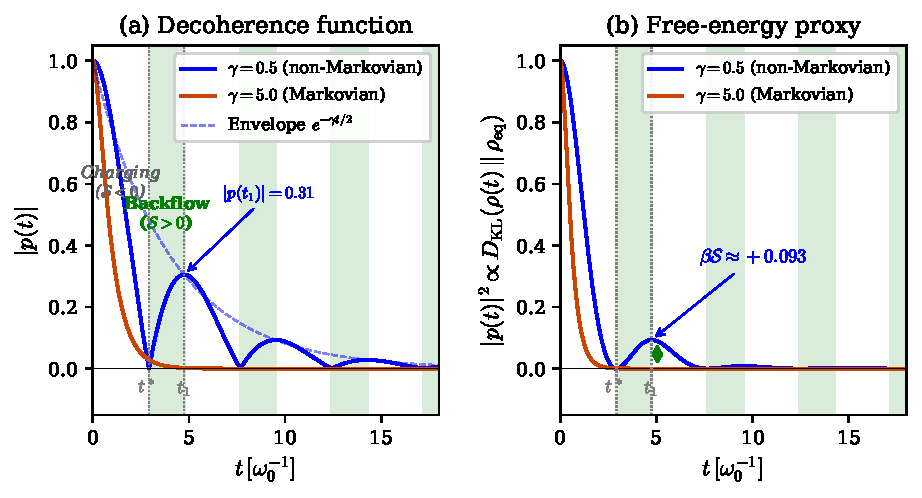
\includegraphics[width=\textwidth]{fig_survival.pdf}
\caption{%
Pure-dephasing spin-boson model
(Section~\ref{T-I-sec:example}) with Lorentz--Drude spectral
density~\eqref{T-I-eq:lorentz_drude}.
\textbf{Parameters:}
$\omega_0 = 1$ (energy unit),
$\lambda = 1$ (reorganization energy).
\textbf{Units:}
all times in $\omega_0^{-1}$;
energies in $\hbar\omega_0$.
\textbf{Regime:}
low temperature ($\beta\omega_0 \gg 1$);
the standard $T \to 0$ analytic
expression~\eqref{T-I-eq:decoherence}~\cite{BreuerPetruccione2002}
is used as an accurate proxy.
\textbf{(a)}~Decoherence amplitude $|p(t)|$
(eq.~\eqref{T-I-eq:decoherence}).
Blue: non-Markovian
($\gamma = 0.5$, $\gamma/4\lambda = 0.125$).
Orange: Markovian
($\gamma = 5.0$, $\gamma/4\lambda = 1.25$).
Dashed: exponential envelope $e^{-\gamma t/2}$.
Green bands indicate backflow
(Remark~\ref{T-I-rem:NM_regime}:
$d|p|/dt > 0$, $\Gamma(t) < 0$
per~\eqref{T-I-eq:Gamma_inst}).
\textbf{(b)}~Survival proxy
$|p(t)|^2 \propto \beta\,\mathcal{S}$
(eq.~\eqref{T-I-eq:S_qubit}).
At the first revival
($t_1 = \pi/\Omega \approx 4.75\,\omega_0^{-1}$),
the non-Markovian agent achieves
$\beta\,\mathcal{S}[t^*,t_1] \approx +0.093$
(eq.~\eqref{T-I-eq:S_numeric}), consistent with the
closed-form prediction~\eqref{T-I-eq:revival_exact},
funded by the consumption of pre-existing
correlations
(Proposition~\ref{T-I-prop:full_cycle}).
The Markovian comparison decays monotonically:
$\mathcal{S} \leq 0$ in this autonomous model
(Theorem~\ref{T-I-thm:autonomous_ceiling}).%
}
\label{T-I-fig:survival}
\end{figure}

\textbf{Consistency with
Theorem~\ref{T-I-thm:advantage} and
Proposition~\ref{T-I-prop:full_cycle}.}
Since this is autonomous evolution ($H_{\mathrm{ctrl}} = 0$),
identity~\eqref{T-I-eq:advantage_auto} applies exactly:
$\beta\,\mathcal{S} = -\Delta I(S{:}E)
- \Delta D_{\mathrm{KL}}(\rho_E \| \rho_E^{\mathrm{th}})$.
The example realizes the \emph{correlation battery}
of Remark~\ref{T-I-rem:battery}, with the charge--discharge
decomposition of
Proposition~\ref{T-I-prop:full_cycle}:
\begin{itemize}
\item \textbf{Charging} ($[0, t^*]$, eq.~\eqref{T-I-eq:charge}):
  the system decoheres, building correlations
  $I(S{:}E;\, t^*) > 0$ at the cost of
  $\mathcal{S} < 0$.
\item \textbf{Discharging} ($[t^*, t_1]$,
  eq.~\eqref{T-I-eq:discharge}):
  the correlations are consumed
  ($\Delta I < 0$ over this interval),
  returning $\beta\,\mathcal{S} \approx +0.093 > 0$.
\end{itemize}
The bound~\eqref{T-I-eq:S_upper} is satisfied:
$\beta\,\mathcal{S}[t^*, t_1] = 0.093
\leq I(S{:}E;\, t^*)$.
Full-cycle closure~\eqref{T-I-eq:full_cycle} is confirmed:
$\beta\,\mathcal{S}[0, t_1] < 0$.

\textbf{Instantaneous decoherence rate.}
The rate of coherence loss is
\begin{equation}
\label{T-I-eq:Gamma_inst}
\Gamma(t) := -\frac{d}{dt}\ln|p(t)|
= \frac{\gamma}{2}
  - \frac{\Omega\sin(\Omega t)
    + \tfrac{\gamma}{2}\cos(\Omega t)}
  {\cos(\Omega t)
    + \tfrac{\gamma}{2\Omega}\sin(\Omega t)}\,.
\end{equation}
In the Markovian limit $\gamma \gg 4\lambda$,
$\Gamma(t) \to \gamma/2 > 0$ for all $t$
(monotone decoherence).
In the non-Markovian regime $\gamma < 4\lambda$,
$\Gamma(t)$ oscillates and becomes \emph{negative}
during the backflow intervals where $|p(t)|$ increases.
These are precisely the intervals where
$\mathcal{S} > 0$.

\textbf{Closed-form revival amplitude.}
The decoherence function~\eqref{T-I-eq:decoherence} can be
written as $p(t) = R\, e^{-\gamma t/2}\cos(\Omega t - \phi)$,
where $R = \sqrt{1 + (\gamma/2\Omega)^2}$ and
$\phi = \arctan(\gamma/2\Omega)$, with $R\cos\phi = 1$.
The extrema of $|p(t)|$ occur at $t_n = n\pi/\Omega$
($n = 0, 1, 2, \ldots$), and the first revival peak
after the first zero is at $t_1 = \pi/\Omega$.
Its amplitude is \emph{exactly}
\begin{equation}
\label{T-I-eq:revival_exact}
|p(t_1)| = e^{-\gamma\pi/(2\Omega)},
\qquad
\beta\,\mathcal{S}[t^*, t_1]
\approx |p(t_1)|^2
= e^{-\gamma\pi/\Omega}.
\end{equation}
This is the paper's central computable prediction: the
survival gain at first backflow is determined by a single
dimensionless ratio $\gamma/\Omega$.

\begin{remark}[Parameter Survey]
\label{T-I-rem:parameter_survey}
Table~\ref{T-I-tab:survey} demonstrates the transition from
the Markovian regime ($\mathcal{S} \leq 0$) to the
non-Markovian regime ($\mathcal{S} > 0$) as the bath
memory rate $\gamma$ decreases below the critical value
$4\lambda$.
All entries use $\omega_0 = 1$, $\lambda = 1$,
$W = 0$ (autonomous evolution), with revival amplitudes
computed from~\eqref{T-I-eq:revival_exact}.
\begin{center}
\begin{tabular}{@{}cccccc@{}}
\toprule
$\gamma$ & $\gamma/4\lambda$ & Regime
& $|p(t_1)|$ & $\beta\,\mathcal{S}(t_1)$
& $\Gamma_{\min}$ \\
\midrule
$20.0$ & $5.0$ & Markov & --- & $\leq 0$ & $>0$ \\
$4.0$ & $1.0$ & Critical & --- & $\leq 0$ & $= 0$ \\
$2.0$ & $0.50$ & Non-Markov & $0.043$
  & $+0.002$ & $< 0$ \\
$1.0$ & $0.25$ & Non-Markov & $0.163$
  & $+0.027$ & $< 0$ \\
$0.5$ & $0.125$ & Deep NM & $0.305$
  & $+0.093$ & $< 0$ \\
$0.1$ & $0.025$ & Deep NM & $0.605$
  & $+0.37\phantom{0}$ & $< 0$ \\
\bottomrule
\end{tabular}
\end{center}
\captionsetup{hypcap=false}%
\captionof{table}{%
Survival functional at first backflow revival
as a function of the bath memory rate $\gamma$,
for the pure-dephasing spin-boson model
with Lorentz--Drude spectral density.
$|p(t_1)|$ is computed
from~\eqref{T-I-eq:revival_exact};
$\Gamma_{\min}$ is the sign of the minimum of the
instantaneous decoherence rate~\eqref{T-I-eq:Gamma_inst}.
The transition $\mathcal{S} \leq 0 \to \mathcal{S} > 0$
occurs precisely at the non-Markovian threshold
$\gamma = 4\lambda$.
For $\gamma = 0.1$ (deep non-Markovian),
the agent achieves $\beta\,\mathcal{S} \approx +0.37$
per backflow cycle in the autonomous setting
($H_{\mathrm{ctrl}} = 0$).%
}
\label{T-I-tab:survey}
\end{remark}

\begin{remark}[The Two Regimes: Summary]
\label{T-I-rem:two_regimes}
\begin{center}
\begin{tabular}{@{}lll@{}}
\toprule
& \textbf{Markovian ($\gamma = 20$)}
& \textbf{Non-Markovian ($\gamma = 0.5$)} \\
\midrule
$\gamma / 4\lambda$ & $5.0$ (overdamped)
  & $0.125$ (underdamped) \\
$\tau_B$ & $0.05\,\omega_0^{-1}$
  & $2.0\,\omega_0^{-1}$ \\
$p(t)$ & Monotone decay
  & Oscillatory with envelope \\
$|p(t_1)|$ at first revival & $0$ (no revival)
  & $\approx 0.31$ \\
$\beta\,\mathcal{S}$ at revival & $\leq 0$
  & $\approx +0.093$ \\
$\Gamma(t)$ & $> 0$ always
  & Oscillates, $< 0$ during backflow \\
Interpretation & Stone (sinks)
  & Surfer (rides backflow) \\
\bottomrule
\end{tabular}
\end{center}
The non-Markovian agent achieves
$\beta\,\mathcal{S} \approx +0.093$
per backflow cycle (autonomous, $H_{\mathrm{ctrl}} = 0$),
while the Markovian agent can only lose free energy.
As the coupling deepens ($\gamma/4\lambda \to 0$), the
revival amplitude grows and
$\mathcal{S}$ increases
(Table~\ref{T-I-tab:survey}), bounded above by
$\beta\,\mathcal{S} \leq I(S{:}E;\, t^*)$
(Corollary~\ref{T-I-cor:three_regimes}(iii)).
\end{remark}

% ============================================================
\section{The Cost of Memory}
\label{T-I-sec:cost}

The preceding identity allows a correlated initial resource to fund a
later interval.  It does not assign a universal energetic price to
storing or maintaining that resource.  This section separates
Landauer's erasure bound from a conditional archive-overload model used
only to motivate Paper~II.

\subsection{The Landauer Debt}

Landauer's principle prices a logically irreversible reset, not passive
storage, sensing, correlation maintenance, or reversible computation.

\begin{remark}[Conditional erasure cost]
\label{T-I-rem:landauer_scope}
If a declared memory implementation irreversibly erases
$N_{\mathrm{erase}}$ unbiased bits into a bath at temperature $T$, its
reset work obeys
\begin{equation}
\label{T-I-eq:landauer}
W_{\mathrm{reset}}\geq k_BT\ln2\,N_{\mathrm{erase}}.
\end{equation}
No lower bound proportional to total stored mutual information follows
without an implementation model.  Reversible storage and reversible
measurement can in principle avoid this reset cost until a logically
irreversible operation is performed~\cite{Landauer1961,Bennett1982}.
The former universal ``Landauer Cost of Memory'' proposition is
withdrawn.
\end{remark}

\subsection{Raw Archive Overload Scenario}

The crisis arises from the scaling of
$\mathcal{I}_{\mathrm{stored}}$ with time.
To quantify this, we borrow two quantities from computational
mechanics~\cite{CrutchfieldYoung1989,ShaliziCrutchfield2001}:

\begin{definition}[Entropy Rate and Predictive Information]
\label{T-I-def:entropy_rate}
Let $\{X_t\}$ be the stochastic process describing the
environment's influence on the agent (e.g., the sequence of
bath correlation values).
\begin{enumerate}
\item The \textbf{entropy rate} of the environment is
  \begin{equation}
  \label{T-I-eq:entropy_rate}
  h_\mu := \lim_{n \to \infty}
  H(X_n \mid X_{n-1}, \ldots, X_1),
  \end{equation}
  measuring the intrinsic unpredictability per time step.
\item The \textbf{predictive information} (excess entropy) is
  \begin{equation}
  \label{T-I-eq:pred_info}
  I_{\mathrm{pred}} := I(\overleftarrow{X};\,
  \overrightarrow{X})
  = \sum_{k=1}^{\infty}
  \bigl[H(X_k) - h_\mu\bigr],
  \end{equation}
  where $\overleftarrow{X}$ and $\overrightarrow{X}$ denote
  the past and future half-chains.
  This is the total amount of information about the future
  that is encoded in the past---the \emph{useful} memory.
\end{enumerate}
\end{definition}

Finite predictive information does not by itself prove that a finite
physical memory captures every useful feature, and positive entropy
rate does not lower-bound predictive information by
$h_\mu\tau_{\mathrm{mem}}$.  In particular, a stationary mixing
process commonly has finite excess entropy.

\begin{remark}[Conditional archive-overload scenario]
\label{T-I-rem:archive_overload}
Consider a deliberately specified implementation: an uncompressed raw
archive receives records at rate $r_{\mathrm{raw}}$ bits per unit time,
has capacity $M$ bits, and evaluates the entire archive once per control
cycle.  Without deletion it fills after $M/r_{\mathrm{raw}}$.  If it
irreversibly resets discarded records at rate $r_{\mathrm{erase}}$,
Landauer gives
\begin{equation}
\label{T-I-eq:mem_cost_rate}
\dot W_{\mathrm{reset}}\geq
k_BT\ln2\,r_{\mathrm{erase}}.
\end{equation}
For a long-memory or non-stationary source with divergent
$I_{\mathrm{pred}}$, the amount of predictively relevant history may
also grow, but that is an additional source assumption.  This archive
can exceed a finite storage, throughput, or reset budget.  The result is
an engineering overload scenario, not a universal thermodynamic
catastrophe and not a theorem that every memory implementation must
compress.
\end{remark}

\subsection{Conditional Motivation for Compression}

An agent using the raw-archive implementation may respond by increasing
capacity, lowering sample rate, reversible uncomputation, sufficient
statistics, lossy compression, or accepting stale data.  Paper~II
studies one coordinate-selection model among these options.

\begin{itemize}
\item \textbf{Compression requires a criterion.}
  To decide what to keep and what to erase, the agent needs a
  \emph{relevance function}---a mapping from stored correlations
  to survival value.
  This is a reference frame that ranks information by its
  contribution to $\mathcal{S}$.

\item \textbf{Coordinate selection uses a reference frame.}
  If the admissible compressor is restricted to retaining a subset of
  supplied coordinates, choosing that subset privileges a basis.  More
  general invariant or learned sufficient-statistic compressors need
  not have this form.
\end{itemize}

\begin{remark}[The Origin of Paper II]
\label{T-I-rem:paper_II}
Remark~\ref{T-I-rem:archive_overload} supplies Paper~II with a conditional
motivation: a bounded agent attempting to evaluate an uncompressed
archive needs some resource-allocation policy.  It does not prove that
compression, Clifford coordinates, spontaneous symmetry breaking, or a
``self'' is thermodynamically necessary.  Those are modelling choices
to be assessed in Paper~II.
\end{remark}

% ============================================================
\section{Numerical Demonstration}
\label{T-I-sec:numerical}

The preceding sections establish an autonomous thermodynamic baseline
and an accounting identity.  The following HMM is a separate classical
performance illustration: it compares finite observation windows with
a Bayes filter in an aliased environment.  Reward here is not the
thermodynamic survival functional, so the demonstration does not test
either theorem.
Full code and parameters are provided for reproducibility.

% ------------------------------------------------------------
\subsection{Model}
\label{T-I-subsec:demo_model}

\paragraph{Environment.}
A two-hidden-state HMM with aliased observations.
The hidden state $s_t \in \{0,1\}$ evolves as a persistent
Markov chain with $\Pr(s_{t+1} = s_t) = 1 - \varepsilon$;
the parameter $\varepsilon \in [10^{-3}, 10^{-1}]$ controls
the correlation length $\ell \sim 1/\varepsilon$.
Observations $o_t \in \{A, B\}$ are aliased:
$\Pr(o_t = A \mid s_t = 0) = 0.5 + \delta$,
$\Pr(o_t = A \mid s_t = 1) = 0.5 - \delta$,
with $\delta = 0.05$ (mutual information
$I(O; S) \approx 0.007$~bits).
Reward: $r_t = 1$ if $a_t = s_t$, $0$ otherwise.

\paragraph{Agents.}
All agents use the true model parameters and compute
exact Bayesian posteriors; the only difference is how many
observations each agent retains.
\begin{itemize}
\item \textbf{Markov-$k$} ($k \in \{1,2,4,8\}$): runs
  an exact Bayes filter over the most recent $k$
  observations (sliding window, uniform prior at each
  window start); acts by MAP.
\item \textbf{Memory (Bayes filter)}: maintains the full
  belief state $b_t = \Pr(s_t = 1 \mid o_{1:t})$ via the
  exact predict--update cycle over all past observations;
  acts by MAP.
\end{itemize}

\paragraph{Parameters.}
\begin{center}
\small
\begin{tabular}{@{}lcl@{}}
\toprule
\textbf{Quantity} & \textbf{Value} & \textbf{Role} \\
\midrule
$T$ & $100{,}000$ & horizon per trial \\
Seeds & 10 & independent replications \\
$\delta$ & 0.05 & observation asymmetry \\
$k$ & $\{1, 2, 4, 8\}$ & Markov window sizes \\
$\varepsilon$ & logspace($10^{-3}$, $10^{-1}$, 15)
  & transition noise grid \\
Burn-in & $5{,}000$ & discarded steps \\
\bottomrule
\end{tabular}
\end{center}

% ------------------------------------------------------------
\subsection{Results}
\label{T-I-subsec:demo_results}

Figure~\ref{T-I-fig:markov_ceiling} shows the two key signatures.

\paragraph{Result 1: finite-window performance saturation
(Figure~\ref{T-I-fig:markov_ceiling}a).}
The average reward $\bar{R}$ of the Bayes filter (memory
agent) increases monotonically with correlation length
$\ell = 1/\varepsilon$, while each Markov-$k$ agent
saturates at a distinct ceiling.  The ceilings are
ordered: $k = 1$ (lowest) through $k = 8$ (highest),
and all fall below the memory agent for
$\ell \gtrsim 20$.  This is a property of the specified
aliased HMM and agent classes, not a consequence of the
thermodynamic ceiling.

\paragraph{Result 2: Memory advantage
(Figure~\ref{T-I-fig:markov_ceiling}b).}
The gap $\Delta\bar{R} = \bar{R}_{\mathrm{mem}}
- \bar{R}_{\mathrm{Markov}\text{-}k}$ increases
monotonically with $\ell$, and is larger for smaller $k$.
Shaded bands show 95\% confidence intervals across
10 seeds.  The Markov-1 and Markov-2 curves nearly
overlap at small $\ell$, reflecting the fact that
short observation windows provide negligible additional
information in this aliasing regime---a consistency
check, not a deficiency.

\begin{figure}[t]
\centering
\includegraphics[width=\textwidth]%
  {fig_paper1_markov_ceiling.pdf}
\caption{%
\textbf{Finite-window saturation and Bayes-filter advantage.}
$T = 100{,}000$, 10 seeds, 95\% CI bands.
\textbf{(a)}~Average reward $\bar{R}$ vs correlation
length $\ell = 1/\varepsilon$.  The Bayes filter
(blue, bold) rises monotonically; Markov-$k$ agents
saturate at $k$-dependent ceilings.
\textbf{(b)}~Performance gap
$\Delta\bar{R} = \bar{R}_{\mathrm{mem}}
- \bar{R}_{\mathrm{Markov}\text{-}k}$
increases with $\ell$; smaller $k$ yields a larger gap.}
\label{T-I-fig:markov_ceiling}
\end{figure}

% ------------------------------------------------------------
\subsection{Scope of This Demonstration}
\label{T-I-subsec:demo_scope}

These simulations illustrate finite-window saturation under the stated
model class; they do not constitute a thermodynamic test.

\medskip
This demonstration \textbf{does} show:
\begin{enumerate}
\item A reproducible regime in which finite-order Markov
  agents exhibit a performance ceiling while a
  memory-carrying (Bayes filter) agent improves.
\item The performance gap widens with correlation length and tightens
  with window size in this HMM.  This is conceptually related to
  retained history but is not the quantity in
  Theorem~\ref{T-I-thm:advantage}.
\end{enumerate}

\noindent
This demonstration does \textbf{not} show:
\begin{enumerate}
\item Universality across environments, observation models,
  or agent architectures.  The model uses a two-state
  HMM with binary aliased observations.
\item Tight constants or the functional form of the
  ceiling boundary $\ell_c(k)$.
\item That the Bayes filter is optimal among all possible
  memory-carrying agents.
\end{enumerate}

\paragraph{Reproducibility.}
\begin{sloppypar}
The complete simulation is a self-contained Python script
(\texttt{paper1\_markov\_ceiling\_demo.py}, ${\sim}\,560$
lines, requiring only NumPy and Matplotlib) with fixed
random seeds.  All figures in this section can be
reproduced by executing the script.  The following files
are included in the supplementary archive:
\begin{itemize}
\item \texttt{paper1\_markov\_ceiling\_demo.py} --- simulation script
\item \texttt{fig\_paper1\_markov\_ceiling.pdf} --- Figure~\ref{T-I-fig:markov_ceiling}
\item \texttt{markov\_ceiling\_data.csv} --- raw sweep data
\item \texttt{markov\_ceiling\_boundary.csv} --- extracted
  ceiling boundaries $\ell_c(k)$
\end{itemize}
\end{sloppypar}

% ============================================================
\section{Discussion}
\label{T-I-sec:discussion}

\subsection{Summary of Results}

\begin{center}
\small
\setlength{\tabcolsep}{4pt}%
\begin{tabular}{@{}lP{7.5cm}c@{}}
\toprule
\textbf{Result} & \textbf{Statement} & \textbf{Sec.} \\
\midrule
Restricted autonomous ceiling &
  $\mathcal{S} \leq 0$ for a fixed-Hamiltonian Davies semigroup
  & \ref{T-I-sec:ceiling} \\[3pt]
Initial-resource balance &
  $\beta\mathcal{S} = -\Delta I
  - \Delta D_{\mathrm{KL}}
  - \beta\Delta\langle H_{\mathrm{ctrl}}\rangle
  - \beta\Delta\langle H_{\mathrm{int}}\rangle$
  & \ref{T-I-sec:advantage} \\[3pt]
Quantitative demo &
  Spin-boson: $\beta\mathcal{S} \approx +0.093 > 0$
  at first backflow revival (Fig.~\ref{T-I-fig:survival},
  Table~\ref{T-I-tab:survey})
  & \ref{T-I-sec:example} \\[3pt]
Memory/record interface &
  operational influence relation plus a conditional record test
  & \ref{T-I-sec:arrow} \\[3pt]
Archive overload &
  conditional on raw storage, finite capacity, and irreversible reset
  & \ref{T-I-sec:cost} \\[3pt]
Numerical demo &
  finite-window saturation in an aliased HMM
  (Fig.~\ref{T-I-fig:markov_ceiling})
  & \ref{T-I-sec:numerical} \\
\bottomrule
\end{tabular}
\end{center}

\subsection{What This Paper Does and Does Not Show}

\textbf{This paper shows:}
\begin{enumerate}
\item Under an autonomous fixed-Hamiltonian Davies semigroup,
  the survival functional $\mathcal{S} \leq 0$
  (Theorem~\ref{T-I-thm:autonomous_ceiling}).
\item For any initial state (product or correlated), the
  survival functional satisfies the exact identity
  $\beta\,\mathcal{S} = -\Delta I(S{:}E)
  - \Delta D_{\mathrm{KL}}(\rho_E \| \rho_E^{\mathrm{th}})
  - \beta\,\Delta\langle H_{\mathrm{ctrl}}\rangle
  - \beta\,\Delta\langle H_{\mathrm{int}}\rangle$
  (Theorem~\ref{T-I-thm:advantage}).
  Under autonomous evolution, when pre-existing
  system--environment correlations are consumed
  ($\Delta I < 0$), $\mathcal{S} > 0$ is achievable,
  bounded by the initial correlation budget
  (Corollary~\ref{T-I-cor:three_regimes}).
\item A quantitative spin-boson example illustrates:
  $\beta\,\mathcal{S} \approx +0.093 > 0$ at the first
  non-Markovian revival (Section~\ref{T-I-sec:example}).
\item The memory-influence relation and HAFF record ordering define a
  conditional model test, not a proved embedding
  (Conjecture~\ref{T-I-prop:HAFF_bridge}).
\item Landauer supplies a conditional reset cost; a raw finite archive
  can overload under the implementation assumptions in
  Remark~\ref{T-I-rem:archive_overload}.
\item A computational demonstration exhibits finite-window saturation
  in a two-state HMM with aliased observations
  (Section~\ref{T-I-sec:numerical},
  Figure~\ref{T-I-fig:markov_ceiling}).
\end{enumerate}

\textbf{This paper does not show:}
\begin{enumerate}
\item That memory or non-Markovianity is necessary or sufficient for
  persistence.
\item That non-Markovian systems optimize a larger survival supremum
  than all Markovian systems.
\item That driven or measurement-feedback Markovian agents obey the
  restricted autonomous ceiling (Remark~\ref{T-I-rem:driven_protocol}).
\item That the specific form of the optimal memory kernel can be
  derived from first principles without specifying the
  environment.
\item That memory implies or requires consciousness.
\item That storage or maintenance has a universal Landauer cost, or
  that compression and symmetry breaking are thermodynamic necessities.
\end{enumerate}

% ============================================================
% REFERENCES
% ============================================================

% ============================================================================
% Paper II --- ``The Ego''
% ============================================================================
\chapter{Spontaneous Symmetry Breaking of Reference Frames as a Computational Cost Minimization Strategy}
\label{T-chap:paperII}

\begin{center}
\textit{Paper II --- ``The Ego''}\\[0.5em]
Originally published: Zenodo, DOI: 10.5281/zenodo.18579703
\end{center}

\bigskip

\section*{Abstract}
We investigate a conditional implementation model for bounded agents
that process memory-like state under finite computational resources.
Revised Paper~I~\cite{Liu2026TDOME_I} supplies a conditional
correlation-resource account; it does not establish universal memory
necessity, a universal Markovian ceiling, or a Landauer charge for
merely storing records.

The present paper therefore studies a declared raw $D$-channel archive
processed under a finite throughput budget.  Within that model,
symmetric processing of all declared channels can exceed the available
budget at a finite time, while a supplied coordinate selector can reduce
the declared load.  This is a conditional overload result for the stated
archive and algorithm, not a theorem that every persistent agent must
compress memory or break a symmetry.

Reference-frame selection is treated as a modelling strategy: a
privileged basis or coordinate projection packages a lower-dimensional
representation of the archive.  The rate-distortion calculation gives a
budget-dependent target dimension under the stated source, distortion,
and budget assumptions.  It does not prove that the ``self'' is a
universal survival-optimal structure.

The projected representation is accompanied by four diagnostic labels:
basis selection, frame drag, objective centering, and model
incompleteness.  Only basis selection follows from projection alone; the
other diagnostics require additional controller, update, objective, or
task assumptions.  A simple drift model gives a visibility crossover for
a fixed frame, motivating Paper~III's calibration problem without
establishing an undetectable universal Delusion Trap.


% ============================================================
\section{Introduction}
\label{T-II-sec:intro}

% ------------------------------------------------------------
\subsection{Context: The Problem of Overload}
\label{T-II-subsec:overload}

Revised Paper~I~\cite{Liu2026TDOME_I} gives an ELV-type
accounting identity in which initial correlations can fund a later
interval and proves a ceiling only for a fixed-Hamiltonian autonomous
Davies baseline.  It retracts both universal memory necessity and a
Landauer charge for merely storing or maintaining records.

The present paper therefore begins with an independent implementation
model: a raw, uncompressed $D$-channel archive processed under a finite
throughput budget.  Its overload is conditional on that archive and
algorithm.  The question is when a supplied coordinate selector can
reduce this declared load, not whether every persistent agent must
compress or break symmetry.

% ------------------------------------------------------------
\subsection{Position within the Series}
\label{T-II-subsec:series_position}

This paper is the second of three constituting the
\textbf{T-DOME} (Thermodynamic Dynamics of Observer-Memory
Entanglement) framework, the third pillar of a three-paper
program.

\begin{center}
\small
\setlength{\tabcolsep}{4pt}%
\begin{tabular}{@{}lP{3.2cm}cP{3.4cm}c@{}}
\toprule
\textbf{Framework} & \textbf{Question} & & \textbf{Result}
  & \textbf{Status} \\
\midrule
HAFF~\cite{Liu2026HAFF_A,Liu2026HAFF_B}
  & How does geometry emerge?
  & Ocean
  & Conditional algebra/dictionary models
  & Revised \\[3pt]
Q-RAIF~\cite{Liu2026QRAIF_A,Liu2026QRAIF_B}
  & What algebra must an observer have?
  & Fish
  & Clifford representation as model input
  & Revised \\[3pt]
T-DOME~I~\cite{Liu2026TDOME_I}
  & What can inter-epoch correlations fund?
  & Seed
  & Restricted baseline; accounting identity
  & Conditional \\[3pt]
\textbf{T-DOME~II} (this work)
  & When can a model select a frame?
  & Ego
  & Conditional coordinate selection
  & \textbf{This paper} \\[3pt]
T-DOME~III
  & When can residual statistics track drift?
  & Loop
  & Conditional Fisher calibration
  & Companion \\
\bottomrule
\end{tabular}
\end{center}

The three T-DOME papers form a conditional modelling sequence rather
than an irreversible theorem chain:
\begin{enumerate}
\item \textbf{Paper~I (The Seed):} An ELV-type balance identifies
  initial correlations as one possible interval resource.  Raw-archive
  overload is an implementation scenario, not a thermodynamic
  necessity.
\item \textbf{Paper~II (The Ego, this work):} Unbounded memory
  under finite computational resources causes processing
  overload in the coordinate-processing model.  This paper studies
  conditional feature selection; it does not prove universal SSB.
\item \textbf{Paper~III (The Loop):} Uncorrected bias diverges
  from a changing environment. A self-referential calibration
  loop (monitoring one's own prediction error) resolves the
  bias but requires the system to ``observe its own
  observation''---closing the self-calibration loop.
\end{enumerate}

% ------------------------------------------------------------
\subsection{Relation to Q-RAIF}
\label{T-II-subsec:qraif}

Revised Q-RAIF Papers A and B~\cite{Liu2026QRAIF_A,Liu2026QRAIF_B}
use a Clifford algebra $Cl(V,q)$ as a supplied representation choice;
persistence does not select it.  Paper C~\cite{Liu2026QRAIF_C} proves
only that the image of a separately supplied homomorphism lies in the
external algebra.  This paper adopts both the Clifford coordinates and
the representation map as model inputs.

The Clifford algebra $Cl(V,q)$, however, admits a non-trivial
\emph{automorphism group} $G = \mathrm{Aut}(Cl(V,q))$.
In the absence of external constraints, all elements of $G$
yield physically equivalent representations---the choice of
basis within the algebra is a \emph{gauge freedom}.
This gauge freedom is the mathematical substrate of the
symmetry considered in the conditional breaking analysis below.

The ``ego'' names a selected computational frame in that supplied
representation.  Whether a concrete optimum is a genuine gauge fixing
is a model condition, not an inherited theorem.

% ------------------------------------------------------------
\subsection{Relation to HAFF Paper~G}
\label{T-II-subsec:haff_g}

Revised HAFF Paper~G~\cite{Liu2026HAFF_G} offers
philosophy-of-science motivation and no fixed-point no-go theorem.  It
does not imply basis selection here.  Any connection between its
meta-level concern and this finite-budget model is motivation only.

% ------------------------------------------------------------
\subsection{Scope and Disclaimers}
\label{T-II-subsec:scope}

To prevent interpretational overreach, we state at the
outset what this paper does \emph{not} claim:
\begin{enumerate}
\item We do not claim that symmetry breaking is
  \emph{sufficient} for persistence.
  Paper~III addresses the additional requirements.
\item We do not claim that basis selection or spontaneous symmetry
  breaking is necessary for every bounded agent.  The results concern
  a declared coordinate-retention model.
\item The term ``ego'' or ``self'' is used in the
  control-theoretic sense: a fixed reference frame within
  the agent's internal algebra. It carries no implication
  of consciousness or subjective experience.
\item A broader structural analogy with classical philosophical
  concepts of selfhood exists but is outside the scope of
  this paper.
\end{enumerate}

\paragraph{Related work.}
The idea that bounded agents must compress their
representations has roots in Simon's bounded
rationality~\cite{Simon1955}, Shannon's
rate-distortion theory~\cite{Shannon1959,CoverThomas2006},
and Sims's rational inattention~\cite{Sims2003}, which
models finite-capacity decision-makers as solving a
rate-distortion problem---precisely the economic
counterpart of our $\mathcal{C}_{\mathrm{budget}}$
formalism.
The information bottleneck~\cite{Tishby2000}
formalises relevance-weighted compression and has been
applied to neural coding and deep
learning.
The role of decoherence in selecting preferred bases
(pointer states) is well established via quantum
Darwinism~\cite{Zurek2009}; here it motivates one
model-specific coordinate-selection rule.
Measures of non-Markovianity and their thermodynamic
consequences are reviewed
in~\cite{RivasHuelgaPlenio2014,BreuerPetruccione2002};
the connection to survival was established in Paper~I.

\paragraph{Summary of contributions.}
This paper separates three levels of result:
\begin{enumerate}
\item \textbf{Raw-channel load scaling law}
  a conditional accounting identity for a raw $D$-channel archive.
\item \textbf{Survival-weighted rate-distortion bound}
  a compactness-based existence result; the budget supplies only a
  capacity $k_{\max}$, not a universal optimal retained dimension.
\item \textbf{Delusion dynamics}
  a linear-drift visibility crossover plus an explicit two-mode
  example showing when gradient anti-correlation can occur.
\end{enumerate}

\paragraph{Result-status ledger.}
The original Computational Ceiling and SSB-necessity chain is retracted
(`TD-II-T3.5`).  Raw-channel load is an FD/I accounting proposition;
compression existence is conditional on a compact feasible model; SSB
is a model interpretation.  The Delusion Trap is downgraded
(`TD-II-T6.7`): visibility crossover is exact in the declared two-mode
geometry, while gradient sign and self-detection require extra dynamics.

% ============================================================
\section{Mathematical Preliminaries}
\label{T-II-sec:prelim}

% ------------------------------------------------------------
\subsection{Inherited Framework from Paper~I}
\label{T-II-subsec:inherited}

We briefly recall the key objects from
Paper~I~\cite{Liu2026TDOME_I} that the present work builds
upon.  The reader is referred to Paper~I for full definitions
and proofs.

\paragraph{Survival functional.}
For an open quantum system $S$ coupled to an environment $E$
at inverse temperature $\beta$, with dynamics $\Lambda$ and
external control protocol $H_{\mathrm{ctrl}}(t)$, the
survival functional is
\begin{equation}
\label{T-II-eq:survival_recall}
\mathcal{S}[\Lambda, \tau]
:= \Delta F - W[0,\tau],
\end{equation}
where $\Delta F = F(\rho(\tau)) - F(\rho(0))$ is the change
in non-equilibrium free energy and
$W = \int_0^\tau \tr(\rho(t)\,\dot{H}_{\mathrm{ctrl}}(t))\,dt$
is the work performed by the external protocol.

\paragraph{Restricted autonomous baseline.}
For a fixed-Hamiltonian Davies semigroup with no control, Paper~I proves
\begin{equation}
\label{T-II-eq:ceiling_recall}
\mathcal{S}[\Lambda^{\mathrm{M}}, \tau] \leq 0
\qquad\text{for all } \tau \geq 0.
\end{equation}
It does not extend this result to driven Markovian agents.

\paragraph{Non-Markovian advantage identity.}
For arbitrary initial states:
\begin{equation}
\label{T-II-eq:advantage_recall}
\beta\,\mathcal{S}
= -\Delta I(S{:}E)
  - \Delta D_{\mathrm{KL}}(\rho_E \| \rho_E^{\mathrm{th}})
  - \beta\,\Delta\langle H_{\mathrm{ctrl}} \rangle
  - \beta\,\Delta\langle H_{\mathrm{int}} \rangle.
\end{equation}

\paragraph{Conditional raw-archive model.}
Paper~I retracts a universal Landauer maintenance bound.  This paper
independently posits an uncompressed record stream.  Let $h_\mu$ be its
\emph{per-component} entropy rate~\cite{CrutchfieldYoung1989},
defined by
\begin{equation}
\label{T-II-eq:entropy_rate}
h_\mu
:= \lim_{T\to\infty}\frac{1}{T}\,H(X_{0:T}),
\end{equation}
measuring the asymptotic information (in bits per unit time)
generated by one declared record channel (we work in units where the sampling interval equals
the environmental correlation time
$\tau_E$)\footnote{For a continuous-valued process sampled at
resolution $b$ bits, $h_\mu$ includes the quantisation cost:
$h_\mu = h_\mu^{(\mathrm{diff})} + b\,f_s$, where
$h_\mu^{(\mathrm{diff})}$ is the differential entropy rate
and $f_s$ the sampling frequency.  All raw-channel accounting
identities in this paper use $h_\mu$ so defined.}
The predictive information
$I_{\mathrm{pred}}$ is the \emph{excess entropy}
(excess entropy)~\cite{BialekNemenmanTishby2001,ShaliziCrutchfield2001},
defined as the mutual information between past and future
of the environmental process:
\begin{equation}
\label{T-II-eq:I_pred}
I_{\mathrm{pred}}
:= I\!\left(\overleftarrow{X};\, \overrightarrow{X}\right)
= H(\overrightarrow{X})
  - H(\overrightarrow{X} \mid \overleftarrow{X}),
\end{equation}
where $\overleftarrow{X}$ and $\overrightarrow{X}$ denote
the semi-infinite past and future, respectively.
For a stationary process,
$I_{\mathrm{pred}}$ relates to $h_\mu$ via the entropy-rate
decomposition
$H(X_{1:T}) = I_{\mathrm{pred}} + h_\mu\,T + o(1)$
as $T \to \infty$ when the relevant limits exist
\cite{CrutchfieldYoung1989}.  No lower bound
$I_{\mathrm{stored}}\geq\min(I_{\mathrm{pred}},h_\mu\tau)$
is inherited.

% ------------------------------------------------------------
\subsection{The Agent's Internal Algebra}
\label{T-II-subsec:algebra}

As a modelling choice motivated by revised
Q-RAIF~\cite{Liu2026QRAIF_B,Liu2026QRAIF_C},
the agent's internal control algebra is taken to be a Clifford algebra
$\mathcal{O}_{\mathrm{int}} = Cl(V,q)$
for a real vector space $V$ equipped with a non-degenerate
quadratic form $q$.
The algebra satisfies the fundamental relation
$v^2 = q(v)\,\mathbf{1}$ for all $v \in V$.

The \emph{automorphism group}
\begin{equation}
\label{T-II-eq:gauge_group}
G := \mathrm{Aut}(Cl(V,q))
\end{equation}
is the group of algebra automorphisms that preserve the
grading and quadratic form.\footnote{\label{T-II-fn:gauge_group}%
We use $G$ as an effective symmetry group acting
transitively on admissible frames.
The detailed Lie-algebraic structure of $G$ is not required
for our results; only the existence of a non-trivial
symmetry that may be broken under the additional encoder
conditions in Remark~\ref{T-II-rem:conditional_ssb}.
In concrete models, one may replace $G$ by its image
under the adjoint representation---typically
$O(V,q)$ or a pin/spin subgroup.}
For $Cl(1,3)$, $G$ contains the spin group
$\mathrm{Spin}(1,3) \cong SL(2,\mathbb{C})$
as a subgroup---a six-real-dimensional Lie group.

In the absence of computational constraints, all
$g \in G$ yield physically equivalent descriptions of
the agent's internal state.
The choice of basis within $Cl(V,q)$ is a \emph{gauge
freedom}---the symmetry examined in the conditional
coordinate-selection model below.

A representation map
$\phi:Cl(V,q)\to\mathcal A_{\mathrm{ext}}$ is supplied as an
interface.  Q-RAIF Paper C proves only the image-level algebraic
statement once this map is given; it does not select a preferred
$Cl(1,3)$ target or preserve quadratic signature.

\paragraph{Dimensional convention.}
Two distinct notions of dimension appear throughout:
\begin{center}
\small
\begin{tabular}{@{}lll@{}}
\toprule
Symbol & Meaning & Scaling \\
\midrule
$n := \dim V$ & number of generators
  (degrees of freedom) & --- \\
$D := \dim Cl(V,q) = 2^n$ & full multivector space
  (algebra basis size) & exponential in $n$ \\
\bottomrule
\end{tabular}
\end{center}
The raw-channel load model (Section~\ref{T-II-sec:ceiling})
scales with~$D$, not~$n$; the distinction matters
whenever one compares generator-level and
algebra-level quantities.

% ------------------------------------------------------------
\subsection{Rate-Distortion Theory}
\label{T-II-subsec:RD}

We require the classical rate-distortion framework
of Shannon~\cite{Shannon1959}.

\begin{definition}[Rate-distortion function]
\label{T-II-def:RD}
Let $X$ be a random source with distribution $p(x)$,
$\hat{X}$ a reconstruction, and
$d: \mathcal{X} \times \hat{\mathcal{X}} \to [0,\infty)$
a distortion measure.
The \emph{rate-distortion function} is
\begin{equation}
\label{T-II-eq:RD}
R(D) := \min_{\substack{p(\hat{x}|x):\\
  \mathbb{E}[d(X,\hat{X})] \leq D}} I(X; \hat{X}),
\end{equation}
the minimum mutual information between source and
reconstruction that achieves average distortion at most $D$.
\end{definition}

$R(D)$ is a convex, non-increasing function of $D$ with
$R(0) = H(X)$ (lossless) and
$R(D_{\max}) = 0$ (maximum distortion).
It provides the fundamental limit on lossy
compression~\cite{CoverThomas2006}.
The \emph{information bottleneck} method of
Tishby et al.~\cite{Tishby2000} generalises this framework
to the case where the relevant variable is not the source
itself but a downstream prediction target---precisely the
situation in our survival-weighted compression problem
(Section~\ref{T-II-subsec:RD_bound}).
For source $X$, representation $Z$, and declared survival-relevant
target $Y$, the bottleneck objective is
\begin{equation}
\min_{p(z|x)} I(X;Z)-\beta_{\mathrm{IB}} I(Z;Y).
\end{equation}
The coordinate-retention model below does not solve this unrestricted
optimization.  Rate-distortion and information bottleneck therefore
provide comparison frameworks, not authority for the component count.

% ------------------------------------------------------------
\subsection{Bounded Rationality}
\label{T-II-subsec:bounded}

Following Simon~\cite{Simon1955}, we model computational
limitations as a hard constraint on the agent's information
processing rate.

\begin{definition}[Computational budget]
\label{T-II-def:budget}
The agent's \emph{computational budget}
$\mathcal{C}_{\mathrm{budget}}$ (measured in bits per unit
time) is the maximum rate at which the agent can evaluate
functions of its stored correlations.
We assume $\mathcal{C}_{\mathrm{budget}} < \infty$.
\end{definition}

Physically, finiteness of $\mathcal{C}_{\mathrm{budget}}$
reflects the finite number of degrees of freedom in the
agent's physical substrate: finite Hilbert space dimension,
finite memory register size, and finite energy available for
computation (Landauer's
principle~\cite{Landauer1961,Bennett1982}).

% ------------------------------------------------------------
\subsection{Fiber Bundle Formalism}
\label{T-II-subsec:fiber}

The geometric setting for reference-frame selection is a
principal fiber bundle.

\begin{definition}[Gauge bundle]
\label{T-II-def:bundle}
The \emph{gauge bundle} is the principal $G$-bundle
\begin{equation}
\label{T-II-eq:bundle}
\pi: P \to M, \qquad G = \mathrm{Aut}(Cl(V,q)),
\end{equation}
where:
\begin{itemize}
\item $M$ is the base space of \emph{effective memory
  kernels}---equivalently, the space of induced
  sufficient-statistic processes accessible to the agent
  (a finite-dimensional manifold that admits local
  parametrisation by the environmental spectral-density
  couplings);
\item $G$ is the structure group acting transitively on
  admissible frames (see
  footnote~\ref{T-II-fn:gauge_group} for the effective
  subgroup);
\item the fiber $\pi^{-1}(\kappa)$ over a kernel
  $\kappa \in M$ is the $G$-orbit of equivalent algebraic
  representations (frames) for describing~$\kappa$
  in $Cl(V,q)$;
\item a \emph{section} $\sigma: M \to P$ constitutes a
  global gauge-fixing policy---a systematic choice
  of reference frame for every kernel configuration.
\end{itemize}
\end{definition}

A \emph{connection} on $P$ specifies how the reference frame
is parallel-transported as the agent's state evolves.
The curvature of this connection measures the extent to
which the reference frame ``twists'' along different paths
through state space.

% ------------------------------------------------------------
\subsection{Standing Assumptions}
\label{T-II-subsec:standing}

\begin{definition}[Standing Assumptions]
\label{T-II-def:assumptions_B}
Throughout this paper, the following conditions are assumed:
\begin{enumerate}
\item[\textup{(B1)}] \textbf{Inherited framework.}
  All assumptions (A1)--(A5) of
  Paper~I~\cite{Liu2026TDOME_I} remain in force
  (open quantum system coupled to a thermal bath,
  well-defined free energy, non-equilibrium initial state,
  finite-dimensional system Hilbert space,
  and weak-coupling or controlled-coupling regime).
  Additionally, the agent possesses an internal control
  algebra $\mathcal{O}_{\mathrm{int}} = Cl(V,q)$
  with a supplied representation map
  $\phi:Cl(V,q)\to\mathcal A_{\mathrm{ext}}$
  (Q-RAIF~\cite{Liu2026QRAIF_C}).  Neither the Clifford choice nor
  the map is derived from persistence.
\item[\textup{(B2)}] \textbf{Finite computational budget.}
  The agent's information processing rate satisfies
  $\mathcal{C}_{\mathrm{budget}} < \infty$
  (Definition~\ref{T-II-def:budget}).
\item[\textup{(B3)}] \textbf{Raw-channel load model.}
  The supplied record process has $D$ declared component channels,
  per-channel innovation rate $h_\mu>0$, memory depth
  $\tau_{\mathrm{mem}}>0$, and no shared-code or group-theoretic
  compression before the accounting in Section~\ref{T-II-sec:ceiling}.
  This worst-case assumption, not environmental non-triviality alone,
  carries the load calculation.
\item[\textup{(B4)}] \textbf{Survival imperative.}
  The agent's dynamics must maintain
  $\mathcal{S} \geq \mathcal{S}_{\min}$
  over survival horizons
  $T \gg \tau_{\mathrm{mem}}$.
  This is a persistence constraint, not an optimization
  objective.
\item[\textup{(B5)}] \textbf{Gauge symmetry of bare
  algebra.}
  The automorphism group $G = \mathrm{Aut}(Cl(V,q))$
  is non-trivial ($G \neq \{e\}$).
  In the absence of computational constraints, all
  $g \in G$ yield physically equivalent descriptions.
\end{enumerate}
\end{definition}

% ============================================================
\section{Raw-Channel Load Model}
\label{T-II-sec:ceiling}

We now record the throughput of the raw-channel model in (B3).  This is
a bookkeeping identity for an explicitly compression-free
representation, not a lower bound over all symmetric algorithms and not
a consequence of Paper~I.

% ------------------------------------------------------------
\subsection{The Information Processing Inequality
for Bounded Agents}
\label{T-II-subsec:processing}

\paragraph{Accounting convention.}
To ensure dimensional consistency throughout, we distinguish
two quantities:
\begin{itemize}
\item $\mathcal{C}_{\mathrm{budget}}$: the agent's processing
  \emph{rate} (bits per unit time).
\item $\mathcal{I}_{\mathrm{proc}}(\tau)$: the total
  information (bits) that must be processed per evaluation
  cycle when the memory archive has depth $\tau$.
\end{itemize}
The agent must complete one evaluation cycle per
environmental correlation time $\tau_E$.
The \emph{processing rate} required for a memory depth
$\tau$ is
\begin{equation}
\label{T-II-eq:rate_def}
\mathcal{R}_{\mathrm{proc}}(\tau)
:= \frac{\mathcal{I}_{\mathrm{proc}}(\tau)}
        {\tau_E}.
\end{equation}
Paralysis occurs when
$\mathcal{R}_{\mathrm{proc}}(\tau_{\mathrm{mem}})
> \mathcal{C}_{\mathrm{budget}}$.
Hereafter we measure time in units of $\tau_E$
(i.e., set $\tau_E = 1$), so that rates and per-cycle
information quantities are numerically equal.

\begin{definition}[Symmetric processing]
\label{T-II-def:symmetric}
An agent processes its memory \emph{symmetrically} if both
its cost functional $\mathcal{C}[\cdot]$ and its distortion
measure $D(\cdot)$ are $G$-invariant:
$\mathcal{C}[g \cdot \mathcal{K}]
= \mathcal{C}[\mathcal{K}]$ and
$D(g \cdot \mathcal{F}) = D(\mathcal{F})$
for every $g \in G = \mathrm{Aut}(Cl(V,q))$.
In operational terms: for every stored correlation $c_i$ in the
memory kernel $\mathcal{K}(t,s)$ and every $g \in G$, the
cost of evaluating $c_i$ equals the cost of evaluating
$g \cdot c_i$, and no basis direction is
\emph{a priori} preferred for survival evaluation.
\end{definition}

\begin{remark}[Operational meaning of processing rate]
\label{T-II-rem:proc_rate}
We define the processing rate
$\mathcal{R}_{\mathrm{proc}}$ as an
\emph{information-throughput} measure: the number of
algebraic components that must be updated per unit time,
multiplied by the innovation rate $h_\mu$ per component.
It captures the \emph{bandwidth} cost of maintaining an
internal representation, not the algorithmic gate
complexity of individual operations.
\end{remark}

\begin{proposition}[Raw-channel load accounting]
\label{T-II-prop:raw_load}
Under (B3), let $n=\dim V$ and
$D=\dim Cl(V,q)=2^n$.  A raw archive of depth
$\tau_{\mathrm{mem}}$ contains, by the model definition,
\begin{equation}
\label{T-II-eq:comp_ceiling}
\mathcal I_{\mathrm{archive}}
=D\,h_\mu\,\tau_{\mathrm{mem}}
\qquad\text{bits}.
\end{equation}
Its incremental input rate is $D h_\mu$ bits per unit time.  If the
declared algorithm rescans the entire archive once per environmental
correlation time $\tau_E$, its required throughput is
\begin{equation}
\label{T-II-eq:paralysis}
\mathcal R_{\mathrm{sweep}}
=\frac{D h_\mu\tau_{\mathrm{mem}}}{\tau_E}.
\end{equation}
For a processing budget $\mathcal C_{\mathrm{budget}}$, this particular
full-sweep algorithm fits only when
\begin{equation}
\label{T-II-eq:t_par}
\tau_{\mathrm{mem}}\leq
\tau_{\max}:=
\frac{\mathcal C_{\mathrm{budget}}\tau_E}{D h_\mu}.
\end{equation}
\end{proposition}

\begin{proof}
All three statements follow by multiplying the declared number of
channels by their per-channel innovation rate and then converting stored
bits per sweep to bits per unit time.  No lower bound over compressed,
streaming, sufficient-statistic, or group-equivariant algorithms is
claimed.
\end{proof}

\begin{remark}[Conditional component-count ratio]
\label{T-II-rem:symmetry_tax}
Within the same raw-coordinate implementation, comparing a $D$-channel
sweep with a $k$-channel sweep gives the component-count ratio $D/k$.
This is not a tax imposed by gauge invariance on all algorithms.
\end{remark}

\begin{remark}[Effective vs.\ full dimension]
\label{T-II-rem:D_eff}
The ceiling uses $D = \dim Cl(V,q) = 2^n$, the full
multivector dimension.
In practice, the environment may couple to only a subset of
grades (e.g., grade-1 generators), yielding an effective
dimension $D_{\mathrm{eff}} \leq D$.
For a \emph{structured} environment where the agent knows
which grades are active, the ceiling can be tightened to
$\mathcal{R}_{\mathrm{proc}} \gtrsim h_\mu
\cdot D_{\mathrm{eff}}$.
The raw-channel condition in (B3) represents this worst case.  A
structured environment or algorithm changes the model rather than
falling under a universal ceiling.
\end{remark}

% ------------------------------------------------------------
\subsection{Processing Collapse}
\label{T-II-subsec:collapse}

\begin{remark}[Raw full-sweep overload]
\label{T-II-rem:raw_overload}
If $\tau_{\mathrm{mem}}>\tau_{\max}$, the full-sweep algorithm in
Proposition~\ref{T-II-prop:raw_load} misses its declared cycle deadline.
This does not imply that every record is useless or that another
streaming/compressed algorithm fails.
\end{remark}

\begin{remark}[Comparison with revised Paper~I]
\label{T-II-rem:comparison}
Paper~I now treats storage/reset cost as implementation-dependent.  The
present overload is likewise conditional on a raw full-sweep algorithm.
Compression is one response; neither paper proves it must take the form
of symmetry breaking.
\end{remark}

% ============================================================
\section{Conditional Frame-Selection Model}
\label{T-II-sec:breaking}

% ------------------------------------------------------------
\subsection{Reference Frame as Gauge Fixing}
\label{T-II-subsec:frame}

\begin{definition}[Reference frame]
\label{T-II-def:frame}
A \emph{reference frame} $\mathcal{F}$ is a section
$\sigma: M \to P$ of the gauge bundle
(Definition~\ref{T-II-def:bundle}).
Choosing $\sigma$ is equivalent to selecting a preferred
orthonormal basis $\{e_1, \ldots, e_n\}$ of the generating
vector space $V$ at each point in state space~$M$, thereby
fixing the gauge freedom of $Cl(V,q)$.
\end{definition}

\begin{definition}[Projected memory kernel]
\label{T-II-def:projected}
Given a reference frame $\mathcal{F}$, let
$V_{\mathrm{fg}}(\mathcal{F}) \subset Cl(V,q)$ be a
$k$-dimensional \emph{foreground subspace} selected by the declared
coordinate model, with $0\leq k\leq D$.
Let $\Pi_{\mathcal{F}}$ denote the orthogonal projection
onto $V_{\mathrm{fg}}(\mathcal{F})$ with respect to the
trace inner product
$\langle A, B \rangle := \tr(A^\dagger B)$.
The \emph{projected memory kernel} is
\begin{equation}
\label{T-II-eq:projected_kernel}
\mathcal{K}_{\mathcal{F}}(t,s)
:= \Pi_{\mathcal{F}}\,\mathcal{K}(t,s)\,
   \Pi_{\mathcal{F}}.
\end{equation}
The complementary projection
$\Pi_{\mathcal{F}}^{\perp}
= \mathbf{1} - \Pi_{\mathcal{F}}$ defines the
\emph{background subspace} $V_{\mathrm{bg}}(\mathcal{F})$.
The decomposition
$Cl(V,q) = V_{\mathrm{fg}} \oplus V_{\mathrm{bg}}$
is determined by $\mathcal{F}$, not by any \emph{a priori}
ordering of basis vectors.
\end{definition}

% ------------------------------------------------------------
\subsection{A Coordinate-Compression Model}
\label{T-II-subsec:RD_bound}

We now define a restricted coordinate-compression problem and compare it
with rate-distortion theory.

\paragraph{Processing rate of a frame.}
If the agent retains $k$ algebraic components (the foreground
subspace $V_{\mathrm{fg}}$), each generating $h_\mu$ bits
per unit time, the processing rate of frame $\mathcal{F}$ is
\begin{equation}
\label{T-II-eq:R_frame}
R_{\mathcal{F}}(k) \;=\; k \cdot h_\mu
\qquad\text{(bits per unit time)}.
\end{equation}
The budget constraint $R_{\mathcal{F}} \leq
\mathcal{C}_{\mathrm{budget}}$ thus bounds the number of
maintainable components.
Define the capacity
\begin{equation}
k_{\max}:=\min\!\left(D,
\left\lfloor\frac{\mathcal C_{\mathrm{budget}}}{h_\mu}\right\rfloor
\right).
\end{equation}
This is a maximum feasible component count, not yet an optimizer.

\begin{definition}[Survival distortion]
\label{T-II-def:survival_distortion}
The \emph{survival distortion} of a reference frame
$\mathcal{F}$ is
\begin{equation}
\label{T-II-eq:distortion}
D(\mathcal{F})
:= \mathbb{E}_{\xi}\!\left[
  \ell\!\bigl(\mathcal{S}_{\mathrm{full}}(\xi)
  - \mathcal{S}_{\mathcal{F}}(\xi)\bigr)
\right],
\end{equation}
where $\xi$ denotes environmental realizations,
$\ell: \mathbb{R} \to [0,\infty)$ is a convex,
non-decreasing loss function (we use squared error
$\ell(x) = x^2$ throughout),
$\mathcal{S}_{\mathrm{full}}(\xi)$ is the survival
functional evaluated using the full memory kernel
$\mathcal{K}(t,s)$, and $\mathcal{S}_{\mathcal{F}}(\xi)$
is evaluated using the projected kernel
$\mathcal{K}_{\mathcal{F}}(t,s)$.
\end{definition}

\begin{remark}[Information-theoretic objects]
\label{T-II-rem:info_objects}
Strictly speaking, rate-distortion theory and mutual
information apply to stochastic processes, not to
superoperator kernels directly.
Throughout
Sections~\ref{T-II-sec:breaking}--\ref{T-II-sec:cost},
$I(\mathcal{K}_{\mathcal{F}};\,\mathcal{K})$ is shorthand
for $I(\hat{X};\,X)$, where
$X = \{c_i(t)\}_{i=1}^{D}$ is the sufficient-statistic
record process induced by the full kernel $\mathcal{K}$
acting on the agent's internal coordinates, and
$\hat{X} = \{c_i(t)\}_{i \in V_{\mathrm{fg}}}$ is the
projected record induced by
$\mathcal{K}_{\mathcal{F}}$.
The distortion measure~\eqref{T-II-eq:distortion} acts on the
survival functional $\mathcal{S}$ evaluated on these
records.
\end{remark}

\begin{proposition}[Existence in the coordinate model]
\label{T-II-prop:compression_existence}
For each $0\leq k\leq k_{\max}$, let $\mathfrak F_k$ be a
compact set of admissible $k$-component frames.  Assume the feasible
union $\mathfrak F_{\leq k_{\max}}$ is nonempty and the distortion
$D(\mathcal F)$ is lower semicontinuous.  Then
\begin{equation}
\label{T-II-eq:k_star}
\mathfrak F^*:=\operatorname*{arg\,min}_{
\mathcal F\in\mathfrak F_{\leq k_{\max}}}D(\mathcal F)
\end{equation}
is nonempty.  Every optimizer has some retained dimension
$k_{\mathrm{opt}}\leq k_{\max}$.  It follows only by counting that its
discarded component fraction is
\begin{equation}
\label{T-II-eq:discard_fraction}
1-\frac{k_{\mathrm{opt}}}{D}.
\end{equation}
Budget saturation $k_{\mathrm{opt}}=k_{\max}$ requires the additional
strict-improvement condition that every feasible added component lowers
the best attainable distortion.  Without it, unused capacity is
possible.
\end{proposition}

\begin{proof}
The feasible union is compact (a finite union of compact sets), so a
lower-semicontinuous function attains its minimum.  The dimension and
discard fraction statements are definitions.  Mere non-increase of
distortion does not imply strict improvement or budget saturation.
\end{proof}

\begin{remark}[Relation to Shannon and information bottleneck]
Proposition~\ref{T-II-prop:compression_existence} is not a Shannon converse
or an information-bottleneck solution.  Those theories optimize over
stochastic encoders; this proposition optimizes over a supplied compact
family of coordinate projections.  The original theorem claiming
$k^*=\lfloor\mathcal C_{\mathrm{budget}}/h_\mu\rfloor$ as the universal
optimum is withdrawn.
\end{remark}

For the remainder of the paper, $k^*$ denotes the retained dimension of
one chosen optimizer from $\mathfrak F^*$, when such a choice is made.
Thus $k^*=k_{\mathrm{opt}}\leq k_{\max}$; it is not identified with
$\lfloor\mathcal C_{\mathrm{budget}}/h_\mu\rfloor$ unless the stated
strict-improvement condition is separately verified.

% ------------------------------------------------------------
\subsection{Conditional Symmetry-Breaking Interpretation}
\label{T-II-subsec:SSB}

\begin{remark}[Conditional symmetry-breaking interpretation]
\label{T-II-rem:conditional_ssb}
Suppose, in addition to Proposition~\ref{T-II-prop:compression_existence},
that (i) every admissible compressor is a proper coordinate projection,
(ii) the effective group $G$ acts on the candidate frames, and
(iii) no $G$-invariant feasible encoder attains the required distortion.
Then choosing any feasible optimizer privileges a foreground subspace
of the $D$-dimensional algebra representation and breaks that model
symmetry operationally.  This conclusion is conditional on the encoder
class; it is not a universal necessity theorem.

If $D(\mathcal F)\neq D(\mathcal F')$ for distinct frames, that
condition supports uniqueness of a global minimizer, not multiple local
minima.  Multiple ``ego attractors'' require a separate non-convex
landscape with several demonstrated minima.  The original SSB theorem
and its generic non-uniqueness claim are withdrawn.
\end{remark}

% ------------------------------------------------------------
\subsection{The Four Bias Terms}
\label{T-II-subsec:bias}

\begin{definition}[Four frame-dependent diagnostics]
\label{T-II-def:bias}
For a declared coordinate projection $\Pi_{\mathcal F}$ and a specified
controller, we use the following four labels as diagnostics.  They
organize possible departures from a symmetric representation; they are
not asserted to be universal consequences of gauge fixing.
\begin{enumerate}
\item[\textup{(i)}] \textbf{Basis selection bias}
  ($\mathcal{B}_{\mathrm{select}}$):
  The choice of $\{e_1, \ldots, e_{k^*}\}$ privileges
  certain algebraic components over others.
  Information aligned with the chosen basis is processed
  efficiently; misaligned information is discarded or
  distorted.
  \emph{Observable consequence:} systematic blindness to
  off-basis environmental perturbations (orthogonal
  masking).
\item[\textup{(ii)}] \textbf{Frame drag}
  ($\mathcal{B}_{\mathrm{frame}}$):
  If the update rule transports the current frame with memory or a
  restoring penalty, it may prefer states near that choice.
  \emph{Possible observable consequence:} hysteresis in belief
  updating and lag behind environmental shifts.  Holonomy alone does
  not supply a restoring force.
\item[\textup{(iii)}] \textbf{Objective centering}
  ($\mathcal{B}_{\mathrm{center}}$):
  A projected surrogate objective depends only on the retained
  coordinates.  Unless it is sufficient for the full objective, its
  stationary points need not be global stationary points.
  \emph{Possible observable consequence:} failure to detect optima
  whose relevant directions lie in the background subspace.
\item[\textup{(iv)}] \textbf{Model incompleteness}
  ($\mathcal{B}_{\mathrm{inc}}$):
  The compression from $Cl(V,q)$ to $V_{\mathrm{fg}}$
  is lossy.
  The discarded components $V_{\mathrm{bg}}$ may contain correlations
  absent from the retained representation.
  \emph{Possible observable consequence:} underestimation of total
  uncertainty when those correlations matter to the task.
\end{enumerate}
\end{definition}

Only the first item follows from the projection alone: components in
$\ker\Pi_{\mathcal F}$ are removed.  Frame drag requires a stateful
update law, objective centering requires a specified surrogate loss,
and overconfidence requires task-relevant information in the discarded
coordinates.  Proposition~\ref{T-II-prop:compression_existence} supplies no
generic information fraction for these diagnostics.

\begin{table}[H]
\centering
\small
\setlength{\tabcolsep}{3pt}
\begin{tabular}{@{}lP{3.5cm}P{4.2cm}l@{}}
\toprule
\textbf{Bias} & \textbf{Origin}
  & \textbf{Observable consequence}
  & \textbf{Determines} \\
\midrule
$\mathcal{B}_{\mathrm{select}}$ (selection)
  & projection $\Pi_{\mathcal{F}}$
  & Systematic blindness to off-basis
    perturbations (orthogonal masking)
  & \emph{what} is seen \\[4pt]
$\mathcal{B}_{\mathrm{frame}}$ (frame drag)
  & bundle connection / holonomy
  & Hysteresis in belief updating;
    model lags behind rapid drift
  & \emph{duration} \\[4pt]
$\mathcal{B}_{\mathrm{center}}$ (centering)
  & $\nabla\mathcal{S} \in V_{\mathrm{fg}}$
  & Local frame-relative optima;
    global background optima invisible
  & \emph{target} \\[4pt]
$\mathcal{B}_{\mathrm{inc}}$ (incompleteness)
  & lossy compression $k^* \ll D$
  & Underestimation of thermodynamic
    uncertainty (structural overconfidence)
  & \emph{blind spot} \\
\bottomrule
\end{tabular}
\caption{The four bias terms of the broken phase.
  Only the first follows from projection alone; the others require
  the additional update, objective, or task assumptions stated in the
  text.}
\label{T-II-tab:bias}
\end{table}

\begin{remark}[Nature of the bias terms]
\label{T-II-rem:bias_nature}
The four bias terms (Table~\ref{T-II-tab:bias}) are not
pathologies. They are diagnostic names for distinct ways in which a
projected controller may depart from a symmetric representation.
Projection alone gives basis selection; the remaining terms become live
only when the corresponding update, objective, or task structure is
specified.
\end{remark}

% ============================================================
\section{Emergent Structure: The Architecture of Ego}
\label{T-II-sec:architecture}

We consolidate the gauge-fixed compressed representation
into a single mathematical object.
Throughout this section, ``ego'' is used purely as shorthand
for a gauge-fixed compressed representation; no claims about
phenomenal consciousness, subjective experience, or qualia
are intended or implied.

\begin{definition}[Ego]
\label{T-II-def:ego}
The \emph{ego} of an agent satisfying~\textup{(B1)--(B5)}
is the pair
\begin{equation}
\label{T-II-eq:ego}
\mathfrak{E}
:= \bigl(\mathcal{F}^*,\;
   V_{\mathrm{fg}}^*\bigr),
\end{equation}
where $\mathcal{F}^* \in \mathfrak{F}^*$
(Proposition~\ref{T-II-prop:compression_existence}) is a chosen frame
(providing the coordinate system) and
$V_{\mathrm{fg}}^*
:= V_{\mathrm{fg}}(\mathcal{F}^*)$ is the
$k^*$-dimensional foreground subspace selected within the coordinate
model (providing the compression).
The projected memory kernel
$\mathcal{K}_{\mathfrak{E}}
:= \Pi_{V_{\mathrm{fg}}^*}\,\mathcal{K}\,
\Pi_{V_{\mathrm{fg}}^*}$
is induced by this pair.
All bias terms, distortion bounds, and delusion dynamics
are functions of~$\mathfrak{E}$.
\end{definition}

% ------------------------------------------------------------
\subsection{The Ego as a Fiber Bundle Section}
\label{T-II-subsec:section}

The reference frame $\mathcal{F}$, understood as a section
$\sigma: M \to P$, is the mathematical object we call the
\emph{ego}.
It has three key properties:

\paragraph{Smoothness.}
The section $\sigma$ varies continuously with the agent's
state $\rho \in M$.
Small changes in $\rho$ produce small changes in the
preferred basis---the ego is not a discrete switch but a
smooth deformation of perspective.

\paragraph{Holonomy.}
If the agent's state traces a closed loop
$\gamma: [0,1] \to M$ with $\gamma(0) = \gamma(1) = \rho_0$,
the parallel-transported frame need not return to its
initial value:
\begin{equation}
\label{T-II-eq:holonomy}
\sigma(\gamma(1))
= \mathrm{Hol}(\gamma) \cdot \sigma(\gamma(0)),
\end{equation}
where $\mathrm{Hol}(\gamma) \in G$ is the holonomy of the
connection around $\gamma$.
Non-trivial holonomy means the agent can ``learn''---its
reference frame shifts after a complete cycle of experience.

\paragraph{Topological obstruction.}
In general, a \emph{global} section $\sigma: M \to P$ may
not exist.
The obstruction is measured by the characteristic classes of
the bundle $P$.
When a global section does not exist, the ego must have
``singularities''---states where the preferred basis is
undefined or discontinuous.
This connects to the crisis of Paper~III: the delusion trap
can be understood as the agent approaching a topological
obstruction of its own reference frame.

% ------------------------------------------------------------
\subsection{The Effective Survival Functional}
\label{T-II-subsec:effective}

\begin{proposition}[Survival decomposition]
\label{T-II-prop:decomp}
In the broken phase, the survival functional decomposes as
\begin{equation}
\label{T-II-eq:decomp}
\mathcal{S}
= \mathcal{S}_{\mathrm{vis}}(\mathcal{F})
  + \mathcal{S}_{\mathrm{hid}}(\mathcal{F}),
\end{equation}
where:
\begin{itemize}
\item $\mathcal{S}_{\mathrm{vis}}(\mathcal{F})$
  is the contribution from the foreground subspace
  $V_{\mathrm{fg}}$, computable within the agent's
  reference frame;
\item $\mathcal{S}_{\mathrm{hid}}(\mathcal{F})$
  is the contribution from the background subspace
  $V_{\mathrm{bg}}$, invisible to the agent.
\end{itemize}
The agent maximizes $\mathcal{S}_{\mathrm{vis}}$ while
being structurally blind to
$\mathcal{S}_{\mathrm{hid}}$.
\end{proposition}

\begin{proof}
The survival functional $\mathcal{S} = \Delta F - W$ depends
on $\rho(t)$, which is a function of the full memory kernel
$\mathcal{K}(t,s)$.
Decomposing
$\mathcal{K} = \Pi_{\mathcal{F}}\,\mathcal{K}\,
\Pi_{\mathcal{F}}
+ \Pi_{\mathcal{F}}^{\perp}\,\mathcal{K}\,
\Pi_{\mathcal{F}}^{\perp}
+ \text{cross terms}$,
the leading contributions are
$\mathcal{S}_{\mathrm{vis}} := \mathcal{S}[
\Pi_{\mathcal{F}}\,\mathcal{K}\,\Pi_{\mathcal{F}}]$
and
$\mathcal{S}_{\mathrm{hid}} := \mathcal{S} -
\mathcal{S}_{\mathrm{vis}}$
(collecting background and cross terms).
The agent computes only
$\mathcal{S}_{\mathrm{vis}}$, as the projected kernel
$\mathcal{K}_{\mathcal{F}}$ discards all background
components.
\end{proof}

% ------------------------------------------------------------
\subsection{The Computational Speedup}
\label{T-II-subsec:speedup}

\begin{proposition}[Ego dividend]
\label{T-II-prop:speedup}
After symmetry breaking, the computational cost of
processing memory drops from
$\mathcal{C}_{\mathrm{proc}} \sim h_\mu \cdot
\tau_{\mathrm{mem}} \cdot D$
(symmetric case, $D = \dim Cl(V,q)$) to
\begin{equation}
\label{T-II-eq:speedup}
\mathcal{C}_{\mathrm{proc}}^{(\mathcal{F})}
\sim h_\mu \cdot \tau_{\mathrm{mem}}
     \cdot k^*.
\end{equation}
The speedup factor is
\begin{equation}
\label{T-II-eq:speedup_factor}
\frac{D}{k^*} = \frac{2^n}{k^*}.
\end{equation}
\end{proposition}

This is the computational advantage of reference-frame
selection.
For $Cl(1,3)$ ($D = 16$) with $k^* = 2$, the speedup is
$8\times$.
For higher-dimensional algebras, the speedup grows
exponentially in $n$.

% ------------------------------------------------------------
\subsection{Uniform-Channel Information Trade-off}
\label{T-II-subsec:tradeoff}

\begin{theorem}[Uniform-channel predictive-loss relation]
\label{T-II-thm:tradeoff}
Let $X = \{c_i(t)\}_{i=1}^{D}$ denote the full stochastic
record process induced by the memory kernel $\mathcal{K}$
on the agent's internal coordinates, and let
$\hat{X} = \{c_i(t)\}_{i \in V_{\mathrm{fg}}}$ denote the
projected record retained by the ego.
The mutual information between compressed and full records satisfies
\begin{equation}
\label{T-II-eq:I_retained}
I(\hat{X};\,X) \;\leq\; H(\hat{X})
\;\leq\; k^* \cdot h_\mu \cdot \tau_{\mathrm{mem}}.
\end{equation}
Under the additional assumption that
$I_{\mathrm{pred}}$~\eqref{T-II-eq:I_pred} is approximately
uniformly distributed across the $D$ algebraic components
in the symmetric phase\footnote{%
This ``uniformity assumption'' is the information-theoretic
counterpart of the raw-channel condition (B3).
When some components carry disproportionately more predictive
information, the bound tightens or loosens depending on the
alignment between $V_{\mathrm{fg}}$ and the high-information
subspace.},
define the predictive information lost by projection as
\begin{equation}
\label{T-II-eq:I_discarded}
I_{\mathrm{lost}}^{\mathrm{pred}}
:= I(X_{\mathrm{past}};X_{\mathrm{future}})
-I(\hat X_{\mathrm{past}};X_{\mathrm{future}})
\approx \left(1 - \frac{k^*}{D}\right) I_{\mathrm{pred}},
\end{equation}
up to the error in the uniform-allocation approximation.  This is a
model relation, not a distribution-free lower bound.
\end{theorem}

\begin{proof}
By the data processing inequality,
$I(\hat{X};\,X) \leq H(\hat{X})$.
The projected record $\hat{X}$ has $k^*$ components,
each carrying at most $h_\mu$ bits per unit time over a
window of $\tau_{\mathrm{mem}}$, giving
$H(\hat{X}) \leq k^* \cdot h_\mu \cdot
\tau_{\mathrm{mem}}$~\cite{CoverThomas2006}.
This yields~\eqref{T-II-eq:I_retained}.
Data processing also gives
$I(\hat X_{\mathrm{past}};X_{\mathrm{future}})\leq
I(X_{\mathrm{past}};X_{\mathrm{future}})=I_{\mathrm{pred}}$.
Under the uniformity assumption, each of the $D$ components
carries $\sim I_{\mathrm{pred}}/D$, so the $k^*$ retained
components account for $\sim (k^*/D)\,I_{\mathrm{pred}}$.
Equation~\eqref{T-II-eq:I_discarded} follows by subtraction under that
allocation assumption.
\end{proof}

\begin{remark}[The price of selfhood]
\label{T-II-rem:price}
Equation~\eqref{T-II-eq:I_discarded} quantifies predictive information loss
for the uniform raw-channel model.  It does not say that every
$k^*$-coordinate encoder loses this fraction, or that the selected
encoder is globally optimal over all stochastic encoders.
\end{remark}

% ============================================================
\section{Worked Example: Qubit in a Two-Channel Bath}
\label{T-II-sec:example}

% ------------------------------------------------------------
\subsection{Model Setup}
\label{T-II-subsec:model}

We extend Paper~I's spin-boson model to demonstrate
symmetry breaking explicitly.
Consider a qubit ($\dim \mathcal{H}_S = 2$) with internal
algebra $Cl(0,2) \cong \mathbb{H}$ (the quaternions,
$\dim = 4$).

\paragraph{Symbol mapping.}
The general framework of Sections~\ref{T-II-sec:ceiling}--\ref{T-II-sec:architecture}
specialises as follows:
\begin{center}
\small
\begin{tabular}{@{}lll@{}}
\toprule
General & This example & Value \\
\midrule
$Cl(V,q)$ & $Cl(0,2) \cong \mathbb{H}$
  & $D = 4$ \\
$G = \mathrm{Aut}(Cl(V,q))$ & $SO(3)$
  & acting on $\{\mathbf{i},\mathbf{j},\mathbf{k}\}$\\
$\mathcal{C}_{\mathrm{budget}}$ & $2\,h_\mu$
  & bits/time \\
$k_{\max}$ (capacity)
  & $\lfloor 2h_\mu / h_\mu \rfloor = 2$
  & components \\
$V_{\mathrm{fg}}$ & $\mathrm{span}\{1,\mathbf{k}\}$
  & dephasing subspace \\
$V_{\mathrm{bg}}$ & $\mathrm{span}\{\mathbf{i},\mathbf{j}\}$
  & dissipative subspace \\
$\tau_{\max}$ (Prop.~\ref{T-II-prop:raw_load})
  & $2h_\mu / (4h_\mu) = 0.5$
  & $\omega_0^{-1}$ \\
\bottomrule
\end{tabular}
\end{center}
The qubit is coupled to a bosonic environment through
\emph{two} independent channels:
\begin{itemize}
\item A \emph{dephasing channel} via $\sigma_z$, with
  spectral density
  \begin{equation}
  \label{T-II-eq:J_z}
  J_z(\omega)
  = \frac{2\lambda_z\,\gamma_z\,\omega}
         {\omega^2 + \gamma_z^2}
  \qquad\text{(Lorentz--Drude)},
  \end{equation}
  producing a memory kernel $\mathcal{K}_z(t,s)$ with
  non-Markovian backflow.
\item A \emph{dissipative channel} via $\sigma_x$, with
  spectral density
  \begin{equation}
  \label{T-II-eq:J_x}
  J_x(\omega)
  = \frac{2\lambda_x\,\gamma_x\,\omega}
         {\omega^2 + \gamma_x^2}
  \qquad\text{(Lorentz--Drude)},
  \end{equation}
  producing a memory kernel $\mathcal{K}_x(t,s)$.
\end{itemize}

The full memory kernel is
$\mathcal{K}(t,s)
= \mathcal{K}_z(t,s) \oplus \mathcal{K}_x(t,s)$,
and the quaternionic algebra
$\mathbb{H} = \mathrm{span}\{1, \mathbf{i}, \mathbf{j},
\mathbf{k}\}$
has automorphism group
$G = \mathrm{Aut}(\mathbb{H}) \cong SO(3)$
(rotations of the pure quaternion subspace).

\paragraph{Parameters.}
We set $\omega_0 = 1$ (energy unit),
$\lambda_z = 1$, $\gamma_z = 0.5$ (underdamped, strong
non-Markovian effects in the dephasing channel),
$\lambda_x = 0.3$, $\gamma_x = 5.0$ (overdamped,
approximately Markovian in the dissipative channel),
and the low-temperature regime $\beta\omega_0 \gg 1$.

\paragraph{Computational budget.}
The agent has
$\mathcal{C}_{\mathrm{budget}} = 2\,h_\mu$
bits per unit time---sufficient to track two components
of $\mathbb{H}$ but not all four.

\paragraph{Parameter-to-model mapping.}
Table~\ref{T-II-tab:params} collects the example parameters and
checks the raw full-sweep budget.

\begin{table}[t]
\centering
\small
\begin{tabular}{@{}lcll@{}}
\toprule
\textbf{Quantity} & \textbf{Symbol} & \textbf{Value}
  & \textbf{Theorem check} \\
\midrule
Full dimension & $D$ & $4$ &
  model input \\
Entropy rate & $h_\mu$ & $1.0$ (normalised) &
  per-component rate \\
Budget & $\mathcal{C}_{\mathrm{budget}}$ & $2\,h_\mu$
  & Def.~\ref{T-II-def:budget} \\
\midrule
Raw update check & $h_\mu D$ vs $\mathcal{C}_{\rm budget}$
  & $4 > 2$ & full raw update does not fit \\
Capacity & $k_{\max}$ & $\lfloor 2/1 \rfloor = 2$
  & budget identity \\
Discard fraction & $1 - k^*/D$ & $1/2 = 50\%$
  & Thm.~\ref{T-II-thm:tradeoff} \\
Full-sweep depth & $\tau_{\max}$ & $2/(4) = 0.5$
  & Eq.~\eqref{T-II-eq:t_par} \\
\bottomrule
\end{tabular}
\caption{Parameter mapping for the two-channel qubit
example.  This example chooses a two-component frame and verifies that
it fits the budget; it does not prove symmetry-breaking necessity or
budget saturation for every optimum.}
\label{T-II-tab:params}
\end{table}

% ------------------------------------------------------------
\subsection{Raw Full-Sweep Budget Limit}
\label{T-II-subsec:unbroken}

In the declared raw full-sweep implementation, the agent tracks all four
quaternionic components
$\{1, \mathbf{i}, \mathbf{j}, \mathbf{k}\}$
simultaneously.
The computational cost is
\begin{equation}
\label{T-II-eq:cost_full}
\mathcal{C}_{\mathrm{proc}}
= h_\mu \cdot \tau_{\mathrm{mem}} \cdot D
= 4\,h_\mu \cdot \tau_{\mathrm{mem}},
\qquad D := \dim Cl(0,2) = 4.
\end{equation}
The maximum raw full-sweep archive depth is
\begin{equation}
\label{T-II-eq:t_par_example}
\tau_{\mathrm{par}}
= \frac{\mathcal{C}_{\mathrm{budget}}}
       {h_\mu \cdot D}
= \frac{2\,h_\mu}{4\,h_\mu} = 0.5
\qquad\text{(in units of $\omega_0^{-1}$)}.
\end{equation}
Beyond $\tau_{\mathrm{mem}} = 0.5\,\omega_0^{-1}$,
this uncompressed implementation does not fit the stated budget.  This
does not exclude other symmetric compressed algorithms.

% ------------------------------------------------------------
\subsection{Frame Selection: Choosing $\sigma_z$}
\label{T-II-subsec:choosing}

For comparison, we choose a frame that selects $\sigma_z$
as the privileged basis direction,
retaining the $\{1, \mathbf{k}\}$ subspace (the dephasing
channel) as foreground and discarding
$\{\mathbf{i}, \mathbf{j}\}$ (the dissipative channel)
as background:
\begin{equation}
\label{T-II-eq:decomp_example}
\mathbb{H}
= \underbrace{\mathrm{span}\{1, \mathbf{k}\}}_{%
  V_{\mathrm{fg}}\; (k^* = 2)}
\oplus
\underbrace{\mathrm{span}\{\mathbf{i}, \mathbf{j}\}}_{%
  V_{\mathrm{bg}}}.
\end{equation}

\paragraph{Why $\sigma_z$?}
The dephasing channel ($\lambda_z = 1$, $\gamma_z = 0.5$)
is strongly non-Markovian and carries the dominant
survival-relevant information (the backflow revivals that
enable $\mathcal{S} > 0$, as demonstrated in Paper~I).
The dissipative channel ($\lambda_x = 0.3$, $\gamma_x = 5.0$)
is approximately Markovian and contributes primarily to
decoherence---its survival value is negative.

This choice coincides with the \emph{pointer basis}
selected by environmental decoherence (quantum
Darwinism~\cite{Zurek2009}): the $\sigma_z$ eigenstates
are the states that survive decoherence and become
redundantly encoded in the environment.
The ego ``accepts the suggestion'' of decoherence,
aligning its computational resources with the
environmentally stable basis.

% ------------------------------------------------------------
\subsection{The Broken Phase: Effective Processing}
\label{T-II-subsec:broken}

In the broken phase, the projected memory kernel
$\mathcal{K}_{\mathcal{F}} = \mathcal{K}_z$ retains only
the dephasing-channel dynamics.
The computational cost drops to
\begin{equation}
\label{T-II-eq:cost_broken}
\mathcal{C}_{\mathrm{proc}}^{(\mathcal{F})}
= h_\mu \cdot \tau_{\mathrm{mem}} \cdot k^*
= 2\,h_\mu \cdot \tau_{\mathrm{mem}},
\end{equation}
exactly half the symmetric cost~\eqref{T-II-eq:cost_full}.
This implementation can process a raw archive up to depth
$\tau_{\mathrm{mem}} = 1\,\omega_0^{-1}$ before reaching
its budget---twice the full-sweep depth of the four-channel baseline.

The survival functional in the broken phase is
\begin{equation}
\label{T-II-eq:S_broken}
\mathcal{S}_{\mathrm{vis}}(\mathcal{F})
= \mathcal{S}[\mathcal{K}_z],
\end{equation}
which gives the plotted positive backflow proxy at the first revival.
This proxy comparison is not a proof of thermodynamic optimality.

The hidden component
$\mathcal{S}_{\mathrm{hid}} = \mathcal{S}[\mathcal{K}_x]$
is the survival contribution from the dissipative channel,
which the agent can no longer evaluate.
For the chosen parameters,
$|\mathcal{S}_{\mathrm{hid}}|
\ll |\mathcal{S}_{\mathrm{vis}}|$
(the dissipative channel contributes primarily negative
survival value), so the distortion is small.

% ------------------------------------------------------------
\subsection{Quantitative Evaluation}
\label{T-II-subsec:quantitative}

We now evaluate the declared implementation comparison explicitly.
Each channel's decoherence function follows from the exact
$T \to 0$ solution of the Lorentz--Drude pure-dephasing
model~\cite{BreuerPetruccione2002,Liu2026TDOME_I}:
\begin{equation}
\label{T-II-eq:decoherence_II}
p_\alpha(t) = e^{-\gamma_\alpha t/2}\!\left[
  \cos(\Omega_\alpha t)
  + \frac{\gamma_\alpha}{2\Omega_\alpha}\,
    \sin(\Omega_\alpha t)
\right],
\quad
\Omega_\alpha
:= \tfrac{1}{2}\sqrt{4\lambda_\alpha\gamma_\alpha
   - \gamma_\alpha^2},
\end{equation}
for $\alpha \in \{z, x\}$.
When $4\lambda_\alpha\gamma_\alpha < \gamma_\alpha^2$
(the overdamped regime), $\Omega_\alpha$ becomes imaginary
and the trigonometric functions are replaced by hyperbolic
functions (monotonic decay, no backflow).

For our parameters:
\begin{itemize}
\item \textbf{$z$-channel} ($\lambda_z = 1$,
  $\gamma_z = 0.5$):
  $\Omega_z = \frac{1}{2}\sqrt{1.75} \approx 0.661$.
  Underdamped; $|p_z(t)|$ exhibits oscillatory backflow.
\item \textbf{$x$-channel} ($\lambda_x = 0.3$,
  $\gamma_x = 5.0$):
  Discriminant $4\lambda_x\gamma_x - \gamma_x^2
  = 6 - 25 = -19 < 0$.
  Overdamped; $|p_x(t)|$ decays monotonically with no
  backflow.
\end{itemize}

For this model we plot the proxy used in Paper~I,
$\beta\,\mathcal{S} \propto |p(t)|^2 - 1$
(for the pure-dephasing model with maximally coherent
initial state and pointer-basis measurement), evaluated
for each channel independently.
Backflow intervals are those where $d|p_\alpha|/dt>0$.  The proxy
increases there; interpreting that increase as thermodynamic survival
requires the initial-state and interaction-energy conditions of the
revised Paper~I accounting identity.

\textbf{Model comparison.}
For the $z$-channel with $\gamma_z = 0.5$, the first
backflow interval begins at
$t^* \approx 2.9\,\omega_0^{-1}$---well after the raw
full-sweep depth $\tau_{\max} = 0.5\,\omega_0^{-1}$.
The stipulated raw full-sweep implementation stops at its budget limit
before the plotted backflow interval.  The selected $z$-channel
implementation remains within its declared component budget and records
the three plotted revivals.

The cumulative backflow harvested by the ego agent
(Figure~\ref{T-II-fig:ego}(b)) totals approximately $0.10$
(in dimensionless $\beta\,\mathcal{S}$ units) over
$t \in [0, 15\,\omega_0^{-1}]$.
The raw baseline records zero after its stipulated stopping point.  The
result compares these two implementations only; it is not an infinite
performance ratio against all symmetric algorithms and does not show
that backflow is accessible only after symmetry breaking.

\begin{figure}[t]
\centering
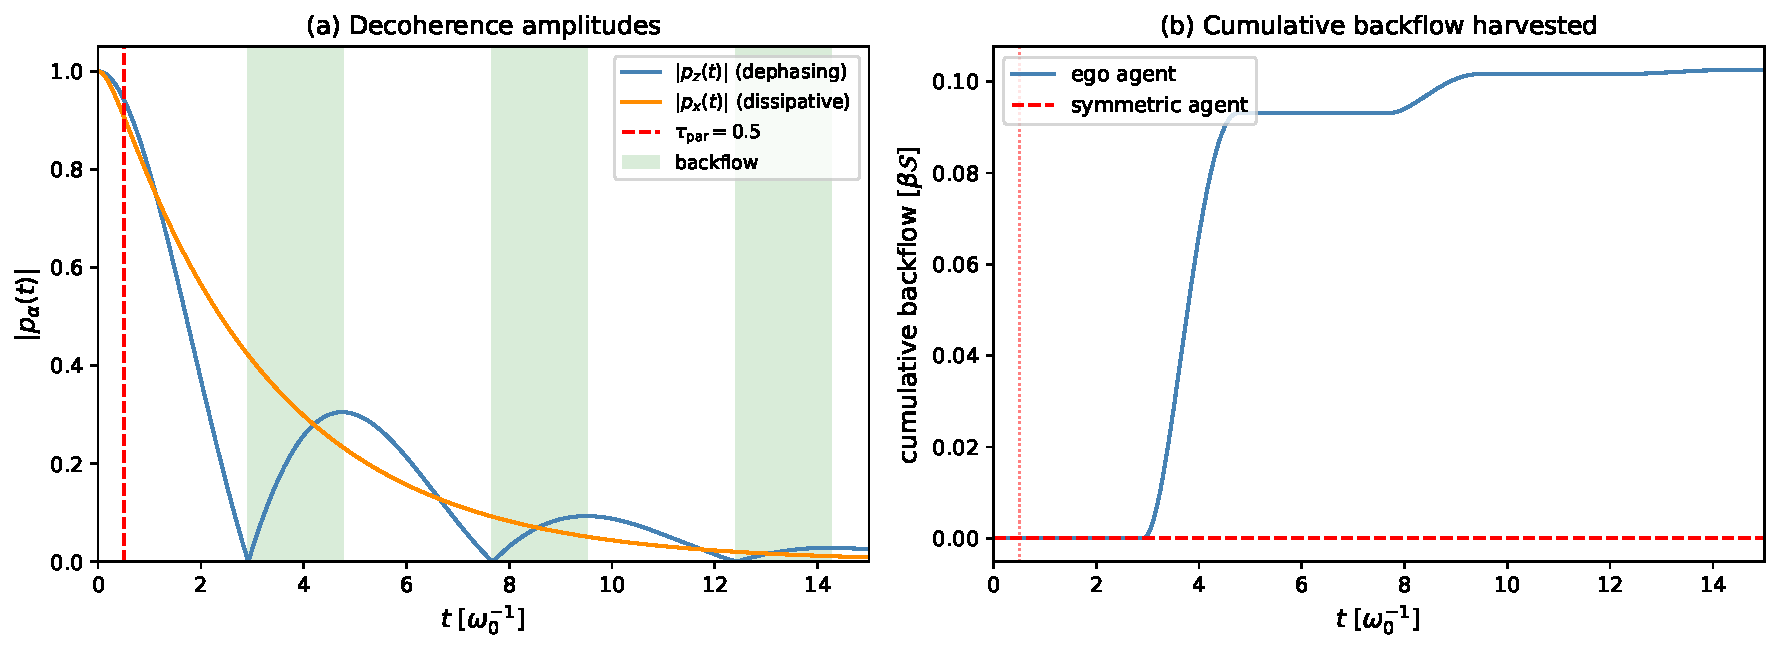
\includegraphics[width=\textwidth]{fig_ego.pdf}
\caption{%
Two-channel qubit model (Section~\ref{T-II-sec:example}) with
Lorentz--Drude spectral density.
\textbf{Parameters:}
$\omega_0 = 1$ (energy unit);
$\lambda_z = 1$, $\gamma_z = 0.5$ (dephasing, non-Markovian);
$\lambda_x = 0.3$, $\gamma_x = 5.0$ (dissipative,
$\sim$Markovian);
$\mathcal{C}_{\mathrm{budget}} = 2\,h_\mu$.
\textbf{Units:} time in $\omega_0^{-1}$.
\textbf{Regime:} low temperature ($\beta\omega_0 \gg 1$);
using the standard $T \to 0$ analytic
expression~\eqref{T-II-eq:decoherence_II}~%
\cite{BreuerPetruccione2002}.
\textbf{(a)}~Decoherence amplitudes $|p_z(t)|$ (blue,
non-Markovian, with backflow in green bands) and
$|p_x(t)|$ (orange, monotonic decay).
Red dashed: raw full-sweep depth $\tau_{\max} = 0.5$.
\textbf{(b)}~Cumulative backflow harvested.
Blue: ego agent (broken $\to \sigma_z$) exploits all three
revival intervals.
Red dashed: the stipulated raw full-sweep agent stops at
$\tau_{\max}$; all plotted backflow occurs later.
The growing gap is the \emph{ego dividend}.}
\label{T-II-fig:ego}
\end{figure}

\paragraph{Accounting check.}
The raw update load is $h_\mu D=4h_\mu$ while the budget is
$2h_\mu$, so that declared representation does not fit.  The example
then \emph{chooses} the two-component dephasing frame ($k^*=2$); for
that choice,
$R_{\mathcal{F}} = 2\,h_\mu
= \mathcal{C}_{\mathrm{budget}}$.  Saturation is an example property,
not a general consequence of monotonic distortion.

% ------------------------------------------------------------
\subsection{The Pointer-State Connection}
\label{T-II-subsec:pointer}

In this example the chosen basis coincides with an einselection
(environment-induced superselection) basis of the dephasing
model~\cite{Zurek2009}.
The coordinate optimization can select pointer-aligned components when
the declared distortion assigns them the highest survival value per
bit.  This alignment is verified only within a concrete model and is not
generic rate-distortion theorem.

\begin{remark}[Decoherence as symmetry-breaking catalyst]
\label{T-II-rem:decoherence}
The environment does not \emph{force} a specific gauge fixing.  A
pointer-aligned frame is selected only if the declared distortion and
encoder class rank it above the alternatives.  The present example
chooses that ranking; it does not derive it from bounded computation.
\end{remark}

% ============================================================
\section{The Cost of Ego}
\label{T-II-sec:cost}

Coordinate selection reduces the declared raw load but can introduce a
blind subspace. A fixed reference frame is a \emph{static}
gauge choice in a \emph{dynamic} environment.
If the environment changes, the ego becomes progressively
maladaptive.

\paragraph{Drift layer.}
Environmental change can occur at multiple levels:
parameter drift ($\lambda_\alpha(t)$, $\gamma_\alpha(t)$),
spectral-density deformation ($J(\omega, t)$), or
full process-distribution shift ($P_t(X)$).
For analytical tractability, we model drift at the
\emph{spectral-density parameter level} throughout this
section.  No monotone extension to arbitrary distribution shift is
claimed.

% ------------------------------------------------------------
\subsection{The Rigidity Trap}
\label{T-II-subsec:rigidity}

\begin{proposition}[Frame Rigidity under Drift]
\label{T-II-prop:rigidity}
Let the environment undergo slow drift: the spectral density
parameters change as
$\lambda_\alpha(t) = \lambda_\alpha^{(0)}
+ \varepsilon\,f_\alpha(t)$
for $\alpha \in \{z, x\}$, with drift rate
$\varepsilon > 0$.
Assume the supplied distortion has a locally unique $C^1$
minimizer $\mathcal{F}^*(\lambda)\in G$ and
$\lVert D_\lambda\mathcal F^*\rVert\leq K$ along the path.

If the agent's reference frame $\mathcal{F}$ is held fixed
(no recalibration), the mismatch between $\mathcal{F}$
and $\mathcal{F}^*(t)$ then obeys
\begin{equation}
\label{T-II-eq:mismatch}
\delta(t)
:= d_G\bigl(\mathcal{F},\, \mathcal{F}^*(t)\bigr)
\leq K\varepsilon \int_0^t \lVert\dot{f}(s)\rVert\,ds,
\end{equation}
where $d_G$ is the geodesic distance in the gauge group.
\end{proposition}

\begin{proof}
The chain rule and the stated sensitivity bound give
$\lVert\dot{\mathcal F}^*(t)\rVert
\leq K\varepsilon\lVert\dot f(t)\rVert$.
Integrating path length bounds the geodesic distance and yields
\eqref{T-II-eq:mismatch}.
\end{proof}

% ------------------------------------------------------------
\subsection{Stylized Drift Model}
\label{T-II-subsec:drift_model}

To quantify the loss of visibility of a fixed frame, we use the linear
drift supported by Proposition~\ref{T-II-prop:rigidity}.  No unstable
environmental dynamics or Lyapunov exponent is assumed.

\begin{definition}[Rotating optimal frame]
\label{T-II-def:drift}
Let the mismatch angle $\theta(t)$ between the agent's
fixed frame $\mathcal{F}$ and the instantaneous optimal
frame $\mathcal{F}^*(t)$ evolve as
\begin{equation}
\label{T-II-eq:theta}
\theta(t) = \theta_0+\varepsilon t,
\end{equation}
where $\theta_0 \in (0, \pi/4)$ is the initial misalignment
(so that the crossover time below is positive) and
$\varepsilon>0$ is the angular drift rate.  This is a local model up to
the first visibility crossover, not a claim about long-time motion on
the compact gauge group.

The visible and hidden survival components decompose
geometrically:
\begin{equation}
\label{T-II-eq:vis_hid_theta}
\mathcal{S}_{\mathrm{vis}}(t)
= \mathcal{S}_{\mathrm{tot}}\,\cos^2\theta(t),
\qquad
\mathcal{S}_{\mathrm{hid}}(t)
= \mathcal{S}_{\mathrm{tot}}\,\sin^2\theta(t),
\end{equation}
where $\mathcal{S}_{\mathrm{tot}}$ is the full survival
functional (invariant under frame rotation).
\end{definition}

% ------------------------------------------------------------
\subsection{The Prediction Error Divergence}
\label{T-II-subsec:divergence}

\begin{proposition}[Growth of the hidden component]
\label{T-II-prop:divergence}
Under the drift model~\eqref{T-II-eq:theta}--\eqref{T-II-eq:vis_hid_theta},
the hidden survival component grows as
\begin{equation}
\label{T-II-eq:divergence}
\bigl|\mathcal{S}_{\mathrm{hid}}(t)\bigr|
= |\mathcal{S}_{\mathrm{tot}}|\,\sin^2\!\bigl(\theta_0+
  \varepsilon t\bigr).
\end{equation}
For small angles ($\theta_0+\varepsilon t \ll 1$):
$|\mathcal{S}_{\mathrm{hid}}| \approx
|\mathcal{S}_{\mathrm{tot}}|(\theta_0+\varepsilon t)^2$.
\end{proposition}

\begin{proof}
Direct substitution of~\eqref{T-II-eq:theta}
into~\eqref{T-II-eq:vis_hid_theta}.
The small-angle expansion $\sin^2\theta\approx\theta^2$ gives the
quadratic form.
\end{proof}

% ------------------------------------------------------------
\subsection{Visibility Crossover and Conditional Gradient Reversal}
\label{T-II-subsec:delusion}

\begin{proposition}[Visibility crossover and a conditional gradient reversal]
\label{T-II-prop:delusion_model}
Under~\textup{(B1)--(B5)} with the drift
model~\eqref{T-II-eq:theta} and initial misalignment
$\theta_0 \in (0,\,\pi/4)$, an agent with a fixed
reference frame $\mathcal{F}$ reaches the visibility crossover
\begin{equation}
\label{T-II-eq:t_delusion}
t_{\mathrm{vis}}
= \frac{\pi/4-\theta_0}{\varepsilon},
\end{equation}
at which the hidden and visible magnitudes are equal.  For
$t>t_{\mathrm{vis}}$, the hidden magnitude is larger while
$\theta(t)<\pi/2$.  This geometric crossover alone implies neither
gradient anti-correlation nor failure of every in-frame detector.

There nevertheless exist specified controllers for which gradients do
reverse.  In the two-mode model
\begin{equation}
\label{T-II-eq:two_mode_losses}
\mathcal S_{\mathrm{vis}}(u)=-\tfrac12(u-1)^2,
\qquad
\mathcal S_{\mathrm{full}}(u,\theta)
=-\tfrac12\lVert u e_1-y^*(\theta)\rVert^2,
\quad
y^*(\theta)=\cos\theta\,e_1+\sin\theta\,e_2,
\end{equation}
the two scalar update directions are anti-correlated exactly when
\begin{enumerate}
\item[] $\cos\theta(t)<u<1$.
\end{enumerate}
Thus the reversal time is controller- and state-dependent; it need not
coincide with $t_{\mathrm{vis}}$.
\end{proposition}

\begin{proof}
The crossover $|\mathcal{S}_{\mathrm{hid}}|
= |\mathcal{S}_{\mathrm{vis}}|$ occurs when
$\sin^2\theta = \cos^2\theta$, i.e.,
$\theta(t_{\mathrm{vis}}) = \pi/4$.
Substituting~\eqref{T-II-eq:theta}:
$\theta_0+\varepsilon t_{\mathrm{vis}} = \pi/4$,
which gives~\eqref{T-II-eq:t_delusion}.
For~\eqref{T-II-eq:two_mode_losses},
$\partial_u\mathcal S_{\mathrm{vis}}=1-u$ and
$\partial_u\mathcal S_{\mathrm{full}}=\cos\theta-u$.
Their product is negative exactly when $u$ lies strictly between
$\cos\theta$ and $1$.  Outside that interval the two gradients agree
in sign or one vanishes.  The calculation exhibits the claimed effect
without promoting it to a universal consequence of visibility loss.
\end{proof}

\begin{remark}[Model scope]
\label{T-II-rem:linear_drift}
For $\theta_0=0$, the crossover occurs at
$t_{\mathrm{vis}} = \pi/(4\varepsilon)$.
With $\varepsilon = 0.01\,\omega_0$,
$t_{\mathrm{vis}} \approx 79\,\omega_0^{-1}$---long
enough for the agent to accumulate a false sense of
security, yet short on environmental timescales.
Neither this number nor the two-mode sign condition proves that an
agent cannot detect drift from residual statistics; Paper~III studies
one such detector.
\end{remark}

\begin{remark}[Why dithering does not help]
\label{T-II-rem:dithering}
One might ask whether the agent could escape the delusion
trap by randomly ``probing'' the background subspace
$V_{\mathrm{bg}}$---temporarily rotating its frame to
sample hidden components.
In the raw-coordinate model, a full probe competes with foreground
processing at the component-count rate in
Remark~\ref{T-II-rem:symmetry_tax}.  This does not prove dithering fails:
randomized exploration can reveal hidden directions, with a
model-dependent cost--benefit trade-off.  A deterministic in-frame
controller may lack a signal indicating when or where to probe.
As long as $|\mathcal{S}_{\mathrm{hid}}|
< |\mathcal{S}_{\mathrm{vis}}|$ (pre-delusion), the
in-frame performance metric $\mathcal{S}_{\mathrm{vis}}$
shows no anomaly.
The linear-drift visibility model below motivates monitoring residual
statistics, the subject of Paper~III, but does not rule out other
exploration policies.
\end{remark}

\begin{remark}[The ego as medicine and poison]
\label{T-II-rem:medicine_poison}
In this model, coordinate selection reduces raw load but creates a blind
subspace.  The visibility crossover below motivates Paper~III.  This is
a conditional engineering trade-off, not an irreversible logic chain.
\end{remark}

% ------------------------------------------------------------
\subsection{The Origin of Paper~III}
\label{T-II-subsec:paper3}

To respond to the visibility loss in this model, the agent may use a mechanism
to monitor the quality of its own reference frame---to
``observe its own observation.''
This requires a \emph{second-order control loop}: a
meta-controller that adjusts the gauge fixing $\sigma$ in
response to accumulated prediction errors.

The distribution of in-frame prediction residuals can itself change as
the frame becomes stale.  Paper~III studies whether a specified
likelihood model makes that change statistically identifiable.  This
paper does not prove that Fisher information is the unique detector or
that every controller must add such a loop.

This is the subject of Paper~III: the Fisher information
geometry of self-referential calibration, and the
thermodynamic cost of the loop that closes the chain
\emph{Chaos $\to$ Time $\to$ Self $\to$ Calibration}.

% ============================================================
\section{Numerical Demonstration}
\label{T-II-sec:numerical}

The preceding sections establish analytic bounds and a
worked example with a qubit in a two-channel bath.
We now compare budgeted coordinate-selection rules in a minimal
multi-dimensional system.  The observed attention concentration and
selection advantage are properties of this supplied algorithm and
environment.
Full code and parameters are provided for reproducibility.

% ------------------------------------------------------------
\subsection{Model}
\label{T-II-subsec:demo_model}

\paragraph{Environment.}
A $D$-dimensional linear prediction task with sparse
rotating support:
$y(t) = \mathbf{w}^*(t)^\top \mathbf{x}(t) + \xi(t)$,
$\mathbf{x}(t) \sim \mathcal{N}(\mathbf{0}, \mathbf{I}_D)$,
$\xi \sim \mathcal{N}(0, \sigma^2)$.
Only $m \ll D$ dimensions carry nonzero weight at any time;
the active support rotates every $\tau_{\mathrm{switch}}$
steps, modelling environmental drift.

\paragraph{Hard budget constraint.}
Per step, the agent may update only $k$ coordinates of its
weight vector (a hard processing budget), mirroring the
bounded computation assumption~(B2).

\paragraph{Agents.}
\begin{itemize}
\item \textbf{Budgeted selector}: selects the top-$k$
  dimensions by importance score---an exponential moving
  average of the signed per-coordinate gradient.  Signed
  accumulation ensures that noise dimensions (zero expected
  signal) cancel over time while signal dimensions persist,
  enabling reliable discrimination without access to the true
  support.
\item \textbf{Random-$k$ baseline}: selects $k$ dimensions
  uniformly at random each step.  This provides a
  budget-fair comparison with no persistent coordinate preference.
\end{itemize}

\noindent
The choice of \emph{signed} gradient EMA (rather than
squared-gradient magnitude) is structurally motivated:
for noise dimensions $\mathbb{E}[r\,x_i] = 0$, so the
signed accumulation cancels over time; for signal
dimensions $\mathbb{E}[r\,x_i] \neq 0$, so a consistent
directional bias persists.  The signed EMA thus acts as a
\emph{directional coherence filter} that discriminates
signal from noise without access to the true support---a
minimal model of a persistent coordinate preference.

\paragraph{Parameters.}
\begin{center}
\small
\begin{tabular}{@{}lcl@{}}
\toprule
\textbf{Quantity} & \textbf{Value} & \textbf{Role} \\
\midrule
$D$ & 64 & ambient dimension \\
$m$ & 8  & signal dimensions (sparse support) \\
$T$ & $10{,}000$ & horizon per trial \\
Seeds & 10 & independent replications \\
$\sigma$ & 0.3 & observation noise std \\
$\eta$ & 0.02 & SGD learning rate \\
$\lambda$ & 0.995 & weight decay per step \\
$k$ & 2, 4, 6, 8, 10, 12, 16, 20, 24, 32, 48, 64
  & budget grid \\
$\tau_{\mathrm{switch}}$ & $\{500, 1000, 2000\}$
  & support rotation period \\
\bottomrule
\end{tabular}
\end{center}

\paragraph{Attention entropy.}
Let $n_i$ be the number of updates coordinate $i$ receives
in a measurement window of the last $1{,}000$ steps.
The normalised update frequency
$p_i = n_i / \sum_j n_j$ defines the attention entropy:
\begin{equation}
\label{T-II-eq:H_attn}
H_{\mathrm{attn}} = -\sum_{i=1}^{D} p_i \ln p_i.
\end{equation}
Under uniform coordinate selection, $p_i = 1/D$ and
$H_{\mathrm{attn}} = \ln D$.  Under budget-constrained
selection, $H_{\mathrm{attn}}$ collapses away from $\ln D$,
measuring concentration of the update rule.  It is not by itself a
thermodynamic order parameter.

\paragraph{Oracle metric.}
Neither agent has access to $\mathbf{w}^*(t)$.
Performance is evaluated externally using the
weight-space mean-squared error
$\mathrm{MSE} = \|\hat{\mathbf{w}} - \mathbf{w}^*\|^2$,
averaged over post-burn-in steps.

% ------------------------------------------------------------
\subsection{Results}
\label{T-II-subsec:demo_results}

Figure~\ref{T-II-fig:kstar_scaling} shows the two key signatures.

\paragraph{Result 1: Attention entropy collapse
(Figure~\ref{T-II-fig:kstar_scaling}a).}
Under fixed support (no rotation), the attention entropy
$H_{\mathrm{attn}}$ exhibits a sharp collapse away from
$\ln D = \ln 64 \approx 4.16$ and increases monotonically
with $k$, consistent with a budget-induced concentration
of update mass onto signal-carrying dimensions.
For budgets near and below the signal scale ($k \leq m$),
$H_{\mathrm{attn}}$ remains $O(\ln m)$, consistent with
confinement to the signal subspace.
We use the collapse of $H_{\mathrm{attn}}$ away from
$\ln D$ as the order parameter of symmetry breaking;
a strict plateau at $\ln m$ is not expected under the
present re-selection dynamics and finite-window estimator.

\paragraph{Result 2: Selection advantage
(Figure~\ref{T-II-fig:kstar_scaling}b).}
Under rotating support, the mean-squared error gap
$\Delta\mathrm{MSE} = \mathrm{MSE}_{\mathrm{rnd}}
- \mathrm{MSE}_{\mathrm{sel}}$ is positive for
$k \lesssim 3m$ and peaks at tight budgets ($k = 2$)
where the selection advantage is strongest.
For $k \gg m$ the gap turns slightly negative
(the selector's commitment to stale dimensions costs
more than the random baseline's diversification),
before returning to zero at $k = D$.
The three $\tau_{\mathrm{switch}}$ curves are ordered:
slower drift (larger $\tau$) yields a larger peak gap,
with the ordering most visible at small $k$.

\begin{figure}[t]
\centering
\includegraphics[width=\textwidth]%
  {fig_paper2_kstar_scaling.pdf}
\caption{%
\textbf{Budgeted coordinate selection in the declared linear model.}
$D = 64$, $m = 8$, $T = 10{,}000$, 10 seeds, 95\% CI bands.
\textbf{(a)}~Attention entropy $H_{\mathrm{attn}}$ vs
budget $k$ (fixed support).  The empirical curve (blue)
collapses from $\ln D \approx 4.16$ toward an
$O(\ln m)$ floor as budget tightens.
For $k \leq m$, $H_{\mathrm{attn}}$ remains below
$\ln m \approx 2.08$ (green dashed), consistent with
confinement to the signal subspace.
\textbf{(b)}~Selection advantage
$\Delta\mathrm{MSE} = \mathrm{MSE}_{\mathrm{rnd}}
- \mathrm{MSE}_{\mathrm{sel}}$ vs budget $k$ under
rotating support.  The gap is positive for $k \lesssim 3m$
(selection helps), turns slightly negative at large $k$
(commitment cost exceeds diversification), and returns
to zero at $k = D$.  Slower drift ($\tau = 2000$)
yields a larger peak advantage.}
\label{T-II-fig:kstar_scaling}
\end{figure}

% ------------------------------------------------------------
\subsection{Scope of This Demonstration}
\label{T-II-subsec:demo_scope}

These simulations compare two supplied coordinate-selection rules in
the stated sparse linear model.  They do not establish a universal
symmetry-breaking transition or identify the capacity $k_{\max}$ with
an information-bottleneck optimum.

\medskip
This demonstration \textbf{does} show:
\begin{enumerate}
\item Under hard budget constraints, attention entropy
  collapses sharply away from $\ln D$ and remains
  $O(\ln m)$ for $k \leq m$---the agent confines its
  updates to the signal subspace.
  This measures concentration of the chosen update rule.
\item A budgeted selector that exploits importance-weighted
  selection systematically outperforms a budget-fair
  random baseline, consistent with a survival advantage
  for the parameter range shown.
\item The advantage scales with both budget tightness
  (smaller $k$) and environmental stability (larger
  $\tau_{\mathrm{switch}}$).
\end{enumerate}

\noindent
In summary, this demonstration establishes a model-specific selection
advantage and a measurable attention-concentration statistic; it does
not derive selection from the budget or claim universality across
architectures or environment classes.

\medskip
This demonstration does \textbf{not} show:
\begin{enumerate}
\item That $H_{\mathrm{attn}}$ reaches a strict plateau
  at $\ln m$ for all $k \leq m$.  Under the adaptive
  re-selection dynamics used here, the selector cycles
  within the signal subspace, producing
  $H_{\mathrm{attn}}$ values near but not locked to
  $\ln m$.  The relevant signature is the collapse
  \emph{away from} $\ln D$, not convergence to a
  specific lower bound.
\item That the specific form of the importance score
  (signed gradient EMA) is optimal.  It is one
  realisation of the selection mechanism.
\item That the results generalise to all environment
  classes.  The model uses Gaussian features, linear
  regression, and sparse rotating support.
\item That the delusion--correction cycle is addressed.
  This is the subject of Paper~III.
\item That a sharp thermodynamic phase transition occurs, or that
  $k=k_{\max}$ is the distortion-minimizing retained dimension.
\end{enumerate}

\paragraph{Reproducibility.}
\begin{sloppypar}
The complete simulation is a self-contained Python script
(\texttt{paper2\_kstar\_scaling\_demo.py}, ${\sim}\,540$
lines, requiring only NumPy and Matplotlib) with fixed
random seeds.  All figures in this section can be
reproduced by executing the script.  The following files
are included in the supplementary archive:
\begin{itemize}
\item \texttt{paper2\_kstar\_scaling\_demo.py} --- simulation script
\item \texttt{fig\_paper2\_kstar\_scaling.pdf} --- Figure~\ref{T-II-fig:kstar_scaling}
\item \texttt{kstar\_scaling\_data.csv} --- raw performance gap data
\end{itemize}
\end{sloppypar}

% ============================================================
\section{Discussion}
\label{T-II-sec:discussion}

% ------------------------------------------------------------
\subsection{Summary of Results}
\label{T-II-subsec:summary}

\begin{center}
\small
\setlength{\tabcolsep}{4pt}%
\begin{tabular}{@{}lP{6cm}c@{}}
\toprule
\textbf{Result} & \textbf{Statement} & \textbf{Sec.} \\
\midrule
Raw-channel load
  & A declared $D$-channel archive costs $D h_\mu$ per
    incremental update; this is accounting, not a lower bound
  & \ref{T-II-sec:ceiling} \\[3pt]
Compression existence
  & A minimizer exists in the supplied compact encoder class and has
    $k_{\mathrm{opt}}\leq k_{\max}$
  & \ref{T-II-subsec:RD_bound} \\[3pt]
Conditional frame selection
  & A chosen proper projection breaks the declared model symmetry when
    no invariant feasible encoder meets the target
  & \ref{T-II-subsec:SSB} \\[3pt]
Four diagnostics
  & Frame-dependent models can be audited using $\mathcal{B}_{\mathrm{select}}$,
    $\mathcal{B}_{\mathrm{frame}}$,
    $\mathcal{B}_{\mathrm{center}}$,
    $\mathcal{B}_{\mathrm{inc}}$
  & \ref{T-II-subsec:bias} \\[3pt]
Survival Decomposition
  & $\mathcal{S} = \mathcal{S}_{\mathrm{vis}} +
    \mathcal{S}_{\mathrm{hid}}$
  & \ref{T-II-subsec:effective} \\[3pt]
Uniform-channel trade-off
  & Predictive loss is approximately $1-k^*/D$ only under the
    uniform raw-channel assumption
  & \ref{T-II-subsec:tradeoff} \\[3pt]
Visibility crossover
  & Linear drift gives $t_{\mathrm{vis}}=(\pi/4-\theta_0)/\varepsilon$;
    gradient reversal requires a separate controller condition
  & \ref{T-II-subsec:delusion} \\[3pt]
Numerical demo
  & Attention concentration and model-specific selection advantage
    (Fig.~\ref{T-II-fig:kstar_scaling})
  & \ref{T-II-sec:numerical} \\
\bottomrule
\end{tabular}
\end{center}

% ------------------------------------------------------------
\subsection{Testable Predictions}
\label{T-II-subsec:predictions}

The conditional model claims can be tested without treating them as
universal laws.  First, vary $k$, $D$, and the support-switching time in
the declared sparse linear environment and compare the supplied selector
with random and alternative compressed baselines.  A sharp transition is
not predicted without a separately defined thermodynamic limit.

Second, estimate
$I(X_{\mathrm{past}};X_{\mathrm{future}})$ and
$I(\hat X_{\mathrm{past}};X_{\mathrm{future}})$ while varying $k/D$.
Linear $1-k/D$ scaling tests the uniform-allocation assumption in
Theorem~\ref{T-II-thm:tradeoff}; systematic curvature falsifies that
assumption rather than information theory.

Third, in a controlled rotating-feature task, measure both the visibility
ratio and the inner product of surrogate and oracle gradients.  The
linear model predicts the visibility crossover at
$t_{\mathrm{vis}}=(\pi/4-\theta_0)/\varepsilon$.  Proposition~\ref{T-II-prop:delusion_model}
predicts gradient reversal only for controllers entering the region
$\cos\theta(t)<u(t)<1$; coincidence of the two events is not required.

% ------------------------------------------------------------
\subsection{What This Paper Does and Does Not Show}
\label{T-II-subsec:claims}

This paper \textbf{does} show:
\begin{enumerate}
\item A declared raw $D$-channel archive has the stated component-count
  load, and a minimizer exists in the supplied compact encoder class.
\item A proper coordinate projection privileges a frame; under additional
  feasibility assumptions this can be interpreted as operational symmetry
  breaking (Remark~\ref{T-II-rem:conditional_ssb}).
\item Definition~\ref{T-II-def:bias} supplies four model diagnostics, with the
  extra controller and task assumptions needed by each made explicit.
\item Linear frame drift produces a visibility crossover, while the
  two-mode model exhibits a separate, conditional gradient reversal
  (Proposition~\ref{T-II-prop:delusion_model}).
\item A minimal computational demonstration measures attention
  concentration and a selection advantage over a budget-fair random baseline
  (Section~\ref{T-II-sec:numerical},
  Figure~\ref{T-II-fig:kstar_scaling}).
\end{enumerate}

\medskip
This paper does \textbf{not} show:
\begin{enumerate}
\item That bounded computation uniquely determines a privileged basis,
  forces symmetry breaking, or makes the chosen frame survival-optimal.
\item That symmetry breaking is necessary or sufficient for persistence.
\item That the ``ego'' implies or requires consciousness,
  subjective experience, or phenomenal awareness.
  The term is used strictly in the control-theoretic sense.
\item That this framework constitutes a theory of
  consciousness. It is a theory of computational optimality
  under thermodynamic constraints.
\item That the four diagnostics exhaust self-reference or follow from
  gauge fixing alone.
\item That the coordinate capacity is a Shannon rate--distortion bound or
  is achievable by a specific physical implementation.
\item That visibility loss forces gradient reversal or is undetectable.
  Paper~III analyzes one conditional calibration model.
\item That the framework constitutes or implies a
  philosophical or metaphysical claim about the nature
  of selfhood.
\item That this framework applies to all possible physical
  systems. It applies to systems
  satisfying the declared channel, encoder, controller, and drift
  assumptions.
\item That the Clifford algebra is the only possible
  algebraic setting. It is supplied here as a model input; Q-RAIF does
  not uniquely derive it.
\end{enumerate}

% ============================================================
% REFERENCES
% ============================================================

% ============================================================================
% Paper III --- ``The Loop''
% ============================================================================
\chapter{Fisher Information Geometry and Conditional Implementation Costs of Self-Referential Calibration}
\label{T-chap:paperIII}

\begin{center}
\textit{Paper III --- ``The Loop''}\\[0.5em]
Originally published: Zenodo, DOI: 10.5281/zenodo.18591771
\end{center}

\bigskip

\section*{Abstract}
Papers~I and~II of the T-DOME
series~\cite{Liu2026TDOME_I,Liu2026TDOME_II} supply conditional
resource and reference-frame models for persistent agents.  They do not
prove that all persistent agents require non-Markovian memory or
spontaneous Clifford gauge-symmetry breaking.  Paper~II's linear-drift
visibility crossover is likewise a declared coordinate model, not a
universal logarithmic ``Delusion Trap'' timescale.

This paper studies \textbf{self-referential calibration} under explicit
residual-likelihood, prior, drift, convexity, and hardware assumptions.
The agent uses the score statistics of a supplied prediction-residual
model to estimate frame mismatch.  The principal conditional results are:
\begin{enumerate}
\item \textbf{Gaussian Fisher Signal}
  (Proposition~\ref{T-III-prop:gaussian_fisher}):
  in the declared even Gaussian residual model, per-sample local Fisher
  information grows quadratically and accumulated information grows
  cubically.  Detection precedes the visibility crossover if and only if
  the threshold condition in Corollary~\ref{T-III-cor:detection_window} holds.
\item \textbf{Self-Referential Cram\'{e}r--Rao Bound}
  (Theorem~\ref{T-III-thm:SRCR}):
  the van Trees lower bound applies under the stated regular likelihood,
  conditional-independence, compact-support, and prior assumptions, with
  data and prior Fisher information entering separately.
\item \textbf{Conditional Implementation Cost}
  (Proposition~\ref{T-III-prop:loop_cost_impl}):
  a separable implementation with declared irreversible sensor and
  computational resets and linear-response actuation obeys
  $\dot{W}_{\mathrm{loop}}
  \geq k_BT\,\ln 2\,(R_s+R_c)
  + \mathcal{L}^2/\tau_{\mathrm{recalib}}^2$,
  a bound for that implementation rather than a universal cost of
  sensing, Fisher evaluation, or self-reference.
\end{enumerate}

The calibration loop has a local tracking bound only under geodesic
strong convexity and bounded drift (Theorem~\ref{T-III-thm:loop_stability}).
The four supplied layers in Definition~\ref{T-III-def:four_part_template}
define the running model architecture; they are not proved necessary,
sufficient, minimal, or complete for persistent agency.  ``Reflexivity''
here denotes one implementation of second-order control, with no claim of
architectural uniqueness or phenomenal consciousness.


% ============================================================
\section{Introduction}
\label{T-III-sec:intro}

% ------------------------------------------------------------
\subsection{Context: The Delusion Trap}
\label{T-III-subsec:delusion_context}

Revised Paper~II~\cite{Liu2026TDOME_II} studies a supplied
coordinate projection under a raw-channel budget.  It does not prove
that persistence forces Clifford gauge symmetry breaking.  Its drift
model uses a linearly changing mismatch
$\theta(t)=\theta_0+\varepsilon t$ and identifies the geometric
visibility crossover
\begin{equation}
\label{T-III-eq:t_del_recall}
t_{\mathrm{vis}}
=\frac{\pi/4-\theta_0}{\varepsilon}.
\end{equation}
That crossover does not by itself imply gradient reversal or
undetectability.  The present paper asks a narrower question: for a
specified residual likelihood, can score statistics detect mismatch,
and under what conditions can a natural-gradient controller track a
moving optimum?

% ------------------------------------------------------------
\subsection{Position within Papers~I--III}
\label{T-III-subsec:sequence}

This paper is the third and final of the T-DOME framework,
closing the three-paper sequence.

\begin{center}
\small
\setlength{\tabcolsep}{4pt}%
\begin{tabular}{@{}lP{3.5cm}P{4.2cm}c@{}}
\toprule
\textbf{Framework} & \textbf{Question} & \textbf{Result}
  & \textbf{Status} \\
\midrule
HAFF~\cite{Liu2026HAFF_A,Liu2026HAFF_B}
  & How does geometry emerge?
  & Conditional algebra/dictionary models
  & Revised \\[3pt]
Q-RAIF~\cite{Liu2026QRAIF_A,Liu2026QRAIF_B}
  & What algebra must an observer have?
  & Clifford representations as model inputs
  & Revised \\[3pt]
T-DOME~I~\cite{Liu2026TDOME_I}
  & What can inter-epoch correlations fund?
  & Restricted baseline; correlation accounting
  & Conditional \\[3pt]
T-DOME~II~\cite{Liu2026TDOME_II}
  & When can a model select a frame?
  & Conditional coordinate selection
  & Conditional \\[3pt]
\textbf{T-DOME~III} (this work)
  & How does self-calibration arise?
  & Fisher self-referential bound;
    thermodynamic cost of reflexivity
  & \textbf{This paper} \\
\bottomrule
\end{tabular}
\end{center}

The three T-DOME papers form a conditional modelling sequence:
\begin{enumerate}
\item \textbf{Paper~I:} Initial correlations can enter an ELV-type
  thermodynamic balance; a restricted autonomous baseline is proved.
\item \textbf{Paper~II:} A raw-coordinate archive motivates a supplied
  compression model and a linear visibility-crossover example.
\item \textbf{Paper~III (this work):} Uncorrected
  bias diverges from a changing environment.
  A self-referential calibration loop---monitoring the
  Fisher information of one's own prediction stream---resolves
  mismatch under explicit likelihood and convexity assumptions.  A
  conditional hardware model assigns reset and actuation costs.
\end{enumerate}

The links are motivation and model interfaces, not an irreversible
theorem chain.  None of the three papers proves that this architecture
is necessary for persistence.

% ------------------------------------------------------------
\subsection{The Information-Geometric Insight}
\label{T-III-subsec:insight}

The key observation that resolves the Delusion Trap is
subtle:
\emph{while the agent cannot observe $V_{\mathrm{bg}}$
directly, it can observe the statistical properties of its
own prediction residuals in $V_{\mathrm{fg}}$.}

The prediction residual
$e(t) := \mathcal{S}_{\mathrm{vis}}(t)
- \mathcal{S}_{\mathrm{vis}}^{(\mathrm{pred})}(t)$
lies in $V_{\mathrm{fg}}$ by construction.
In the declared even Gaussian model, a record cannot identify the sign
of mismatch.  Its \emph{distribution}---the probability law
$p(e\,|\,\sigma)$, parametrised by the gauge-fixing
parameter~$\sigma$---does depend on~$\sigma$, because the
projection $\Pi_{\mathcal{F}}(\sigma)$ determines which
environmental correlations are captured and which are
discarded.

When the frame $\sigma$ drifts away from the optimal
$\sigma^*$, the residual distribution shifts.
The \emph{Fisher information metric}
\begin{equation}
\label{T-III-eq:fisher_preview}
g_{ij}(\sigma)
= \mathbb{E}_\sigma\!\left[
  \frac{\partial \log p(e\,|\,\sigma)}
       {\partial \sigma^i}\,
  \frac{\partial \log p(e\,|\,\sigma)}
       {\partial \sigma^j}
\right]
\end{equation}
measures the sensitivity of this distribution to changes
in~$\sigma$.
Whether $g_{ij}$ changes with staleness is likelihood-dependent.  The
Gaussian model below provides one explicit case.

This is the mathematical realisation of the
``second-order operation'' demanded by
Paper~II, Section~7.5: the agent does not need to see the
truth (the full $Cl(V,q)$), but only the \emph{rate of
change of its own prediction error} as a function of its
frame parameters.
Fisher information is one local sensitivity measure, not the unique
possible detector.

% ------------------------------------------------------------
\subsection{Relation to Architectural Incompleteness}
\label{T-III-subsec:haff_g}

Revised HAFF Paper~G~\cite{Liu2026HAFF_G} supplies
philosophy-of-science motivation rather than a fixed-point no-go
theorem.  In that motivational sense,
the self-referential calibration loop cannot \emph{eliminate}
architectural incompleteness, but it can \emph{track}
the consequences of incompleteness in real time.
The Lyapunov function $V(\sigma)$ monitors the distance
between the agent's frame and the optimal frame without
requiring access to the ``complete'' description---it
operates entirely within the agent's own predictive
statistics.

% ------------------------------------------------------------
\subsection{Scope and Disclaimers}
\label{T-III-subsec:scope}

\begin{enumerate}
\item \emph{Reflexivity} refers throughout to
  second-order control: the ability of a system to
  monitor and adjust its own monitoring process.
  It carries \emph{no} implication of phenomenal
  consciousness, subjective experience, or qualia.
\item The self-referential calibration loop does not
  \emph{eliminate} the ego's bias; it tracks and
  compensates for drift in the bias.
  The four bias terms of Paper~II persist in the
  calibrated phase.
\item The thermodynamic cost statement is conditional on irreversible
  reset, separable hardware, and a linear-response actuation model.
\item The framework applies to systems
  satisfying~(C1)--(C5) (Section~\ref{T-III-subsec:standing_C}).
  It is not a universal theory of agency.
\end{enumerate}

\paragraph{Related work.}
The Fisher information metric on statistical manifolds was
introduced by Rao~\cite{Rao1945} and shown to be unique
by \v{C}encov~\cite{Cencov1982}.
The natural gradient and information geometry were developed
by Amari~\cite{Amari1998,AmariNagaoka2000}.
Thermodynamic length and optimal finite-time transformations
were established by
Crooks~\cite{Crooks2007} and
Sivak--Crooks~\cite{SivakCrooks2012}.
The connection between Fisher information and entropy
production was formalised by Ito~\cite{Ito2018} and
Barato--Seifert~\cite{BaratoSeifert2015}.
Second-order cybernetics originates with
Ashby~\cite{Ashby1956} and
von Foerster~\cite{vonFoerster2003}.
Adaptive control and self-tuning regulators are treated
in~\cite{AstromWittenmark1995}.
The Bayesian Cram\'{e}r--Rao bound (van Trees inequality)
is from~\cite{vanTrees1968}.

\paragraph{Summary of contributions.}
This paper separates three levels of result:
\begin{enumerate}
\item \textbf{Drift Detectability}
  (Proposition~\ref{T-III-prop:gaussian_fisher}): an explicit Gaussian
  residual likelihood has quadratic per-sample and cubic accumulated
  local Fisher signals; early detection is a threshold condition.
\item \textbf{Self-Referential Cram\'{e}r--Rao Bound}
  (Theorem~\ref{T-III-thm:SRCR}):
  drift-estimation precision is bounded by the sum of
  data Fisher information and ego rigidity.
\item \textbf{Thermodynamic Cost}
  (Proposition~\ref{T-III-prop:loop_cost_impl}): a separable implementation
  with irreversible resets and finite-time actuation obeys a conditional
  additive bound.
\end{enumerate}

\paragraph{Result-status ledger.}
The original drift-detectability theorem
\texttt{TD-III-T3.3} is retracted;
Proposition~\ref{T-III-prop:gaussian_fisher} is an FD/I model calculation and
Corollary~\ref{T-III-cor:detection_window} is conditional on a declared
threshold.  Ego rigidity \texttt{TD-III-ego} remains a supplied prior
model.  The tracking theorem is conditional on local geodesic strong
convexity.  The universal additive-cost claim
\texttt{TD-III-T6.2} is downgraded to
Proposition~\ref{T-III-prop:loop_cost_impl}, and the inherited persistence
budget is withdrawn.

% ============================================================
\section{Mathematical Preliminaries}
\label{T-III-sec:prelim}

% ------------------------------------------------------------
\subsection{Inherited Framework from Papers~I and~II}
\label{T-III-subsec:inherited}

We briefly recall the key objects; the reader is referred to
Papers~I and~II for full definitions and proofs.

\paragraph{From Paper~I~\cite{Liu2026TDOME_I}.}
\begin{itemize}
\item \textbf{Survival functional.}
  $\mathcal{S}[\Lambda,\tau]
  := \Delta F - W[0,\tau]$~(Paper~I,
  Eq.~(9)).
\item \textbf{Restricted autonomous baseline.}
  $\mathcal{S}[\Lambda^{\mathrm{D}},\tau]\leq0$ for a fixed-Hamiltonian,
  no-control Davies semigroup under its stated initial conditions.  It
  is not a ceiling for all Markovian agents.
\item \textbf{Memory kernel.}
  $\mathcal{K}(t,s)$: the non-Markovian superoperator
  encoding system--environment correlations.
\item \textbf{Entropy rate.}
  $h_\mu := \lim_{T\to\infty}T^{-1}H(X_{0:T})$ (bits per
  unit time per algebraic component).
\item \textbf{Predictive information.}
  $I_{\mathrm{pred}}
  := I(\overleftarrow{X};\,\overrightarrow{X})$.
\end{itemize}

\paragraph{From Paper~II~\cite{Liu2026TDOME_II}.}
\begin{itemize}
\item \textbf{Internal algebra.}
  $\mathcal{O}_{\mathrm{int}} = Cl(V,q)$, $D = \dim Cl(V,q) = 2^n$,
  gauge group $G = \mathrm{Aut}(Cl(V,q))$.
\item \textbf{Gauge bundle.}
  $\pi: P \to M$, structure group $G$; a section
  $\sigma: M \to P$ is a reference frame.
\item \textbf{Ego.}
  $\mathfrak{E} := (\mathcal{F}^*,\,V_{\mathrm{fg}}^*)$
  denotes a chosen optimizer in a supplied encoder class, with
  $k^*=k_{\mathrm{opt}}\leq k_{\max}$.  The budget capacity is not a
  universal optimizer formula.
\item \textbf{Projected kernel.}
  $\mathcal{K}_{\mathcal{F}}(t,s)
  = \Pi_{\mathcal{F}}\,\mathcal{K}(t,s)\,
  \Pi_{\mathcal{F}}$.
\item \textbf{Survival decomposition.}
  $\mathcal{S} = \mathcal{S}_{\mathrm{vis}}(\mathcal{F})
  + \mathcal{S}_{\mathrm{hid}}(\mathcal{F})$.
\item \textbf{Four bias terms.}
  $\mathcal{B}_{\mathrm{select}}$,
  $\mathcal{B}_{\mathrm{frame}}$,
  $\mathcal{B}_{\mathrm{center}}$,
  $\mathcal{B}_{\mathrm{inc}}$
  (revised Paper~II, four-diagnostics definition).  These are model
  diagnostics, not generic consequences of gauge fixing.
\item \textbf{Visibility crossover.}
  $t_{\mathrm{vis}}=(\pi/4-\theta_0)/\varepsilon$ in the supplied
  linear drift geometry.  Gradient reversal requires an additional
  controller condition.
\item \textbf{Information objects.}
  Mutual information is evaluated on explicitly induced record
  processes; algebra symbols are not themselves random variables.
\end{itemize}

% ------------------------------------------------------------
\subsection{Fisher Information Metric}
\label{T-III-subsec:fisher}

\begin{definition}[Fisher information matrix]
\label{T-III-def:fisher}
Let $\{p(x\,|\,\theta) : \theta \in \Theta
\subset \mathbb{R}^d\}$ be a parametric family of
probability densities satisfying standard regularity
conditions (interchange of differentiation and integration).
The \emph{Fisher information matrix} is
\begin{equation}
\label{T-III-eq:fisher_def}
g_{ij}(\theta)
:= \mathbb{E}_\theta\!\left[
  \frac{\partial \log p(x\,|\,\theta)}
       {\partial \theta^i}\,
  \frac{\partial \log p(x\,|\,\theta)}
       {\partial \theta^j}
\right]
= -\mathbb{E}_\theta\!\left[
  \frac{\partial^2 \log p(x\,|\,\theta)}
       {\partial \theta^i\,\partial \theta^j}
\right].
\end{equation}
The pair $(\Theta,\,g)$ is a Riemannian manifold called the
\emph{statistical manifold}.
\end{definition}

\begin{remark}[Uniqueness]
\label{T-III-rem:cencov}
By \v{C}encov's theorem~\cite{Cencov1982}, the Fisher--Rao
metric $g^{\mathrm{FR}}$ is, up to a positive scalar
multiple, the unique Riemannian metric on the space of
probability distributions that is invariant under all
Markov morphisms (sufficient-statistic embeddings).
Within the hypotheses and category used by \v{C}encov's theorem, this
makes the Fisher metric a canonical local distinguishability metric.
It does not make a Fisher-based detector physically mandatory, nor does
it choose a likelihood or control objective for the agent.
\end{remark}

\begin{proposition}[Cram\'{e}r--Rao bound]
\label{T-III-prop:CR}
For any unbiased estimator $\hat{\theta}$ of $\theta$ based
on $n$ independent observations:
\begin{equation}
\label{T-III-eq:CR}
\mathrm{Cov}(\hat{\theta})
\;\succeq\; \frac{1}{n}\,\bigl[g(\theta)\bigr]^{-1}
\end{equation}
in the L\"{o}wner order.
The scalar case reads
$\mathrm{Var}(\hat{\theta})
\geq 1/\bigl(n\,g(\theta)\bigr)$.
\end{proposition}

\begin{remark}[Effective independence]
\label{T-III-rem:effective_independence}
Throughout this paper, references to ``independent
observations'' in the context of continuous-time residual
streams should be read as \emph{effective independence}
after thinning by the environmental decorrelation
time~$\tau_E$, yielding an effective sample size
$n_{\mathrm{eff}} \approx T/\tau_E$.
In particular, the sample count $n$ in~\eqref{T-III-eq:CR}
becomes $n_{\mathrm{eff}}$ in the self-referential
setting of Section~\ref{T-III-subsec:SRCR}.
\end{remark}

\begin{remark}[Fisher metric and KL divergence]
\label{T-III-rem:fisher_KL}
The Fisher metric arises as the Hessian of the
Kullback--Leibler divergence~\cite{CoverThomas2006}:
\begin{equation}
\label{T-III-eq:fisher_KL}
D_{\mathrm{KL}}\bigl(p_\theta \,\|\, p_{\theta+d\theta}\bigr)
= \tfrac{1}{2}\,g_{ij}(\theta)\,d\theta^i\,d\theta^j
  + O\!\left(|d\theta|^3\right).
\end{equation}
This identifies the Fisher metric as the infinitesimal
measure of statistical distinguishability.
\end{remark}

% ------------------------------------------------------------
\subsection{Information Geometry}
\label{T-III-subsec:info_geom}

Following Amari~\cite{Amari1985,AmariNagaoka2000}, the
statistical manifold $(\Theta,\,g)$ carries additional
geometric structure beyond the Riemannian metric.

\paragraph{$\alpha$-connections.}
For each $\alpha \in [-1,\,1]$, Amari defines an affine
connection $\nabla^{(\alpha)}$ on $\Theta$.
The cases $\alpha = 1$ (exponential connection,
$\nabla^{(e)}$) and $\alpha = -1$ (mixture connection,
$\nabla^{(m)}$) are \emph{dual} with respect to $g$:
$\partial_k\,g(X,Y)
= g(\nabla_k^{(e)}X,\,Y)
+ g(X,\,\nabla_k^{(m)}Y)$.
For exponential families, $\nabla^{(e)}$ is flat in natural
parameters and $\nabla^{(m)}$ is flat in expectation
parameters---the \emph{dually flat structure}.
The case $\alpha = 0$ recovers the Levi-Civita connection of
the Fisher metric.

\paragraph{Natural gradient.}
Standard gradient descent in parameter space ignores the
curvature of the statistical manifold.
The \emph{natural gradient}~\cite{Amari1998}
\begin{equation}
\label{T-III-eq:natural_gradient}
\dot{\theta}
= -\eta\,g^{-1}(\theta)\,\nabla_\theta L(\theta),
\end{equation}
where $\eta > 0$ is the learning rate and $L(\theta)$ is a
loss function, provides the steepest descent direction in the
Fisher metric.
It is reparametrisation-invariant.  Statistical efficiency requires
additional estimator and asymptotic assumptions and is not implied by
the update formula alone.

\paragraph{Pythagorean theorem.}
In a dually flat space, the KL divergence satisfies
a generalised Pythagorean relation:
$D_{\mathrm{KL}}(p\,\|\,r)
= D_{\mathrm{KL}}(p\,\|\,q)
+ D_{\mathrm{KL}}(q\,\|\,r)$
when $q$ is the $m$-projection of $p$ onto a
submanifold containing $r$.
This decomposition will be applied to separate the
foreground-recoverable and background-irrecoverable
components of drift.

% ------------------------------------------------------------
\subsection{Thermodynamic Length}
\label{T-III-subsec:thermo_length}

\begin{definition}[Thermodynamic length]
\label{T-III-def:thermo_length}
Let $\lambda(t)$ for $t \in [0,\tau]$ be a path through
control parameter space, and let $\zeta_{ij}(\lambda)$ be the
\emph{friction tensor} (the time-integrated equilibrium
force--force correlation function at~$\lambda$).
The \emph{thermodynamic length} of the
path~\cite{Crooks2007} is
\begin{equation}
\label{T-III-eq:thermo_length}
\mathcal{L}
:= \int_0^\tau
\sqrt{\zeta_{ij}(\lambda)\,
  \dot{\lambda}^i\,\dot{\lambda}^j}\;dt.
\end{equation}
\end{definition}

\begin{proposition}[Sivak--Crooks bound]
\label{T-III-prop:sivak_crooks}
The excess (dissipated) work during a finite-time
transformation of duration $\tau$ satisfies~\cite{SivakCrooks2012}
\begin{equation}
\label{T-III-eq:sivak_crooks}
W_{\mathrm{ex}} \;\geq\; \frac{\mathcal{L}^2}{\tau}.
\end{equation}
The minimum is achieved by the geodesic of the friction
tensor $\zeta$.
In the linear-response regime, the friction tensor is
related to the Fisher metric of the equilibrium distribution
at $\lambda$ by
$\zeta_{ij}(\lambda)
\sim \tau_{\mathrm{relax}}\,g_{ij}^{\mathrm{Fisher}}(\lambda)$,
where $\tau_{\mathrm{relax}}$ is the relaxation time.
\end{proposition}

% ------------------------------------------------------------
\subsection{Second-Order Cybernetics}
\label{T-III-subsec:cybernetics}

Von Foerster~\cite{vonFoerster2003} distinguished two levels
of control:
\begin{itemize}
\item \textbf{First-order cybernetics}: feedback control of
  observed systems.
  The controller adjusts its actions based on the output of
  a sensor.
  Paper~II's ego is a first-order structure: it processes
  environmental data within a fixed frame.
\item \textbf{Second-order cybernetics}: feedback control of
  the \emph{observing} system itself.
  The controller adjusts the \emph{sensor}---or equivalently,
  the reference frame within which the sensor operates.
  This is what Paper~III provides.
\end{itemize}

Ashby's Law of Requisite Variety~\cite{Ashby1956} provides a
lower bound on the complexity of the meta-controller:
\begin{equation}
\label{T-III-eq:requisite_variety}
\dim\!\left(\text{meta-controller state space}\right)
\;\geq\; \dim\!\left(\text{environmental drift subspace}\right).
\end{equation}
The meta-observer must have at least as many adjustable
parameters as there are independent modes of environmental
drift.

In adaptive control
theory~\cite{AstromWittenmark1995}, the analogous result is
the \emph{persistent excitation} condition: parameter
estimates converge if and only if the input signal is
``rich enough'' to excite all modes of the system.
In our framework, persistent excitation corresponds to
$h_\mu > 0$---the environment must continue to generate
novelty for the self-calibration loop to function.

\begin{remark}[Operational content]
\label{T-III-rem:cybernetics_operational}
The second-order cybernetic structure in this paper is
\emph{not} a philosophical metaphor.
It has concrete operational content: the natural gradient
update~\eqref{T-III-eq:natural_gradient} is a specific algorithm
that takes as input the Fisher information of the residual
stream and produces as output an update to the frame
parameter~$\sigma$.
An implementation must supply a differentiable residual likelihood,
evaluate or approximate its score, and realize the update law.  Merely
accumulating an unlabelled residual second moment is not generally a
Fisher computation.
\end{remark}

% ------------------------------------------------------------
\subsection{Standing Assumptions}
\label{T-III-subsec:standing_C}

\begin{definition}[Standing Assumptions]
\label{T-III-def:assumptions_C}
Throughout this paper, the following conditions are assumed:
\begin{enumerate}
\item[\textup{(C1)}] \textbf{Supplied representation model.}
  A finite-dimensional agent model, a foreground projection, and a
  control algebra are specified.  A Clifford representation and any
  external map $\phi$ are model inputs, not conclusions inherited from
  revised Q-RAIF or T-DOME II.
\item[\textup{(C2)}] \textbf{Environmental drift.}
  The instantaneous optimal frame
  $\mathcal{F}^*(t)$ rotates continuously in~$G$ at
  bounded speed.  In the scalar worked model the mismatch is
  $\theta(t)=\theta_0+\varepsilon t$ up to the first visibility
  crossover, as in revised Paper~II.
\item[\textup{(C3)}] \textbf{Finite meta-observer budget.}
  The self-calibration loop has a computational budget
  $\mathcal{C}_{\mathrm{meta}} < \infty$ (bits per unit
  time), distinct from the ego's processing budget
  $\mathcal{C}_{\mathrm{budget}}$.
\item[\textup{(C4)}] \textbf{Regularity.}
  The agent's predictive family
  $\{p(e\,|\,\sigma)
  : \sigma \in G/H\}$ satisfies standard Fisher
  information regularity: finite Fisher matrix and interchange of
  differentiation and integration.  Any scalar sensitivity or uniform
  lower bound used later must be assumed separately.
\item[\textup{(C5)}] \textbf{Persistent excitation.}
  The time-averaged Fisher matrix obeys the explicit lower bound in
  Definition~\ref{T-III-def:PE_constant}.  A positive entropy rate alone is
  not sufficient for this condition.
\end{enumerate}
\end{definition}

% ============================================================
\section{The Drift Detection Problem}
\label{T-III-sec:detection}

% ------------------------------------------------------------
\subsection{Identifiability in an Even Residual Model}
\label{T-III-subsec:first_order}

\begin{proposition}[Sign non-identifiability in an even residual model]
\label{T-III-prop:first_order_nonidentifiability}
Suppose the scalar residual model is
$e\mid\theta\sim\mathcal N(a\theta^2,\sigma_e^2)$ with
$a\neq0$ and $\sigma_e>0$.  Then
$p(e\mid\theta)=p(e\mid-\theta)$ for every sample and every
record length.  Residual data alone therefore cannot identify the sign
of the frame mismatch without an orientation-breaking input.
\end{proposition}

\begin{proof}
The likelihood depends on $\theta$ only through $\theta^2$; hence the
joint likelihood of any record is invariant under
$\theta\mapsto-\theta$.  No statistic of that record can distinguish
the two parameter values.
\end{proof}

This proposition is a property of the declared even likelihood.  It
does not prove that every instantaneous or ``first-order'' controller
fails: directional probes, asymmetric residual models, and exogenous
orientation data can remove the ambiguity.

% ------------------------------------------------------------
\subsection{The Agent's Statistical Manifold}
\label{T-III-subsec:stat_manifold}

The agent's prediction-residual stream
$\{e(t)\}_{t \geq 0}$ defines a stochastic process whose
distribution depends on the gauge-fixing
parameter~$\sigma$.
We model this dependence as a parametric family.

\begin{definition}[Predictive family]
\label{T-III-def:predictive_family}
The \emph{predictive family} of the agent is the set
\begin{equation}
\label{T-III-eq:predictive_family}
\mathcal{P}
:= \bigl\{p(e\,|\,\sigma)
  : \sigma \in \mathcal{M}_G\bigr\},
\end{equation}
where $\mathcal{M}_G := G/H$ is the space of gauge-fixing
orbits ($H$ is the stabiliser of the foreground subspace),
$e$ denotes the prediction-residual time series over a
window of length~$T$, and $p(e\,|\,\sigma)$ is the
likelihood of the observed residuals given the gauge
parameter~$\sigma$.
\end{definition}

The key insight is that $p(e\,|\,\sigma)$ depends
on~$\sigma$ even though $e(t) \in V_{\mathrm{fg}}$,
because the projection $\Pi_{\mathcal{F}}(\sigma)$
determines which environmental correlations are captured.
When $\sigma$ drifts from the optimal $\sigma^*$:
\begin{itemize}
\item The variance of the residuals increases (the
  discarded background components contribute unmodelled
  noise).
\item The temporal correlations of the residuals change
  (the projected kernel $\mathcal{K}_{\mathcal{F}}$ no
  longer captures the dominant environmental modes).
\item Higher-order statistics (kurtosis, spectral shape)
  shift systematically.
\end{itemize}
These distributional changes are invisible to the
raw error $e(t)$ but detectable by the Fisher metric
of $\mathcal{P}$.

% ------------------------------------------------------------
\subsection{Self-Referential Fisher Information}
\label{T-III-subsec:self_ref_fisher}

\begin{definition}[Self-referential Fisher information]
\label{T-III-def:self_ref_fisher}
For one residual with likelihood $p(e\mid\sigma)$, define the
\emph{per-sample Fisher information}
\begin{equation}
\label{T-III-eq:self_ref_fisher}
\mathcal I_1(\sigma)
:=\mathbb E_\sigma\!\left[
  (\partial_\sigma\log p(e\mid\sigma))^2\right].
\end{equation}
For conditionally independent residuals observed at times $t_m$, the
\emph{accumulated local information} is
$J_T:=\sum_{t_m\leq T}\mathcal I_1(\sigma(t_m))$.
The Fisher metric $g$, the local quadratic form
$g_{ij}\delta\sigma^i\delta\sigma^j$, and $J_T$ are distinct
objects.  Fisher information is measured in inverse-squared parameter
units, not bits.
\end{definition}

\begin{remark}[What the agent ``measures'']
\label{T-III-rem:what_measured}
Computing $\mathcal I_1(\sigma)$ does not require access
to $V_{\mathrm{bg}}$ or to the ``true'' environment.
It requires only: (i)~the agent's own prediction residuals
$\{e(t)\}$ (which lie in $V_{\mathrm{fg}}$), and
(ii)~the ability to evaluate the score function
$\partial_\sigma \log p(e\,|\,\sigma)$---the sensitivity of
its own predictive model to frame perturbations.
This is a computation entirely within the agent's internal
algebra, using only quantities already available from the
ego's processing pipeline.
\end{remark}

\begin{proposition}[Fisher signal in a Gaussian residual model]
\label{T-III-prop:gaussian_fisher}
Let residuals sampled at rate $r$ be conditionally independent with
\begin{equation}
\label{T-III-eq:gaussian_residual}
e_m\mid\theta_m\sim\mathcal N(a\theta_m^2,\sigma_e^2),
\qquad \theta(t)=\theta_0+\varepsilon t,
\end{equation}
where $a\neq0$, $\sigma_e>0$, and $\varepsilon>0$.  The per-sample
Fisher information with respect to the current mismatch is
\begin{equation}
\label{T-III-eq:detectability}
\mathcal I_1(\theta)=\frac{4a^2\theta^2}{\sigma_e^2}.
\end{equation}
Consequently the expected accumulated local information over a window
of length $T$ is
\begin{equation}
\label{T-III-eq:accumulated_fisher}
J_T\simeq\frac{4a^2r}{3\sigma_e^2\varepsilon}
\left[(\theta_0+\varepsilon T)^3-\theta_0^3\right].
\end{equation}
For a freshly calibrated frame ($\theta_0=0$), the per-sample signal is
quadratic in time and $J_T=4a^2r\varepsilon^2T^3/(3\sigma_e^2)$.
\end{proposition}

\begin{proof}
For a normal family with fixed variance and mean
$\mu(\theta)=a\theta^2$, the score is
$(e-\mu)\mu'(\theta)/\sigma_e^2$.  Taking its squared
expectation gives $(\mu')^2/\sigma_e^2$, which is
\eqref{T-III-eq:detectability}.  Summing over samples and using the sampling
rate gives
$J_T\simeq r\int_0^T\mathcal I_1(\theta_0+\varepsilon t)dt$,
which evaluates to~\eqref{T-III-eq:accumulated_fisher}.
\end{proof}

\begin{remark}[Scope of the sensitivity claim]
\label{T-III-rem:fisher_sensitivity_scope}
Full-rank Fisher information for $\sigma$ does not imply that a scalar
mismatch map $\theta(\sigma)$ has a Jacobian bounded away from zero.
Proposition~\ref{T-III-prop:gaussian_fisher} therefore works directly in the
identified scalar mismatch coordinate.  A multi-parameter extension
must supply or derive the relevant sensitivity map.
\end{remark}

\begin{corollary}[Conditional detection before visibility crossover]
\label{T-III-cor:detection_window}
In the Gaussian residual model, let $J_{\min}>0$ be a declared
detection threshold.  For a freshly calibrated frame,
\begin{equation}
\label{T-III-eq:detection_window}
T_{\mathrm{det}}
=\left(\frac{3\sigma_e^2J_{\min}}
  {4a^2r\varepsilon^2}\right)^{1/3}.
\end{equation}
Detection precedes Paper~II's visibility crossover if and only if
$T_{\mathrm{det}}<t_{\mathrm{vis}}$, where for the same linear drift
$t_{\mathrm{vis}}=(\pi/4-\theta_0)/\varepsilon$.  Equivalently, for
general $\theta_0$ the condition is
$J_{t_{\mathrm{vis}}}>J_{\min}$.  No unconditional ordering follows
from regularity alone.
\end{corollary}

\begin{proof}
Set the fresh-calibration expression for $J_T$ in
Proposition~\ref{T-III-prop:gaussian_fisher} equal to $J_{\min}$ and solve
for $T$.  Comparing that value with the independently defined
visibility time gives the stated condition.
\end{proof}

% ============================================================
\section{The Self-Referential Bound}
\label{T-III-sec:SRCR}

% ------------------------------------------------------------
\subsection{The Bayesian Framework}
\label{T-III-subsec:bayesian}

The agent's ego structure (Paper~II) provides a
\emph{prior belief} about the correct gauge parameter:
the current frame $\sigma_0$ is the ego's
``preferred'' value.
We encode this as a prior distribution
$\pi_{\mathrm{ego}}(\sigma)$, concentrated around
$\sigma_0$.

\begin{definition}[Ego rigidity]
\label{T-III-def:ego_rigidity}
The \emph{ego rigidity} is the prior Fisher information
\begin{equation}
\label{T-III-eq:ego_rigidity}
\mathcal{I}_{\mathrm{ego}}
:= \int_{\mathcal{M}_G}
\left(\frac{\partial \log \pi_{\mathrm{ego}}(\sigma)}
  {\partial \sigma}\right)^{\!2}
\pi_{\mathrm{ego}}(\sigma)\,d\sigma.
\end{equation}
High $\mathcal{I}_{\mathrm{ego}}$ corresponds to a
sharply peaked prior (rigid ego); low
$\mathcal{I}_{\mathrm{ego}}$ to a diffuse prior (flexible
ego).
This prior and its Fisher information are supplied model data.  The
diagnostics of Paper~II do not determine a prior without an additional
statistical construction.
\end{definition}

% ------------------------------------------------------------
\subsection{The Self-Referential Cram\'{e}r--Rao Bound}
\label{T-III-subsec:SRCR}

\begin{theorem}[Self-Referential Cram\'{e}r--Rao Bound]
\label{T-III-thm:SRCR}
Let the scalar drift parameter $\delta\sigma$ lie in a compact interval
$[a,b]$.  Assume that the residual likelihood is regular, that the
effective samples are conditionally independent, and that the prior
$\pi_{\mathrm{ego}}$ is $C^1$, has finite prior Fisher information,
and vanishes at $a$ and $b$.  Let $\delta\hat\sigma$ be any estimator
based only on a residual record of duration~$T$.
Define the \emph{effective sample size}
$n_{\mathrm{eff}} := T/\tau_E$, where $\tau_E$ is the
decorrelation time of the residual process~$\{e(t)\}$
(the time beyond which consecutive residuals carry
approximately independent information about~$\sigma$).
If the effective samples share per-sample information
$\mathcal I_1(\delta\sigma)$, the van Trees
inequality~\cite{vanTrees1968} gives
\begin{equation}
\label{T-III-eq:SRCR}
\mathbb{E}\!\left[
  \bigl|\delta\hat{\sigma} - \delta\sigma\bigr|^2
\right]
\;\geq\; \frac{1}{
  n_{\mathrm{eff}}\,\mathbb E_{\pi}[\mathcal I_1(\delta\sigma)]
  + \mathcal{I}_{\mathrm{ego}}}.
\end{equation}
\end{theorem}

\begin{proof}
This is a direct application of the van Trees
(Bayesian Cram\'{e}r--Rao)
inequality~\cite{vanTrees1968}.
The total information about the drift parameter $\delta\sigma$
consists of two contributions:
\begin{itemize}
\item $n_{\mathrm{eff}}\,\mathbb E_\pi[\mathcal I_1]$: the data
  Fisher information.  In continuous time, the residual
  process is correlated with decorrelation time $\tau_E$
  set by the bath memory kernel.
  Over a window of duration~$T$, the process yields
  $n_{\mathrm{eff}} \approx T/\tau_E$ effectively
  independent samples, each carrying Fisher information
  about $\delta\sigma$.
\item $\mathcal{I}_{\mathrm{ego}}$: the prior Fisher
  information from the ego's preference for $\sigma_0$
  (Definition~\ref{T-III-def:ego_rigidity}).
\end{itemize}
The boundary and regularity assumptions remove the
integration-by-parts boundary term in the standard van Trees proof.
Fisher information is not measured in bits; the denominator has
inverse-squared parameter units.
\end{proof}

\begin{remark}[The ego as help and hindrance]
\label{T-III-rem:ego_dual}
The ego rigidity $\mathcal{I}_{\mathrm{ego}}$ acts as
both help and hindrance:
\begin{itemize}
\item \textbf{Help}: when the ego is well-aligned
  ($\sigma_0 \approx \sigma^*$), the prior tightens the
  bound, reducing estimation variance.
\item \textbf{Hindrance}: when the ego is misaligned
  ($|\sigma_0 - \sigma^*|$ large), the prior pulls the
  estimate toward the wrong value, creating a
  \emph{confirmation bias} that resists recalibration.
\end{itemize}
For a conjugate scalar Gaussian location model only, the posterior mean
has the precision-weighted form below, where
$\bar{\mathcal I}_1$ is its constant per-sample data precision:
\begin{equation}
\label{T-III-eq:optimal_estimator}
\hat{\sigma}_{\mathrm{opt}}
= \frac{n_{\mathrm{eff}}\,\bar{\mathcal I}_1\,\hat{\sigma}_{\mathrm{MLE}}
  + \mathcal{I}_{\mathrm{ego}}\,\sigma_0}
  {n_{\mathrm{eff}}\,\bar{\mathcal I}_1 + \mathcal{I}_{\mathrm{ego}}},
\end{equation}
a weighted average of the maximum-likelihood estimate
$\hat{\sigma}_{\mathrm{MLE}}$ and the ego's prior belief
$\sigma_0$, with weights proportional to their respective
Fisher informations.
This formula is not implied by van Trees for a general likelihood or
prior.  In the conjugate Gaussian case, as
$n_{\mathrm{eff}}\,\bar{\mathcal I}_1 \gg \mathcal{I}_{\mathrm{ego}}$
(enough data to overwhelm the ego), the estimator converges
to the MLE.
\end{remark}

% ------------------------------------------------------------
\subsection{The Rigidity-Sensitivity Trade-off}
\label{T-III-subsec:rigidity}

\begin{proposition}[Optimal ego rigidity]
\label{T-III-prop:optimal_rigidity}
Let the total expected loss be
$\mathcal{L}_{\mathrm{total}}
(\mathcal{I}_{\mathrm{ego}})
= \mathcal{L}_{\mathrm{estimation}}
+ \lambda\,\mathcal{L}_{\mathrm{calibration}}$,
where $\mathcal{L}_{\mathrm{estimation}}$ is the
mean-squared drift-estimation error
(bounded by~\eqref{T-III-eq:SRCR}) and
$\mathcal{L}_{\mathrm{calibration}}$ is the cost of
adjusting the frame (proportional to the frame rotation
distance, hence larger when the ego is rigid and must be
overcome).
If the admissible rigidity interval is nonempty and compact and the two
supplied loss terms are lower semicontinuous, an optimal rigidity
$\mathcal{I}_{\mathrm{ego}}^*$ exists.  Uniqueness or an interior
optimum additionally requires a model-specific strict-convexity or
monotonicity condition.

\emph{Too rigid}
($\mathcal{I}_{\mathrm{ego}} \gg n_{\mathrm{eff}}\,\bar{\mathcal I}_1$):
the ego overwhelms the data; the agent is blind to drift.
\emph{Too soft}
($\mathcal{I}_{\mathrm{ego}} \ll n_{\mathrm{eff}}\,\bar{\mathcal I}_1$):
the agent overreacts to noise; calibration cost is high.
The optimum balances sensitivity against stability.
\end{proposition}

\begin{proof}
A lower-semicontinuous real function attains its minimum on a nonempty
compact set.  The existence conclusion uses only that fact; the
qualitative ``too rigid/too soft'' interpretation is not a convexity
proof.
\end{proof}

% ============================================================
\section{The Calibration Loop}
\label{T-III-sec:loop}

% ------------------------------------------------------------
\subsection{The Natural Gradient Update Law}
\label{T-III-subsec:update_law}

The meta-observer updates the gauge parameter $\sigma$
following the natural gradient on the statistical
manifold~$(\mathcal{M}_G,\,g)$:
\begin{equation}
\label{T-III-eq:update_law}
\dot{\sigma}
= -\eta\,g^{-1}(\sigma)\,
  \nabla_\sigma L_{\mathrm{frame}}(\sigma),
\end{equation}
where $\eta > 0$ is the adaptation rate and the
\emph{frame loss} is
\begin{equation}
\label{T-III-eq:frame_loss}
L_{\mathrm{frame}}(\sigma)
:= \mathbb{E}_\sigma\!\left[
  -\mathcal{S}_{\mathrm{vis}}(\sigma)\right].
\end{equation}
The frame loss is minimised at the optimal gauge
$\sigma^*$ that maximises visible survival.
The Fisher metric enters through the inverse $g^{-1}$
in the natural gradient, not as a penalty term:
it defines the \emph{geometry} of the update, ensuring
reparametrisation invariance.

\begin{remark}[Reparametrisation invariance]
\label{T-III-rem:reparam}
The natural gradient~\eqref{T-III-eq:update_law} is invariant
under reparametrisation of the gauge manifold
$\mathcal{M}_G$: the update direction does not depend on the
choice of coordinates for $\sigma$.
This is essential because the gauge manifold inherits its
geometry from the Clifford algebra, and no canonical
coordinate system is preferred.
\end{remark}

% ------------------------------------------------------------
\subsection{Lyapunov Stability of the Loop}
\label{T-III-subsec:lyapunov}

\paragraph{Drift velocity.}
Let $\sigma^*(t)$ denote the instantaneous optimal gauge
parameter, defined as a minimiser of $L_{\mathrm{frame}}$
at time~$t$ in Eq.~\eqref{T-III-eq:frame_loss}.
Define the \emph{drift velocity}
$\dot{\sigma}^* := d\sigma^*/dt$, measured with respect to
the Fisher metric~$g$; its norm
$\|\dot{\sigma}^*\|_g
:= \sqrt{g_{ij}\,\dot{\sigma}^{*i}\,\dot{\sigma}^{*j}}$
is the instantaneous rate at which the environment's
optimal frame rotates on the gauge manifold.

\begin{definition}[Lyapunov monitoring function]
\label{T-III-def:lyapunov}
The \emph{Lyapunov monitoring function} is the squared
geodesic distance on the statistical manifold from the
current frame to the instantaneous optimal frame:
\begin{equation}
\label{T-III-eq:lyapunov}
V(\sigma)
:= d_{\mathrm{geo}}\!\left(\sigma,\,\sigma^*(t)\right)^2,
\end{equation}
where $d_{\mathrm{geo}}$ is the geodesic distance in the
Fisher metric~$g$.
\end{definition}

\begin{theorem}[Loop Tracking Bound]
\label{T-III-thm:loop_stability}
Assume the natural-gradient trajectory remains in a geodesically convex
normal neighbourhood of $\sigma^*(t)$ and that the frame loss is
geodesically $m_L$-strongly convex there, with
$\operatorname{Hess}L_{\mathrm{frame}}\succeq m_L g$ for some
$m_L>0$.  Then the update~\eqref{T-III-eq:update_law} satisfies
\begin{equation}
\label{T-III-eq:lyapunov_decrease}
\frac{dV}{dt}
\;\leq\; -2\eta\,m_L\,V
\;+\; 2\sqrt{V}\;\bigl\|\dot{\sigma}^*\bigr\|_g,
\end{equation}
where $\|\dot{\sigma}^*\|_g$ is the instantaneous drift speed
of the optimal frame.
Consequently:
\begin{enumerate}
\item[\textup{(a)}] \textbf{Tracking.}
  Whenever $\sqrt{V} >
  \|\dot{\sigma}^*\|_g / (\eta\,m_L)$,
  we have $dV/dt < 0$: the loop actively reduces the
  mismatch.
\item[\textup{(b)}] \textbf{Tracking neighbourhood.}
  The mismatch converges to a neighbourhood of the set
  of stationary points of $L_{\mathrm{frame}}$.
  This neighbourhood has size
  \begin{equation}
  \label{T-III-eq:tracking_neighbourhood}
  V_\infty
  \;:=\; \frac{\bigl\|\dot{\sigma}^*\bigr\|_g^2}
  {(\eta\,m_L)^2}.
  \end{equation}
  For bounded drift
  ($\|\dot{\sigma}^*\|_g \leq \Lambda_{\max}$), the
  mismatch is bounded:
  $\limsup_{t\to\infty} V(t)
  \leq \Lambda_{\max}^2/(\eta m_L)^2$.
\item[\textup{(c)}] \textbf{Static limit.}
  When $\sigma^* = \mathrm{const}$
  ($\dot{\sigma}^* = 0$), the bound reduces to
  $dV/dt \leq -2\eta m_L\,V$,
  giving exponential convergence
  $V(t) \leq V(0)\,e^{-2\eta m_L\,t}$.
\end{enumerate}
\end{theorem}

\begin{proof}
Since $V(\sigma) = d_{\mathrm{geo}}(\sigma,\,\sigma^*(t))^2$
and $\sigma^*(t)$ is time-varying, the total derivative
has two contributions:
\begin{equation*}
\frac{dV}{dt}
= \underbrace{\frac{\partial V}{\partial \sigma}
  \cdot \dot{\sigma}}_{\text{control}}
\;+\; \underbrace{\frac{\partial V}{\partial \sigma^*}
  \cdot \dot{\sigma}^*}_{\text{drift}}.
\end{equation*}

\paragraph{Control term.}
In normal coordinates centred at $\sigma^*$, let
$\delta\sigma := \sigma - \sigma^*$.
The control contribution is
$2\,g(\delta\sigma,\,\dot{\sigma})
= 2\,g(\delta\sigma,\,-\eta\,g^{-1}\nabla L_{\mathrm{frame}})
= -2\eta\,\langle \delta\sigma,\,
\nabla L_{\mathrm{frame}}\rangle$.
By the explicit strong-convexity hypothesis,
$\langle \delta\sigma,\,\nabla L_{\mathrm{frame}}\rangle
\geq m_L\,|\delta\sigma|_g^2 = m_L\,V$,
giving a control contribution $\leq -2\eta\,m_L\,V$.

\paragraph{Drift term.}
The drift contribution is
$-2\,g(\delta\sigma,\,\dot{\sigma}^*)$.
By Cauchy--Schwarz:
$|g(\delta\sigma,\,\dot{\sigma}^*)|
\leq |\delta\sigma|_g\,\|\dot{\sigma}^*\|_g
= \sqrt{V}\,\|\dot{\sigma}^*\|_g$.
Hence the drift contribution is bounded by
$+2\sqrt{V}\,\|\dot{\sigma}^*\|_g$.

\paragraph{Combined.}
Adding both contributions
gives~\eqref{T-III-eq:lyapunov_decrease}.
Part~(a) follows by setting
$dV/dt < 0$; part~(b) by solving $dV/dt = 0$ for
the fixed point $\sqrt{V_\infty}
= \|\dot{\sigma}^*\|_g/(\eta m_L)$;
part~(c) by setting $\dot{\sigma}^* = 0$.
\end{proof}

% ------------------------------------------------------------
\subsection{Convergence Rate under Persistent Excitation}
\label{T-III-subsec:convergence}

\begin{definition}[Persistent excitation constant]
\label{T-III-def:PE_constant}
The \emph{persistent excitation constant} $\alpha_{\mathrm{PE}}>0$ is
the minimum eigenvalue of the time-averaged Fisher
information matrix:
\begin{equation}
\label{T-III-eq:PE_constant}
\bar{g}(t)
:= \frac{1}{T}\int_t^{t+T}
g(\sigma(s))\,ds
\;\succeq\; \alpha_{\mathrm{PE}}\,I
\qquad\text{for all } t,
\end{equation}
when the residual likelihood is persistently exciting.  Pointwise
full-rank regularity and a positive environmental entropy rate do not
by themselves provide a uniform lower bound.
\end{definition}

\begin{remark}[Tracking vs convergence]
\label{T-III-rem:tracking}
In the static case ($\sigma^* = \mathrm{const}$),
Theorem~\ref{T-III-thm:loop_stability}(c) gives pure exponential
convergence:
$V(t) \leq V(0)\,e^{-2\eta m_L\,t}$.
Under environmental drift, convergence to zero is
\emph{not} possible---instead the loop maintains the
mismatch within the tracking
neighbourhood~\eqref{T-III-eq:tracking_neighbourhood}.
The tracking error $V_\infty$ grows with drift speed
$\|\dot{\sigma}^*\|_g$ and decreases with loop parameters
$\eta$ and $m_L$.  The distinct constant
$\alpha_{\mathrm{PE}}$ controls statistical conditioning of the Fisher
metric; no equality $m_L=\alpha_{\mathrm{PE}}$ is assumed.  A physical
implementation must separately relate adaptation rate to its energy
budget.
\end{remark}

\begin{remark}[The necessity of novelty]
\label{T-III-rem:novelty}
A frozen or uninformative residual likelihood can violate persistent
excitation, but $h_\mu\to0$ alone does not determine
$\alpha_{\mathrm{PE}}$ or $m_L$.  Loss of excitation therefore has to
be checked in the supplied observation model rather than inferred from
entropy rate alone.
\end{remark}

% ------------------------------------------------------------
\subsection{Four-Part Model Template}
\label{T-III-subsec:four_part}

The following is an architecture template for the declared model, not a
necessity or sufficiency theorem for persistent agents.

\begin{definition}[Four-part model architecture]
\label{T-III-def:four_part_template}
The running T-DOME model uses four supplied structural layers:
\begin{enumerate}
\item[\textup{(I)}] \textbf{External observable geometry.}
  The environmental observable algebra supports a
  metric structure; $Cl(1,3)$ serves as the running
  example throughout the programme, but the argument
  applies to any algebra satisfying~(C1).
  This is a modelling premise; revised HAFF/Q-RAIF do not derive a
  general metric dictionary.
\item[\textup{(II)}] \textbf{Internal control algebra.}
  The agent carries a supplied internal algebra $Cl(V,q)$ and a
  supplied representation map $\phi$ into an external algebra.
  Revised Q-RAIF neither uniquely selects the Clifford algebra nor
  proves a signature-preserving embedding.
\item[\textup{(III)}] \textbf{Self-monitoring function.}
  {\tolerance=9999\emergencystretch=3em
  The agent maintains a Lyapunov function
  $V(\sigma)$~\eqref{T-III-eq:lyapunov} satisfying
  the tracking
  bound~\eqref{T-III-eq:lyapunov_decrease},
  via a second-order control loop on the agent's
  Fisher information, keeping the mismatch within
  the tracking
  neighbourhood~\eqref{T-III-eq:tracking_neighbourhood}.
  \emph{Conditional source:} Theorem~\ref{T-III-thm:loop_stability}, under
  its explicit local strong-convexity assumptions.\par}
\item[\textup{(IV)}] \textbf{Biased, non-Markovian memory.}
  The agent carries path-dependent state
  (non-Markovian memory kernel $\mathcal{K}(t,s)$)
  compressed through a gauge-fixed reference frame
  (the ego $\mathfrak{E}$).
  This is a model choice motivated by Papers~I and II, not a necessity
  result inherited from them.
\end{enumerate}
The template is sufficient only for performance separately proved by a
fully specified implementation.  Omitting a layer may be benign in a
different architecture.
\end{definition}

% ============================================================
\section{Thermodynamic Cost}
\label{T-III-sec:cost}

% ------------------------------------------------------------
\subsection{The Three Cost Components}
\label{T-III-subsec:cost_components}

One implementation may use sensing, computing, and actuation.  Their
thermodynamic costs depend on how they are physically realized.

\paragraph{1.\ Sensing cost.}
The meta-observer must read the prediction residuals from
the ego's processing pipeline.
Measurement or copying can in principle be reversible.  If sensor
registers irreversibly erase Shannon information at rate $R_s$ bits per unit time,
Landauer's principle gives
\begin{equation}
\label{T-III-eq:W_sense}
\dot{W}_{\mathrm{sense}}
\;\geq\; k_BT\,\ln 2 \cdot R_s.
\end{equation}
No positive sensing bound follows merely from reading a stream.

\paragraph{2.\ Computing cost.}
Reversible logic likewise evades a gate-count Landauer charge.  If
computational work registers irreversibly erase Shannon information at rate $R_c$ bits
per unit time, then
\begin{equation}
\label{T-III-eq:W_compute}
\dot{W}_{\mathrm{compute}}
\;\geq\; k_BT\,\ln 2 \cdot R_c.
\end{equation}

\paragraph{3.\ Actuating cost.}
Rotating the gauge parameter from the current frame
$\sigma$ to the estimated optimal frame
$\hat{\sigma}^*$ is a finite-time thermodynamic
transformation on the gauge manifold.
By the Sivak--Crooks bound
(Proposition~\ref{T-III-prop:sivak_crooks}):
\begin{equation}
\label{T-III-eq:W_actuate}
\dot{W}_{\mathrm{actuate}}
\;\geq\; \frac{\mathcal{L}^2(\sigma,\,\hat{\sigma}^*)}
  {\tau_{\mathrm{recalib}}^2},
\end{equation}
where $\mathcal{L}(\sigma,\,\hat{\sigma}^*)$ is the
thermodynamic length~\eqref{T-III-eq:thermo_length} of the
geodesic from $\sigma$ to $\hat{\sigma}^*$, and
$\tau_{\mathrm{recalib}}$ is the recalibration time.

% ------------------------------------------------------------
\subsection{Conditional Implementation Bound}
\label{T-III-subsec:cost_theorem}

\begin{proposition}[Conditional implementation cost]
\label{T-III-prop:loop_cost_impl}
Suppose that (i) sensing, computing, and actuation use separable physical
degrees of freedom with no shared erasure accounting; (ii) sensor and
computational registers erase Shannon information at rates $R_s$ and $R_c$;
and (iii) frame actuation follows a linear-response protocol of duration
$\tau_{\mathrm{recalib}}$ and thermodynamic length $\mathcal L$.  Then
\begin{equation}
\label{T-III-eq:loop_cost}
\dot{W}_{\mathrm{loop}}
\;\geq\; k_BT\,\ln 2\,\left[
  R_s+R_c
\right]
+ \frac{\mathcal{L}^2(\sigma,\,\sigma^*)}
  {\tau_{\mathrm{recalib}}^2}.
\end{equation}
This is a bound for the declared implementation, not a universal cost
of sensing, Fisher-information evaluation, or self-reference.
\end{proposition}

\begin{proof}
Landauer's bound applies to the two declared irreversible reset streams,
giving the first two terms.  The Sivak--Crooks work bound divided by the
protocol duration gives the actuation rate.  The separability hypothesis
permits addition without double counting.  Dropping that hypothesis, or
implementing reversible sensing/computation with no reset in the window,
invalidates the corresponding additive terms.
\end{proof}

% ------------------------------------------------------------
\subsection{Withdrawal of the Universal Persistence Budget}
\label{T-III-subsec:persistence}

\begin{remark}[Withdrawal of the universal persistence budget]
\label{T-III-rem:persistence_budget_withdrawn}
The former additive persistence corollary is withdrawn.  Revised
Papers~I and II provide no universal memory-maintenance or ego-processing
Landauer terms that can be inherited here.  Proposition~\ref{T-III-prop:loop_cost_impl}
may be combined with independently established costs for a concrete
hardware implementation, provided separability and reset accounting are
verified afresh.
\end{remark}

% ============================================================
\section{Worked Example: Qubit in a Drifting
Two-Channel Bath}
\label{T-III-sec:example}

% ------------------------------------------------------------
\subsection{Model Setup}
\label{T-III-subsec:model_III}

We extend the two-channel qubit model from
Paper~II~(Section~6) by introducing environmental drift.

\paragraph{Inherited setup.}
A qubit ($\dim\mathcal{H}_S = 2$) with internal algebra
$Cl(0,2) \cong \mathbb{H}$ ($D = 4$), coupled to two
bosonic channels:
\begin{itemize}
\item Dephasing channel ($\sigma_z$):
  $J_z(\omega) = 2\lambda_z\gamma_z\omega/
  (\omega^2 + \gamma_z^2)$.
\item Dissipative channel ($\sigma_x$):
  $J_x(\omega) = 2\lambda_x\gamma_x\omega/
  (\omega^2 + \gamma_x^2)$.
\end{itemize}
Paper~II's ego selects $V_{\mathrm{fg}}
= \mathrm{span}\{1,\mathbf{k}\}$ (the dephasing subspace),
discarding $V_{\mathrm{bg}}
= \mathrm{span}\{\mathbf{i},\mathbf{j}\}$.

\paragraph{Environmental drift and residual channel.}
We use Paper~II's revised linear mismatch model and the Gaussian
residual channel of Proposition~\ref{T-III-prop:gaussian_fisher}:
\begin{equation}
\label{T-III-eq:drift_model}
\theta(t)=\varepsilon t,\qquad
e_m\mid\theta_m\sim\mathcal N(a\theta_m^2,\sigma_e^2),
\quad a=1.2,\quad\sigma_e=0.35,\quad
\varepsilon=0.04\,\omega_0.
\end{equation}
At sampling rate $r=50\,\omega_0$, the visibility crossover is
$t_{\mathrm{vis}}=\pi/(4\varepsilon)\approx19.63\,\omega_0^{-1}$.
The Gaussian likelihood is a declared observation model, not derived
from the bosonic spectral density.

\paragraph{Parameter mapping.}
\begin{center}
\small
\begin{tabular}{@{}lcl@{}}
\toprule
\textbf{Quantity} & \textbf{Value} & \textbf{Source} \\
\midrule
$D = \dim Cl(0,2)$ & 4 & Paper~II \\
$k^*$ & 2 & chosen Paper~II model frame \\
$\mathcal{C}_{\mathrm{budget}}$ & $2\,h_\mu$ & Paper~II \\
$\theta_0$ (initial misalignment) & 0 & fresh calibration \\
$\varepsilon$ (angular drift rate) & $0.04\,\omega_0$
  & Eq.~\eqref{T-III-eq:drift_model} \\
$t_{\mathrm{vis}}$ & $19.63\,\omega_0^{-1}$
  & Paper~II visibility model \\
$\eta$ (adaptation rate) & $0.5$ & meta-observer \\
\bottomrule
\end{tabular}
\end{center}

% ------------------------------------------------------------
\subsection{Fisher Information under Drift}
\label{T-III-subsec:fisher_drift}

For the declared residual channel, the per-sample and accumulated local
Fisher signals are
\begin{equation}
\label{T-III-eq:fisher_qubit}
\mathcal I_1(t)=\frac{4a^2\varepsilon^2t^2}{\sigma_e^2},
\qquad
J_T=\frac{4a^2r\varepsilon^2T^3}{3\sigma_e^2}.
\end{equation}
The first quantity grows quadratically in time; the second grows
cubically because it also counts samples.  For $J_{\min}=20$,
Equation~\eqref{T-III-eq:detection_window} gives
$T_{\mathrm{det}}\approx2.52\,\omega_0^{-1}<t_{\mathrm{vis}}$.
This ordering is a parameter check, not a general theorem.

% ------------------------------------------------------------
\subsection{Loop Dynamics: Self-Calibration in Action}
\label{T-III-subsec:loop_dynamics}

Under the natural gradient
update~\eqref{T-III-eq:update_law}, the frame angle
$\phi(t)$ tracks the drifting optimal frame
$\phi^*(t)$.
The Lyapunov function
$V(t) = (\phi(t) - \phi^*(t))^2$ is governed by the
tracking bound~\eqref{T-III-eq:lyapunov_decrease}:
the loop drives $V$ toward the tracking neighbourhood
$V_\infty = \|\dot{\sigma}^*\|_g^2/(\eta m_L)^2$,
with the approach rate set by the loss strong-convexity modulus $m_L$
and adaptation rate~$\eta$.

\paragraph{Comparison.}
\begin{itemize}
\item \textbf{Without loop} (Paper~II agent): the mismatch
  grows as $\theta(t)=\varepsilon t$, reaching the visibility
  crossover at $t_{\mathrm{vis}}$.
\item \textbf{With loop} (Paper~III agent): the mismatch
  oscillates around zero, bounded by the estimation
  neighbourhood supplied by Theorem~\ref{T-III-thm:loop_stability} when its
  local strong-convexity and bounded-drift hypotheses hold.
\end{itemize}

A multi-dimensional numerical evaluation extending
this qubit illustration to continuous drift is presented
in Section~\ref{T-III-sec:numerical}.

% ------------------------------------------------------------
\subsection{Thermodynamic Cost Evaluation}
\label{T-III-subsec:cost_eval}

For illustration, suppose a particular implementation irreversibly
resets sensor and work registers at rates $R_s=2$ and $R_c=1$ bits per
unit time and uses separable actuation hardware.  Then
\begin{align}
\dot{W}_{\mathrm{sense}}
&\geq k_BT\,\ln 2 \cdot R_s
= 2\,k_BT\,\ln 2, \label{T-III-eq:cost_sense_ex} \\
\dot{W}_{\mathrm{compute}}
&\geq k_BT\,\ln 2 \cdot R_c
= k_BT\,\ln 2, \label{T-III-eq:cost_compute_ex} \\
\dot{W}_{\mathrm{actuate}}
&\geq \frac{\mathcal{L}^2}{\tau_{\mathrm{recalib}}^2}
\approx \frac{(\Delta\theta)^2\,\tau_{\mathrm{relax}}}
  {\tau_{\mathrm{recalib}}^2}\,k_BT.
  \label{T-III-eq:cost_actuate_ex}
\end{align}
The two Landauer terms are present because this example stipulates
irreversible reset.  A reversible implementation may lower them, and
no percentage overhead relative to Papers~I or II follows.

% ============================================================
\section{Numerical Demonstration}
\label{T-III-sec:numerical}

We report two separate numerical checks.  The first directly samples the
Gaussian likelihood and computes its score-based Fisher signal.  The
second retains the earlier multi-dimensional calibration controller,
whose top-$k$ gradient-overlap sentinel is a heuristic proxy rather than
Fisher information.

% ------------------------------------------------------------
\subsection{Direct Fisher-Signal Test}
\label{T-III-subsec:fisher_demo}

We sample Equation~\eqref{T-III-eq:gaussian_residual} at rate $r=50$ with
$a=1.2$, $\sigma_e=0.35$, $\varepsilon=0.04$, and $4{,}000$ Monte
Carlo residuals per plotted time.  For each residual we evaluate the
score
\[
s_\theta(e)=\frac{(e-a\theta^2)(2a\theta)}{\sigma_e^2}
\]
and estimate $\mathcal I_1(\theta)=\mathbb E[s_\theta^2]$ directly.
Figure~\ref{T-III-fig:fisher_residual} shows agreement with the analytic
quadratic curve and with the cubic accumulated curve.  For
$J_{\min}=20$, the analytic and empirical crossings are respectively
$T_{\mathrm{det}}=2.517$ and $2.524$, both before
$t_{\mathrm{vis}}=19.635$.  This verifies
Proposition~\ref{T-III-prop:gaussian_fisher} and
Corollary~\ref{T-III-cor:detection_window} for the declared parameter set; it
does not establish the ordering for other likelihoods or thresholds.

\begin{figure}[t]
\centering
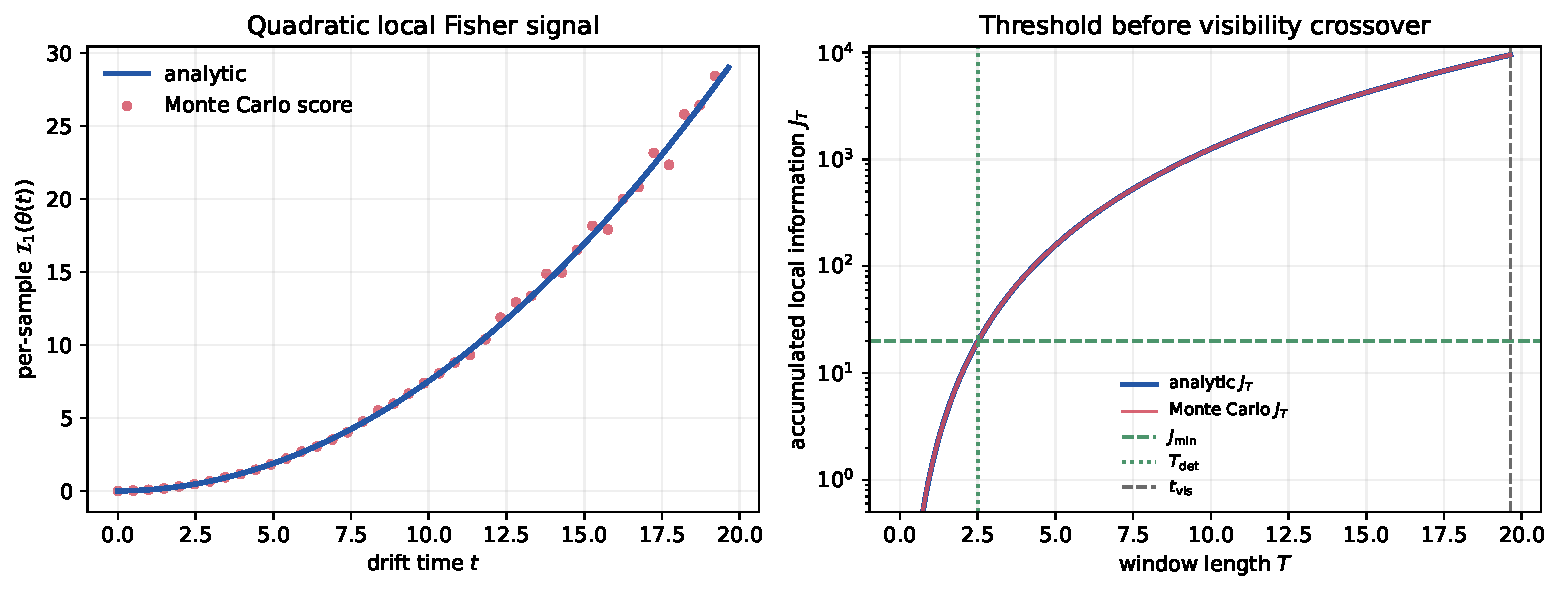
\includegraphics[width=\textwidth]{fig_fisher_residual.pdf}
\caption{\textbf{Direct score-based Fisher test.}
\textbf{Left:} analytic per-sample Fisher information and Monte Carlo
score-squared estimate, both quadratic in drift time.
\textbf{Right:} analytic and empirical accumulated local information;
the $J_{\min}=20$ crossing precedes the independently defined visibility
crossover for this parameter set.}
\label{T-III-fig:fisher_residual}
\end{figure}

% ------------------------------------------------------------
\subsection{Heuristic Calibration-Control Model}
\label{T-III-subsec:demo_model}

\paragraph{Environment.}
A $d$-dimensional linear prediction task:
$y(t) = \mathbf{w}(t)^\top \mathbf{x}(t)
+ \sigma\,\epsilon(t)$,
$\mathbf{x}(t) \sim \mathcal{N}(\mathbf{0}, \mathbf{I}_d)$,
$\epsilon \sim \mathcal{N}(0,1)$.
The weight vector $\mathbf{w}(t) \in \mathbb{S}^{d-1}$
drifts by receiving random perturbations on
\emph{background} dimensions only (indices $k,\ldots,d{-}1$),
then renormalising.  Signal therefore migrates progressively
from the ego's foreground to its blind sector.

\paragraph{Agents.}
\begin{itemize}
\item \textbf{Fixed ego} (Paper~II analogue):
  learns a linear model on a \emph{fixed} foreground
  subspace of dimension~$k$ via stochastic gradient descent
  (SGD, rate~$\eta$, decay~$\lambda$).
  Embodies the ``frozen gauge'' of Paper~II.
\item \textbf{Calibrated loop} (Paper~III analogue):
  identical ego plus a staleness sentinel and recalibration
  mechanism.
  The sentinel tracks $g_i = \mathrm{EMA}(|e\,x_i|)$ for
  each dimension~$i$ (an absolute-gradient proxy),
  computes the fraction of top-$k$ gradient dimensions
  \emph{not} in the current foreground as a frame-staleness
  index $m \in [0,1]$, and triggers
  recalibration when
  $\mathrm{EMA}(m) > \theta$.
  After recalibration, a settling period
  of~$\tau$ steps elapses before the sentinel resumes
  monitoring.
\end{itemize}

\paragraph{Parameters.}
\begin{center}
\small
\begin{tabular}{@{}lcl@{}}
\toprule
\textbf{Quantity} & \textbf{Value} & \textbf{Role} \\
\midrule
$d$ & 20 & full ambient dimension \\
$k$ & 5  & ego foreground dimension ($k/d = 0.25$) \\
$\sigma$ & 0.1 & observation noise std \\
$\eta$ & 0.01 & SGD learning rate \\
$\lambda$ & 0.998 & SGD weight decay \\
$\theta$ & 0.25 & staleness threshold \\
$\Lambda_{\mathrm{demo}}$ & variable & simulator drift amplitude per step \\
$\tau$ & variable & settling period (cooldown) \\
\bottomrule
\end{tabular}
\end{center}

\paragraph{Oracle metrics.}
Neither agent has access to $\mathbf{w}(t)$.
We evaluate performance externally using the \emph{oracle
full-space error}:
\begin{equation}
\label{T-III-eq:oracle_error}
\mathcal{E}_{\mathrm{full}}
= \bigl\|\mathbf{w}_{\mathrm{ego}}
  - \mathbf{w}^*_{\mathrm{fg}}\bigr\|^2
+ \bigl\|\mathbf{w}^*_{\mathrm{bg}}\bigr\|^2,
\end{equation}
where $\mathbf{w}^*_{\mathrm{fg}}$ and
$\mathbf{w}^*_{\mathrm{bg}}$ denote the true weight vector
restricted to foreground and background coordinates
respectively, and $\mathbf{w}_{\mathrm{ego}}$ is the ego's
foreground-supported estimator lifted to the full space.
The first term captures foreground tracking error (accessible
to the ego); the second captures hidden-sector signal
(invisible).

% ------------------------------------------------------------
\subsection{Results}
\label{T-III-subsec:demo_results}

\paragraph{Result 1: Delusion-correction separation
(Figure~\ref{T-III-fig:demo_trap}).}
At simulator drift amplitude $\Lambda_{\mathrm{demo}} = 0.02$,
settling period $\tau = 200$,
and $T = 5\,000$ steps, three phenomena are visible:

\begin{enumerate}
\item[(a)]
\emph{Delusion trap.}
The ego's foreground tracking error converges
to near zero, while the true full-space error rises
toward $\sim\!1$ and stabilises.
The growing gap between the two is the hidden sector in this supplied
linear model.  It does not prove a no-go theorem for all first-order
controllers.

\item[(b)]
\emph{Detectability.}
The staleness sentinel produces a clean sawtooth:
rising from zero after each recalibration, crossing the
threshold $\theta = 0.25$, and triggering frame reset
(25~events over $T = 5\,000$).
This demonstrates that the chosen overlap proxy can trigger a useful
reset.  The sentinel is not Fisher information; the direct Fisher test
is reported in Section~\ref{T-III-subsec:fisher_demo}.

\item[(c)]
\emph{Net benefit.}
The calibrated loop achieves
$\mathcal{E}_{\mathrm{full}} \approx 0.74$
versus the fixed ego's $\approx 1.02$:
a $27\%$ reduction in true prediction error.
\end{enumerate}

\begin{figure}[t]
\centering
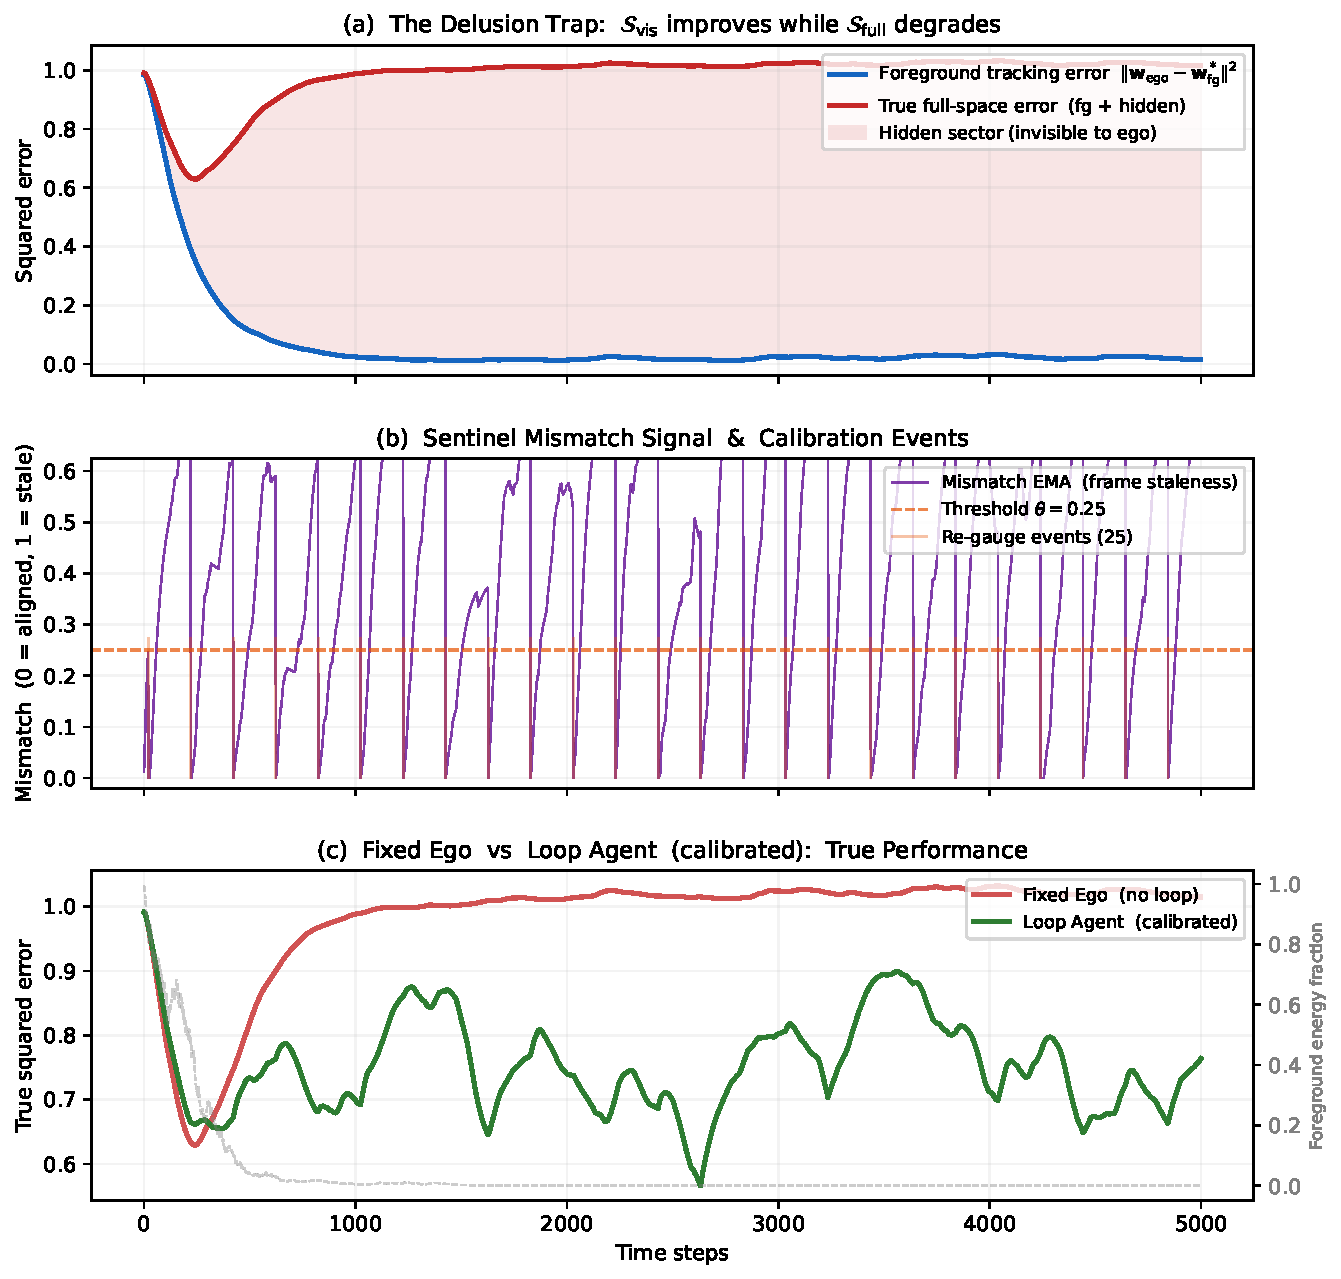
\includegraphics[width=\textwidth]{fig_delusion_trap.pdf}
\caption{%
\textbf{Delusion trap and calibration loop.}
$d = 20$, $k = 5$, $\Lambda_{\mathrm{demo}} = 0.02$,
$\tau = 200$,
$T = 5\,000$.
\textbf{(a)}~Foreground tracking error (blue) decreases
toward zero while true full-space error (red) increases;
the shaded region is the hidden sector, invisible to the ego.
\textbf{(b)}~Frame-staleness sentinel (purple) rises
monotonically between recalibration events (orange),
producing a sawtooth with 25 threshold crossings.
\textbf{(c)}~The calibrated loop (green) maintains
lower true error than the fixed ego (red);
the grey dashed line shows the foreground energy fraction
decaying as signal migrates to the background.}
\label{T-III-fig:demo_trap}
\end{figure}

\paragraph{Result 2: Phase structure and optimal
calibration budget
(Figures~\ref{T-III-fig:demo_phase}--\ref{T-III-fig:demo_alpha}).}
We scan 16 simulator drift amplitudes
$\Lambda_{\mathrm{demo}} \in [0.005, 0.08]$ and
16 settling periods $\tau \in [15, 800]$
(logarithmically spaced), running both agents for
$T = 4\,000$ steps across 6 random seeds per grid point.

Figure~\ref{T-III-fig:demo_phase}(a) shows the performance
gain $\Delta = \mathcal{E}_{\mathrm{ego}}
- \mathcal{E}_{\mathrm{loop}}$:
the loop improves over the ego (green) across most of
the parameter space, with a boundary at $\Delta = 0$
(dashed) below which recalibration is counterproductive
(very low drift, where the overhead of re-learning
exceeds the benefit of tracking).
The solid curve traces the \emph{optimal settling period}
$\tau_{\mathrm{opt}}(\Lambda_{\mathrm{demo}})$---the recalibration
period minimising $\mathcal{E}_{\mathrm{loop}}$---which
decreases monotonically from $\sim\!370$ steps at
$\Lambda_{\mathrm{demo}} = 0.005$ to $\sim\!100$ at
$\Lambda_{\mathrm{demo}} = 0.08$.
Figure~\ref{T-III-fig:demo_phase}(b) shows that calibration
frequency increases smoothly with drift and with shorter
settling period, exhibiting the cost--performance
trade-off of this supplied controller and cost proxy.  It does not test
Proposition~\ref{T-III-prop:loop_cost_impl}.

Extracting $\tau_{\mathrm{opt}}(\Lambda_{\mathrm{demo}})$ yields the
\emph{optimal calibration frequency}
$\alpha_{\mathrm{opt}}(\Lambda_{\mathrm{demo}})
= 1/\tau_{\mathrm{opt}}$
(Figure~\ref{T-III-fig:demo_alpha}).
The curve is smooth and monotonically increasing:
faster drift demands tighter calibration.
It saturates at high $\Lambda_{\mathrm{demo}}$ near
$\alpha_{\mathrm{opt}} \approx 0.01$ per step
($\tau_{\mathrm{opt}} \approx 100$), of the same
order as the learner's settling time.
This is consistent with the intuition that drift
estimation requires a minimum observation window;
the self-referential Cram\'{e}r--Rao bound
(Theorem~\ref{T-III-thm:SRCR}) provides the analytic
counterpart of this computational floor.

\begin{figure}[t]
\centering
\includegraphics[width=\textwidth]%
  {fig_phase_with_boundary.pdf}
\caption{%
\textbf{Phase structure and calibration cost.}
$16 \times 16$ grid, $T = 4\,000$, 6 seeds per point.
\textbf{(a)}~Performance gain $\Delta$; green = loop
improves on ego, red = counterproductive.
Solid curve: $\tau_{\mathrm{opt}}(\Lambda_{\mathrm{demo}})$.
Dashed: $\Delta = 0$ boundary.
\textbf{(b)}~Calibration frequency (thermodynamic cost
proxy: recalibration events per step, proportional to
energy expenditure under a fixed per-recalibration cost
model); $\tau_{\mathrm{opt}}$ overlaid.}
\label{T-III-fig:demo_phase}
\end{figure}

\begin{figure}[t]
\centering
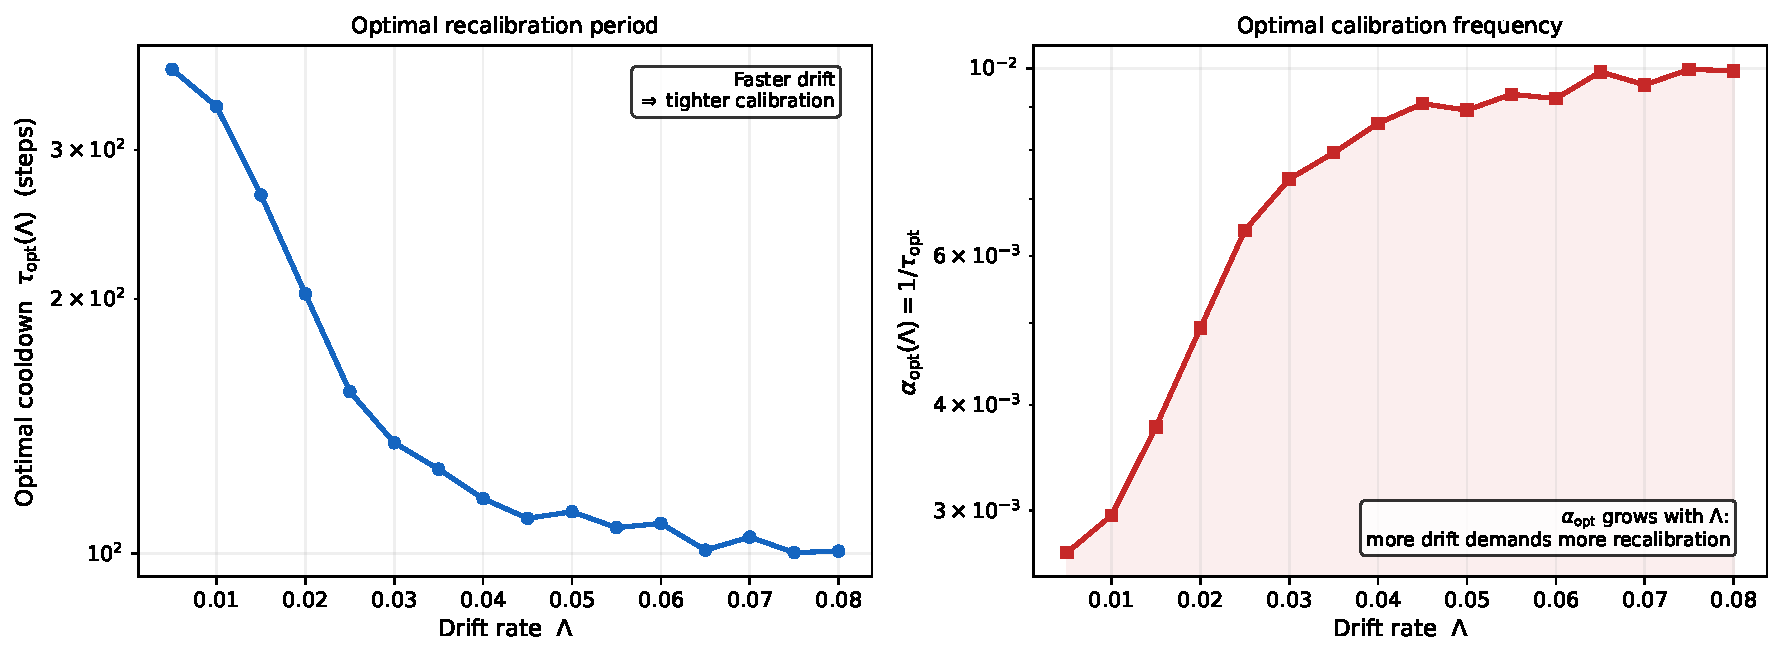
\includegraphics[width=\textwidth]{fig_alpha_opt.pdf}
\caption{%
\textbf{Optimal calibration frequency.}
\textbf{Left:}
$\tau_{\mathrm{opt}}(\Lambda_{\mathrm{demo}})$ decreases monotonically
with drift rate.
\textbf{Right:}
$\alpha_{\mathrm{opt}}(\Lambda_{\mathrm{demo}})
= 1/\tau_{\mathrm{opt}}$
increases with drift rate and saturates at the learner's
settling timescale ($\sim\!100$ steps), consistent with
an observation-window floor.}
\label{T-III-fig:demo_alpha}
\end{figure}

% ------------------------------------------------------------
\subsection{Scope of This Demonstration}
\label{T-III-subsec:demo_scope}

This demonstration \textbf{does} show:
\begin{enumerate}
\item The explicit Gaussian residual model has a directly measured
  score-squared Fisher signal with the quadratic and cubic scalings in
  Proposition~\ref{T-III-prop:gaussian_fisher}.
\item For the declared Gaussian parameters, the Fisher threshold is
  crossed before the linear visibility crossover.
\item A separate, non-Fisher frame-staleness proxy has clean threshold
  dynamics and triggers effective recalibration in the supplied linear
  controller.
\item An optimal calibration frequency
  $\alpha_{\mathrm{opt}}(\Lambda_{\mathrm{demo}})$ exists, increases
  monotonically with drift rate, and saturates at the
  learner's settling timescale in the scanned grid.
\end{enumerate}

\noindent
In summary, the direct experiment validates the declared Fisher
likelihood, while the controller experiment establishes a model-specific
proxy trade-off.  Neither is universal across architectures or
environment classes.

\medskip
This demonstration does \textbf{not} show:
\begin{enumerate}
\item That the specific functional form of
  $\alpha_{\mathrm{opt}}(\Lambda)$ matches the analytic
  Cram\'{e}r--Rao prediction in the
  large-$d$ limit.  The demonstration confirms the
  monotonic trend and saturation; deriving the exact
  scaling exponent from Theorem~\ref{T-III-thm:SRCR}
  remains open.
\item That the results generalise to all environment
  classes.  The model uses Gaussian features, linear
  regression, and isotropic background drift; extensions
  to non-linear, non-Gaussian, or structured-drift
  settings require further investigation.
\item That the calibration loop is optimal among all
  possible adaptive strategies.  It implements one
  specific realisation of the calibration-loop
  architecture.
\item That the gradient-overlap sentinel estimates Fisher information,
  or that recalibration-event frequency is a thermodynamic dissipation
  measurement.
\end{enumerate}

\paragraph{Reproducibility.}
\begin{sloppypar}
The controller simulation is in \texttt{tdome\_demo.py}.  The direct
Fisher experiment is in \texttt{fisher\_residual\_demo.py}, with raw
output in \texttt{fisher\_residual\_data.csv}.  Both require only NumPy
and Matplotlib and use fixed random seeds.
\end{sloppypar}

% ============================================================
\section{Discussion}
\label{T-III-sec:discussion}

% ------------------------------------------------------------
\subsection{Summary of Results}
\label{T-III-subsec:summary}

\begin{center}
\small
\setlength{\tabcolsep}{4pt}%
\begin{tabular}{@{}lP{6cm}c@{}}
\toprule
\textbf{Result} & \textbf{Statement} & \textbf{Sec.} \\
\midrule
Even-likelihood non-identifiability
  & The Gaussian residual record cannot identify mismatch sign
  & \ref{T-III-subsec:first_order} \\[3pt]
Drift Detectability
  & Per-sample FI is quadratic and accumulated local FI is cubic in the
    Gaussian linear-drift model
  & \ref{T-III-subsec:self_ref_fisher} \\[3pt]
Self-Referential CR Bound
  & Drift estimation bounded by
    $1/(n_{\mathrm{eff}}\,\mathbb E_\pi[\mathcal I_1]
    + \mathcal{I}_{\mathrm{ego}})$ under regular prior/likelihood data
  & \ref{T-III-subsec:SRCR} \\[3pt]
Loop Tracking Bound
  & Lyapunov $V$ with tracking neighbourhood
    $V_\infty = \|\dot{\sigma}^*\|^2/(\eta m_L)^2$ under local
    geodesic strong convexity
  & \ref{T-III-subsec:lyapunov} \\[3pt]
Four-Part Structure
  & Four supplied layers define the running model architecture
  & \ref{T-III-subsec:four_part} \\[3pt]
Loop Cost
  & $\dot{W}_{\mathrm{loop}} \geq k_BT\,\ln 2\,(R_s+R_c)
    + \mathcal{L}^2/\tau_{\mathrm{recalib}}^2$
    for a separable reset-based implementation
  & \ref{T-III-subsec:cost_theorem} \\[3pt]
Persistence Budget
  & Universal inherited budget withdrawn
  & \ref{T-III-subsec:persistence} \\[3pt]
Numerical Demonstration
  & Direct Fisher test plus a separate heuristic-controller scan
  & \ref{T-III-sec:numerical} \\
\bottomrule
\end{tabular}
\end{center}

% ------------------------------------------------------------
\subsection{Conditional Interface Sequence}
\label{T-III-subsec:logic_chain}

Papers~I--III provide a conditional interface sequence:

\begin{center}
\small
\setlength{\tabcolsep}{3pt}%
\begin{tabular}{@{}lP{3.2cm}P{3.8cm}l@{}}
\toprule
\textbf{Paper} & \textbf{Crisis} & \textbf{Resolution}
  & \textbf{What is born} \\
\midrule
Paper~I
  & Restricted autonomous baseline
  & Correlation-aware accounting
  & \textbf{Conditional resource model} \\[3pt]
Paper~II
  & Raw archive exceeds a declared budget
  & Supplied coordinate projection
  & \textbf{Frame model} \\[3pt]
Paper~III
  & Linear visibility loss in a fixed frame
  & Likelihood-based detection; conditional tracking
  & \textbf{Calibration model} \\
\bottomrule
\end{tabular}
\end{center}

The arrows are motivation or model interfaces.  The tracking theorem is
local and conditional, the universal persistence budget is withdrawn,
and no termination or completeness result follows.

% ------------------------------------------------------------
\subsection{What This Paper Does and Does Not Show}
\label{T-III-subsec:claims}

This paper \textbf{does} show:
\begin{enumerate}
\item The even Gaussian residual likelihood cannot identify mismatch
  sign, while its score has the explicit Fisher scalings in
  Proposition~\ref{T-III-prop:gaussian_fisher}.
\item Detection precedes visibility loss exactly when the threshold
  condition in Corollary~\ref{T-III-cor:detection_window} holds.
\item Drift estimation precision is bounded by the
  Self-Referential Cram\'{e}r--Rao bound
  (Theorem~\ref{T-III-thm:SRCR}).
\item The calibration loop tracks the optimal frame
  within a bounded neighbourhood under a Lyapunov
  tracking bound
  (Theorem~\ref{T-III-thm:loop_stability}).
\item A separable reset-based hardware model obeys the conditional cost
  bound in Proposition~\ref{T-III-prop:loop_cost_impl}.
\end{enumerate}

\medskip
This paper does \textbf{not} show:
\begin{enumerate}
\item That self-referential calibration implies or requires
  phenomenal consciousness, subjective experience, or
  qualia. ``Reflexivity'' as used here denotes
  second-order control, nothing more.
\item That the Lyapunov function $V$ is a measure of
  ``awareness.'' It is a control-theoretic stability
  condition, not a consciousness metric.
\item That the four-part template is necessary, sufficient, or a
  complete characterisation of agency.
\item That Fisher information requires the agent to
  ``know'' it is computing Fisher information.
  The computation can be implemented implicitly by any
  physical system whose dynamics approximate the natural
  gradient.
\item That the calibration loop eliminates the ego's bias.
  It tracks and compensates for drift in the bias;
  the four bias terms of Paper~II persist.
\item That sensing or computing is intrinsically dissipative.  The
  Landauer terms require irreversible register reset.
\item That this framework applies to all possible systems.
  It applies to systems satisfying~(C1)--(C5).
\item That the structural parallel with philosophical
  concepts of self-awareness constitutes a philosophical
  or metaphysical claim.
\item That the Clifford algebra is the only possible
  algebraic setting. Other control algebras may yield
  analogous results with different quantitative bounds.
\end{enumerate}

\medskip
We have established a checkable Gaussian Fisher signal, a regular
Bayesian estimation bound, and a local tracking result.  Their use in a
physical agent remains conditional on the declared observation,
optimization, and hardware models.

% ============================================================
% REFERENCES
% ============================================================


\backmatter

% ============================================================================
% UNIFIED BIBLIOGRAPHY
% ============================================================================
\begin{thebibliography}{99}

\bibitem{ABS1964}
M.~F.~Atiyah, R.~Bott and A.~Shapiro,
\emph{Clifford modules},
Topology \textbf{3}, Suppl.~1, 3--38 (1964).

\bibitem{Albert2000}
D. Z. Albert, \emph{Time and Chance}, Harvard University Press (2000).

\bibitem{AlfsenShultz2003}
E.~M.~Alfsen and F.~W.~Shultz, \emph{Geometry of State Spaces of Operator Algebras}, Birkh\"auser (2003).

\bibitem{Amari1985}
S.-i.~Amari,
\emph{Differential-Geometrical Methods in Statistics},
Lecture Notes in Statistics \textbf{28}, Springer (1985).

\bibitem{Amari1998}
S.-i.~Amari,
\emph{Natural gradient works efficiently in learning},
Neural Computation \textbf{10}, 251 (1998).

\bibitem{AmariNagaoka2000}
S.-i.~Amari and H.~Nagaoka,
\emph{Methods of Information Geometry},
Translations of Mathematical Monographs \textbf{191},
AMS (2000).

\bibitem{Araki1999}
H. Araki, \emph{Mathematical Theory of Quantum Fields}, Oxford University Press (1999).

\bibitem{Asanga_Mahayana}
Asaṅga, \emph{Mahāyānasaṃgraha (Summary of the Great Vehicle)}, trans.\ É. Lamotte, Peeters (1973).

\bibitem{Ashby1956}
W.~R.~Ashby,
\emph{An Introduction to Cybernetics},
Chapman \& Hall (1956).

\bibitem{AstromWittenmark1995}
K.~J.~\AA{}str\"{o}m and B.~Wittenmark,
\emph{Adaptive Control},
2nd ed., Addison-Wesley (1995).

\bibitem{BaratoSeifert2015}
A.~C.~Barato and U.~Seifert,
\emph{Thermodynamic uncertainty relation for biomolecular
processes},
Phys.\ Rev.\ Lett.\ \textbf{114}, 158101 (2015).

\bibitem{Barrett2007}
J.~W.~Barrett, \emph{A Lorentzian version of the non-commutative geometry of the standard model of particle physics}, J. Math. Phys. \textbf{48}, 012303 (2007).

\bibitem{Bengtsson2006}
I. Bengtsson and K. \.Zyczkowski, \emph{Geometry of Quantum States: An Introduction to Quantum Entanglement}, Cambridge University Press (2006).

\bibitem{Bennett1982}
C.~H.~Bennett,
\emph{The thermodynamics of computation---a review},
Int.\ J.\ Theor.\ Phys.\ \textbf{21}, 905 (1982).

\bibitem{BialekNemenmanTishby2001}
W.~Bialek, I.~Nemenman, and N.~Tishby,
\emph{Predictability, complexity, and learning},
Neural Computation \textbf{13}, 2409 (2001).

\bibitem{BisognanoWichmann1975}
J.~J.~Bisognano and E.~H.~Wichmann,
\emph{On the duality condition for a Hermitian scalar field},
J.\ Math.\ Phys.\ \textbf{16}, 985 (1975).

\bibitem{BisognanoWichmann1976}
J.~J.~Bisognano and E.~H.~Wichmann,
\emph{On the duality condition for quantum fields},
J.\ Math.\ Phys.\ \textbf{17}, 303 (1976).

\bibitem{Boltzmann1896}
L. Boltzmann, \emph{Vorlesungen \"uber Gastheorie}, J. A. Barth, Leipzig (1896).

\bibitem{BratteliRobinson1997}
O.~Bratteli and D.~W.~Robinson,
\emph{Operator Algebras and Quantum Statistical Mechanics},
Vols.\ 1--2, 2nd ed., Springer (1997).

\bibitem{Breuer2002}
H.-P.~Breuer and F.~Petruccione, \emph{The Theory of Open Quantum Systems}, Oxford University Press (2002).

\bibitem{BreuerLainePiilo2009}
H.-P.~Breuer, E.-M.~Laine, and J.~Piilo,
\emph{Measure for the Degree of Non-Markovian Behavior of Quantum Processes in Open Systems},
Phys.\ Rev.\ Lett.\ \textbf{103}, 210401 (2009).

\bibitem{BreuerPetruccione2002}
H.-P.~Breuer and F.~Petruccione,
\emph{The Theory of Open Quantum Systems},
Oxford University Press (2002).

\bibitem{Carroll2010}
S. Carroll, \emph{From Eternity to Here: The Quest for the Ultimate Theory of Time}, Dutton (2010).

\bibitem{CarrollSingh2021}
S.~M.~Carroll and A.~Singh,
\emph{Quantum mereology: Factorizing Hilbert space into subsystems with quasiclassical dynamics},
Phys.\ Rev.\ A \textbf{103}, 022213 (2021).

\bibitem{CasiniHuertaMyers2011}
H.~Casini, M.~Huerta, and R.~C.~Myers,
\emph{Towards a derivation of holographic entanglement entropy},
JHEP \textbf{1105}, 036 (2011),
arXiv:1102.0440.

\bibitem{Cencov1982}
N.~N.~\v{C}encov,
\emph{Statistical Decision Rules and Optimal Inference},
Translations of Mathematical Monographs \textbf{53},
AMS (1982).

\bibitem{Chalmers1996}
D. J. Chalmers, \emph{The Conscious Mind: In Search of a Fundamental Theory}, Oxford University Press (1996).

% Neuroscience

\bibitem{Connes1994}
A.~Connes, \emph{Noncommutative Geometry}, Academic Press (1994).

\bibitem{Cotler2019}
J.~Cotler, G.~Penington, and D.~H.~Ranard,
\emph{Locality from the spectrum},
Commun.\ Math.\ Phys.\ \textbf{368}, 1267--1296 (2019).

\bibitem{CoverThomas2006}
T.~M.~Cover and J.~A.~Thomas,
\emph{Elements of Information Theory},
2nd ed., Wiley (2006).

\bibitem{Crooks2007}
G.~E.~Crooks,
\emph{Measuring thermodynamic length},
Phys.\ Rev.\ Lett.\ \textbf{99}, 100602 (2007).

\bibitem{CrutchfieldYoung1989}
J.~P.~Crutchfield and K.~Young,
\emph{Inferring statistical complexity},
Phys.\ Rev.\ Lett.\ \textbf{63}, 105 (1989).

\bibitem{DeWitt1967}
B. S. DeWitt, \emph{Quantum Theory of Gravity. I. The Canonical Theory}, Phys. Rev. \textbf{160}, 1113 (1967).

\bibitem{Diehl2008}
S.~Diehl, A.~Micheli, A.~Kantian, B.~Kraus, H.~P.~B\"uchler, and P.~Zoller, \emph{Quantum states and phases in driven open quantum systems with cold atoms}, Nat. Phys. \textbf{4}, 878--883 (2008).

\bibitem{DoplicherLongo1984}
S.~Doplicher and R.~Longo, \emph{Standard and split inclusions of von Neumann algebras}, Invent. Math. \textbf{75}, 493--536 (1984).

\bibitem{Doran2003}
C.~Doran and A.~Lasenby, \emph{Geometric Algebra for Physicists}, Cambridge University Press (2003).

\bibitem{Eisert2010}
J.~Eisert, M.~Cramer, and M.~B.~Plenio,
\emph{Colloquium: Area laws for the entanglement entropy},
Rev.\ Mod.\ Phys.\ \textbf{82}, 277 (2010).

\bibitem{EspositoLindenbergVandenBroeck2010}
M.~Esposito, K.~Lindenberg, and C.~Van~den~Broeck,
\emph{Entropy production as correlation between system and reservoir},
New J.\ Phys.\ \textbf{12}, 013013 (2010).

\bibitem{Faulkner2014}
T. Faulkner, M. Guica, T. Hartman, R. C. Myers, and M. Van Raamsdonk, \emph{Gravitation from Entanglement in Holographic CFTs}, JHEP \textbf{03}, 051 (2014).

\bibitem{Fitzsimons2015}
J.~F.~Fitzsimons, J.~A.~Jones, and V.~Vedral,
\emph{Quantum correlations which imply causation},
Sci.\ Rep.\ \textbf{5}, 18281 (2015).

\bibitem{French2014}
S. French, \emph{The Structure of the World: Metaphysics and Representation}, Oxford University Press (2014).

% Buddhist Primary Texts (Yogacara)

\bibitem{Fuchs2014}
C. A. Fuchs, \emph{QBism, the Perimeter of Quantum Bayesianism}, arXiv:1003.5209 (2014).

\bibitem{FuchsMerminSchack2014}
C. A. Fuchs, N. D. Mermin, and R. Schack, \emph{An Introduction to QBism with an Application to the Locality of Quantum Mechanics}, Am. J. Phys. \textbf{82}, 749 (2014).

\bibitem{GKS1976}
V.~Gorini, A.~Kossakowski, and E.~C.~G.~Sudarshan,
\emph{Completely positive dynamical semigroups of $N$-level systems},
J.\ Math.\ Phys.\ \textbf{17}, 821 (1976).

\bibitem{Garfield2002}
J. L. Garfield, \emph{Empty Words: Buddhist Philosophy and Cross-Cultural Interpretation}, Oxford University Press (2002).

\bibitem{Gombrich1996}
R. F. Gombrich, \emph{How Buddhism Began: The Conditioned Genesis of the Early Teachings}, Athlone Press (1996).

\bibitem{GovernTenWolde2014}
W.~P.~Govern and P.~R.~ten~Wolde,
\emph{Optimal resource allocation in cellular sensing systems},
Proc.\ Natl.\ Acad.\ Sci.\ USA \textbf{111}, 17486 (2014).

\bibitem{Graybiel2008}
A. M. Graybiel, \emph{Habits, rituals, and the evaluative brain}, Annual Review of Neuroscience \textbf{31}, 359--387 (2008).

\bibitem{Gunaydin1973}
M.~G\"unaydin and F.~G\"ursey, \emph{Quark structure and octonions}, J.\ Math.\ Phys.\ \textbf{14}, 1651 (1973).

\bibitem{Haag1996}
R. Haag, \emph{Local Quantum Physics: Fields, Particles, Algebras}, Springer-Verlag (1996).

\bibitem{Haagerup1975}
U.~Haagerup,
\emph{The standard form of von Neumann algebras},
Math.\ Scand.\ \textbf{37}, 271--283 (1975).

\bibitem{Haggard2005}
P. Haggard, \emph{Conscious intention and motor cognition}, Trends in Cognitive Sciences \textbf{9}(6), 290--295 (2005).

\bibitem{Harvey2000}
P. Harvey, \emph{An Introduction to Buddhist Ethics: Foundations, Values and Issues}, Cambridge University Press (2000).

% Early Buddhist Texts

\bibitem{Hastings2007}
M.~B.~Hastings,
\emph{An area law for one-dimensional quantum systems},
J.\ Stat.\ Mech.\ \textbf{2007}, P08024 (2007),
arXiv:0705.2024.

\bibitem{Hayden2007}
P. Hayden and J. Preskill, \emph{Black holes as mirrors: quantum information in random subsystems}, JHEP \textbf{09}, 120 (2007).

\bibitem{HaydenLeungWinter2006}
P.~Hayden, D.~W.~Leung, and A.~Winter,
\emph{Aspects of generic entanglement},
Commun.\ Math.\ Phys.\ \textbf{265}, 95--117 (2006).

\bibitem{HaydenPreskill2007}
P. Hayden and J. Preskill, \emph{Black holes as mirrors: quantum information in random subsystems}, JHEP \textbf{09}, 120 (2007).

\bibitem{Hestenes1966}
D.~Hestenes, \emph{Space-Time Algebra}, Gordon and Breach (1966).

\bibitem{Ito2018}
S.~Ito,
\emph{Stochastic thermodynamic interpretation of
information geometry},
Phys.\ Rev.\ Lett.\ \textbf{121}, 030605 (2018).

\bibitem{JLMS2016}
D.~L.~Jafferis, A.~Lewkowycz, J.~Maldacena, and S.~J.~Suh,
\emph{Relative entropy equals bulk relative entropy},
JHEP \textbf{1606}, 004 (2016),
arXiv:1512.06431.

\bibitem{Jacobson1995}
T. Jacobson, \emph{Thermodynamics of Spacetime: The Einstein Equation of State}, Phys. Rev. Lett. \textbf{75}, 1260 (1995).

\bibitem{Jacobson2016}
T.~Jacobson,
\emph{Entanglement equilibrium and the Einstein equation},
Phys.\ Rev.\ Lett.\ \textbf{116}, 201101 (2016),
arXiv:1505.04753.

\bibitem{Jarzynski2011}
C.~Jarzynski, \emph{Equalities and inequalities: irreversibility and the second law at the nanoscale}, Annu.\ Rev.\ Condens.\ Matter Phys.\ \textbf{2}, 329 (2011).

\bibitem{JohnsonLindenstrauss1984}
W.~B.~Johnson and J.~Lindenstrauss,
\emph{Extensions of Lipschitz mappings into a Hilbert space},
Contemp.\ Math.\ \textbf{26}, 189 (1984).

\bibitem{Kiefer2012}
C. Kiefer, \emph{Quantum Gravity}, 3rd ed., Oxford University Press (2012).

\bibitem{Kleene1952}
S. C. Kleene, \emph{Introduction to Metamathematics}, North-Holland (1952).

\bibitem{Ladyman2007}
J. Ladyman and D. Ross, \emph{Every Thing Must Go: Metaphysics Naturalized}, Oxford University Press (2007).

\bibitem{Landauer1961}
R.~Landauer,
\emph{Irreversibility and heat generation in the computing process},
IBM J.\ Res.\ Dev.\ \textbf{5}, 183 (1961).

\bibitem{Lashkari2014}
N. Lashkari, M. B. McDermott, and M. Van Raamsdonk, \emph{Gravitational dynamics from entanglement ``thermodynamics''}, JHEP \textbf{04}, 195 (2014).

\bibitem{LaudisaRovelli2021}
F. Laudisa and C. Rovelli, \emph{Relational Quantum Mechanics}, Stanford Encyclopedia of Philosophy (2021).

\bibitem{LawsonMichelsohn1989}
H.~B.~Lawson and M.-L.~Michelsohn,
\emph{Spin Geometry},
Princeton University Press (1989).

\bibitem{Lawvere1969}
F. W. Lawvere, \emph{Diagonal arguments and cartesian closed categories}, in \emph{Category Theory, Homology Theory and their Applications II}, Lecture Notes in Mathematics \textbf{92}, 134--145 (1969).

\bibitem{LeiferSpekkens2013}
M.~S.~Leifer and R.~W.~Spekkens,
\emph{Towards a formulation of quantum theory as a causally neutral theory of Bayesian inference},
Phys.\ Rev.\ A \textbf{88}, 052130 (2013).

\bibitem{Levine1983}
J. Levine, \emph{Materialism and qualia: The explanatory gap}, Pacific Philosophical Quarterly \textbf{64}, 354 (1983).

\bibitem{Lidar2003}
D.~A.~Lidar and K.~B.~Whaley, \emph{Decoherence-free subspaces and subsystems}, in \emph{Irreversible Quantum Dynamics}, Springer, pp.\ 83--120 (2003).

\bibitem{Lindblad1976}
G.~Lindblad,
\emph{On the generators of quantum dynamical semigroups},
Commun.\ Math.\ Phys.\ \textbf{48}, 119 (1976).

\bibitem{Lusthaus2002}
D. Lusthaus, \emph{Buddhist Phenomenology: A Philosophical Investigation of Yogācāra Buddhism and the Ch'eng Wei-shih lun}, Routledge (2002).

\bibitem{Maldacena1999}
J. M. Maldacena, \emph{The Large N limit of superconformal field theories and supergravity}, Int. J. Theor. Phys. \textbf{38}, 1113 (1999).

\bibitem{MehtaSchwab2012}
P.~Mehta and D.~J.~Schwab,
\emph{Energetic costs of cellular computation},
Proc.\ Natl.\ Acad.\ Sci.\ USA \textbf{109}, 17978 (2012).

\bibitem{Mirrahimi2005}
M.~Mirrahimi, P.~Rouchon, and G.~Turinici, \emph{Lyapunov control of bilinear Schr\"odinger equations}, Automatica \textbf{41}, 1987--1994 (2005).

\bibitem{Nagarjuna_MMK_Garfield1995}
Nāgārjuna, \emph{The Fundamental Wisdom of the Middle Way: Nāgārjuna's Mūlamadhyamakakārikā}, trans.\ J. L. Garfield, Oxford University Press (1995).

% Buddhist Secondary Sources

\bibitem{Nakajima1958}
S.~Nakajima,
\emph{On quantum theory of transport phenomena},
Prog.\ Theor.\ Phys.\ \textbf{20}, 948 (1958).

\bibitem{Page1993}
D. N. Page, \emph{Average entropy of a subsystem}, Phys. Rev. Lett. \textbf{71}, 1291 (1993).

\bibitem{PageWootters1983}
D. N. Page and W. K. Wootters, \emph{Evolution without evolution: Dynamics described by stationary observables}, Phys. Rev. D \textbf{27}, 2885 (1983).

\bibitem{Parrondo2015}
J.~M.~R.~Parrondo, J.~M.~Horowitz, and T.~Sagawa, \emph{Thermodynamics of information}, Nat.\ Phys.\ \textbf{11}, 131 (2015).

\bibitem{PaschkeSitarz2006}
M.~Paschke and A.~Sitarz, \emph{Equivariant Lorentzian spectral triples}, arXiv:math-ph/0611029 (2006).

\bibitem{Pearl2009}
J. Pearl, \emph{Causality: Models, Reasoning, and Inference}, 2nd ed., Cambridge University Press (2009).

\bibitem{Penrose1989}
R. Penrose, \emph{The Emperor's New Mind}, Oxford University Press (1989).

\bibitem{Penrose2010}
R. Penrose, \emph{Cycles of Time: An Extraordinary New View of the Universe}, Bodley Head (2010).

\bibitem{Petz1996}
D. Petz, \emph{Monotone metrics on matrix spaces}, Linear Algebra Appl. \textbf{244}, 81 (1996).

\bibitem{PooleOzairVanDenOord2019}
B.~Poole, S.~Ozair, A.~Van~Den~Oord, A.~Alemi, and G.~Tucker,
\emph{On variational bounds of mutual information},
Proc.\ ICML, PMLR \textbf{97}, 5171--5180 (2019).

\bibitem{Price2012}
H. Price, \emph{Does Time-Symmetry Imply Retrocausality?}, Found. Phys. \textbf{42}, 724 (2012).

\bibitem{Rao1945}
C.~R.~Rao,
\emph{Information and the accuracy attainable in the
estimation of statistical parameters},
Bull.\ Calcutta Math.\ Soc.\ \textbf{37}, 81 (1945).

\bibitem{RivasHuelgaPlenio2014}
\'{A}.~Rivas, S.~F.~Huelga, and M.~B.~Plenio,
\emph{Quantum non-Markovianity: characterization, quantification and detection},
Rep.\ Prog.\ Phys.\ \textbf{77}, 094001 (2014).

\bibitem{Rovelli1996}
C. Rovelli, \emph{Relational Quantum Mechanics}, Int. J. Theor. Phys. \textbf{35}, 1637 (1996).

\bibitem{Rovelli2004}
C. Rovelli, \emph{Quantum Gravity}, Cambridge University Press (2004).

\bibitem{RyuTakayanagi2006}
S. Ryu and T. Takayanagi, \emph{Holographic Derivation of Entanglement Entropy from AdS/CFT}, Phys. Rev. Lett. \textbf{96}, 181602 (2006).

\bibitem{Sagawa2012}
T.~Sagawa and M.~Ueda, \emph{Fluctuation theorem with information exchange}, Phys.\ Rev.\ E \textbf{85}, 021104 (2012).

\bibitem{SagawaUeda2010}
T.~Sagawa and M.~Ueda,
\emph{Generalized Jarzynski Equality under Nonequilibrium Feedback Control},
Phys.\ Rev.\ Lett.\ \textbf{104}, 090602 (2010).

\bibitem{SagawaUeda2012}
T.~Sagawa and M.~Ueda,
\emph{Fluctuation Theorem with Information Exchange},
Phys.\ Rev.\ Lett.\ \textbf{109}, 180602 (2012).

\bibitem{Schafer1966}
R.~D.~Schafer, \emph{An Introduction to Nonassociative Algebras}, Academic Press (1966).

\bibitem{Schrodinger1944}
E.~Schr\"odinger,
\emph{What is Life?},
Cambridge University Press (1944).

\bibitem{Scott1972}
D. Scott, \emph{Continuous lattices}, in \emph{Toposes, Algebraic Geometry and Logic}, Lecture Notes in Mathematics \textbf{274}, 97--136 (1972).

\bibitem{Seifert2012}
U.~Seifert, \emph{Stochastic thermodynamics, fluctuation theorems and molecular machines}, Rep.\ Prog.\ Phys.\ \textbf{75}, 126001 (2012).

\bibitem{ShaliziCrutchfield2001}
C.~R.~Shalizi and J.~P.~Crutchfield,
\emph{Computational mechanics: Pattern and prediction, structure and simplicity},
J.\ Stat.\ Phys.\ \textbf{104}, 817 (2001).

\bibitem{Shannon1959}
C.~E.~Shannon,
\emph{Coding theorems for a discrete source with a
fidelity criterion},
IRE Nat.\ Conv.\ Rec., Part~4, pp.~142--163 (1959).

\bibitem{Siderits2007}
M. Siderits, \emph{Buddhism as Philosophy: An Introduction}, Hackett Publishing (2007).

% Karma Studies

\bibitem{Simon1955}
H.~A.~Simon,
\emph{A behavioral model of rational choice},
Quarterly J.\ of Economics \textbf{69}, 99 (1955).

\bibitem{Sims2003}
C.~A.~Sims,
\emph{Implications of rational inattention},
J.\ Monetary Economics \textbf{50}, 665 (2003).

\bibitem{SivakCrooks2012}
D.~A.~Sivak and G.~E.~Crooks,
\emph{Thermodynamic metrics and optimal paths},
Phys.\ Rev.\ Lett.\ \textbf{108}, 190602 (2012).

\bibitem{Smolin2006}
L. Smolin, \emph{The case for background independence}, in \emph{The Structural Foundations of Quantum Gravity}, eds. D. Rickles, S. French, J. Saatsi, Oxford University Press (2006).

\bibitem{Spohn1978}
H.~Spohn,
\emph{Entropy production for quantum dynamical semigroups},
J.\ Math.\ Phys.\ \textbf{19}, 1227 (1978).

\bibitem{SuttaNipata}
\emph{Sutta Nipāta}, in \emph{The Group of Discourses (Sutta Nipāta)}, trans.\ K. R. Norman, Pali Text Society (2001).

\bibitem{Swingle2012}
B. Swingle, \emph{Entanglement Renormalization and Holography}, Phys. Rev. D \textbf{86}, 065007 (2012).

\bibitem{Takesaki2003}
M.~Takesaki,
\emph{Theory of Operator Algebras II},
Encyclopaedia of Mathematical Sciences \textbf{125}, Springer (2003).

\bibitem{Tarski1955}
A. Tarski, \emph{A lattice-theoretical fixpoint theorem and its applications}, Pacific J. Math. \textbf{5}, 285--309 (1955).

\bibitem{Tegmark2000}
M.~Tegmark,
\emph{Importance of quantum decoherence in brain processes},
Phys.\ Rev.\ E \textbf{61}, 4194--4206 (2000).

% Structural Realism

\bibitem{Thiemann2007}
T. Thiemann, \emph{Modern Canonical Quantum General Relativity}, Cambridge University Press (2007).

\bibitem{TicozziViola2008}
F.~Ticozzi and L.~Viola, \emph{Quantum Markovian subsystems: invariance, attractivity, and control}, IEEE Trans. Autom. Control \textbf{53}, 2048--2063 (2008).

\bibitem{Tishby2000}
N.~Tishby, F.~C.~Pereira, and W.~Bialek,
\emph{The information bottleneck method},
in Proc.\ 37th Allerton Conf.\ on Communication, Control,
and Computing (1999); arXiv:physics/0004057 (2000).

\bibitem{VanRaamsdonk2010}
M. Van Raamsdonk, \emph{Building up spacetime with quantum entanglement}, Gen. Relativ. Gravit. \textbf{42}, 2323 (2010).

\bibitem{VandenDungen2016}
K.~van den Dungen, \emph{Krein spectral triples and the fermionic action}, Math. Phys. Anal. Geom. \textbf{19}, 4 (2016).

\bibitem{Vasubandhu_Trimsika}
Vasubandhu, \emph{Triṃśikā-vijñaptimātratā (Thirty Verses on Consciousness Only)}, trans.\ S. Anacker, in \emph{Seven Works of Vasubandhu}, Motilal Banarsidass (1984).

% Buddhist Primary Texts (Madhyamaka)

\bibitem{Verlinde2011}
E.~Verlinde, \emph{On the Origin of Gravity and the Laws of Newton}, JHEP \textbf{04}, 029 (2011).

\bibitem{Verstraete2009}
F.~Verstraete, M.~M.~Wolf, and J.~I.~Cirac, \emph{Quantum computation and quantum-state engineering driven by dissipation}, Nat. Phys. \textbf{5}, 633--636 (2009).

\bibitem{Vidal2008}
G. Vidal, \emph{Class of quantum many-body states that can be efficiently simulated}, Phys. Rev. Lett. \textbf{101}, 110501 (2008).

\bibitem{Viola2004}
H. Barnum, E. Knill, G. Ortiz, R. Somma, and L. Viola, \emph{A Subsystem-Independent Generalization of Entanglement}, Phys. Rev. Lett. \textbf{92}, 107902 (2004).

\bibitem{Waldron2003}
W. S. Waldron, \emph{The Buddhist Unconscious: The Ālaya-vijñāna in the Context of Indian Buddhist Thought}, Routledge (2003).

\bibitem{Wallace2010}
D. Wallace, \emph{Gravity, entropy, and cosmology: in search of clarity}, Brit. J. Phil. Sci. \textbf{61}, 513--540 (2010).

\bibitem{Wallace2012}
D. Wallace, \emph{The Emergent Multiverse}, Oxford University Press (2012).

\bibitem{Wallace2012Time}
D. Wallace, \emph{The Emergent Multiverse: Quantum Theory according to the Everett Interpretation}, Oxford University Press (2012), Chapter 8.

\bibitem{Weiss2012}
U.~Weiss, \emph{Quantum Dissipative Systems}, 4th ed., World Scientific (2012).

\bibitem{Wiesbrock1993}
H.-W.~Wiesbrock,
\emph{Half-sided modular inclusions of von Neumann algebras},
Commun.\ Math.\ Phys.\ \textbf{157}, 83 (1993).

\bibitem{WisemanMilburn2009}
H.~M.~Wiseman and G.~J.~Milburn, \emph{Quantum Measurement and Control}, Cambridge University Press (2009).

\bibitem{Witten2018}
E.~Witten, \emph{APS Medal for Exceptional Achievement in Research: Invited article on entanglement properties of quantum field theory}, Rev.\ Mod.\ Phys.\ \textbf{90}, 045003 (2018).

\bibitem{Wolf2006}
M.~M.~Wolf,
\emph{Violation of the entropic area law for fermions},
Phys.\ Rev.\ Lett.\ \textbf{96}, 010404 (2006).

\bibitem{Woodward2003}
J. Woodward, \emph{Making Things Happen: A Theory of Causal Explanation}, Oxford University Press (2003).

\bibitem{Yin2006}
H. H. Yin and B. J. Knowlton, \emph{The role of the basal ganglia in habit formation}, Nature Reviews Neuroscience \textbf{7}, 464--476 (2006).

\bibitem{Yngvason2005}
J.~Yngvason,
\emph{The role of type III factors in quantum field theory},
Rep.\ Math.\ Phys.\ \textbf{55}, 135 (2005),
arXiv:math-ph/0411058.

\bibitem{Zanardi2001}
P. Zanardi, \emph{Virtual Quantum Subsystems}, Phys. Rev. Lett. \textbf{87}, 077901 (2001).

\bibitem{Zanardi2004}
P. Zanardi, D. A. Lidar, and S. Lloyd, \emph{Quantum Tensor Product Structures are Observable Induced}, Phys. Rev. Lett. \textbf{92}, 060402 (2004).

\bibitem{Zurek2003}
W. H. Zurek, \emph{Decoherence, einselection, and the quantum origins of the classical}, Rev. Mod. Phys. \textbf{75}, 715 (2003).

\bibitem{Zurek2009}
W. H. Zurek, \emph{Quantum Darwinism}, Nature Physics \textbf{5}, 181 (2009).

\bibitem{Zwanzig1960}
R.~Zwanzig,
\emph{Ensemble method in the theory of irreversibility},
J.\ Chem.\ Phys.\ \textbf{33}, 1338 (1960).

\bibitem{vanTrees1968}
H.~L.~van Trees,
\emph{Detection, Estimation, and Modulation Theory},
Part~I, Wiley (1968).

\bibitem{vonFoerster2003}
H.~von Foerster,
\emph{Understanding Understanding: Essays on Cybernetics
and Cognition},
Springer (2003).

\bibitem{Liu2026}
S.~Liu, \emph{Emergent Geometry from Coarse-Grained Observable Algebras: The Holographic Alaya-Field Framework}, Zenodo (2026), DOI: 10.5281/zenodo.18361706.

\bibitem{Liu2026HAFF_A}
S.~Liu, \emph{Emergent Geometry from Coarse-Grained Observable Algebras: The Holographic Alaya-Field Framework}, Zenodo (2026), DOI: 10.5281/zenodo.18361706.

\bibitem{Liu2026HAFF_B}
S.~Liu, \emph{Accessibility, Stability, and Emergent Geometry: Conceptual Clarifications on the Holographic Alaya-Field Framework}, Zenodo (2026), DOI: 10.5281/zenodo.18367060.

\bibitem{Liu2026HAFF_C}
S.~Liu, \emph{Causation, Agency, and Existence: Structural Constraints and Interpretive Bridges}, Zenodo (2026), DOI: 10.5281/zenodo.18374805.

\bibitem{Liu2026HAFF_F}
S.~Liu, \emph{Accessibility Propagation and Temporal Direction: A Conditional Structural Analysis}, Zenodo (2026), DOI: 10.5281/zenodo.18400425.

\bibitem{Liu2026HAFF_G}
S.~Liu, \emph{Structural Limits of Unification: Accessibility, Incompleteness, and a Programme-Level Final-Cut Diagnosis}, Zenodo (2026), DOI: 10.5281/zenodo.18402907.

\bibitem{Liu2026PaperA}
S.~Liu, \emph{Emergent Geometry from Coarse-Grained Observable Algebras: The Holographic Alaya-Field Framework}, Zenodo (2026), DOI: 10.5281/zenodo.18361706.

\bibitem{Liu2026PaperB}
S.~Liu, \emph{Accessibility, Stability, and Emergent Geometry: Conceptual Clarifications on the Holographic Alaya-Field Framework}, Zenodo (2026), DOI: 10.5281/zenodo.18367060.

\bibitem{Liu2026PaperC}
S.~Liu, \emph{Causation, Agency, and Existence: Structural Constraints and Interpretive Bridges}, Zenodo (2026), DOI: 10.5281/zenodo.18374805.

\bibitem{Liu2026PaperD}
S.~Liu, \emph{Observable-Algebra Selection and Emergent Gravitational Phenomena: A Conditional Structural Analysis}, Zenodo (2026), DOI: 10.5281/zenodo.18388881.

\bibitem{Liu2026PaperE}
S.~Liu, \emph{Measurement as Accessibility: A Structural Analysis of Observable Algebra Selection}, Zenodo (2026), DOI: 10.5281/zenodo.18400065.

\bibitem{Liu2026PaperF}
S.~Liu, \emph{Accessibility Propagation and Temporal Direction: A Conditional Structural Analysis}, Zenodo (2026), DOI: 10.5281/zenodo.18400425.

\bibitem{Liu2026PaperG}
S.~Liu, \emph{Structural Limits of Unification: Accessibility, Incompleteness, and a Programme-Level Final-Cut Diagnosis}, Zenodo (2026), DOI: 10.5281/zenodo.18402907.

\bibitem{Liu2026QRAIF_A}
S.~Liu, \emph{A Clifford-Encoding Model for Lorentzian Metrics in Entropic Gravity Frameworks}, Zenodo (2026), DOI: 10.5281/zenodo.18525876.

\bibitem{Liu2026QRAIF_B}
S.~Liu, \emph{Thermodynamic Stability Constraints on the Operator Algebra of Persistent Open Quantum Subsystems}, Zenodo (2026), DOI: 10.5281/zenodo.18525890.

\bibitem{Liu2026QRAIF_C}
S.~Liu, \emph{Conditional Image-Level Closure in the Q-RAIF Framework}, Zenodo (2026), DOI: 10.5281/zenodo.18528934.

\bibitem{Liu2026TDOME_I}
S.~Liu, \emph{Non-Markovian Memory and Temporal Accumulation: A Conditional Thermodynamic Analysis}, Zenodo (2026), DOI: 10.5281/zenodo.18574342.

\bibitem{Liu2026TDOME_II}
S.~Liu, \emph{Spontaneous Symmetry Breaking of Reference Frames as a Computational Cost Minimization Strategy}, Zenodo (2026), DOI: 10.5281/zenodo.18579703.

\end{thebibliography}

\end{document}
